% Options for packages loaded elsewhere
\PassOptionsToPackage{unicode}{hyperref}
\PassOptionsToPackage{hyphens}{url}
%
\documentclass[
  oneside]{book}
\usepackage{amsmath,amssymb}
\usepackage{lmodern}
\usepackage{ifxetex,ifluatex}
\ifnum 0\ifxetex 1\fi\ifluatex 1\fi=0 % if pdftex
  \usepackage[T1]{fontenc}
  \usepackage[utf8]{inputenc}
  \usepackage{textcomp} % provide euro and other symbols
\else % if luatex or xetex
  \usepackage{unicode-math}
  \defaultfontfeatures{Scale=MatchLowercase}
  \defaultfontfeatures[\rmfamily]{Ligatures=TeX,Scale=1}
\fi
% Use upquote if available, for straight quotes in verbatim environments
\IfFileExists{upquote.sty}{\usepackage{upquote}}{}
\IfFileExists{microtype.sty}{% use microtype if available
  \usepackage[]{microtype}
  \UseMicrotypeSet[protrusion]{basicmath} % disable protrusion for tt fonts
}{}
\makeatletter
\@ifundefined{KOMAClassName}{% if non-KOMA class
  \IfFileExists{parskip.sty}{%
    \usepackage{parskip}
  }{% else
    \setlength{\parindent}{0pt}
    \setlength{\parskip}{6pt plus 2pt minus 1pt}}
}{% if KOMA class
  \KOMAoptions{parskip=half}}
\makeatother
\usepackage{xcolor}
\IfFileExists{xurl.sty}{\usepackage{xurl}}{} % add URL line breaks if available
\IfFileExists{bookmark.sty}{\usepackage{bookmark}}{\usepackage{hyperref}}
\hypersetup{
  hidelinks,
  pdfcreator={LaTeX via pandoc}}
\urlstyle{same} % disable monospaced font for URLs
\usepackage{longtable,booktabs,array}
\usepackage{calc} % for calculating minipage widths
% Correct order of tables after \paragraph or \subparagraph
\usepackage{etoolbox}
\makeatletter
\patchcmd\longtable{\par}{\if@noskipsec\mbox{}\fi\par}{}{}
\makeatother
% Allow footnotes in longtable head/foot
\IfFileExists{footnotehyper.sty}{\usepackage{footnotehyper}}{\usepackage{footnote}}
\makesavenoteenv{longtable}
\usepackage{graphicx}
\makeatletter
\def\maxwidth{\ifdim\Gin@nat@width>\linewidth\linewidth\else\Gin@nat@width\fi}
\def\maxheight{\ifdim\Gin@nat@height>\textheight\textheight\else\Gin@nat@height\fi}
\makeatother
% Scale images if necessary, so that they will not overflow the page
% margins by default, and it is still possible to overwrite the defaults
% using explicit options in \includegraphics[width, height, ...]{}
\setkeys{Gin}{width=\maxwidth,height=\maxheight,keepaspectratio}
% Set default figure placement to htbp
\makeatletter
\def\fps@figure{htbp}
\makeatother
\setlength{\emergencystretch}{3em} % prevent overfull lines
\providecommand{\tightlist}{%
  \setlength{\itemsep}{0pt}\setlength{\parskip}{0pt}}
\setcounter{secnumdepth}{5}
\usepackage{booktabs}
\usepackage{fancyhdr}
\usepackage[a4paper,bindingoffset=0.2in,%
            left=1in,right=1in,top=1in,bottom=1in,%
            footskip=.25in]{geometry}
\usepackage{caption}
\usepackage{colophon}
\captionsetup{justification=raggedright,singlelinecheck=false,labelfont=bf,font=it}
\usepackage{tabu}
\usepackage{lmodern}

\usepackage{titlesec}

\titleformat{\chapter}[display]
  {\normalfont\Large\bfseries}{\chaptertitlename\ \thechapter}{20pt}{\Large}

\newcommand{\beginsupplement}{
  \setcounter{table}{0}  
  \renewcommand{\thetable}{S\arabic{chapter}.\arabic{table}} 
  \setcounter{figure}{0} 
  \renewcommand{\thefigure}{S\arabic{chapter}.\arabic{figure}}
}

\newcommand{\beginmain}{
  \setcounter{table}{0}  
  \renewcommand{\thetable}{\arabic{chapter}.\arabic{table}} 
  \setcounter{figure}{0} 
  \renewcommand{\thefigure}{\arabic{chapter}.\arabic{figure}}
}

\usepackage{setspace}
\doublespacing

\renewcommand{\arraystretch}{1.5} %for tables

\makeatletter
     \renewcommand*\l@figure{\@dottedtocline{1}{1em}{3.2em}}
\makeatother
\ifluatex
  \usepackage{selnolig}  % disable illegal ligatures
\fi
\newlength{\cslhangindent}
\setlength{\cslhangindent}{1.5em}
\newlength{\csllabelwidth}
\setlength{\csllabelwidth}{3em}
\newenvironment{CSLReferences}[2] % #1 hanging-ident, #2 entry spacing
 {% don't indent paragraphs
  \setlength{\parindent}{0pt}
  % turn on hanging indent if param 1 is 1
  \ifodd #1 \everypar{\setlength{\hangindent}{\cslhangindent}}\ignorespaces\fi
  % set entry spacing
  \ifnum #2 > 0
  \setlength{\parskip}{#2\baselineskip}
  \fi
 }%
 {}
\usepackage{calc}
\newcommand{\CSLBlock}[1]{#1\hfill\break}
\newcommand{\CSLLeftMargin}[1]{\parbox[t]{\csllabelwidth}{#1}}
\newcommand{\CSLRightInline}[1]{\parbox[t]{\linewidth - \csllabelwidth}{#1}\break}
\newcommand{\CSLIndent}[1]{\hspace{\cslhangindent}#1}

\title{DATA AND MODELING TO INFORM CANINE RABIES CONTROL AND ELIMINATION\\}
\author{}
\date{\vspace{-2.5em}Malavika Rajeev\\
~\\
~\\
~\\
A DISSERTATION PRESENTED TO THE FACULTY\\
OF PRINCETON UNIVERSITY\\
IN CANDIDACY FOR THE DEGREE OF DOCTOR OF PHILOSOPHY\\
~\\
~\\
~\\
RECOMMENDED FOR ACCEPTANCE BY\\
THE DEPARTMENT OF ECOLOGY AND EVOLUTIONARY BIOLOGY\\
~\\
~\\
Advisor: C. Jessica E. Metcalf\\
~\\
~\\
~\\
May 2021\\}

\begin{document}
\maketitle

\pagenumbering{gobble}

\begin{center}

\copyright  Copyright by Malavika Rajeev, 2021. All rights reserved.

\end{center}

\frontmatter

\setcounter{page}{3}  % start page numbering at three for Princeton

\section*{Abstract}

Canine rabies is responsible for an estimated 60,000 human deaths annually across the globe. These deaths are entirely preventable, either through mass dog vaccination or by post-exposure vaccination of humans, and the World Health Organization and its partners have set a goal of zero human deaths due to canine rabies by the year 2030. My dissertation uses two different methodologies, field epidemiological studies and mathematical modeling, to answer questions of how we can improve control and surveillance for canine rabies. Chapters 1 and 2 of my dissertation focus on epidemiological studies of rabies in Madagascar. In Chapter 1, I describe the results of my project in collaboration with in-country partners (the Ministry of Health, the Department of Veterinary Services, and the Institut Pasteur de Madagascar) to collect baseline data on rabies incidence in animals and rabies exposures and deaths in humans, and to test better methods for surveillance in the Moramanga District, Madagascar. In Chapter 2, I use this dataset and other data on patients seeking care for animal bites in Madagascar to estimate how geographic accessibility to the human rabies vaccine drives the burden of rabies spatially, and to explore how improving accessibility could mitigate this burden. In the second half of my dissertation, I look more broadly at how transmission modelling of canine rabies can be applied to answer critical questions regarding rabies control. In Chapter 3, I critically review the existing modeling literature, identify gaps in the current methods, and propose new ways forward for how modeling can contribute to rabies control. In Chapter 4, I use fine scale spatial and temporal data on rabies cases in the Serengeti District, Tanzania to test dynamic models of rabies transmission and identify key features of transmission and control necessary to recapture dynamics. Overall, this work brings forth a set of epidemiological and quantitative toolsets that can be used to tackle key challenges on the road to global rabies elimination. 

\newpage

\section*{Acknowledgements}

There are too many people to name here that made this dissertaton happen, but I will try. First, thank you to my advisor Jess Metcalf and my unofficial co-advisor Katie Hampson for guiding me with such kindness and good humour, for your patience, and for being the type of advisors that you can cry about bed bugs to from an internet cafe in Madagascar. Thank you also to my committee, Bridgett vonHoldt and Bryan Grenfell for their feedback, wisdom, and support throughout this process. 

The work in Madagascar would not have been possible without the expertise, time, and generosity of numerous local clinicians, veterinarians, and livestock officers in the Moramanga District and my colleagues and collaborators at the Ministry of Public Health, Institut Pasteur de Madagascar, The Mad Dog Initiative, and Traveling Animal Doctors. In particular, I would like to thank Glenn Edosoa, Chantal Hanitriniana, Soa Fy Andriamandimby, Jean Hyacinthe Randrianarisoa, Ranaivoarimanana, Fierenantsoa Randriamahatana, Esther Noiarisaona, Nely Jose, Adrimananjara Mamitiana, Jean Michel Heraud, Helene Guis, Rila Ratovoson, Cara Brook, Christian Ranaivoson, John Friar, Kim Valenta, Zachary Farris, Angelique Ferreira, Zoavina Randriana, Radoniaina Rafaliarison, Jochem Ladstrager, and Tsiky Rajaonarivelo.

I also owe my start in dog rabies to Katie and her wonderful team and inspiring projects in Tanzania and Glasgow. I'm particularly grateful to Ahmed Lugelo, Zilpah Kaare, Renatus, Rafael, Mzee Magoto, Kennedy Lushasi, Maganga Sambo, and Anna Czuprynna. I also greatly appreciate the friendly faces and pub visits during my short stays in Glasgow at Boyd Orr, and in particular thanks to Christina Faust and Colin Torney (and Liam), Jo Halliday, Daniel Streicker, Liliana Salvador, Isty Rysava, and Laurie Baker for hosting/and or entertaining me at various times. I am also grateful to Charlie and Jack Champson (and Nai)-- without whom I would not have landed my first rabies gig! 

To my current and former Metcalf lab mates, I am so grateful for your comraderie, expertise, and sanity checks. Thanks especially to my office mates and travel buddies: Ayesha Mahmud, Amy Winter, Saki Takahashi, Joaquin Prada, Keitly Mensah, Amy Wesolowski, Brooke Bozick, Benny Rice, Fidy Rasambainarivo, Ian Miller, Ryo Kinoshita, Marjolein Bruijning, Sam Huberman, Bertie, and Svevo. Thanks also to Ros and Peter Metcalf and Chez Metcalf for hosting me during my first trips to Madagascar.

The Department of Ecology and Evolutionary Biology, in general, has been a great home to build my dissertation. From Disease Group meetings to beer hour, I have benefited from so many informal and formal conversations with some superb scientists and people. In terms of getting the nuts and bolts of science done, I have to thank Sandy Kominski, Sandra Kaiser, Lolly O'Brien, Diane Carlino, Jonathan Polk, Ksenia Rodionova, Jesse Saunders, and all the other great folks that make the department hum. In terms of getting the fun done, I am so grateful to my fellow graduate students and post-docs who make/made up EEB (and in particular thanks to Wen, Luojun, Kaia, Mayank, Ruthie, Char, Tilman, Caroline, Nando, and many many more). Thanks also to all my fellow Community Associates and to Dean Lily Secora for pulling me out from my departmental bubble on a regular basis. A big thanks to my friends in Madagascar (in particular my various fantastic roomates Bija, Mel, Kitty, Caroline, Dorothee) and to my friends outside of Princeton (in particular Kelly + Dugan, Sara DLT, Serena, Molly, Ottman) for their check-ins and moral support.

It perhaps isn't too strange for this dissertation to honor a dog or two: Tulip, Burlap, Ramu, Sumi, Jukebox, Piper, Sally, Kapiki, (+ Wulfie and Hawkeye, two honorary cat-dogs), thank you so much for your company past and present. And of course to Dolly, current and cutest canine love of my life. 

None of this would have been possible without my family. I am grateful to my extended family for their love and support, and for welcoming me home whenever I get the chance to come back. Many thanks to the Salkowski's, as well, for welcoming me into their's. Thanks to Seth for the indirect phone conversations and hobbyist inspirations. I don't know where I would be in life, let alone this dissertation, without my parents, Sree Rajeev and Rajeev Nair, and my sister Meenakshi Rajeev. And of course, to David Salkowski, I could not have possibly gotten here in one piece and with such a full heart, without you. 

This work was funded through the National Science Foundation GRFP, the Center for Health and Wellbeing at Princeton University, the Department of Ecology and Evolutionary Biology, and the Princeton Insitute for International and Regional Studies. Much of this work would not have been possible without the Research Computing resources available through the Princeton Institute for Computational Science and Engineering (PICSciE). In addition, I am eternally grateful to the Rstats community online and to Stack Exchange for being my programming instructors and constant companions, and broadly to the open-source software developers without whom this work would have likely taken me 10 - 100 lifetimes.

Finally, I am indebted to all the folks out in the world vaccinating dogs and people, collecting samples, doing laboratory diagnostics--doing the hard work daily to try and make the end of rabies a reality. 

{
\setcounter{tocdepth}{1}
\tableofcontents
}
\listoftables
\listoffigures
\mainmatter

\setlength{\headheight}{15pt}
\pagestyle{plain}

\setlength{\parskip}{2em}

\hypertarget{introduction}{%
\chapter{Introduction}\label{introduction}}

The burden of infectious diseases globally has rapidly declined in the past century due to bio-medical (i.e.~vaccines and pharmaceuticals) and societal (i.e.~improved nutrition and sanitation) advances \protect\hyperlink{ref-santosa2014}{{[}1{]}}. However, these gains have been distributed unequally, and many infectious diseases that have limited impact in high income settings still cause substantial morbidity and mortality in low-and-middle income settings \protect\hyperlink{ref-marinho2013}{{[}2{]}}. Elimination of an infectious disease, that is reduction to zero incidence of infection caused by a specific established pathogen in a defined geographical area, remains an elusive goal for pathogens across these settings \protect\hyperlink{ref-klepac2013}{{[}3{]}}. At the national scale, in high income countries, issues such as vaccine hesitancy and socioeconomic inequalities are barriers to country-wide elimination {[}\protect\hyperlink{ref-klepac2013}{{[}3{]}}, \protect\hyperlink{ref-hotez2008}{{[}4{]}}. In low-income countries, these same issues play out in the context of under-funded public health systems, a broader docket of infectious disease competing for these limited resources, and colonial socioeconomic legacies that all work to hinder implementation of intensive control programs \protect\hyperlink{ref-hotez2010}{{[}5{]}}. Indeed, elimination at the global scale (i.e.~eradication), has been successful for only two pathogens in history, one human (smallpox) and one animal (rinderpest) \protect\hyperlink{ref-klepac2015}{{[}6{]}}. While much of the success of these eradication programs can be attributed to aspects of the pathogen biologies, as well as key technological and intervention strategies (e.g., community based surveillance, a thermotolerant vaccine), the world has also changed, with larger and more interconnected human and animal populations \protect\hyperlink{ref-klepac2013}{{[}3{]}}. Despite these new challenges, a slate of infectious diseases have been targeted for global elimination in the coming decades by the global health community \protect\hyperlink{ref-klepac2015}{{[}6{]}}.

Mathematical models are a powerful tool in our elimination arsenal and can help to develop `best-bets' for control strategies \protect\hyperlink{ref-heesterbeek2015}{{[}7{]}}. Models can shed light onto the factors that drive disease dynamics; they can be used to estimate burden and costs of interventions; they can forecast future dynamics; and they can explore outcomes given different control strategies \protect\hyperlink{ref-lessler2016}{{[}8{]}}. In particular, dynamic models of transmission can help to disentangle the complexity inherent in disease systems, where non-linear feedbacks between infection and immunity, transmission and human behavior, often result in unintuitive outcomes \protect\hyperlink{ref-mahmud2020}{{[}13{]}}.

Therefore, the backbone of infectious disease models should a firm grasp of a pathogen's biology, epidemiology, ecology, and sociology (here referring to two-way interdependence between social and economic factors and transmission and disease outcomes). Traditional epidemiological and bio-medical studies, as well as newer data streams such as cell-phone and social network data, can help to quantify key parameters and mechanisms underpinning transmission \protect\hyperlink{ref-bansal2016}{{[}14{]}}. Routine public health and epidemiological data, such as time series of incidence at aggregated scales, or line list data at an individual scale, are also critical to understanding whether the models can capture what we observe in reality \protect\hyperlink{ref-cauchemez2019}{{[}15{]}}. In addition to case data, data on the underlying susceptible population are also necessary to predict observed dynamics, and can also be used to estimate epidemiological parameters.

However, there are challenges in the use and collection of infectious disease data that need to be considered to make informed inferences. First, no data generation process is perfect: noise and error are invariably introduced and it is up to users of the data to determine whether the quality of the data is suitable for the inference task at hand. These data may also not be representative of the populations being studied \protect\hyperlink{ref-cauchemez2019}{{[}15{]}}. The availability and quality of routine public health data and surveillance broadly parallels the inequities in burden itself, and often the areas and communities most impacted by a given pathogen are likely to be the least represented in the data, and biases in the data could result in biased inference and conclusions of outcomes and impact \protect\hyperlink{ref-lessler2016}{{[}8{]}}. Finally, given the noisy and nonlinear nature of infectious disease dynamics, in addition to noise generated in the observation process, inference integrating these data and models are still a area of developing research, although recent years have brought forth promising simulation based methods to tackle these issues \protect\hyperlink{ref-funk2020}{{[}16{]}}.

It is a daunting task to parse these complexities, but a key challenge for modern infectious disease modeling is to understand for a given pathogen which complexities in the system and in the data matter, and perhaps more importantly which ones are predictable \protect\hyperlink{ref-heesterbeek2015}{{[}7{]}}, \protect\hyperlink{ref-park2020}{{[}17{]}}. Recent advances in statistical methods and the advent of big data have already proven fruitful in furthering our understanding of disease dynamics, but ultimately even given these advances, these modeling efforts should be rooted in a strong understanding of the basics: pathogen biology and ecology, public health realities and constraints, and a realistic understanding of the limits of models and inference to answer the questions at hand.

\hypertarget{canine-rabies-as-a-test-case}{%
\section{Canine rabies as a test case}\label{canine-rabies-as-a-test-case}}

Canine rabies, i.e.~those viral lineages maintained in domestic dog populations, accounts for the vast majority of human cases of rabies, causing an estimated 60,000 human deaths annually, primarily in low and middle income countries in sub-Saharan Africa and Asia \protect\hyperlink{ref-hampson2015}{{[}18{]}}. These deaths are entirely preventable: human deaths can be prevented through prompt post-exposure prophylaxis (PEP) and transmission can be interrupted in domestic dogs through mass dog vaccination. A target for zero human deaths due to dog-mediated rabies by 2030 (ZeroBy30) has been set by global health partners through implementation of a combination of these interventions\protect\hyperlink{ref-abela-ridder2016}{{[}19{]}}. At this critical policy juncture, research on intervention strategies and policy can greatly inform control strategies across the elimination timeline, from endemic to elimination settings.

Overall, the pathogen ecology and biology of canine rabies is well established. There is strong evidence that wild reservoirs are not necessary to maintain canine rabies \protect\hyperlink{ref-lembo2010}{{[}20{]}}, and that vaccination of the domestic dog population alone can be sufficient for elimination, with a recommended vaccination target of 70\% of the dog population \protect\hyperlink{ref-delriovilas2017}{{[}21{]}}. Infection is almost invariably fatal, and the infectious period is short and marked by severe and noticeable neurological symptoms \protect\hyperlink{ref-rupprecht2002}{{[}22{]}}. Estimates of the \(R_{0}\), or the average number of secondary infections resulting from a single infection in a completely susceptible population, are consistently low, between 1 - 2, and transmission is highly heterogeneous, with many dead-end infections and a small fraction of individuals who contribute to the majority of transmission \protect\hyperlink{ref-hampson2009}{{[}23{]}}. Dispersal is also highly skewed, with the majority of cases being seeded within a 1 km kernel, but in some cases disease mediated dispersal (i.e.~due to behavioral changes resulting from infection) can result in movements of over 10 km. Although thought to be rare, there is also evidence that human-mediated dog movement across even larger spatial scales may contribute to transmission and persistence of canine rabies \protect\hyperlink{ref-talbi2010}{{[}24{]}}, \protect\hyperlink{ref-brunker2015}{{[}25{]}}. Given the low incidence and heterogeneities in transmission and dispersal, dynamics are expected to by highly stochastic and noisy.

While there is a rich history of mathematical modeling in the wildlife rabies context, models in the domestic dog context are far fewer. In addition, existing models fail to capture broad features of observed transmission: lack of density dependent transmission (i.e.~there is little evidence that transmission scales with local dog densities) and low incidence levels (\textasciitilde{} 1 -2 \% annually at peak incidence levels). Recent phylogenetic work suggests that spatial dynamics are key for the maintenance of canine rabies and that this maintenance may occur across large spatial scales. However, the majority of modeling studies conducted to date are non-spatial models, and most modeling studies do not confront their models to observed data (See Chapter 3, \protect\hyperlink{ref-rajeev2020modeling}{{[}26{]}}).

This is largely due to a dearth of routine surveillance data for canine rabies in endemic settings. The most commonly available data is bite patient data, i.e.~persons seeking care for an animal bite, but while this data is often used as a proxy for rabies exposures, they are heavily skewed by who has access to care and by the non-specific nature of animal bites (i.e there are many reasons that are not rabies for an animal to bite/scratch a person). Laboratory confirmed case data are sparse due to limited laboratory and field capacity, largely limited to large urban centers in low-and-middle income countries. Finally, human death data is perhaps thought to be the most significantly underreported, as most human rabies deaths happen in the most marginalized communities with the least access to care, and these data often do not get aggregated and reported at the national level. In addition to limited case data, data on the underlying dog population are also needed to model disease dynamics, however, as humans structure dog populations, human population data can be used to extrapolate dog populations, although with considerable uncertainty. Finally, while natural immunity is likely to play a limited role in rabies dynamics, data on vaccination status and estimates of vaccination coverage (which again also requires a denominator of the total number of dogs) are also lacking and often not systematically collected (See Chapter 3, \protect\hyperlink{ref-rajeev2020modeling}{{[}26{]}}).

\hypertarget{prospectus}{%
\section{Prospectus}\label{prospectus}}

In this dissertation, I build on the established body of work to tackle the challenges of integrating data and models to understand burden, dynamics, and control of canine rabies. I focus on two geographic contexts, establishing new studies and data collection efforts in Madagascar and analyzing existing data sets from the Serengeti District, Tanzania. In Madagascar, rabies has been endemic for over a century, but access to PEP for humans and dog vaccination are extremely limited and rabies circulates in an endemic context \protect\hyperlink{ref-andriamandimby2013}{{[}27{]}}. In the Serengeti District, Tanzania, mass dog vaccination programs and intensive data collection efforts have been ongoing for the past 20 years, resulting in a unparalleled dataset on canine rabies and domestic dogs \protect\hyperlink{ref-Mancyinprep}{{[}28{]}}.

In Chapter 1, I describe the results from a clinic based surveillance study to assess rabies burden and surveillance in a district of Madagascar, where I find that poor surveillance masks the true burden of the disease. I find that with enhanced surveillance, observed burden in this single district of Madagascar is approximately on the order of magnitude of annual deaths reported across Madagascar, that active surveillance resulted in 5 times as more animal rabies cases being laboratory confirmed, and 25 times as many cases being clinically diagnosed. Using this data on rabies exposure incidence and health-seeking behavior, I use a decision tree model to estimate burden of disease in the Moramanga District and across Madagascar. In Chapter 2, I integrate data collected from this study with routine public health data from across Madagascar to incorporate spatial access to PEP into estimates of human rabies burden and explore how expanding access to PEP can mitigate this impact, particularly in the context of a potential investment by GAVI in supporting countries to expand access to PEP. I find that while geographic access does shape burden of human rabies across Madagascar, expanding access to PEP spatially will not be enough to go `the last mile' for preventing rabies deaths.

In Chapter 3, I review the existing body of dynamic transmission modeling work for canine rabies and identify key gaps and challenges: primarily the paucity of data and the lack of a modeling framework that generates dynamics consistent with both endemic and epidemic dynamics. Finally, in Chapter 4, I tackle this gap by developing a simplified individual based model of canine rabies transmission, and fitting the model to a comprehensive long-term dataset of canine rabies cases and dog vaccination from the Serengeti District. I find that incorporating both the spatial scale of population mixing and the scale of control are critical to generating dynamics consistent with observed data, and with expectations in an endemic context, and that high resolution spatiotemporal data can be used for both model choice and parameter estimation. Overall, this work contributes broadly to addressing the goal of ZeroBy30, both by generating key data and developing new quantitative approaches to tackling how best to control, and eventually eliminate canine rabies.

\hypertarget{references}{%
\section*{References}\label{references}}
\addcontentsline{toc}{section}{References}

\setlength{\parskip}{1em}

\hypertarget{refs_intro}{}
\begin{CSLReferences}{0}{0}
\leavevmode\hypertarget{ref-santosa2014}{}%
\CSLLeftMargin{{[}1{]} }
\CSLRightInline{A. Santosa, S. Wall, E. Fottrell, U. Högberg, and P. Byass, {``The development and experience of epidemiological transition theory over four decades: a systematic review,''} \emph{Global Health Action}, vol. 7, no. 1, p. 23574, May 2014, doi: \href{https://doi.org/10.3402/gha.v7.23574}{10.3402/gha.v7.23574}.}

\leavevmode\hypertarget{ref-marinho2013}{}%
\CSLLeftMargin{{[}2{]} }
\CSLRightInline{F. M. Marinho, P. Soliz, V. Gawryszewski, and A. Gerger, {``Epidemiological transition in the Americas: changes and inequalities,''} \emph{The Lancet}, vol. 381, p. S89, Jun. 2013, doi: \href{https://doi.org/10.1016/s0140-6736(13)61343-4}{10.1016/s0140-6736(13)61343-4}.}

\leavevmode\hypertarget{ref-klepac2013}{}%
\CSLLeftMargin{{[}3{]} }
\CSLRightInline{P. Klepac, C. J. E. Metcalf, A. R. McLean, and K. Hampson, {``Towards the endgame and beyond: complexities and challenges for the elimination of infectious diseases,''} \emph{Philosophical Transactions of the Royal Society B: Biological Sciences}, vol. 368, no. 1623, p. 20120137, Aug. 2013, doi: \href{https://doi.org/10.1098/rstb.2012.0137}{10.1098/rstb.2012.0137}.}

\leavevmode\hypertarget{ref-hotez2008}{}%
\CSLLeftMargin{{[}4{]} }
\CSLRightInline{P. J. Hotez, {``Neglected Infections of Poverty in the United States of America,''} \emph{PLoS Neglected Tropical Diseases}, vol. 2, no. 6, p. e256, Jun. 2008, doi: \href{https://doi.org/10.1371/journal.pntd.0000256}{10.1371/journal.pntd.0000256}.}

\leavevmode\hypertarget{ref-hotez2010}{}%
\CSLLeftMargin{{[}5{]} }
\CSLRightInline{P. J. Hotez and B. Pecoul, {``{``}Manifesto{''} for Advancing the Control and Elimination of Neglected Tropical Diseases,''} \emph{PLoS Neglected Tropical Diseases}, vol. 4, no. 5, p. e718, May 2010, doi: \href{https://doi.org/10.1371/journal.pntd.0000718}{10.1371/journal.pntd.0000718}.}

\leavevmode\hypertarget{ref-klepac2015}{}%
\CSLLeftMargin{{[}6{]} }
\CSLRightInline{P. Klepac, S. Funk, T. D. Hollingsworth, C. J. E. Metcalf, and K. Hampson, {``Six challenges in the eradication of infectious diseases,''} \emph{Epidemics}, vol. 10, pp. 97--101, Mar. 2015, doi: \href{https://doi.org/10.1016/j.epidem.2014.12.001}{10.1016/j.epidem.2014.12.001}.}

\leavevmode\hypertarget{ref-heesterbeek2015}{}%
\CSLLeftMargin{{[}7{]} }
\CSLRightInline{H. Heesterbeek \emph{et al.}, {``Modeling infectious disease dynamics in the complex landscape of global health,''} \emph{Science}, 2015.}

\leavevmode\hypertarget{ref-lessler2016}{}%
\CSLLeftMargin{{[}8{]} }
\CSLRightInline{J. Lessler, A. S. Azman, M. K. Grabowski, H. Salje, and I. Rodriguez-Barraquer, {``Trends in the Mechanistic and Dynamic Modeling of Infectious Diseases,''} \emph{Current Epidemiology Reports}, vol. 3, no. 3, pp. 212--222, Jul. 2016, doi: \href{https://doi.org/10.1007/s40471-016-0078-4}{10.1007/s40471-016-0078-4}.}

\leavevmode\hypertarget{ref-mollison1994}{}%
\CSLLeftMargin{{[}9{]} }
\CSLRightInline{D. Mollison, V. Isham, and B. Grenfell, {``Epidemics: Models and data,''} \emph{Journal of the Royal Statistical Society. Series A (Statistics in Society)}, vol. 157, no. 1, p. 115, 1994, doi: \href{https://doi.org/10.2307/2983509}{10.2307/2983509}.}

\leavevmode\hypertarget{ref-metcalf2015}{}%
\CSLLeftMargin{{[}10{]} }
\CSLRightInline{C. J. E. Metcalf \emph{et al.}, {``Seven challenges in modeling vaccine preventable diseases,''} \emph{Epidemics}, vol. 10, pp. 11--15, Mar. 2015, doi: \href{https://doi.org/10.1016/j.epidem.2014.08.004}{10.1016/j.epidem.2014.08.004}.}

\leavevmode\hypertarget{ref-mahmud2020}{}%
\CSLLeftMargin{{[}11{]} }
\CSLRightInline{A. S. Mahmud, P. P. Martinez, J. He, and R. E. Baker, {``The Impact of Climate Change on Vaccine-Preventable Diseases: Insights From Current Research and New Directions,''} \emph{Current Environmental Health Reports}, vol. 7, no. 4, pp. 384--391, Oct. 2020, doi: \href{https://doi.org/10.1007/s40572-020-00293-2}{10.1007/s40572-020-00293-2}.}

\leavevmode\hypertarget{ref-pellis2015}{}%
\CSLLeftMargin{{[}12{]} }
\CSLRightInline{L. Pellis \emph{et al.}, {``Eight challenges for network epidemic models,''} \emph{Epidemics}, vol. 10, pp. 58--62, Mar. 2015, doi: \href{https://doi.org/10.1016/j.epidem.2014.07.003}{10.1016/j.epidem.2014.07.003}.}

\leavevmode\hypertarget{ref-funk2015}{}%
\CSLLeftMargin{{[}13{]} }
\CSLRightInline{S. Funk \emph{et al.}, {``Nine challenges in incorporating the dynamics of behaviour in infectious diseases models,''} \emph{Epidemics}, vol. 10, pp. 21--25, Mar. 2015, doi: \href{https://doi.org/10.1016/j.epidem.2014.09.005}{10.1016/j.epidem.2014.09.005}.}

\leavevmode\hypertarget{ref-bansal2016}{}%
\CSLLeftMargin{{[}14{]} }
\CSLRightInline{S. Bansal, G. Chowell, L. Simonsen, A. Vespignani, and C. Viboud, {``Big Data for Infectious Disease Surveillance and Modeling,''} \emph{Journal of Infectious Diseases}, vol. 214, no. suppl 4, pp. S375--S379, Nov. 2016, doi: \href{https://doi.org/10.1093/infdis/jiw400}{10.1093/infdis/jiw400}.}

\leavevmode\hypertarget{ref-cauchemez2019}{}%
\CSLLeftMargin{{[}15{]} }
\CSLRightInline{S. Cauchemez, N. Hoze, A. Cousien, B. Nikolay, and Q. ten bosch, {``How Modelling Can Enhance the Analysis of Imperfect Epidemic Data,''} \emph{Trends in Parasitology}, vol. 35, no. 5, pp. 369--379, May 2019, doi: \href{https://doi.org/10.1016/j.pt.2019.01.009}{10.1016/j.pt.2019.01.009}.}

\leavevmode\hypertarget{ref-funk2020}{}%
\CSLLeftMargin{{[}16{]} }
\CSLRightInline{S. Funk and A. A. King, {``Choices and trade-offs in inference with infectious disease models,''} \emph{Epidemics}, vol. 30, p. 100383, Mar. 2020, doi: \href{https://doi.org/10.1016/j.epidem.2019.100383}{10.1016/j.epidem.2019.100383}.}

\leavevmode\hypertarget{ref-park2020}{}%
\CSLLeftMargin{{[}17{]} }
\CSLRightInline{A. W. Park, {``Trip duration modifies spatial spread of infectious diseases,''} \emph{Proceedings of the National Academy of Sciences}, vol. 117, no. 37, pp. 22637--22638, Aug. 2020, doi: \href{https://doi.org/10.1073/pnas.2015730117}{10.1073/pnas.2015730117}.}

\leavevmode\hypertarget{ref-hampson2015}{}%
\CSLLeftMargin{{[}18{]} }
\CSLRightInline{K. Hampson \emph{et al.}, {``Estimating the global burden of endemic canine rabies.''} \emph{PLoS Neglected Tropical Diseases}, 2015.}

\leavevmode\hypertarget{ref-abela-ridder2016}{}%
\CSLLeftMargin{{[}19{]} }
\CSLRightInline{B. Abela-Ridder, L. Knopf, S. Martin, L. Taylor, G. Torres, and K. de Balogh, {``2016: The beginning of the end of rabies?''} \emph{The Lancet Global Health}, 2016.}

\leavevmode\hypertarget{ref-lembo2010}{}%
\CSLLeftMargin{{[}20{]} }
\CSLRightInline{T. Lembo \emph{et al.}, {``The feasibility of canine rabies elimination in africa: Dispelling doubts with data.''} \emph{PLoS Neglected Tropical Diseases}, 2010.}

\leavevmode\hypertarget{ref-delriovilas2017}{}%
\CSLLeftMargin{{[}21{]} }
\CSLRightInline{V. J. Del Rio Vilas \emph{et al.}, {``Tribulations of the last mile: Sides from a regional program.''} \emph{Frontiers in veterinary science}, 2017.}

\leavevmode\hypertarget{ref-rupprecht2002}{}%
\CSLLeftMargin{{[}22{]} }
\CSLRightInline{C. E. Rupprecht, C. A. Hanlon, and T. Hemachudha, {``Rabies re-examined,''} \emph{The Lancet Infectious diseases}, 2002.}

\leavevmode\hypertarget{ref-hampson2009}{}%
\CSLLeftMargin{{[}23{]} }
\CSLRightInline{K. Hampson \emph{et al.}, {``Transmission dynamics and prospects for the elimination of canine rabies.''} \emph{PLOS Biol}, 2009.}

\leavevmode\hypertarget{ref-talbi2010}{}%
\CSLLeftMargin{{[}24{]} }
\CSLRightInline{C. Talbi \emph{et al.}, {``Phylodynamics and human-mediated dispersal of a zoonotic virus,''} \emph{PLoS Pathogens}, 2010.}

\leavevmode\hypertarget{ref-brunker2015}{}%
\CSLLeftMargin{{[}25{]} }
\CSLRightInline{K. Brunker \emph{et al.}, {``Elucidating the phylodynamics of endemic rabies virus in eastern africa using whole-genome sequencing.''} \emph{Virus Evolution}, 2015.}

\leavevmode\hypertarget{ref-rajeev2020modeling}{}%
\CSLLeftMargin{{[}26{]} }
\CSLRightInline{M. Rajeev, C. J. E. Metcalf, and K. Hampson, {``Modeling canine rabies virus transmission dynamics,''} in \emph{Rabies: 4th edition: Scientific basis of the disease and its management}, 2020.}

\leavevmode\hypertarget{ref-andriamandimby2013}{}%
\CSLLeftMargin{{[}27{]} }
\CSLRightInline{S. F. Andriamandimby \emph{et al.}, {``Surveillance and control of rabies in la reunion, mayotte, and madagascar.''} \emph{Veterinary research}, 2013.}

\leavevmode\hypertarget{ref-Mancyinprep}{}%
\CSLLeftMargin{{[}28{]} }
\CSLRightInline{Mancy Rebecca \emph{et al.}, {``Spatial scale of transmission explains how acute infections circulate at low prevalence.''}}

\end{CSLReferences}

\hypertarget{healthcare-utilization-provisioning-of-post-exposure-prophylaxis-and-estimation-of-human-rabies-burden-in-madagascar}{%
\chapter{Healthcare utilization, provisioning of post-exposure prophylaxis, and estimation of human rabies burden in Madagascar}\label{healthcare-utilization-provisioning-of-post-exposure-prophylaxis-and-estimation-of-human-rabies-burden-in-madagascar}}

\emph{This chapter was originally published in:}

\emph{\textbf{Rajeev, M.}, Edosoa, G., Hanitriniaina, C., Andriamandimby, S. F., Guis, H., Ramiandrasoa, R., \ldots{} \& Baril, L., Metcalf C.J.E., Hampson, K. (2019). Healthcare utilization, provisioning of post-exposure prophylaxis, and estimation of human rabies burden in Madagascar. Vaccine, 37, A35-A44.}

\emph{Minor formatting modifications and edits have been made for the dissertation.}

\newpage

\setlength{\parskip}{2em}

\hypertarget{abstract}{%
\section*{Abstract}\label{abstract}}
\addcontentsline{toc}{section}{Abstract}

In Madagascar, dog-mediated rabies has been endemic for over a century, however there is little data on its incidence or impact. We collected data over a 16-month period on provisioning of post-exposure prophylaxis (PEP) at a focal clinic in the Moramanga District and determined the rabies status of biting animals using clinical and laboratory diagnosis. We find that animal rabies cases are widespread, and clinic-based triage and investigation are effective ways to increase detection of rabies exposures and to rule out non-cases. A high proportion of rabies-exposed persons from Moramanga sought (84\%) and completed PEP (90\% of those that initiated PEP), likely reflecting the access and free provisioning of PEP in the district. Current clinic vial sharing practices demonstrate the potential for intradermal administration of PEP in endemic African settings, reducing vaccine use by 50\% in comparison to intramuscular administration. A high proportion of PEP demand was attributed to rabies cases, with approximately 20\% of PEP administered to probable rabies exposures and an additional 20\% to low-to-no risk contacts with confirmed/probable animal or human cases. Using a simplified decision tree and our data on rabies exposure status and health-seeking behavior, we estimated an annual incidence of 42--110 rabies exposures and 1--3 deaths per 100,000 persons annually. Extrapolating to Madagascar, we estimate an annual burden of 282--745 human rabies deaths with current PEP provisioning averting 1499--3958 deaths each year. Data from other clinics and districts are needed to improve these estimates, particularly given that PEP availability is currently limited to only 31 clinics in the country. A combined strategy of mass dog vaccination, enhanced surveillance, and expanded access to PEP along with more judicious guidelines for administration could effectively reduce and eventually eliminate the burden of rabies in Madagascar.

\hypertarget{introduction-1}{%
\section{Introduction}\label{introduction-1}}

To date, canine rabies is estimated to cause around 60,000 human deaths annually {[}1{]}. Infection is completely preventable if exposed individuals receive prompt post-exposure prophylaxis (PEP), but most human cases occur in low-income countries in Africa and Asia, where access to PEP is often limited {[}2{]}. Mass dog vaccination has proved effective in preventing human rabies in many countries {[}3{]}. The WHO and their partners have set a target for an end to human deaths due to dog-mediated rabies by the year 2030 {[}4{]}. This goal will require delivering vaccine interventions in both domestic dog and human populations in resource-limited settings where canine rabies remains endemic.

In Madagascar, the first human rabies case was reported in 1896. The Institut Pasteur de Madagascar (IPM) has provided PEP free-of-charge to patients in the country since 1902 {[}5{]}. Until 2006, IPM provided rabies nerve-tissue vaccines to all district health centers. In 2006, use of nerve tissue was discontinued in the country, and shifted to use of the Purified Vero Cell Rabies Vaccine solely, but with provisioning to only a subset of district health centers {[}6{]}. Currently, there are 31 anti-rabies medical centers (ARMC, also referred to as Centre de Traitement Antirabique) across the country. Each ARMC is located in a public hospital or health care center, and there are no other sources of PEP available publicly or privately in the country. At the time of the study, all ARMC were using the modified Thai Red Cross (TRC) protocol (i.e.~2 intradermal injections of 0.1 mL at two sites, deltoids and/or thighs, on days 0, 3, 7 and 28). Purified equine rabies immunoglobulin (RIG) is only available at the IPM ARMC in the capital city Antananarivo, and patients from peripheral ARMC are supposed to be referred to the capital when RIG is necessary. Both vaccine and RIG are administered free-of-charge to patients. Culling is the official policy to respond to any suspected or confirmed animal rabies case (Decret No.~95-375, 1995) and dog vaccines are limited in availability and only at a high cost to owners.

As rabies control in the dog population is minimal and ad hoc, and PEP availability is limited to the 31 ARMCs, there is likely a significant burden of rabies in Madagascar. The National Rabies Reference Laboratory (NRRL) at IPM in Antananarivo is the only facility with the capacity for rabies diagnostic testing {[}5{]} and most of the samples submitted to the laboratory come from the capital city and surrounding peri-urban areas. Even with this limited surveillance, 62\% of submitted animal samples tested positive for rabies between 2010 and 2015 {[}7{]}, with cases of canine rabies having been recorded in 38 out of the 114 districts in the country {[}6{]}. Annually, between 4 and 10 human rabies cases and 21-111 animal rabies cases are laboratory confirmed {[}7{]}, but underreporting of both human and animal cases is likely substantial.

To better understand the burden of rabies in Madagascar and PEP functioning in this context, we collected data on reported animal bites and vaccine provisioning at the ARMC in the Moramanga District over a 16-month period (Sep 2016--Dec 2017). We followed up on bite patients to assess the rabies status of biting animals through clinical and laboratory diagnosis and contact tracing to identify unreported exposures. Using the resulting estimates of health seeking behavior, PEP provisioning and adherence, and the incidence of rabies exposures, we applied a simplified decision tree to estimate the number of deaths averted and the current burden of human rabies in the Moramanga District and extrapolate this across Madagascar.

\hypertarget{methods}{%
\section{Methods}\label{methods}}

\hypertarget{study-site}{%
\subsection{Study site}\label{study-site}}

The Moramanga District is located mid-way between the central highlands and the east coast of Madagascar, at an average altitude of 936m. It comprises 21 communes, covering approximately 7150 km\textsuperscript{2} with a human population between 300,000--350,000 people (www.worldpop.org, {[}8{]}). The Moramanga ARMC is located in the Emergency Room (ER) of the District Hospital. The clinic uses 0.5 mL vials of Verorab (Sanofi Pasteur) anti-rabies human vaccine provided through IPM. Generally, if a vial is opened, it is used within one working day. The ER staff requests that patients report between 9 AM--2 PM for PEP to facilitate vial sharing, with one vial split between two patients. Whether animal bites are treated as emergencies and given PEP after these hours depends on the on-call physician. Patients first reporting to other public or private hospitals depend on clinician referral to report to the ARMC. The nearest other health facility offering PEP is the IPM ARMC in Antananarivo, which is a minimum of 2--3h travel time from anywhere in the district. Patients requiring RIG are referred to IPM.

\hypertarget{data-and-analyses}{%
\subsection{Data and analyses}\label{data-and-analyses}}

From September 2016 to December 2017, we collected baseline data from clinic registers on PEP administration and patient throughput, including patient demographics. The clinic does not track vial use, so we calculated a conservative minimum estimate of vaccine waste (i.e.~not accounting for errors in administration, breakage etc.), based on incomplete vial sharing. Current practice is for a single 0.5 mL vial to be split between two patients, with each receiving 0.2 mL of vaccine (2 × 0.1 mL injections/visit), and the remaining 0.1 mL of vaccine considered wastage. We assumed a further 0.2 mL is wasted on each day with an odd number of patient presentations (for vials used only by one patient, with the remaining 0.3 mL discarded). We also calculated the minimum estimate of vials required and wastage under alternative scenarios: with 5 × 0.1 mL injections obtained per 0.5 mL vial; adopting the newly recommended abridged 1-week ID regimen administered on day 0, 3, and 7; and adopting these two practices in combination. We compared these scenarios to the minimum number of vials necessary given intramuscular (IM) administration (Essen 4-dose or Zagreb) with one vial used per injection and assuming no change in compliance.

For all patients, the clinic collects data on the biting animal species and compliance to PEP, but not on which patients are referred and/or receive RIG. We used data from patients who were either bitten or resided in Moramanga that reported to the IPM ARMC during this period to identify those that received RIG, although we did not have data for how many were referred in total. For a subset of biting animals, samples were collected either by local veterinary surveillance officers submitting the whole head or animal for testing) or using the straw method for brain tissue collection {[}9{]}. Samples were sent to the NRRL at IPM for diagnostic confirmation using the fluorescent antibody test (FAT). Probable human rabies cases were identified from patients who presented to the clinic with neurological signs, had a history of an animal bite, and died shortly after, or deaths reported to the district health office also with consistent history. One suspect human case was confirmed (positive RT-PCR result on a skin biopsy from the neck {[}10{]}).

We interviewed as many patients as possible to classify their rabies exposure status. We classified animals and people (in terms of their exposure to rabies), according to the following case definitions: - Confirmed case/exposure: an animal or human that tested positive (by FAT or RT-PCR, respectively) for rabies/a person bitten or scratched by an animal that tested positive for rabies.

\begin{itemize}
\item
  Probable case/exposure: an animal or human that was classified as probable for rabies/a person who was bitten or scratched by an animal that was classified as probable for rabies based on adapting the six-step method, with probable cases defined as showing at least one clinical sign and dying or disappearing within 10 days of the bite {[}11{]}.
\item
  Contact with a confirmed/probable rabies case: any person in contact with a confirmed/probable human or animal rabies case as defined by the current national guidelines for ARMCs: -- Touching the mouth or saliva, or sharing food and drink (human case). -- Manipulating the body or helping to bury (human case). -- Licks or contact with the saliva 15 days preceding death (human or animal case). --Taking a sample from a suspect animal or human case.
\end{itemize}

For the majority of these patients, the type of contact was not recorded at the clinic. - Non-case/non-exposure: an animal that was determined to not be rabid/ a person who was bitten or scratched by an animal that was determined to not be rabid (i.e.~an animal that remained alive 10 days after the bite or tested negative).

\begin{itemize}
\tightlist
\item
  Unknown case/exposure: an animal/patient for whom we were unable to assign a status to, either due to ambiguity in the case history or who, despite attempts via phone call or household visit, we were unable to locate.
\end{itemize}

For patients reporting between Sep 2016--July 2017, we verified the status of the animal retrospectively through phone interviews or household visits. From August 2017 until December 2017, we interviewed patients directly at the clinic and triaged patients for follow-up, only conducting household visits for cases assigned as probable rabies or for those we were unable to interview at the clinic. Household visits were also limited by accessibility due to road conditions.

We adapted established decision tree frameworks {[}1{]}, {[}12{]} to estimate the burden of human rabies and deaths averted through use of PEP using parameters derived from these data. We assumed that no deaths resulted from incomplete or delayed PEP, including the absence of RIG, and that all people who report to an ARMC receive PEP, i.e.~no shortages or vaccine refusal. We excluded contacts with (rather than exposures to - see case definitions above) confirmed/probable cases from this analysis, as these pose minimal to no risk of infection {[}13{]}. We calculated human rabies deaths and deaths averted by PEP according to the decision tree described in Fig \ref{fig:fig1}, where \(p_{rabid}\) is the proportion of reported bites that are considered rabies exposures (due to confirmed/probable rabid animals), \(p_{report}\) is the proportion of rabies exposures that present to an ARMC, and \(p_{infect}\) is the probability of infection, and thus death, given a rabies exposure {[}14{]}. We calculated an annual bite incidence in the district by taking the average monthly bites per 100,000 recorded in our data during the period of systematic triage (Aug 2017--Dec 2017) and multiplying by 12. Population estimates were taken as the midpoint between 2015 and 2020 UN adjusted population projections from World Pop (www.worldpop.org, {[}8{]}). All data were collected using tablets (Samsung Tab 4 and Tab A) using forms from the Wise Monkey Portal (\url{http://www.wisemonkeyfoundation.org}) and the Device Magic application (\url{https://www.devicemagic.com}), and associated data were submitted and stored in secure cloud-based servers. All data analysis and figures were done in R (version 3.5.0, R Core Team, 2018).

\begin{figure}
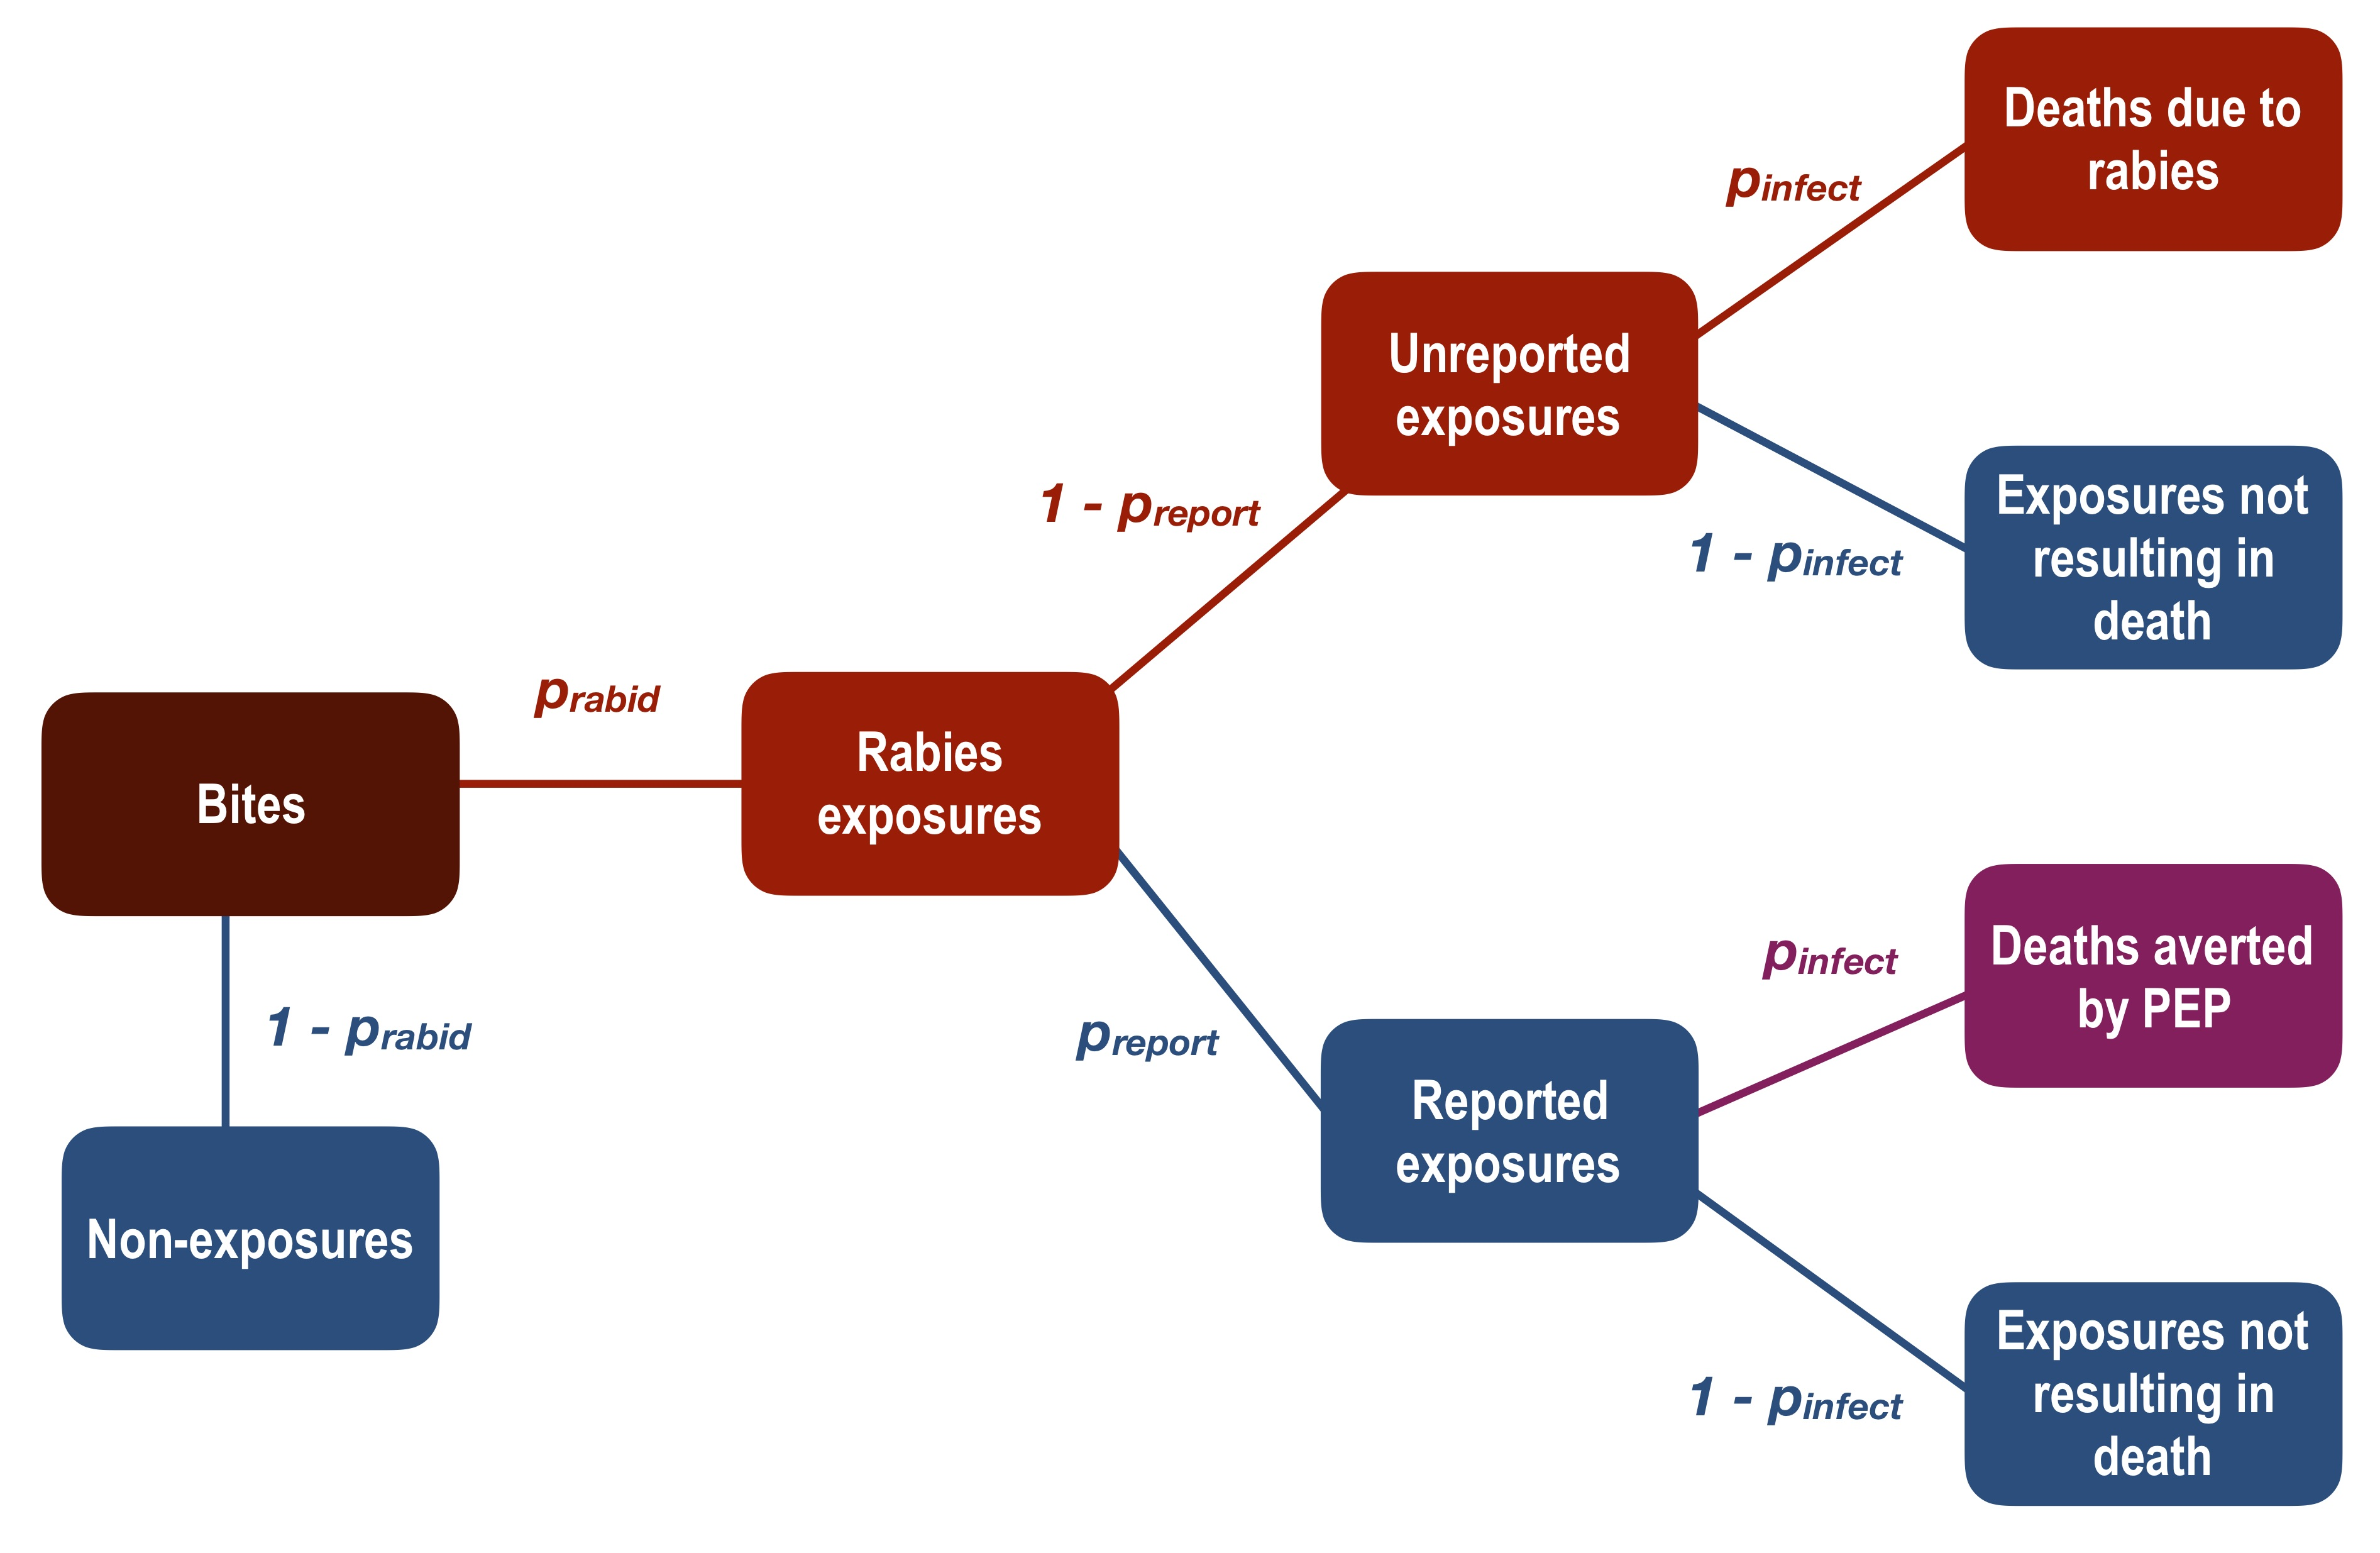
\includegraphics[width=0.95\linewidth]{figs/ch1/fig1} \caption[Adapted decision tree framework to estimate burden of human rabies deaths and deaths averted by PEP.]{Adapted decision tree framework to estimate burden of human rabies deaths and deaths averted by PEP. We considered that some proportion of total bites in the population (expected bites annually, dark red box) are genuine rabies exposures (Bites × \(p_{rabid}\) =Rabies exposures), and non-exposures ((1 − \(p_{rabid}\)) × Bites) do not contribute to rabies deaths or averted deaths. Of the genuine rabies exposures, a fraction present to an ARMC and all of these persons receive PEP (Rabies exposures × \(p_{report}\) = Reported exposures). Some of these exposed persons would otherwise have become infected and died if they had not received PEP (Reported exposures × \(p_{infect}\) = Deaths averted by PEP). Of the unreported exposures, a proportion will die due to rabies infection (Unreported exposures × \(p_{infect}\) = Deaths due to rabies).}\label{fig:fig1}
\end{figure}



\hypertarget{ethics-statement}{%
\subsection{Ethics statement}\label{ethics-statement}}

This research was approved by the Princeton University IRB (\# 7801) and the Ministry of Public Health Ethics Committee (\# 105-MSANP/CE). Oral informed consent was obtained from all interviewed participants. Sample collection from animal carcasses was approved through the Princeton University Institutional Biosafety Committee (\# 1105-16) and the Animal Use and Care Committee (\# 2079A-16).

\hypertarget{results}{%
\section{Results}\label{results}}

\hypertarget{pep-provisioning-at-the-clinic}{%
\subsection{PEP provisioning at the clinic}\label{pep-provisioning-at-the-clinic}}

Between September 2016--December 2017, a total of 1019 patients reported to the ARMC. Multiple patients were likely to present on a given day, with only 3\% of days where a single patient reported. On average, 7 patients presented per day, but this distribution was skewed with 10 or more patients reporting on 22\% of days, and zero patients on only 7\% of days (Fig \ref{fig:fig2}A). Using the updated TRC regimen, an estimated 1927 vials (of 0.5 mL) were required over the study period given the observed daily throughput of ARMC patients. Current ID administration requires approximately 50\% less vaccine vials compared to an IM regimen (3597 vials) (Fig \ref{fig:fig2}B). Use of the abridged 1-week ID regimen could reduce vial use by 20\% and drawing 5 × 0.1 mL injections per vial rather than 4 would further reduce vial use by up to 31\%. In general, extracting 5 × 0.1 mL injections from a vial reduces the volume of vaccine wasted by 40--50\% (Fig \ref{fig:fig2}B).

\begin{figure}
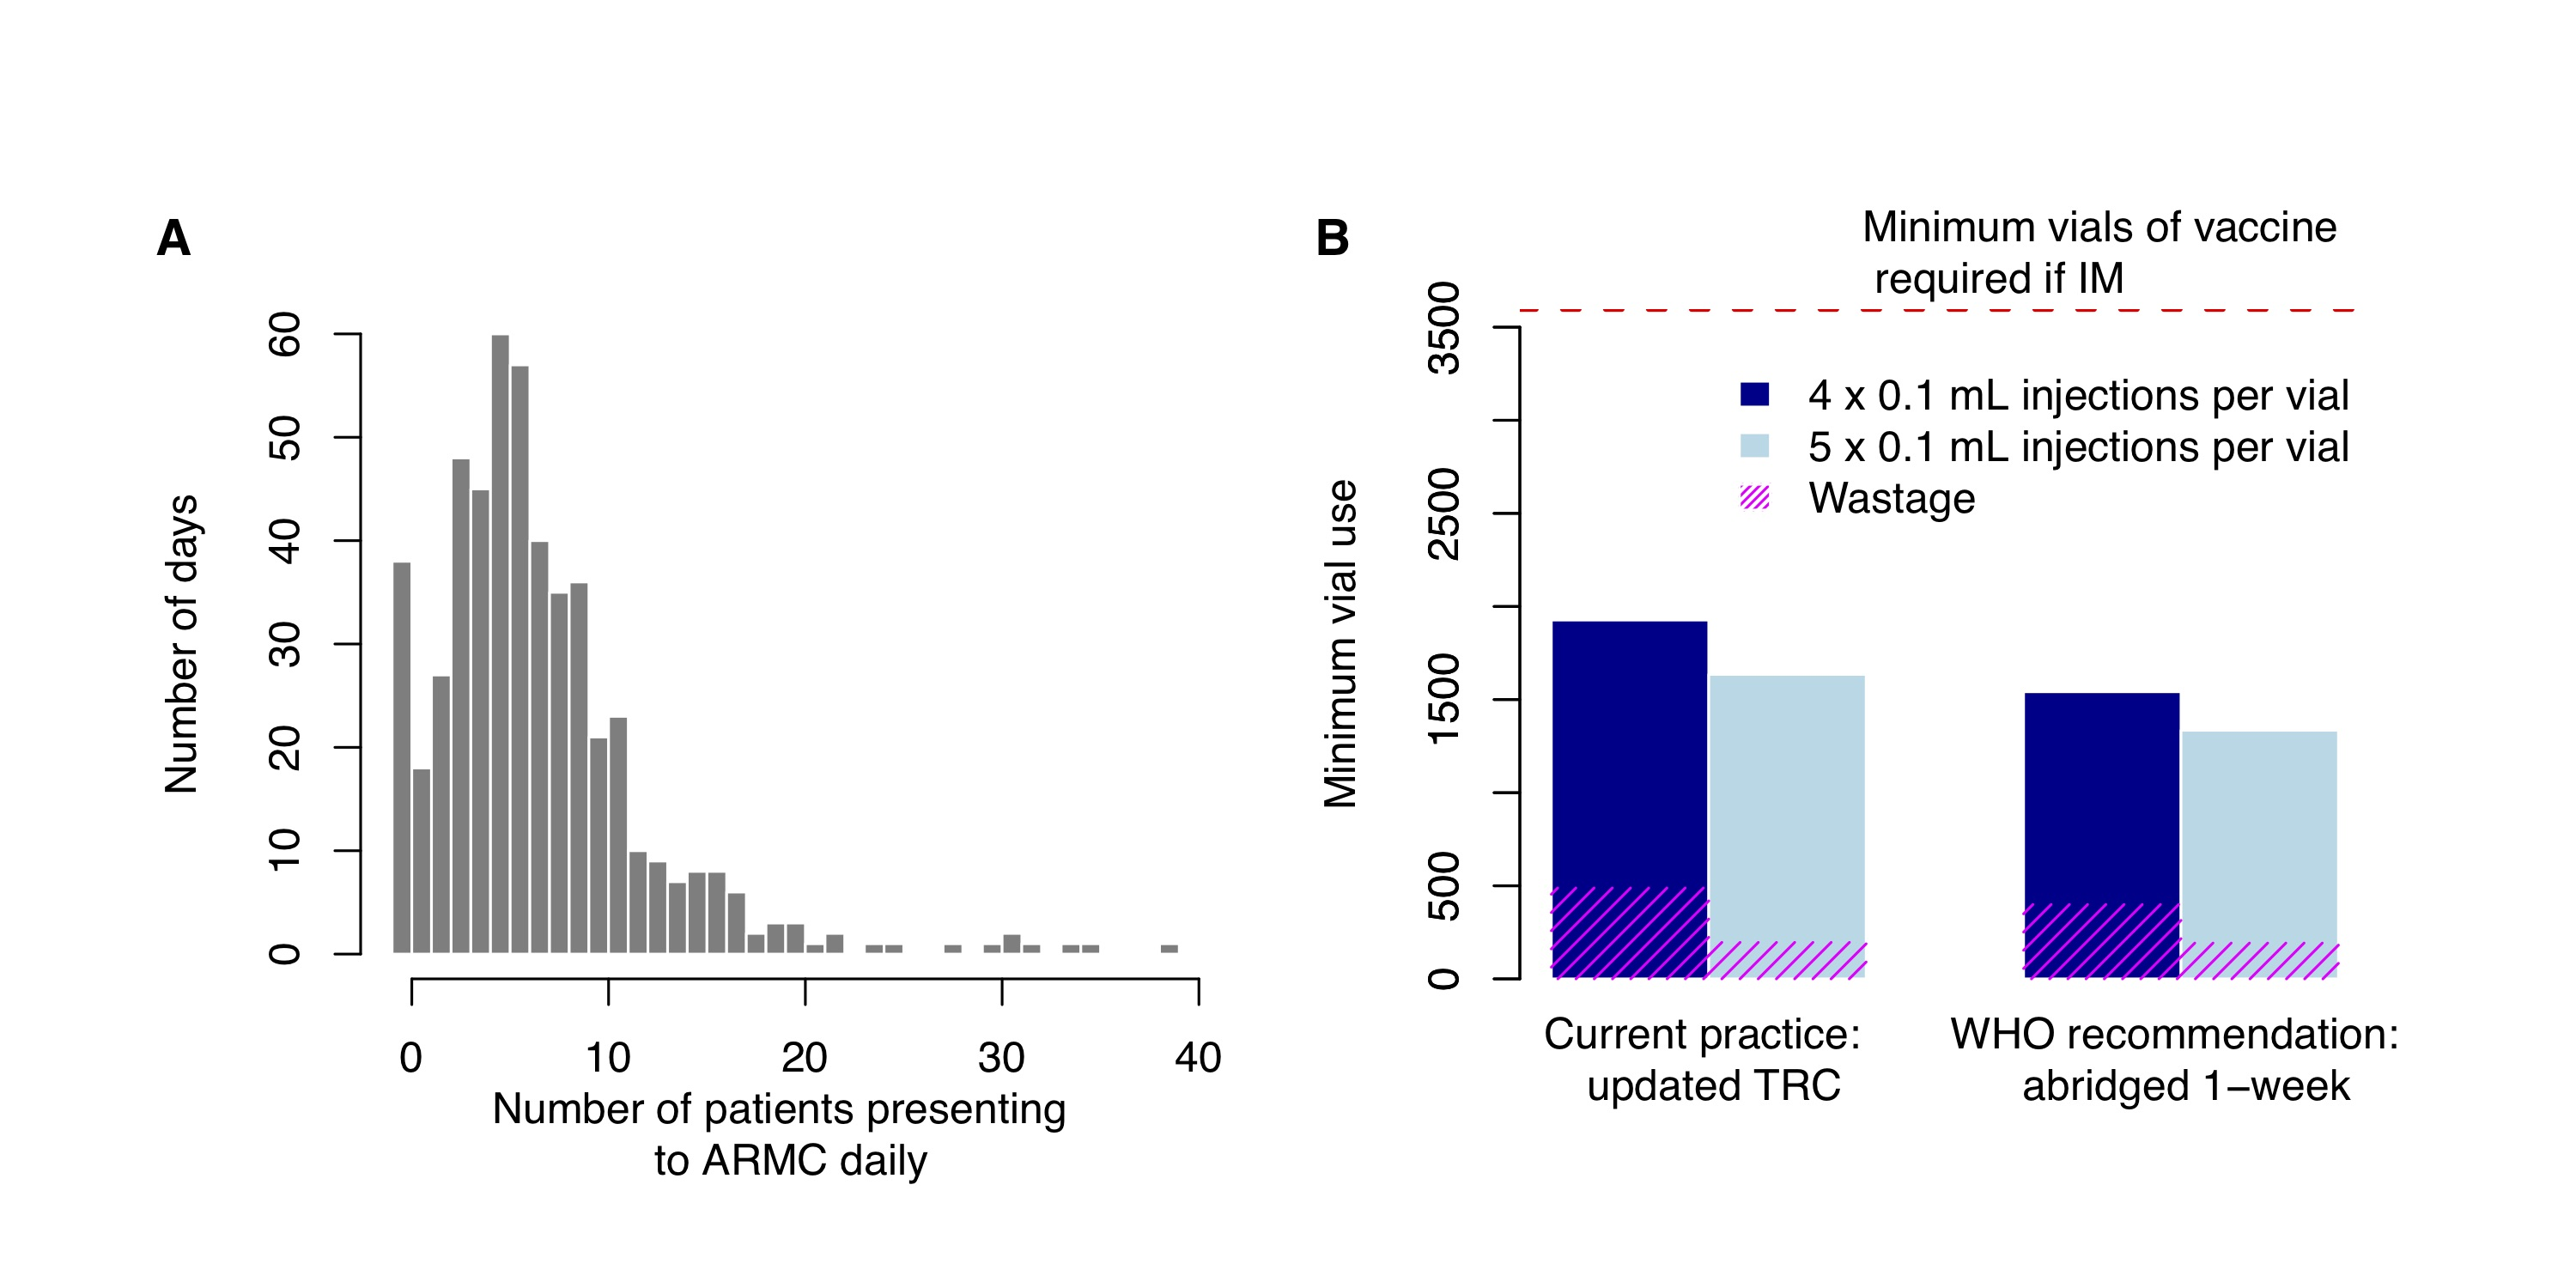
\includegraphics[width=0.95\linewidth]{figs/ch1/fig2} \caption[PEP administration and vaccine use at the Moramanga ARMC.]{PEP administration and vaccine use. (A) Distribution of observed daily patient presentations (i.e.~the number of days with N patients reporting to the ARMC) and (B) calculation of the minimum volume of vaccine (mL) used under current practice with PEP administered according to the updated TRC regimen or according to the latest WHO recommendations with the abridged 1-week ID regimen. Use of 4 × 0.1 mL per 0.5 mL vial (current practice) vs.~5 × 0.1 mL injections per 0.5 mL vial were also compared. The red dashed line corresponds to vaccine use under IM administration, assuming 1 vial per IM injection and the same level of compliance (i.e.~under the Essen 4-dose or Zagreb regimen).}\label{fig:fig2}
\end{figure}



\hypertarget{rabies-status-and-characteristics-of-biting-animals}{%
\subsection{Rabies status and characteristics of biting animals}\label{rabies-status-and-characteristics-of-biting-animals}}

Of the 704 biting animals that were identified at the clinic and through contact tracing, domestic dogs made up the majority (87.5\%), followed by cats (9\%). Other species (\textless4\% of biting animals) included cows, rodents, one lemur, and one bat. The majority were owned animals (56.7\%). We followed up on 390/704 of these animals and identified that 67 were probable cases and 19 were confirmed cases, responsible respectively for 88 probable and 32 confirmed human exposures (Table \ref{tab:tab1}, Fig \ref{fig:fig3}). Almost all of these confirmed/probable rabid animals were domestic dogs (76/87). Rabies was widespread, with confirmed/probable cases detected in 14/21 communes in the Moramanga District (Fig \ref{fig:fig3}A). In addition, there was at least one confirmed case in 11/16 months and at least one probable or confirmed case detected in each month of the study. There were also 4 human cases (1 confirmed, 3 probable) reported in the district during this period (Fig \ref{fig:fig3}B).

\begin{longtable}[]{@{}
  >{\raggedright\arraybackslash}p{(\columnwidth - 8\tabcolsep) * \real{0.57}}
  >{\raggedright\arraybackslash}p{(\columnwidth - 8\tabcolsep) * \real{0.12}}
  >{\raggedright\arraybackslash}p{(\columnwidth - 8\tabcolsep) * \real{0.11}}
  >{\raggedright\arraybackslash}p{(\columnwidth - 8\tabcolsep) * \real{0.10}}
  >{\raggedright\arraybackslash}p{(\columnwidth - 8\tabcolsep) * \real{0.11}}@{}}
\caption{\label{tab:tab1} Characteristics of biting animals as recorded from follow-up investigations.}\tabularnewline
\toprule
& Confirmed (\%) & Probable (\%) & Unknown (\%) & Non-case (\%) \\ \addlinespace
\midrule
\endfirsthead
\toprule
& Confirmed (\%) & Probable (\%) & Unknown (\%) & Non-case (\%) \\ \addlinespace
\midrule
\endhead
Total & 19 & 68 & 108 & 195 \\ \addlinespace
Species & & & & \\ \addlinespace
Cat & 3 (15.8) & 2 (2.9) & 9 (8.3) & 21 (10.8) \\ \addlinespace
Dog & 15 (78.9) & 61 (89.7) & 91 (84.3) & 173 (88.7) \\ \addlinespace
Bovine & 1 (5.3) & 5 (7.4) & 0 (0) & 1 (0.5) \\ \addlinespace
Rodent & 0 (0) & 0 (0) & 6 (5.6) & 0 (0) \\ \addlinespace
Owned animal & 16 (84.2) & 42 (61.8) & 30 (27.8) & 189 (96.9) \\ \addlinespace
Vaccinated & 0 (0) & 0 (0) & 9 (8.3) & 57 (29.2) \\ \addlinespace
Veterinary observation & 3 (15.8) & 5 (7.4) & 4 (3.7) & 68 (34.9) \\ \addlinespace
Outcome & & & & \\ \addlinespace
Alive & 0 (0) & 0 (0) & 14 (13) & 186 (95.4) \\ \addlinespace
Disappeared or unknown & 0 (0) & 17 (25) & 81 (75) & 0 (0) \\ \addlinespace
Died due to disease & 4 (21.1) & 19 (27.9) & 0 (0) & 1 (0.5) \\ \addlinespace
Killed after biting a person/animal & 14 (73.7) & 23 (33.8) & 4 (3.7) & 2 (1) \\ \addlinespace
Other cause of death & 0 (0) & 9 (13.2) & 2 (1.9) & 6 (3.1) \\ \addlinespace
Clinical signs & & & & \\ \addlinespace
Bit multiple people & 11 (57.9) & 26 (38.2) & 0 (0) & 10 (5.1) \\ \addlinespace
Bit other animals & 5 (26.3) & 10 (14.7) & 1 (0.9) & 0 (0) \\ \addlinespace
Observed source of infection(i.e.~signs of previous bite/observed bite) & 4 (21.1) & 5 (7.4) & 2 (1.9) & 2 (1) \\ \addlinespace
Unprovoked aggression & 12 (63.2) & 47 (69.1) & 41 (38) & 33 (16.9) \\ \addlinespace
Excess salivation & 6 (31.6) & 14 (20.6) & 3 (2.8) & 2 (1) \\ \addlinespace
Hydrophobia & 1 (5.3) & 1 (1.5) & 0 (0) & 0 (0) \\ \addlinespace
Lethargy & 2 (10.5) & 7 (10.3) & 0 (0) & 0 (0) \\ \addlinespace
Paralysis & 1 (5.3) & 5 (7.4) & 0 (0) & 1 (0.5) \\ \addlinespace
Vocalization & 3 (15.8) & 4 (5.9) & 0 (0) & 1 (0.5) \\ \addlinespace
Restlessness & 3 (15.8) & 0 (0) & 0 (0) & 0 (0) \\ \addlinespace
Hypersexuality & 0 (0) & 0 (0) & 0 (0) & 0 (0) \\ \addlinespace
Running no reason & 4 (21.1) & 7 (10.3) & 0 (0) & 0 (0) \\ \addlinespace
Strange movement & 2 (10.5) & 8 (11.8) & 1 (0.9) & 1 (0.5) \\ \addlinespace
Provoked bite\textsuperscript{1} & 5 (26.3) & 10 (14.7) & 24 (22.2) & 57 (29.2) \\ \addlinespace
Average number of animals bitten & 0.313 & 0.236 & 0.019 & 0 \\ \addlinespace
Average number of humans bitten & 2.06 & 1.73 & 1 & 1.05 \\ \addlinespace
\bottomrule
\end{longtable}

\emph{\textsuperscript{1}With at least one indication of provocation (i.e.~hitting or kicking the animal, interaction with food or object, playing or running, entering the house of the owner with a guard dog, history of habitual aggression).}

\begin{figure}
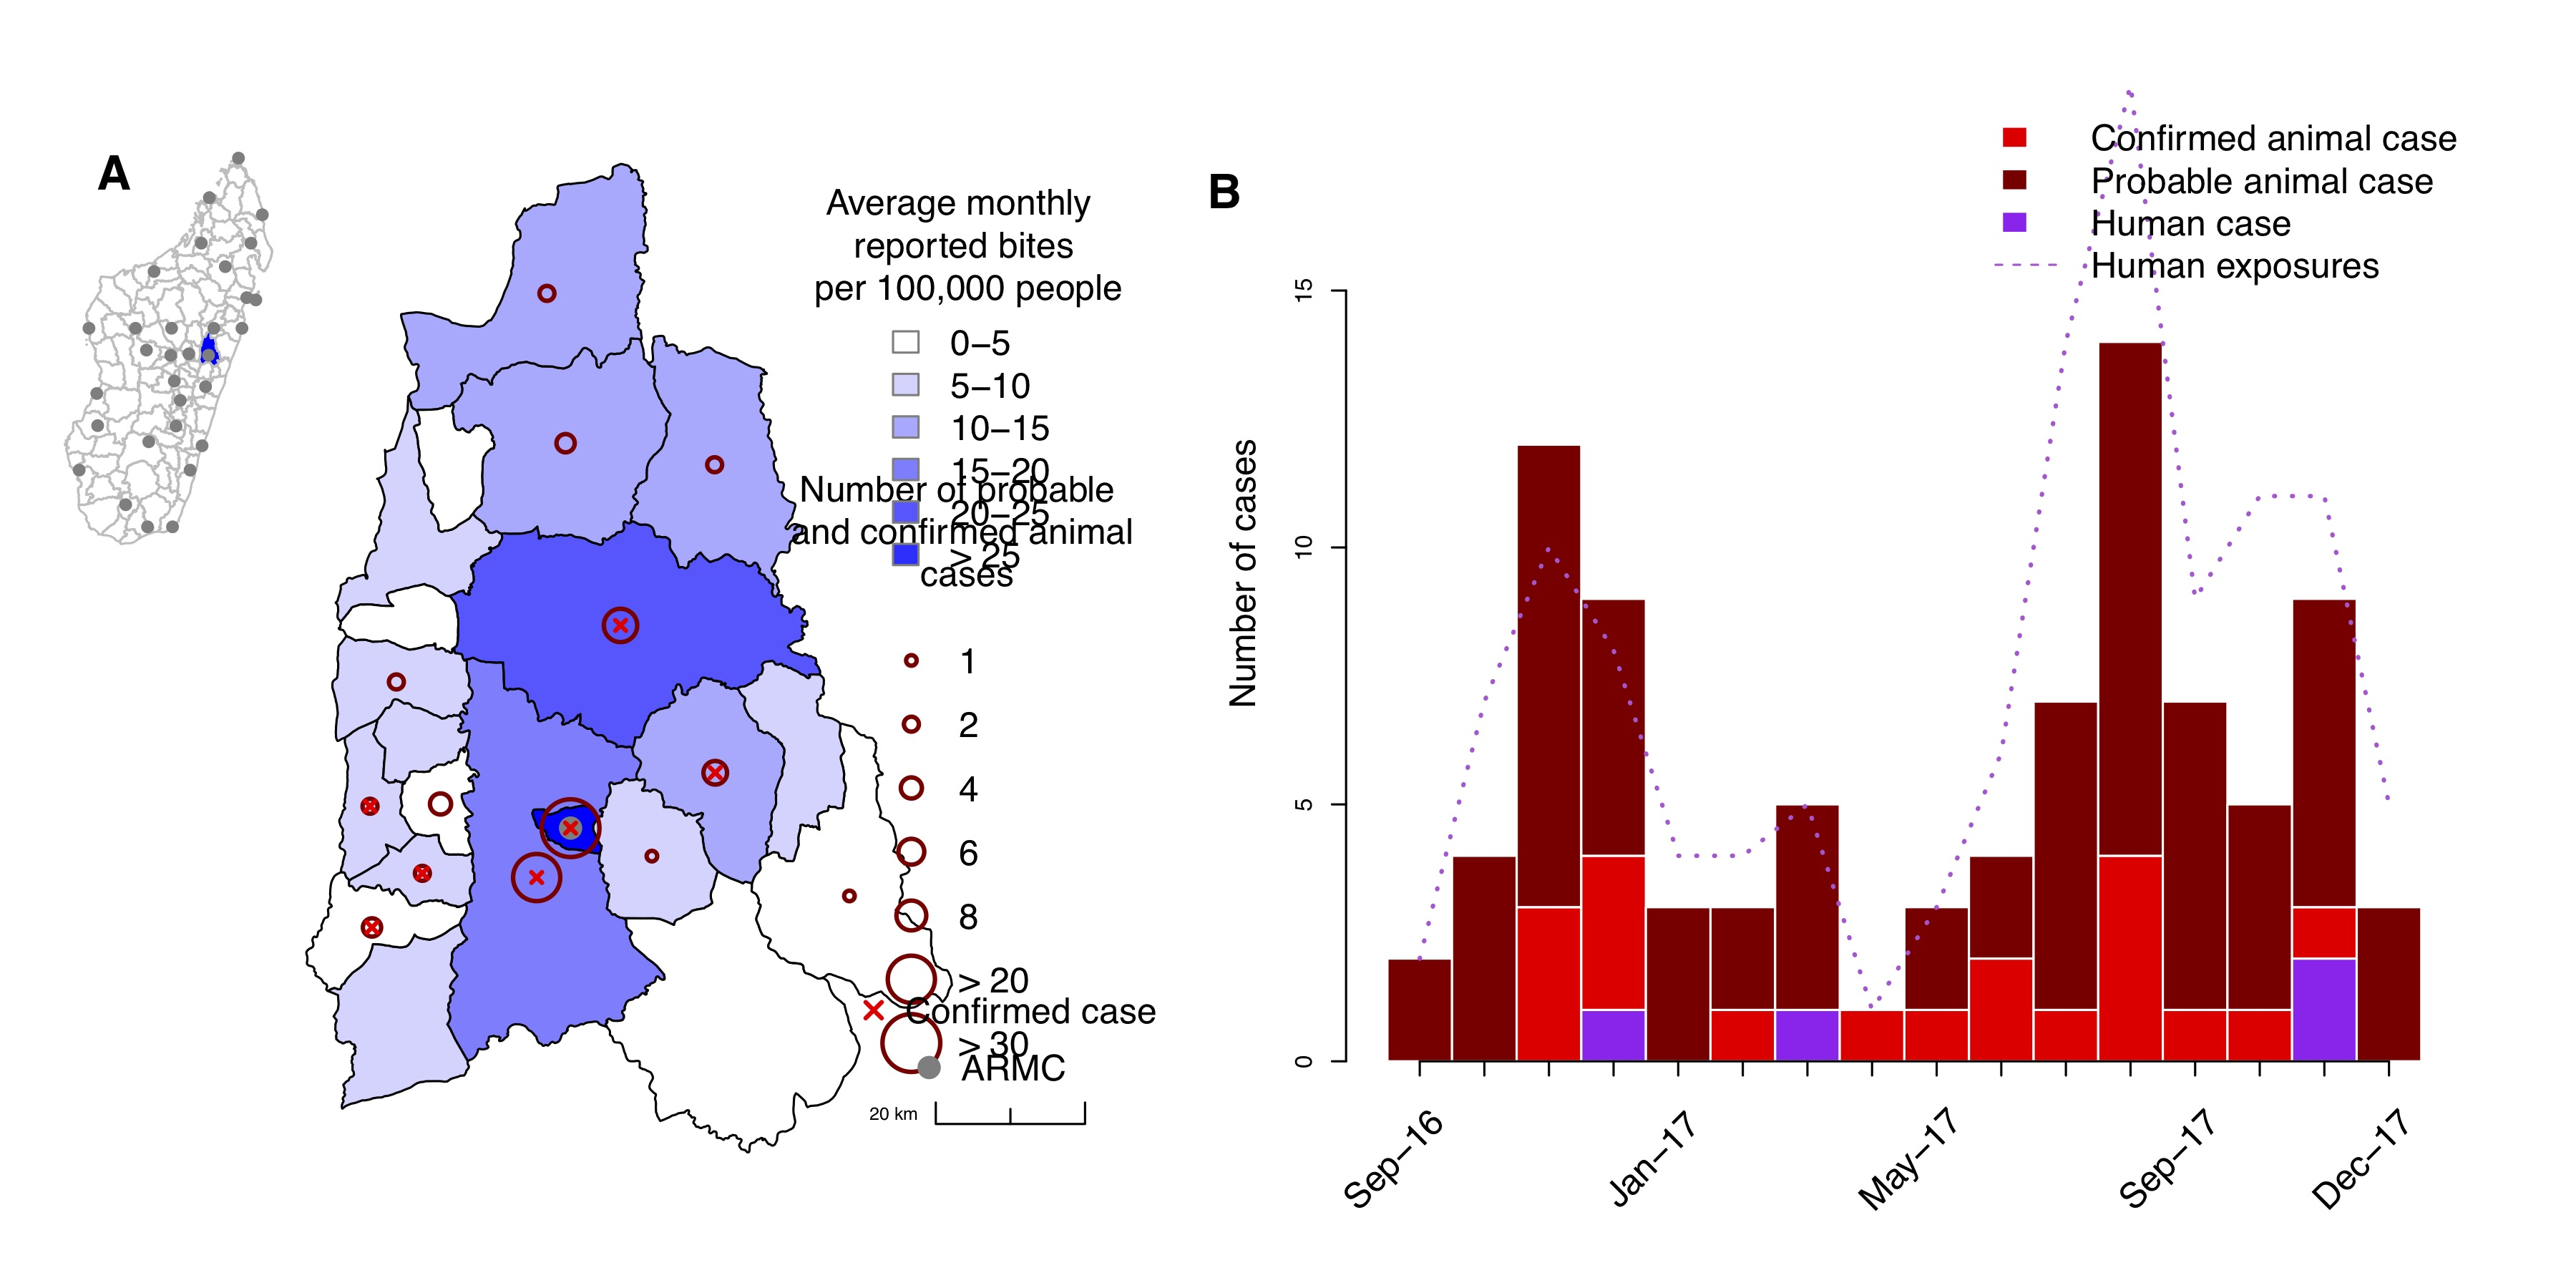
\includegraphics[width=0.95\linewidth]{figs/ch1/fig3} \caption[Spatial and temporal distribution of probable and confirmed animal rabies cases, human exposures, and human deaths in the Moramanga District.]{Rabies in the Moramanga District. (A) Average monthly reported bite incidence (blue shading) per commune and total numbers of probable or confirmed cases (dark red circles). A red × indicates if at least one animal case was confirmed in the commune. All coordinates are the commune centroid, and the inset shows the district (in blue) in relation to the other districts (polygons) and ARMC (grey points) in Madagascar. (B) Time series of probable and confirmed animal cases and human cases (bars), as well as total confirmed/probable rabies exposures (dashed line) from September 2016 to December 2017.}\label{fig:fig3}
\end{figure}



Among probable and confirmed animal rabies cases, unprovoked aggression was the most common clinical sign followed by excessive salivation; other clinical signs were observed less frequently (\textless15\% of probable/confirmed cases). Confirmed and probable animal cases were more frequently involved in biting multiple people (42.5\%) than non-cases (5.4\%). They also more frequently bit several animals. In contrast, provoked bites were twice as common among non-cases (Table \ref{tab:tab1}). Generally, clinical signs were noted for both non-cases and probable cases, and bites from a probable animal could also be classified as provoked based on our criteria (so could not be used to rule out rabies). A source of infection was only identified for nine confirmed or probable cases (i.e.~either an observed bite or signs of a bite prior to biting or the onset of clinical signs). Owners or community members rarely observed when rabid animals bit other animals.

Most probable or confirmed rabid animals were killed after biting or attempting to bite people or other animals (42.5\%), or died from disease (26.4\%) or other causes (10.3\%, including being hit by car, poisoned, or dying from injuries). The remaining 18.6\% disappeared after the bite. The majority of animals classified as non-cases were alive 10 days after the bite (94.4\%), but three animals that were not alive within 10 days of the bite subsequently tested negative, and eight died at a later date (\textgreater10 days after the bite, Table \ref{tab:tab1}).

Of the animals we investigated, 20.5\% were reported to have been placed in veterinary observation. Seven of these 80 observed animals were considered to be probable rabies cases by the veterinarian. However, we did encounter two cases where the veterinary conclusion differed from our case determination (one probable case that was declared a non-case by the veterinary officer due to the age of the animal, i.e.~\textless3 months, and the other that was alive at the time of our investigation approximately 3 months after the bite case, which was declared a suspected rabies case by the veterinary officer at the time of the visit). 17\% of the animals we investigated were reported to be vaccinated, with 29.2\% of non-cases and 28.7\% of those placed in veterinary observation reported to be vaccinated. No probable or confirmed animals had a history of vaccination.

\hypertarget{exposure-status-health-seeking-behavior-and-pep-compliance-of-bite-victims-and-patients-reporting-to-the-armc}{%
\subsection{Exposure status, health-seeking behavior, and PEP compliance of bite victims and patients reporting to the ARMC}\label{exposure-status-health-seeking-behavior-and-pep-compliance-of-bite-victims-and-patients-reporting-to-the-armc}}

Of the 1019 patients presenting to Moramanga AMRC, 1.5\% were in transit and only completed a subset of doses at the clinic. A further 6.8\% came from outside of the district but completed their PEP course in Moramanga; these mostly came from the neighboring district of Anosibe An'Ala (41/63), which does not have an ARMC and is a minimum of 12h travel time from the Moramanga ARMC. Twelve patients were bitten outside the District, but resided in Moramanga and completed their PEP course at the ARMC. We excluded patients bitten in other districts from further analyses.

Excluding contacts with a confirmed/probable case (N = 197), we were able to classify the status of 41.1\% of human exposures over this 16 month period, however this proportion varied over time. By conducting clinic-based triage, we were able to classify double the proportion of bite patients to a known exposure status (27.4\% of patients pre-August 2017 vs.~61.4\% post-August 2017, Fig \ref{fig:fig4}A). Of the 399 patients we followed up with, we were unable to assign an exposure status to 25.8\% (i.e.~`Unknown').

\begin{figure}
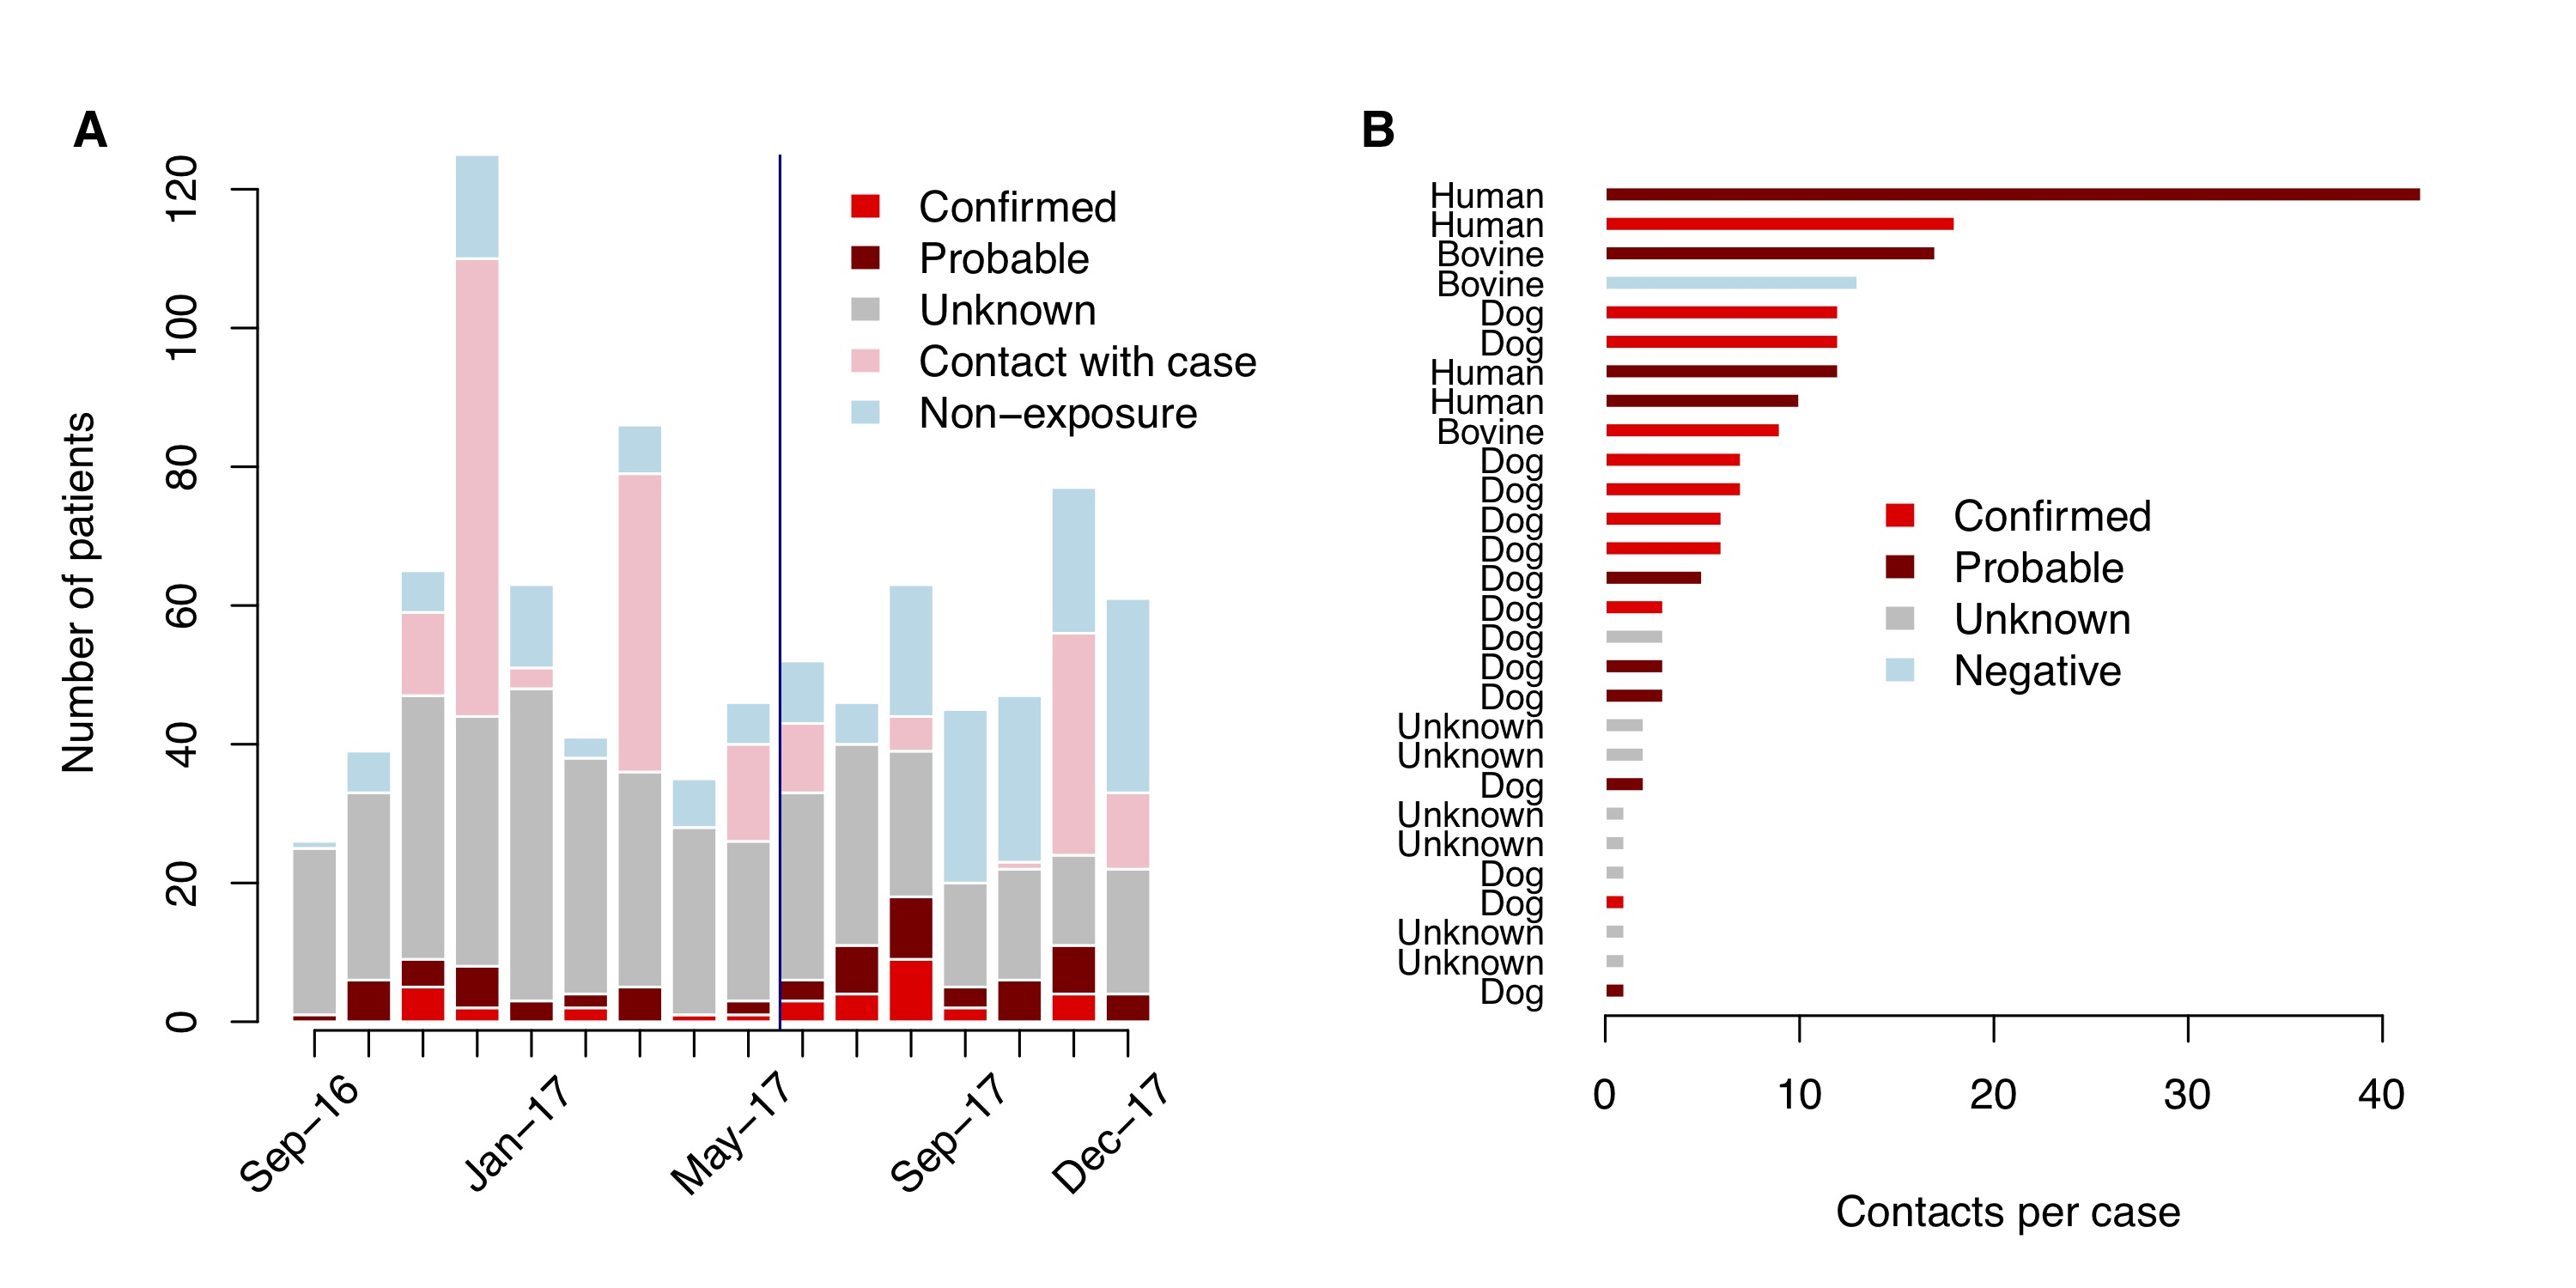
\includegraphics[width=0.95\linewidth]{figs/ch1/fig4} \caption[Time series of patients reporting to the ARMC and clustering of Category I contacts.]{Patients reporting to the ARMC. (A) Monthly time series of patients reporting to the ARMC by their exposure status; the blue line indicates when systematic triaging of patients at the clinic began. (B) Number of contacts per probable case and the rabies status of the case (one bovine case tested negative after sample submission).}\label{fig:fig4}
\end{figure}



Reporting delays were on average 2.8 days for probable exposures and 1.5 days for confirmed exposures, with 61.1\% of patients reporting within 2 days of the exposure overall (Table \ref{tab:tab2}). Overall PEP completion was high, with 89.7\% of patients completing at least 3 doses (88.1\% of probable or confirmed rabies exposures). Approximately 1.7\% of patients completed more than 4 doses, as clinic protocol was to restart the course if there was a delay between PEP doses. Eighteen patients from the Moramanga District were recorded at IPM, and fourteen of these patients received RIG (4 confirmed, 3 unknown, and 7 non-exposures).

\begin{longtable}[]{@{}
  >{\raggedright\arraybackslash}p{(\columnwidth - 10\tabcolsep) * \real{0.45}}
  >{\raggedright\arraybackslash}p{(\columnwidth - 10\tabcolsep) * \real{0.11}}
  >{\raggedright\arraybackslash}p{(\columnwidth - 10\tabcolsep) * \real{0.11}}
  >{\raggedright\arraybackslash}p{(\columnwidth - 10\tabcolsep) * \real{0.10}}
  >{\raggedright\arraybackslash}p{(\columnwidth - 10\tabcolsep) * \real{0.14}}
  >{\raggedright\arraybackslash}p{(\columnwidth - 10\tabcolsep) * \real{0.10}}@{}}
\caption{\label{tab:tab2} Characteristics of all patients reporting for PEP and additional bite victims identified through contact tracing, including the type of exposure and health seeking behavior.}\tabularnewline
\toprule
& Confirmed (\%) & Probable (\%) & Unknown (\%) & Non-exposure (\%) & Contact (\%) \\ \addlinespace
\midrule
\endfirsthead
\toprule
& Confirmed (\%) & Probable (\%) & Unknown (\%) & Non-exposure (\%) & Contact (\%) \\ \addlinespace
\midrule
\endhead
Total & 35 & 85 & 425 & 202 & 197 \\ \addlinespace
Average age & 23.5 & 23.8 & 23.7 & 25.5 & 30.7 \\ \addlinespace
Male & 27 (77.1) & 50 (58.8) & 250 (58.8) & 106 (52.5) & 125 (63.5) \\ \addlinespace
15 yrs or younger & 19 (54.3) & 39 (45.9) & 189 (44.5) & 84 (41.6) & 46 (23.4) \\ \addlinespace
Unreported & 2 (5.7) & 17 (20.0) & 1 (0.2) & 7 (3.5) & -- \\ \addlinespace
Total reported & 33 & 68 & 424 & 195 & 197 \\ \addlinespace
Completing at least 3 doses & 29 (87.9) & 63 (92.6) & 383 (90.3) & 170 (87.2) & 178 (90.4) \\ \addlinespace
Completing at least 4 doses & 29 (87.9) & 56 (82.4) & 316 (74.5) & 129 (66.2) & 157 (79.7) \\ \addlinespace
Completing more than 4 doses & 1 (3) & 3 (4.4) & 8 (1.9) & 3 (1.5) & 1 (0.5) \\ \addlinespace
Average delay between exposure and reporting (days) & 1.5 & 2.8 & 2.6 & 1.8 & NA \\ \addlinespace
Reported within 2 days of bite & 28 (84.8) & 48 (70.6) & 324 (76.4) & 159 (81.5) & -- \\ \addlinespace
Interviewed & 35 (100) & 82 (96.5) & 111 (26.1) & 171 (84.7) & -- \\ \addlinespace
Reported to peripheral clinic before reporting to the ARMC & 0 (0) & 6 (7.3) & 15 (13.5) & 21 (12.3) & -- \\ \addlinespace
Reported to a peripheral clinic only (unreported to ARMC) & 0 (0) & 7 (8.5) & 0 (0) & 3 (1.8) & -- \\ \addlinespace
Reported to any other hospital & 0 (0) & 13 (15.9) & 15 (13.5) & 24 (14) & -- \\ \addlinespace
Wound location** & Legs & 8 (22.9) & 31 (37.8) & 51 (45.9) & 79 (46.2) \\ \addlinespace
Feet & 4 (11.4) & 15 (18.3) & 26 (23.4) & 26 (15.2) & -- \\ \addlinespace
Arms & 9 (25.7) & 5 (6.1) & 6 (5.4) & 14 (8.2) & -- \\ \addlinespace
Hands & 8 (22.9) & 23 (28) & 23 (20.7) & 24 (14) & -- \\ \addlinespace
Upper body & 5 (14.3) & 4 (4.9) & 7 (6.3) & 24 (14) & -- \\ \addlinespace
Head or neck & 2 (5.7) & 4 (4.9) & 1 (0.9) & 6 (3.5) & -- \\ \addlinespace
Wound type** & Skin broken & 21 (60) & 57 (69.5) & 92 (82.9) & 126 (73.7) \\ \addlinespace
Superficial & 25 (71.4) & 59 (72) & 94 (84.7) & 134 (78.4) & -- \\ \addlinespace
Deep & 2 (5.7) & 5 (6.1) & 6 (5.4) & 10 (5.8) & -- \\ \addlinespace
Scratch & 8 (22.9) & 15 (18.3) & 18 (16.2) & 32 (18.7) & -- \\ \addlinespace
Bite & 29 (82.9) & 64 (78) & 91 (82) & 144 (84.2) & -- \\ \addlinespace
Multiple & 1 (2.9) & 1 (1.2) & 1 (0.9) & 3 (1.8) & -- \\ \addlinespace
Over clothes & 7 (20) & 9 (11) & 31 (27.9) & 45 (26.3) & -- \\ \addlinespace
Washed wound & 28 (80) & 62 (75.6) & 96 (86.5) & 139 (81.3) & -- \\ \addlinespace
\bottomrule
\end{longtable}

*Bold rows are denominators for subsequent rows. **Categories are not mutually exclusive and were assigned as they applied to each bite victim.

A total of 201 patients reported as contacts with a probable rabies case (human or animal), making up 20\% of patients receiving PEP. Fig \ref{fig:fig4}B shows the distributions of contacts per case, with contacts with the four human cases comprising the majority of these patients (41.6\%). One bovine case, for which the contacts were people that consumed the meat of the animal, subsequently tested negative. In addition, details about the nature and timing of the contact, and for a subset details on the probable animal itself (6 unknown cases), were not recorded at the clinic.

Overall, demographics of patients were skewed male (59.1\%) and 15 years of age or younger (39.9\%), with almost 50\% of probable/confirmed rabies exposures 15 years of age or younger compared to 37\% of the population in that age group in Moramanga (R. Ratovoson, unpublished data from the Health and Demographic Surveillance System (HDSS) in 3 communes of Moramanga district). For interviewed bite victims (N = 399), we also had data on characteristics of the exposure and post-bite response. The majority of wounds were superficial, but with skin broken. Bites to the head or neck and non-superficial bite injuries made up a small fraction of overall exposures (∼9\%), and most wounds were reported to be from bites vs.~scratches. Overall, 81.4\% of interviewed bite victims reported washing the wound with soap and water (Table \ref{tab:tab2}). 13\% of interviewees reported to peripheral clinics before reporting to the ARMC, with 42 of these 52 patients reporting to a peripheral clinic before reporting for PEP at the ARMC and the 10 remaining patients reporting only to a peripheral clinic (i.e.~did not report for PEP).

We identified a total of 27 people that did not seek PEP, 19 of which were confirmed or probable rabies exposures, resulting in four human deaths (details in Table \ref{tab:tab3}). The remaining 23 were identified during contact tracing investigations and were in good health at the time of investigation; nine of these people reported for PEP after the investigation (5 probable, 2 confirmed exposures, 2 non-exposures). Of the 17 people that reported a reason for not seeking PEP, most were due to ignorance/misconceptions about rabies (n = 9, including thinking the animal was too young to be infected with rabies, not thinking a scratch could result in transmission, reliance on traditional medicine, and complete ignorance of PEP/rabies) and lack of funds to travel to the health center (n = 8).

\begin{longtable}[]{@{}
  >{\raggedright\arraybackslash}p{(\columnwidth - 8\tabcolsep) * \real{0.10}}
  >{\raggedright\arraybackslash}p{(\columnwidth - 8\tabcolsep) * \real{0.14}}
  >{\raggedright\arraybackslash}p{(\columnwidth - 8\tabcolsep) * \real{0.17}}
  >{\raggedright\arraybackslash}p{(\columnwidth - 8\tabcolsep) * \real{0.50}}
  >{\raggedright\arraybackslash}p{(\columnwidth - 8\tabcolsep) * \real{0.12}}@{}}
\caption{\label{tab:tab3} Details of the human deaths in the district during the study period.}\tabularnewline
\toprule
Case (Age, Sex) & Type of exposure & Biting animal & Health-seeking and wound response & Time between bite and death \\ \addlinespace
\midrule
\endfirsthead
\toprule
Case (Age, Sex) & Type of exposure & Biting animal & Health-seeking and wound response & Time between bite and death \\ \addlinespace
\midrule
\endhead
Confirmed (3, F) & Superficial scratch to the face & Owned dog, killed after biting & Did not report to the CTAR or any other hospitals; did not wash wound, but applied tambavy (a local plant). & 12 months \\ \addlinespace
Suspected (67, M) & Bite, no details on location & Owned dog, disappeared after the bite & No details but did not report for PEP. & 1 month \\ \addlinespace
Suspected (61, M) & Superficial bite to the hands & Owned dog, killed after biting & Reported to peripheral clinic and was referred to the CTAR, but did not report for PEP; washed wound and applied oil. & 2 months \\ \addlinespace
Suspected (45, M) & Deep bite to the hands & Unknown dog, disappeared after the bite & Reported to peripheral clinic and was referred to the CTAR, but did not report for PEP; washed wound. & 1 year \\ \addlinespace
\bottomrule
\end{longtable}

\hypertarget{deaths-averted-and-current-burden-of-human-rabies}{%
\subsection{Deaths averted and current burden of human rabies}\label{deaths-averted-and-current-burden-of-human-rabies}}

We calculated an overall incidence of 189 bites per 100,000 people annually. Given this bite incidence and other parameters (Table \ref{tab:tab4}), we estimate between 19 and 50 deaths averted by PEP and between 4 and 9 human rabies deaths in the Moramanga district annually. Extrapolating to the population of Madagascar, we estimate a current burden of 282--745 human rabies deaths annually, with PEP averting an additional 1499--3958 human rabies deaths. Overall, we estimate a rabies exposure incidence of 42--110 per 100,000 persons annually.

\begin{longtable}[]{@{}
  >{\raggedright\arraybackslash}p{(\columnwidth - 4\tabcolsep) * \real{0.27}}
  >{\raggedright\arraybackslash}p{(\columnwidth - 4\tabcolsep) * \real{0.1}}
  >{\raggedright\arraybackslash}p{(\columnwidth - 4\tabcolsep) * \real{0.6}}@{}}
\caption{\label{tab:tab4} Parameters for decision tree model (note that exposures exclude contacts with probable cases).}\tabularnewline
\toprule
Parameter & Value & Description \\ \addlinespace
\midrule
\endfirsthead
\toprule
Parameter & Value & Description \\ \addlinespace
\midrule
\endhead
Overall bite incidence per 100,000 people & 189 & 12 x average of monthly bites (both unreported and reported) between Aug and Dec 2017, when systematic triage was in place \\ \addlinespace
Proportion of overall bites due to rabid animals, \(p_{rabid}\) & 0.22--0.58 & The average monthly proportion of probable/confirmed exposures only (lower limit) or probable/confirmed AND unknown exposures (upper limit) between Aug and Dec 2017, when systematic triage was in place. \\ \addlinespace
Proportion of rabies exposures that seek PEP, \(p_{report}\) & 0.84 & The proportion of probable/confirmed exposures which reported to the ARMC \\ \addlinespace
Proportion of rabies exposures that result in infection in the absence of PEP, \(p_{infect}\) & 0.164 & Changalucha et al.~2018 (submitted) {[}12{]} \\ \addlinespace
Moramanga population & 328,000 & Midpoint between World Pop 2015 and 2020 UN adjusted population projections {[}8{]} \\ \addlinespace
Madagascar population & 26,017,000 & Midpoint between World Pop 2015 and 2020 UN adjusted population projections {[}8{]} \\ \addlinespace
\bottomrule
\end{longtable}

\hypertarget{discussion}{%
\section{Discussion}\label{discussion}}

\hypertarget{key-findings}{%
\subsection{Key findings}\label{key-findings}}

Our results demonstrate that canine rabies is widespread in the Moramanga District and results in a high incidence of human exposures. Current free provisioning of PEP to patients is estimated to prevent the majority of deaths resulting from these exposures. Furthermore, clinic practice of ID administration of PEP uses half the vaccine volume compared to IM administration and shows how vial sharing practices can be implemented effectively in an endemic setting in sub-Saharan Africa. Despite these successful practices, canine rabies is still responsible for a significant burden of human deaths and drives high demand for PEP. The substantial costs of procuring and providing free PEP are currently borne by IPM, but would otherwise fall to Madagascar's health system and/or patients potentially leading to more human rabies deaths.

While approximately 20\% of patients reporting for PEP were classified as rabies exposures, an additional 20\% were due to low-to-no risk contacts with confirmed or probable animal and human cases, many of which do not fit the WHO case definition for a rabies exposure {[}13{]}. Vaccination of loosely defined exposures has been reported in Bhutan, as well, where PEP is provided at no-cost to patients {[}15{]}. These practices may jeopardize vaccination of at-risk persons when PEP availability is limited, as occurred during March 2018 when limited vaccine stocks were used to vaccinate 42 contacts around a human case and subsequently resulted in a stock-out at the Moramanga ARMC. Training to ensure that health workers can effectively obtain 5 × 0.1 mL injections from 0.5 mL vaccine vials would also enable more people to be treated with potential to reduce costs and the risk of vaccine shortages. Rabies control in the dog population would reduce the number of rabies exposures and contacts with human and animal rabies cases, and could therefore reduce the demand for PEP by over 40\%.

Six times as many animal cases were laboratory confirmed during our study period than in the previous 16 months (three animal cases confirmed in the district). Given that between 2011 and 2015, an annual average of 60 rabies case were confirmed in the country, our results suggest significant under-reporting of animal rabies both in the Moramanga district and nationally. Through combined clinical and laboratory diagnosis, we were able to determine the rabies status of ∼40\% of biting animals overall and a higher proportion of animals investigated (∼70\%). Clinic-based triage of bite patients doubled the proportion of exposures we were able to classify. While we did not detect many linked animal cases (either source or secondary) through contact tracing as demonstrated previously in Tanzania {[}16{]}, we identified an additional 19 probable/confirmed exposures, 7 of whom reported to the ARMC after the investigation. In Madagascar, when investigations of suspected human and laboratory confirmed animal cases are conducted leads to the provision of PEP to people who have been in contact with these animals or people. However, shifting effort from these case investigations which focus on vaccinating loosely-defined and likely low-risk contacts, towards routine investigations of probable rabid animal bites to identify untreated exposures, could be a more effective response to prevent human deaths while increasing case detection as part of surveillance {[}17{]}, {[}18{]}.

\hypertarget{strengths-and-limitations}{%
\subsection{Strengths and limitations}\label{strengths-and-limitations}}

We did not address the potential misclassification of rabies cases through our investigations. Overall, 86\% of samples from suspected animals were confirmed positive; however, only 22 samples were tested from the district during this period. Increased efforts to laboratory confirm cases could improve confidence in clinical diagnosis. In general, we believe that our case definition for probable rabies was conservative and likely underestimates the true proportion of rabies exposures (see Section 2, case definitions). Moreover, we may have underestimated rabies exposures and overestimated reporting as investigations were initiated only for patients reporting to the ARMC. We likely missed individuals that reported only to peripheral clinics or that did not report at all (that were not linked to other ARMC patients). Bites by vaccinated dogs also appear to be disproportionately represented in the ARMC as unpublished data from a recent vaccination campaign suggests much lower dog vaccination coverage before the campaign was implemented (5\% pre-April 2018, M. Rajeev unpublished data). During our study, only six patients bitten in the Moramanga District reported directly to IPM without referral, the nearest other ARMC, suggesting that most bite victims in the district that seek PEP are captured at the Moramanga ARMC.

We make several further simplifying assumptions in our estimations of rabies burden in the Moramanga District and our extrapolations to Madagascar. We did not incorporate risks due to incomplete or delayed PEP or for severe exposures that did not receive RIG. Since no deaths were reported from patients who received delayed/incomplete PEP, PEP completion was high, and severe exposures (i.e.~deep wounds) uncommon, we believe this will not have introduced major bias. We did not account for vaccine availability and assumed that all patients that reported to the ARMC received PEP. Although the clinic did not experience PEP shortages during our study, in March 2018 the entire country experienced a stock-out, with no vaccine available at the Moramanga ARMC for two weeks. We also assumed uniform rabies incidence and reporting across Madagascar. Given that only 31 of 114 districts have an ARMC, this likely underestimates the burden and overestimates deaths averted. Data from other districts on bite incidence, rabies exposures, health seeking behavior, and PEP adherence and availability would improve our estimates and understanding of rabies risk across Madagascar.

\hypertarget{wider-context}{%
\subsection{Wider context}\label{wider-context}}

The animal and patient characteristics described in our study are similar to most other rabies endemic settings, with domestic dogs responsible for the majority of animal bites and rabies cases {[}19{]}, {[}20{]}, {[}21{]}, rabies exposures disproportionately affecting children under 15 years of age {[}12{]}, {[}22{]}, patient demographics skewed male {[}15{]}, {[}23{]}, {[}24{]}, and high risk exposures (i.e.~deep wounds or bites to the head or neck) generally rare {[}25{]}. Unlike in some other rabies endemic countries, the majority of patients reported washing the wound with soap and water, which can greatly reduce risk of transmission {[}26{]}, {[}27{]}, {[}28{]}, {[}29{]}. Our estimates of incidence of bite patients, rabies exposures, and human rabies deaths were similar to those from a wide range of endemic settings {[}19{]}, {[}21{]}, {[}22{]}, {[}29{]}. This is the first estimate of rabies burden in Madagascar based on data specific to the country and is in line with the previous estimate of burden for Madagascar using data from sub-Saharan Africa {[}1{]}.

A higher proportion of suspect exposures sought (∼85\%) and completed PEP (∼90\%) compared to other regions with endemic rabies, where PEP is only available at a high cost to patients and a lower proportion of rabies exposed persons receive PEP {[}21{]}, {[}22{]}, {[}24{]}, {[}30{]}, {[}31{]}. Few other studies have described health-seeking behavior and PEP adherence in settings where PEP is free; however, in both Bhutan and Phnom Phen in Cambodia where PEP is provided at no charge to patients, approximately 80--90\% receive and complete PEP {[}15{]}, {[}32{]}. Regardless of whether PEP is free, costs to patients (in the case of free PEP, indirect costs) and limited geographical access seem to present the greatest barriers {[}17{]}, {[}22{]}, {[}33{]}. In addition, awareness on the part of both patients and clinicians responsible for referrals also contribute to bite victims not receiving PEP {[}34{]}.

We were able to determine the rabies status for animals we investigated to a comparable level as that reported in similar studies in Haiti and Tanzania {[}20{]}, {[}35{]}. Overall, approximately 20\% of animal bites were determined to be likely rabies exposures compared to 13\% in Haiti {[}20{]}, 73\% in Ethiopia {[}21{]}, and 62\% in Tanzania {[}22{]}. This variation may be due to differences in dog vaccination, as well as higher health seeking of people bitten by non-rabid animals in free settings (higher levels of dog vaccination coverage in Haiti and Tanzania; more costly PEP in Ethiopia and Tanzania). Our results suggest that implementing recently developed integrated bite case management programs which use risk assessments to prioritize PEP administration {[}17{]}, {[}34{]}, {[}36{]} and using bite patients as sentinels for rabies surveillance {[}35{]} are feasible and effective options to better manage PEP and improve surveillance in Madagascar, especially as control in the dog population is implemented.

\hypertarget{conclusions-recommendations}{%
\subsection{Conclusions \& recommendations}\label{conclusions-recommendations}}

Our findings show that canine rabies is responsible for a high incidence of human rabies exposures and preventable rabies deaths in Madagascar, and accounts for a large proportion of the demand for PEP. Given current successful ID administration of PEP and vial sharing practices, adoption of the latest WHO recommendations for PEP administration using the abridged 1-week ID regimen could be implemented immediately in Madagascar to reduce PEP costs. Shifting away from control strategies of reactive culling to mass dog vaccination would further reduce both the high costs of PEP and the burden of human rabies. Increasing access to PEP and awareness for its need could also greatly reduce the burden of human rabies, especially given its limited availability within Madagascar. Nonetheless, the fact that where PEP is available, it is provided to patients for free, appears to result in relatively high health seeking and adherence in comparison to other low-income settings. In general, more judicious use of PEP may be warranted as access is expanded and vaccine use increases. Particularly, if mass dog vaccination is implemented and risk of rabies exposures decrease, integrated bite case management {[}36{]} could be used to further reduce PEP demand while enhancing surveillance of animal cases and identification of exposed persons {[}20{]}, {[}35{]}. However, this would require improved integration of activities and coordination between the health and veterinary sectors. Given the push to eliminate deaths due to human rabies {[}4{]}, our results demonstrate that investing in rabies control as a public good through providing free PEP can prevent needless human deaths, and in combination with mass dog vaccination has the potential to greatly reduce and eventually eliminate rabies from Madagascar.

\hypertarget{acknowledgements}{%
\section{Acknowledgements}\label{acknowledgements}}

We would like to thank all staff and officials at the Moramanga ARMC and other hospitals in the district, the local veterinarians, livestock officers, the local presidents and town officials, and the National Rabies Laboratory who were integral to this work. We are grateful to staff and officials at IPM, the Ministry of Public Health, and the Department of Veterinary Services for their support and technical assistance. In particular, we thank Jean Hyacinthe Randrianarisoa, Ranaivoarimanana, Fierenantsoa Randriamahatana, Esther Noiarisaona, Girard Razafitrimo, Cara Brook, Amy Winter, Christian Ranaivoson, John Friar, and Amy Wesolowski. This work was funded by grants from the Center for Health and Wellbeing and the Department of Ecology and Evolutionary Biology at Princeton University to CJEM and MR. MR is supported by an NSF Graduate Research Fellowship. KH is supported by the Wellcome Trust (207569/Z/17/Z).

\hypertarget{conflict-of-interest-statement}{%
\section{Conflict of interest statement}\label{conflict-of-interest-statement}}

The authors declare no conflicts of interest.

\hypertarget{author-contributions}{%
\section{Author contributions}\label{author-contributions}}

MR, GE, CH, SF, HG, JMH, MA, CJEM, and KH conceived and designed the study. MR, GE, CH, SF, HG, JMH, RR, RR, LR, LB acquired and/or analyzed the data. MR, CJEM, and KH drafted the article. All authors provided critical feedback and approved the final version to be submitted.

\hypertarget{data-availability}{%
\section{Data availability}\label{data-availability}}

Anonymized data are available on request and pending approval of the Ministry of Public Health and IPM.

\hypertarget{references-1}{%
\section{References}\label{references-1}}

\setlength{\parskip}{1em}

{[}1{]} K. Hampson, L. Coudeville, T. Lembo, M. Sambo, A. Kieffer, M. Attlan, et al.~Estimating the global burden of endemic canine rabies. PLoS Negl Trop Dis, 9 (2015), Article e0003709, 10.1371/journal.pntd.0003709

{[}2{]} T. Hemachudha, J. Laothamatas, C.E. Rupprecht. Human rabies: a disease of complex neuropathogenetic mechanisms and diagnostic challenges. Lancet Neur, 1 (2002), pp.~101-109, 10.1016/S1474-4422(02)00041-8

{[}3{]} World Health Organization. WHO Expert Consultation on Rabies. Second report. World Health Organ Tech Rep Ser 2013: 1--139--backcover.

{[}4{]} B. Abela-Ridder, L. Knopf, S. Martin, L. Taylor, G. Torres, K. de Balogh. 2016: the beginning of the end of rabies? Lancet Glob Health (2016), 10.1016/S2214-109X(16)30245-5

{[}5{]} J.-M. Reynes, S.F. Andriamandimby, G.M. Razafitrimo, J. Razainirina, E.M. Jeanmaire, H. Bourhy, et al.~Laboratory surveillance of rabies in humans, domestic animals, and bats in madagascar from 2005 to 2010. Adv Prev Med, 2011 (2011), Article 727821, 10.4061/2011/727821

{[}6{]} S.F. Andriamandimby, J.-M. Heraud, R. Ramiandrasoa, M. Ratsitorahina, J.H. Rasambainarivo, L. Dacheux, et al.~Surveillance and control of rabies in La Reunion, Mayotte, and Madagascar. Vet Res, 44 (2013), p.~77, 10.1186/1297-9716-44-77

{[}7{]} F.S. Rasolonjatovo. Evaluation de l'utilisation du papier buvard pour le diagnostic moléculaire de l'infection par le virus rabique. Thèse De Médecine Vétérinaire Université d'Antananarivo (2017), pp.~1-114

{[}8{]} C. Linard, M. Gilbert, R.W. Snow, A.M. Noor, A.J. Tatem. Population distribution, settlement patterns and accessibility across Africa in 2010. PLoS ONE, 7 (2012), pp.~e31743-e31748, 10.1371/journal.pone.0031743

{[}9{]} F.-X. Meslin, M.M. Kaplan, H. Koprowski. Laboratory techniques in rabies. World Health Organization (1996)

{[}10{]} L. Dacheux, F. Larrous, R. Lavenir, A. Lepelletier, A. Faouzi, C. Troupin, et al.~Dual combined real-time reverse transcription polymerase chain reaction assay for the diagnosis of lyssavirus infection. PLoS Negl Trop Dis, 10 (2016), pp.~e0004812-e4818, 10.1371/journal.pntd.0004812

{[}11{]} V. Tepsumethanon, H. Wilde, F.X. Meslin. Six criteria for rabies diagnosis in living dogs. J Med Assoc Thai, 88 (2005), pp.~419-422

{[}12{]} D.L. Knobel, S. Cleaveland, P.G. Coleman, E.M. Fèvre, M.I. Meltzer, M.E.G. Miranda, et al.~Re-evaluating the burden of rabies in Africa and Asia. Bull World Health Organ, 83 (2005), pp.~360-368

{[}13{]} Rabies vaccines: WHO position paper. WHO Wkly Epidemiol Rec; 2018.

{[}14{]} J. Changalucha, E.A. Mpolya, Z. Mtema. The need to improve access to rabies post-exposure vaccines: lessons from Tanzania. Vaccine, 37 (S1) (2019), pp.~A45-A53

{[}15{]} Dhand NK Tenzin, M.P. Ward. Human rabies post exposure prophylaxis in Bhutan, 2005--2008: trends and risk factors. Vaccine, 29 (2011), pp.~4094-4101, 10.1016/j.vaccine.2011.03.106

{[}16{]} K. Hampson, J. Dushoff, S. Cleaveland, D.T. Haydon, M. Kaare, C. Packer, et al.~Transmission dynamics and prospects for the elimination of canine rabies. PLOS Biol, 7 (2009), Article e53, 10.1371/journal.pbio.1000053

{[}17{]} M.D.~Etheart, M. Kligerman, P.D. Augustin, J.D. Blanton, B. Monroe, L. Fleurinord, et al.~Effect of counselling on health-care-seeking behaviours and rabies vaccination adherence after dog bites in Haiti, 2014â€"15: a retrospective follow-up survey. Lancet Glob Health, 5 (2017), pp.~e1017-e1025, 10.1016/S2214-109X(17)30321-2

{[}18{]} A. Medley, M. Millien, J. Blanton, X. Ma, P. Augustin, K. Crowdis, et al.~Retrospective cohort study to assess the risk of rabies in biting dogs, 2013--2015, Republic of Haiti 14--13. Tropical Med, 2 (2017), 10.3390/tropicalmed2020014

{[}19{]} M.K. Sudarshan, S.N. Madhusudana, B.J. Mahendra, N.S.N. Rao, D.H. Ashwath Narayana, S. Abdul Rahman, et al.~Assessing the burden of human rabies in India: results of a national multi-center epidemiological survey. Int J Infect Dis, 11 (2007), pp.~29-35, 10.1016/j.ijid.2005.10.007

{[}20{]} R.M. Wallace, H. Reses, R. Franka, P. Dilius, N. Fenelon, L. Orciari, et al.~Establishment of a canine rabies burden in haiti through the implementation of a novel surveillance program. PLoS Negl Trop Dis, 9 (2015), pp.~e0004245-e4315, 10.1371/journal.pntd.0004245

{[}21{]} T.J. Beyene, M.C.M. Mourits, A.H. Kidane, H. Hogeveen. Estimating the burden of rabies in Ethiopia by tracing dog bite victims. PLoS ONE, 13 (2018), Article e0192313, 10.1371/journal.pone.0192313

{[}22{]} K. Hampson, A. Dobson, M. Kaare, J. Dushoff, M. Magoto, E. Sindoya, et al.~Rabies exposures, post-exposure prophylaxis and deaths in a region of endemic canine rabies. PLoS Negl Trop Dis, 2 (2008), pp.~1-9, 10.1371/journal.pntd.0000339

{[}23{]} N.J. Gogtay, A. Nagpal, A. Mallad, K. Patel, S.J. Stimpson, A. Belur, et al.~Demographics of animal bite victims \& management practices in a tertiary care institute in Mumbai, Maharashtra, India. Indian J Med Res, 139 (2014), pp.~459-462

{[}24{]} J. Frey, R. Mindekem, H. Kessely, D.D. Moto, S. Naissengar, J. Zinsstag, et al.~Survey of animal bite injuries and their management for an estimate of human rabies deaths in N'Djaména, Chad. Trop Med Int Health, 18 (2013), pp.~1555-1562, 10.1111/tmi.12202

{[}25{]} V. Tricou, J. Bouscaillou, E. Kamba Mebourou, F.D. Koyanongo, E. Nakouné, M. Kazanji. Surveillance of canine rabies in the Central African Republic: impact on human health and molecular epidemiology. PLoS Negl Trop Dis, 10 (2016), pp.~e0004433-e4517, 10.1371/journal.pntd.0004433

{[}26{]} M. Sambo, T. Lembo, S. Cleaveland, H.M. Ferguson, L. Sikana, C. Simon, et al.~Knowledge, attitudes and practices (KAP) about rabies prevention and control: a community survey in Tanzania. PLoS Negl Trop Dis, 8 (2014), pp.~e3310-e3311, 10.1371/journal.pntd.0003310

{[}27{]} R. Tschopp, S. Bekele, A. Aseffa. Dog demography, animal bite management and rabies knowledge-attitude and practices in the awash basin, Eastern Ethiopia. PLoS Negl Trop Dis, 10 (2016), pp.~e0004471-e4514, 10.1371/journal.pntd.0004471

{[}28{]} C. Mbilo, M. Léchenne, J. Hattendorf, S. Madjadinan, F. Anyiam, J. Zinsstag. Rabies awareness and dog ownership among rural northern and southern Chadian communities-analysis of a community-based, cross-sectional household survey. Acta Trop (2016), 10.1016/j.actatropica.2016.06.003

{[}29{]} Dhand NK Tenzin, T. Gyeltshen, S. Firestone, C. Zangmo, C. Dema, et al.~Dog bites in humans and estimating human rabies mortality in rabies endemic areas of bhutan. PLoS Negl Trop Dis, 5 (2011), Article e1391, 10.1371/journal.pntd.0001391

{[}30{]} A.S. Youla, F.A. Traore, F.B. Sako, R.M. Feda, M.A.~Emeric. Canine and human rabies in Conakry: epidemiology and preventive aspects. Bull Soc Pathol Exot, 107 (2013), pp.~18-21, 10.1007/s13149-013-0321-x

{[}31{]} C. Salomão, A. Nacima, L. Cuamba, L. Gujral, O. Amiel, C. Baltazar, et al.~Epidemiology, clinical features and risk factors for human rabies and animal bites during an outbreak of rabies in Maputo and Matola cities, Mozambique, 2014: implications for public health interventions for rabies control. PLoS Negl Trop Dis, 11 (2017), pp.~e0005787-e5816, 10.1371/journal.pntd.0005787

{[}32{]} S. Ly, P. Buchy, N.Y. Heng, S. Ong, N. Chhor, H. Bourhy, et al.~Rabies situation in Cambodia. PLoS NeglTrop Dis (2009), 10.1371/journal.pntd.0000511

{[}33{]} A. Tarantola, S. Blanchi, J. Cappelle, S. Ly, M. Chan, S. In, et al.~Rabies postexposure prophylaxis noncompletion after dog bites: estimating the unseen to meet the needs of the underserved. Am J Epidemiol, 101 (2017), pp.~765-810, 10.1093/aje/kwx234

{[}34{]} M. Léchenne, R. Mindekem, S. Madjadinan, A. Oussiguere, D.D. Moto, K. Naissengar, et al.~The importance of a participatory and integrated one health approach for rabies control: the case of N'Djaména, Chad 43--16. Tropical Med, 2 (2017), 10.3390/tropicalmed2030043

{[}35{]} Hampson K, Abela-Ridder B, Brunker K, Bucheli STM, Carvalho M, Caldas E, et al.~Surveillance to Establish Elimination of Transmission and Freedom from Dog-mediated Rabies. bioRxiv 2016: 096883. \url{https://doi.org/10.1101/096883}.

{[}36{]} E.A. Undurraga, M.I. Meltzer, C.H. Tran, C.Y. Atkins, M.D.~Etheart, M.F. Millien, et al.~Cost-effectiveness evaluation of a novel integrated bite case management program for the control of human rabies, Haiti 2014--2015. Am J Trop Med Hyg, 96 (2017), pp.~1307-1317, 10.4269/ajtmh.16-0785

\hypertarget{how-geographic-access-to-care-shapes-disease-burden-the-current-impact-of-post-exposure-prophylaxis-and-potential-for-expanded-access-to-prevent-human-rabies-deaths-in-madagascar}{%
\chapter{How geographic access to care shapes disease burden: the current impact of post-exposure prophylaxis and potential for expanded access to prevent human rabies deaths in Madagascar}\label{how-geographic-access-to-care-shapes-disease-burden-the-current-impact-of-post-exposure-prophylaxis-and-potential-for-expanded-access-to-prevent-human-rabies-deaths-in-madagascar}}

\emph{This chapter will be published in:}

\emph{\textbf{Rajeev, M.} Guis, H., Edosoa G., Hanitriniaina, C., Andriamandimby, S.F., Randrianarijaona A., Mangahasimbola, RT, Ramiandrasoa, R., Baril, L., Metcalf, C.J.E, \& Hampson, K. (2020). How geographic access to care shapes disease burden: the current impact of post-exposure prophylaxis and potential for expanded access to prevent human rabies deaths in Madagascar. medRxiv: 10.02.20205948. Accepted at PLoS NTD.}

\emph{Minor formatting modifications and edits have been made for the dissertation.}

\newpage
\setlength{\parskip}{2em}

\hypertarget{abstract-1}{%
\section*{Abstract}\label{abstract-1}}
\addcontentsline{toc}{section}{Abstract}

\hypertarget{background}{%
\subsection*{Background}\label{background}}
\addcontentsline{toc}{subsection}{Background}

Post-exposure prophylaxis (PEP) is highly effective at preventing human
rabies deaths, however access to PEP is limited in many rabies endemic
countries. The 2018 decision by Gavi to add human rabies vaccine to its
investment portfolio should expand PEP availability and reduce rabies
deaths. We explore how geographic access to PEP impacts the rabies
burden in Madagascar and the potential benefits of improved
provisioning.

\hypertarget{methodology-principal-findings}{%
\subsection*{Methodology \& Principal Findings}\label{methodology-principal-findings}}
\addcontentsline{toc}{subsection}{Methodology \& Principal Findings}

We use spatially resolved data on numbers of bite patients seeking PEP
across Madagascar and estimates of travel times to the closest clinic
providing PEP (N = 31) in a Bayesian regression framework to estimate
how geographic access predicts reported bite incidence. We find that
travel times strongly predict reported bite incidence across the
country. Using resulting estimates in an adapted decision tree, we
extrapolate rabies deaths and reporting and find that geographic access
to PEP shapes burden sub-nationally. We estimate 960 human rabies deaths
annually (95\% Prediction Intervals (PI):790 - 1120), with PEP averting
an additional 800 deaths (95\% PI: 800 (95\% PI: 640 - 970) each year.
Under these assumptions, we find that expanding PEP to one clinic per
district (83 additional clinics) could reduce deaths by 19\%, but even
with all major primary clinics provisioning PEP (1733 additional
clinics), we still expect substantial rabies mortality. Our quantitative
estimates are most sensitive to assumptions of underlying rabies
exposure incidence, but qualitative patterns of the impacts of travel
times and expanded PEP access are robust.

\hypertarget{conclusions-significance}{%
\subsection*{Conclusions \& Significance}\label{conclusions-significance}}
\addcontentsline{toc}{subsection}{Conclusions \& Significance}

PEP is effective at preventing rabies deaths, and in the absence of
strong surveillance, targeting underserved populations may be the most
equitable way to provision PEP. Given the potential for countries to use
Gavi funding to expand access to PEP in the coming years, this framework
could be used as a first step to guide expansion and improve targeting
of interventions in similar endemic settings where PEP access is
geographically restricted and baseline data on rabies risk is lacking.
While better PEP access should save many lives, improved outreach,
surveillance, and dog vaccination will be necessary, and if rolled out
with Gavi investment, could catalyze progress towards achieving zero
rabies deaths.

\hypertarget{author-summary}{%
\section*{Author Summary}\label{author-summary}}
\addcontentsline{toc}{section}{Author Summary}

Canine rabies causes an estimated 60,000 deaths each year across the
world, primarily in low- and middle-income countries where people have
limited access to both human vaccines (post-exposure prophylaxis or PEP)
and dog rabies vaccines. Given that we have the tools to prevent rabies
deaths, a global target has been set to eliminate deaths due to canine
rabies by 2030, and recently, Gavi, a multilateral organization that
aims to improve access to vaccines in the poorest countries, added human
rabies vaccine to it's portfolio. In this study, we estimated reported
incidence of patients seeking PEP in relation to travel times to clinics
provisioning PEP and extrapolate human rabies deaths in Madagascar. We
find that PEP currently averts around 800 deaths each year, but that the
burden remains high (1000 deaths/ year), particularly in remote,
hard-to-reach areas. We show that expanding PEP availability to more
clinics could significantly reduce rabies deaths in Madagascar, but our
results reaffirm that expansion alone is will not achieve the global
goal of zero human deaths from dog-mediated rabies by 2030. Combining
PEP expansion with outreach, surveillance, and mass dog vaccination
programs will be necessary to move Madagascar, and other Low- and
Middle-Income countries, forward on the path to rabies elimination.

\hypertarget{introduction-2}{%
\section{Introduction}\label{introduction-2}}

Inequities in access to care are a major driver of disease burden
globally {[}1{]}. Often, the populations at greatest risk of a given
disease are the most underserved {[}2{]}. Delivering interventions to
these groups is challenging due to financial and infrastructural
limitations and requires careful consideration of how best to allocate
limited resources {[}3{]}.

Canine rabies is estimated to cause approximately 60,000 human deaths
annually {[}4{]}. Mass vaccination of domestic dogs has been demonstrated
to be a highly effective way to control the disease in both animals and
humans. While dog vaccination can interrupt transmission in the
reservoir, human deaths can also be prevented through prompt
administration of post-exposure prophylactic vaccines (PEP) following a
bite by a rabid animal {[}5{]}. However, access to the human rabies
vaccine is limited in many countries where canine rabies is endemic
{[}6--8{]}, and within countries these deaths are often concentrated in
rural, underserved communities {[}9{]}.

In 2015, a global framework to eliminate deaths due to canine rabies by
2030 (`Zero by 30') through a combination of PEP provisioning and dog
vaccination was established by the World Health Organization (WHO) and
partners {[}10{]}. Furthermore, in 2018, Gavi, the Vaccine Alliance, added
human rabies vaccines to their proposed investment portfolio {[}11{]}.
From 2021, Gavi-eligible countries should be able to apply for support
to expand access to these vaccines, with potential to greatly reduce
deaths due to rabies.

A primary challenge in expanding access effectively is the lack of data
on rabies exposures and deaths in humans and incidence in animals in
most rabies-endemic countries {[}12{]}. Deaths due to rabies are often
severely underreported, with many people dying outside of the health
system, often in remote and marginalized communities {[}13{]}. Instead of
directly measuring rabies deaths, the majority of rabies burden studies
use bite patient data on reported bites at clinics provisioning PEP and
a decision tree framework to extrapolate deaths, assuming that overall
reported bite incidence (i.e.~both bites due to non-rabid and rabid
animals) is proportional to rabies incidence (i.e.~the more bites
reported in a location, the higher the incidence of rabies exposures),
and that reporting to clinics for PEP is uniform across space
{[}8,14,15{]}. If applied subnationally, these assumptions would likely
underestimate rabies deaths in places with poor access to PEP and may
overestimate rabies deaths in places with better access to PEP.

In Madagascar, the Institut Pasteur de Madagascar (IPM) provides PEP to
30 Ministry of Health clinics, in addition to its own vaccine clinic,
where PEP is available at no direct cost to patients {[}15{]}. Other than
at these 31 clinics, PEP is not available at any other public clinics or
through the private sector. In addition, there is limited control of
rabies in dog populations and the disease is endemic throughout the
country {[}16,17{]}. Due to the spatially restricted nature of PEP
provisioning and lack of direct costs for PEP, geographic access is
likely to be a major driver of disease burden within the country.
Previously, we estimated the burden of rabies in Madagascar nationally
using data from a single district to extrapolate to the country, but did
not account for spatial variation in access {[}15{]}. Here, we provide
revised estimates of human rabies deaths by incorporating the impact of
access to PEP at the sub-national level on preventing human rabies
deaths and explore the potential impact of expanding provisioning of
human rabies vaccines on further reducing these deaths. This framework
may usefully apply to other countries where PEP availability is
currently geographically restricted in considering how to most
effectively and equitably provision these life-saving vaccines.

\hypertarget{methods-1}{%
\section{Methods}\label{methods-1}}

\hypertarget{estimating-geographic-access-to-pep}{%
\subsection{Estimating geographic access to PEP}\label{estimating-geographic-access-to-pep}}

To estimate mean and population weighted travel times to the nearest
clinic, we used two raster datasets: 1) the friction surface from the
Malaria Atlas Project {[}18{]} at an \textasciitilde1 km\textsuperscript{2} scale (Fig S1.1A) and 2)
the population estimates from the 2015 UN adjusted population
projections from World Pop ({[}19{]}, originally at an \textasciitilde100m\textsuperscript{2}
resolution, Fig S1.1B), which we aggregated to the friction surface.

From GPS locations of the 31 clinics that currently provision PEP, we
estimated the travel time to the nearest clinic at an approximately 1 x
1 km scale as described in {[}18{]}. We then extracted the mean and
population-weighted mean travel times for each district (2nd level
administrative division, N = 114) and commune (the administrative unit
below the district, N = 1579), and Euclidean distance, i.e.~the minimum
distance from the administrative unit centroid to any clinic. We used
shapefiles from the UN Office for the Coordination of Humanitarian
Affairs for the district and communes boundaries (as of October 31,
2018). To see which metric best predicted ground-truthed travel time
data, we compared travel times and distance estimates to driving times
collected by IPM during field missions, i.e.~time it took to travel by
car between two locations excluding break times (N =
\texttt{r}nrow(ttime\_driving)`), and patient reported travel times from a
subset of Moramanga clinic bite patients (N = 1057), see Fig S1.2 for
raw data) by seeing which worked best to predict estimated travel times
in a linear model.

\hypertarget{estimating-bite-incidence}{%
\subsection{Estimating bite incidence}\label{estimating-bite-incidence}}

We used two datasets on bite patients reporting to clinics for PEP:

\begin{enumerate}
\def\labelenumi{\arabic{enumi})}
\item
  A national database of individual bite patient forms from the 31
  clinics provisioning PEP across the country between 2014 - 2017.
  These forms were submitted to IPM with frequencies ranging from
  monthly to annually, included the patient reporting date and were
  resolved to the district level (patient residence).
\item
  33 months of data (between October 2016 and June 2019) on patients
  reporting to the Moramanga clinic resolved to the commune level.
\end{enumerate}

For the national data, some clinics did not submit any data, or had
substantial periods (months to a whole year), with no submitted data. To
correct for this, we exclude periods of 15 consecutive days with zero
submitted records (see Supplementary Appendix, section S2). For each
clinic we divided the total number of bites reported in a given year by
the estimated proportion of forms which were not submitted
(under-submission). Due to yearly variation in submissions, we took the
average of annual bite incidence estimates aggregated to district level.
We validated this approach by comparing estimated vial demand given the
total reported bites corrected for under-submission to vials provisioned
to clinics for 2014-2017 (see Supplementary Appendix, section S2). At
both the commune and district administrative level, we assigned clinic
catchments by determining which were closest in terms of travel times
for the majority of the population within the administrative unit. For
national data, we excluded any districts in a catchment of a clinic
which submitted less than 10 forms and any years for which we estimated
less than 25\% of forms were submitted.

\hypertarget{modeling-reported-bite-incidence-as-a-function-of-access}{%
\subsection{Modeling reported bite incidence as a function of access}\label{modeling-reported-bite-incidence-as-a-function-of-access}}

We modeled the number of reported bites as a function of travel time
(\(T\)) using a Poisson regression:

\[\mu_{i} = e^{(\beta_{t}T_{i}\  + \ \beta_{0}\ )}P_{i}\]

\[y_{i} = Poisson(\mu_{i})\]

where \(y_{i}\) is the average number of bites reported to a clinic
annually and \(\mu_{i}\) the expected number of bite patients presenting
at the clinic as a function of travel time (\(T_{i}\)) and human
population size (\(P_{i}\)) (an offset which scales the incidence to the
expected number of bites) for a given source location (district or
commune). We fit this model to both the national data (district level)
and the Moramanga data (commune level). To more directly compare
estimates between datasets, we also modeled the national data with a
latent commune-level travel time covariate (\(T_{j}\)):

\[\mu_{i} = \sum_{j = 1}^{j}e^{(\beta_{t}T_{j}\ \  + \ \beta_{0j})}P_{j}\]

As travel times are correlated with population size (Fig S3.1), we also
compared how well bites were predicted by population size alone, and in
combination with travel times. For the models with population size, we
removed the offset and used either population size alone
(\(\mu_{i} = e^{(\beta_{p}P_{i} + \beta_{0})}\)) or population size and
travel times
(\(\mu_{i} = e^{(\beta_{t}T_{i} + \beta_{p}P_{i} + \beta_{0}))}\)) as
predictors.

For the models fit to the national data, we also modeled variation
between clinics with a catchment random effect:
\(B_{0,k} \sim norm(\mu,\ \sigma_{0})\)), where \(\mu\) is the mean and
\(\sigma_{0}\) is standard deviation and \(B_{0,k}\) is the catchment level
intercept.

We tested whether the catchment random effect captured overdispersion in
the data (i.e.~variance \textgreater{} mean -- the expectation given a Poisson
distribution) rather than any catchment specific effects by extending
these models with an overdispersion parameter:
\(\epsilon_{i} \sim norm(0,\ \sigma_{e})\), where \(\sigma_{e}\) is the
standard deviation around a random variable with mean of zero {[}20{]}:

\[\mu_{i} = e^{(\sum_{j = 1}^{j}\beta_{j}X_{j}\  + \ \epsilon_{i})}P_{i}\]

where \(\sum_{j = 1}^{j}\beta_{j}X_{j}\) is the sum of the all parameters
for a given model. We fit all models in a Bayesian regression framework
via MCMC using the R package `rjags' {[}21{]}. We used model estimates to
generate fitted and out-of-fit predictions, and examined the sensitivity
of estimates to adjustments for under-submission of forms (Supplementary
Appendix, section S3).

\hypertarget{modeling-human-rabies-deaths}{%
\subsection{Modeling human rabies deaths}\label{modeling-human-rabies-deaths}}

We estimate rabies deaths as a function of the number of bites predicted
by our model and estimates of endemic rabies exposure incidence using an
adapted decision tree framework. Table \ref{tab:ch3-tab1} lists all parameter values and
their sources. Fig \ref{fig:ch3-fig1} describes how these parameters are used in the
decision tree and the key outputs (\(A_{i}\), deaths averted by PEP, and
\(D_{i}\), deaths due to rabies).

\begin{longtable}[]{@{}
  >{\raggedright\arraybackslash}p{(\columnwidth - 6\tabcolsep) * \real{0.04}}
  >{\centering\arraybackslash}p{(\columnwidth - 6\tabcolsep) * \real{0.22}}
  >{\raggedright\arraybackslash}p{(\columnwidth - 6\tabcolsep) * \real{0.59}}
  >{\centering\arraybackslash}p{(\columnwidth - 6\tabcolsep) * \real{0.15}}@{}}
\caption{\label{tab:ch3-tab1} Model predictions of average annual reported bite incidence, total deaths, and deaths averted at the national level for the two models (commune level and district level models with travel time predictor and an overdispersion parameter); 95\% prediction interval in parentheses.}\tabularnewline
\toprule
Parameter & Value & Description & Source \\ \addlinespace
\midrule
\endfirsthead
\toprule
Parameter & Value & Description & Source \\ \addlinespace
\midrule
\endhead
\(B_{i}\) & Function of travel time to closest clinic provisioning PEP & Modeled estimates of reported bite incidence & Bayesian regression model (see Methods) \\ \addlinespace
\(E_{i}\) & Triangular(a = 15, b = 76, c = 42) & Annual exposures per 100,000 persons & {[}4,15{]}, see Fig S4.1 \\ \addlinespace
\(p_{rabid}\) & Triangular(a = 0.2, b = 0.6, c = 0.4) & Proportion of reported bites that are rabies exposures1 & {[}15{]} \\ \addlinespace
\(\rho_{max}\) & 0.98 & The maximum reporting possible for any location; data from the commune closest to the Moramanga PEP clinic (average of 3.12 minutes travel time to the clinic) & {[}15{]} \\ \addlinespace
\(p_{death}\) & 0.16 & The probability of death given a rabies exposure & \\ \addlinespace
\bottomrule
\end{longtable}

\begin{itemize}
\tightlist
\item
  \textsuperscript{1} \(p_{rabid}\) is constrained so that rabid reported bites cannot
  exceed the total expected number of rabies exposures (\(E_{i}\)) or
  maximum reporting in a given simulation (\(\rho_{max}\)).
\end{itemize}

\begin{figure}
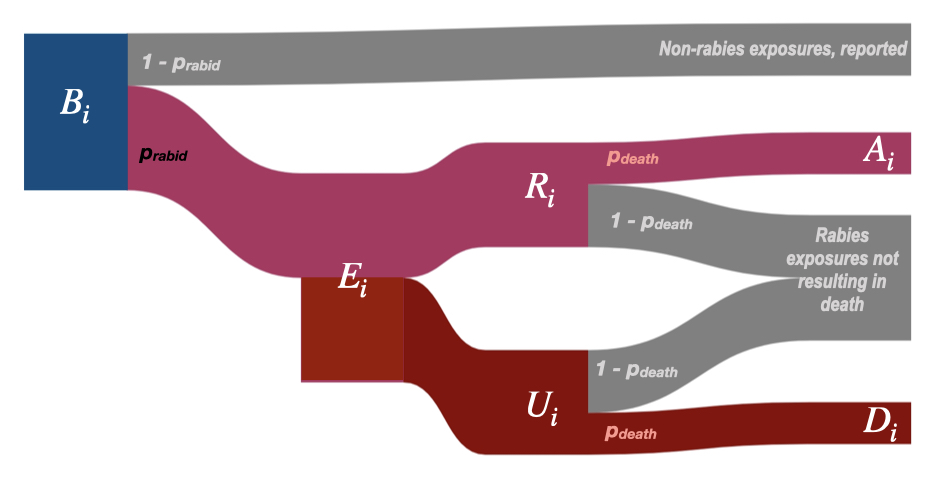
\includegraphics[width=0.9\linewidth]{figs/ch2/fig1} \caption[Decision tree for burden estimation given model predicted bite incidence spatially.]{Decision tree for burden estimation. For a given administrative unit \(i\), human deaths due to rabies (\(D_{i}\)) are calculated from model predicted reported bites
(\(B_{i}\)). To get \(R_{i}\), the number of reported bites that were
rabies exposures, we multiply \(B_{i}\) by \(p_{rabid}\), the proportion
of reported bites that are rabies exposures. \(R_{i}\) is subtracted
from \(E_{i}\) to get the number of unreported bites (\(U_{i}\)) and
then multiplied by the probability of death given a rabies exposure
(\(p_{death}\)) to get deaths due to rabies (\(D_{i}\)). Similarly,
deaths averted by PEP, \(A_{i}\), are estimated by multiplying \(R_{i}\)
by \(p_{death}\), i.e.~those who would have died given exposure, but
instead received PEP. Both \(E_{i}\) and \(p_{rabid}\) are drawn from a
triangular distribution. Parameter values and sources are in Table \ref{tab:ch3-tab1}.}\label{fig:ch3-fig1}
\end{figure}













For \(E_{i}\), we center the distribution at the lower end of our
estimated exposure incidence from the Moramanga District (42
exposures/100,000 persons), with a range applied assuming 1\% rabies
incidence in dogs (estimated across a range of human-to-dog ratios
between 5 - 25) and that on average a rabid dog exposes 0.39 persons
{[}4{]} (see Fig S4.1). As there is little data on dog population size and
human exposure incidence in Madagascar{[}16,23{]}, the range we used
encompasses both observed human-to-dog ratios across Africa {[}14,24{]}
and recent subnational estimates from Madagascar {[}25{]}, and generates
similar exposure incidences as observed previously across Africa
{[}26,27{]}. Given previously high observed compliance in Madagascar
{[}15{]}, we assume that all rabies exposed patients who report to a
clinic receive and complete PEP, and PEP is completely effective at
preventing rabies.

\hypertarget{estimating-the-impact-of-expanding-pep-provisioning}{%
\subsection{Estimating the impact of expanding PEP provisioning}\label{estimating-the-impact-of-expanding-pep-provisioning}}

We developed a framework to rank clinics by how much their PEP provision
improves access for underserved communities, estimating incremental
reductions in burden and increases in vaccine demand. Specifically, we
aggregated our model-predicted estimates of annual bites to the clinic
level. As multiple clinics may serve a single district or commune, we
allocated bites to clinics according to the proportion of the population
in each administrative unit which were closest. For each clinic, we
simulate throughput by randomly assigning patient presentation dates,
and then assume perfect compliance (i.e.~patients report for all doses)
to generate subsequent vaccination dates. We use these dates to estimate
vial usage given routine vial sharing practices in Madagascar {[}15{]},
but assuming adoption of the WHO-recommended abridged intradermal
regimen (2 x 0.1 ml injections on days 0, 3, and 7 {[}28{]}). For both
burden and vial estimates, we take the mean of 1000 simulations as each
clinic is added.

We simulate expansion first to each district (N = 114) and then to each
commune in the country for all communes with a clinic. We select the
primary clinic (primary health facility, usually with capacity to
provision vaccines) in the highest density grid cell of the
administrative unit as candidates for expansion. For the 85 communes
without a primary clinic, we chose the secondary clinic (secondary
health facility, often without formal vaccination capacity) in the
highest density grid cell. 94 communes lacked any health facilities.
Finally, we explore a scenario where all additional primary clinics
(totaling 1733) provision PEP.

We tested three metrics for ranking additional clinics: 1) The
proportion of people living \textgreater3 hours from a existing PEP clinic that
provisions PEP for which travel times were reduced; 2) This proportion
(1), weighted by the magnitude of the change in travel times and 3) The
mean reduction in travel times for people living \textgreater3 hours from an
existing PEP clinic. We simulated expansion of clinics provisioning PEP
to each district using these three metrics and chose the metric which
decreased burden the most compared to simulations (N = 10) where clinics
were added randomly to districts for the full expansion of PEP. For the
full simulation of expanded access, once clinics reduced travel times
for less than 0.01\% of the population (\textless{} 2400 living greater than \(x\)
hrs away, starting with \(x\) = 3 hrs), we reduced the travel time
threshold by 25\%.

\hypertarget{sensitivity-analysis}{%
\subsection{Sensitivity analysis}\label{sensitivity-analysis}}

To test the effect of our model assumptions on estimates of rabies
burden and vial demand, we did a univariate sensitivity analysis of both
parameters from the models of bite incidence and the decision tree (see
Table S6.1 \& S6.2 for parameter ranges used). We also examined how
systematic variation in rabies incidence with human population size
affected burden estimates. Specifically, if human-to-dog ratios are
positively correlated with human populations (i.e.~dog
ownership/populations are higher in more populated, urban areas), we
might expect higher rabies exposure incidence as population size
increases. Alternatively, if human-to-dog ratios inversely correlate
with population size (i.e.~dog ownership is more common in less
populated, rural areas), we might expect exposure incidence to scale
negatively with population size. We use scaling factors to scale
incidence either positively or negatively with observed population sizes
at the district and commune levels, while constraining them to the range
of exposure incidence used in the main analyses (15.6 - 76 exposures per
100,000 persons, Fig S4.2) and simulated baseline burden, as well as
expanded PEP access.

\hypertarget{data-and-analyses-1}{%
\subsection{Data and analyses}\label{data-and-analyses-1}}

All analyses were done in R version 4.0.2 (2020-06-22) {[}29{]} and using
the packages listed in the supplementary references (Supplementary
appendix, section S7). All processed data, code, and outputs are
archived on Zenodo at \url{http://doi.org/10.5281/zenodo.4064312} and
\url{https://doi.org/10.5281/zenodo.4064304}, and maintained at
\url{https://github.com/mrajeev08/MadaAccess}. The raw bite patient data at
the national level are maintained in two secure REDCap
(project-redcap.org) databases, one for IPM and another for all
peripheral clinics provisioning PEP. These databases were last queried
on September 19, 2019 for these analyses. The IPM GIS unit provided the
data on geolocated clinics across the country. Anonymized raw bite
patient data and full data on geolocated clinics are available from IPM
following institutional data transfer protocols. Anonymized raw data
collected from the Moramanga District were retrieved from the Wise
Monkey Portal (wisemonkeyfoundation.org) on the same date and are shared
in the archived repository.

\hypertarget{ethics-statement-1}{%
\subsection{Ethics statement}\label{ethics-statement-1}}

Data collection from the Moramanga District was approved by the
Princeton University IRB (7801) and the Madagascar Ministry of Public
Health Ethics Committee (105-MSANP/CE). Oral informed consent was
obtained from all interviewed participants. Data collected from bite
patients at the national level are maintained jointly by the Ministry of
Health and IPM as a routine part of PEP provisioning.

\hypertarget{results-1}{%
\section{Results}\label{results-1}}

\hypertarget{estimates-of-travel-times-to-clinics-are-high-and-variable-across-madagascar.}{%
\subsection{Estimates of travel times to clinics are high and variable across Madagascar.}\label{estimates-of-travel-times-to-clinics-are-high-and-variable-across-madagascar.}}

Based on the estimates from the friction surface, approximately 36\% of
the population of Madagascar are estimated to live over 3 hours from a
clinic (Fig \ref{fig:ch3-fig2}). However, we found that these estimates underestimated
both driving times across the country and patient-reported travel times
to the Moramanga PEP clinic (Fig \ref{fig:ch3-fig2}C). Patient reported travel times were
highly variable for a given commune compared to the estimated travel
times (Fig S1.2), potentially due to the fact that the friction surface
assumes that the fastest available mode of transport is used across each
grid cell (i.e.~the presence of a road indicates that all travel through
that grid cell is by vehicle). However, patients reported using multiple
modes of transport, with some individuals walking days to the Moramanga
PEP clinic (Fig S1.3).

While the travel time estimates may not reflect exact distributions of
travel times, they were correlated with ground-truthed driving and
patient-reported times and likely reflect patterns of access over the
country (Fig \ref{fig:ch3-fig3}C, Fig S1.4). Travel times weighted by population at the
grid cell level were a better predictor than unweighted travel times or
distance (R\textsuperscript{2} = 0.43, Table S1.1), therefore, we use
population-weighted travel time as a proxy for access at the
commune/district level in subsequent analyses.

\begin{figure}
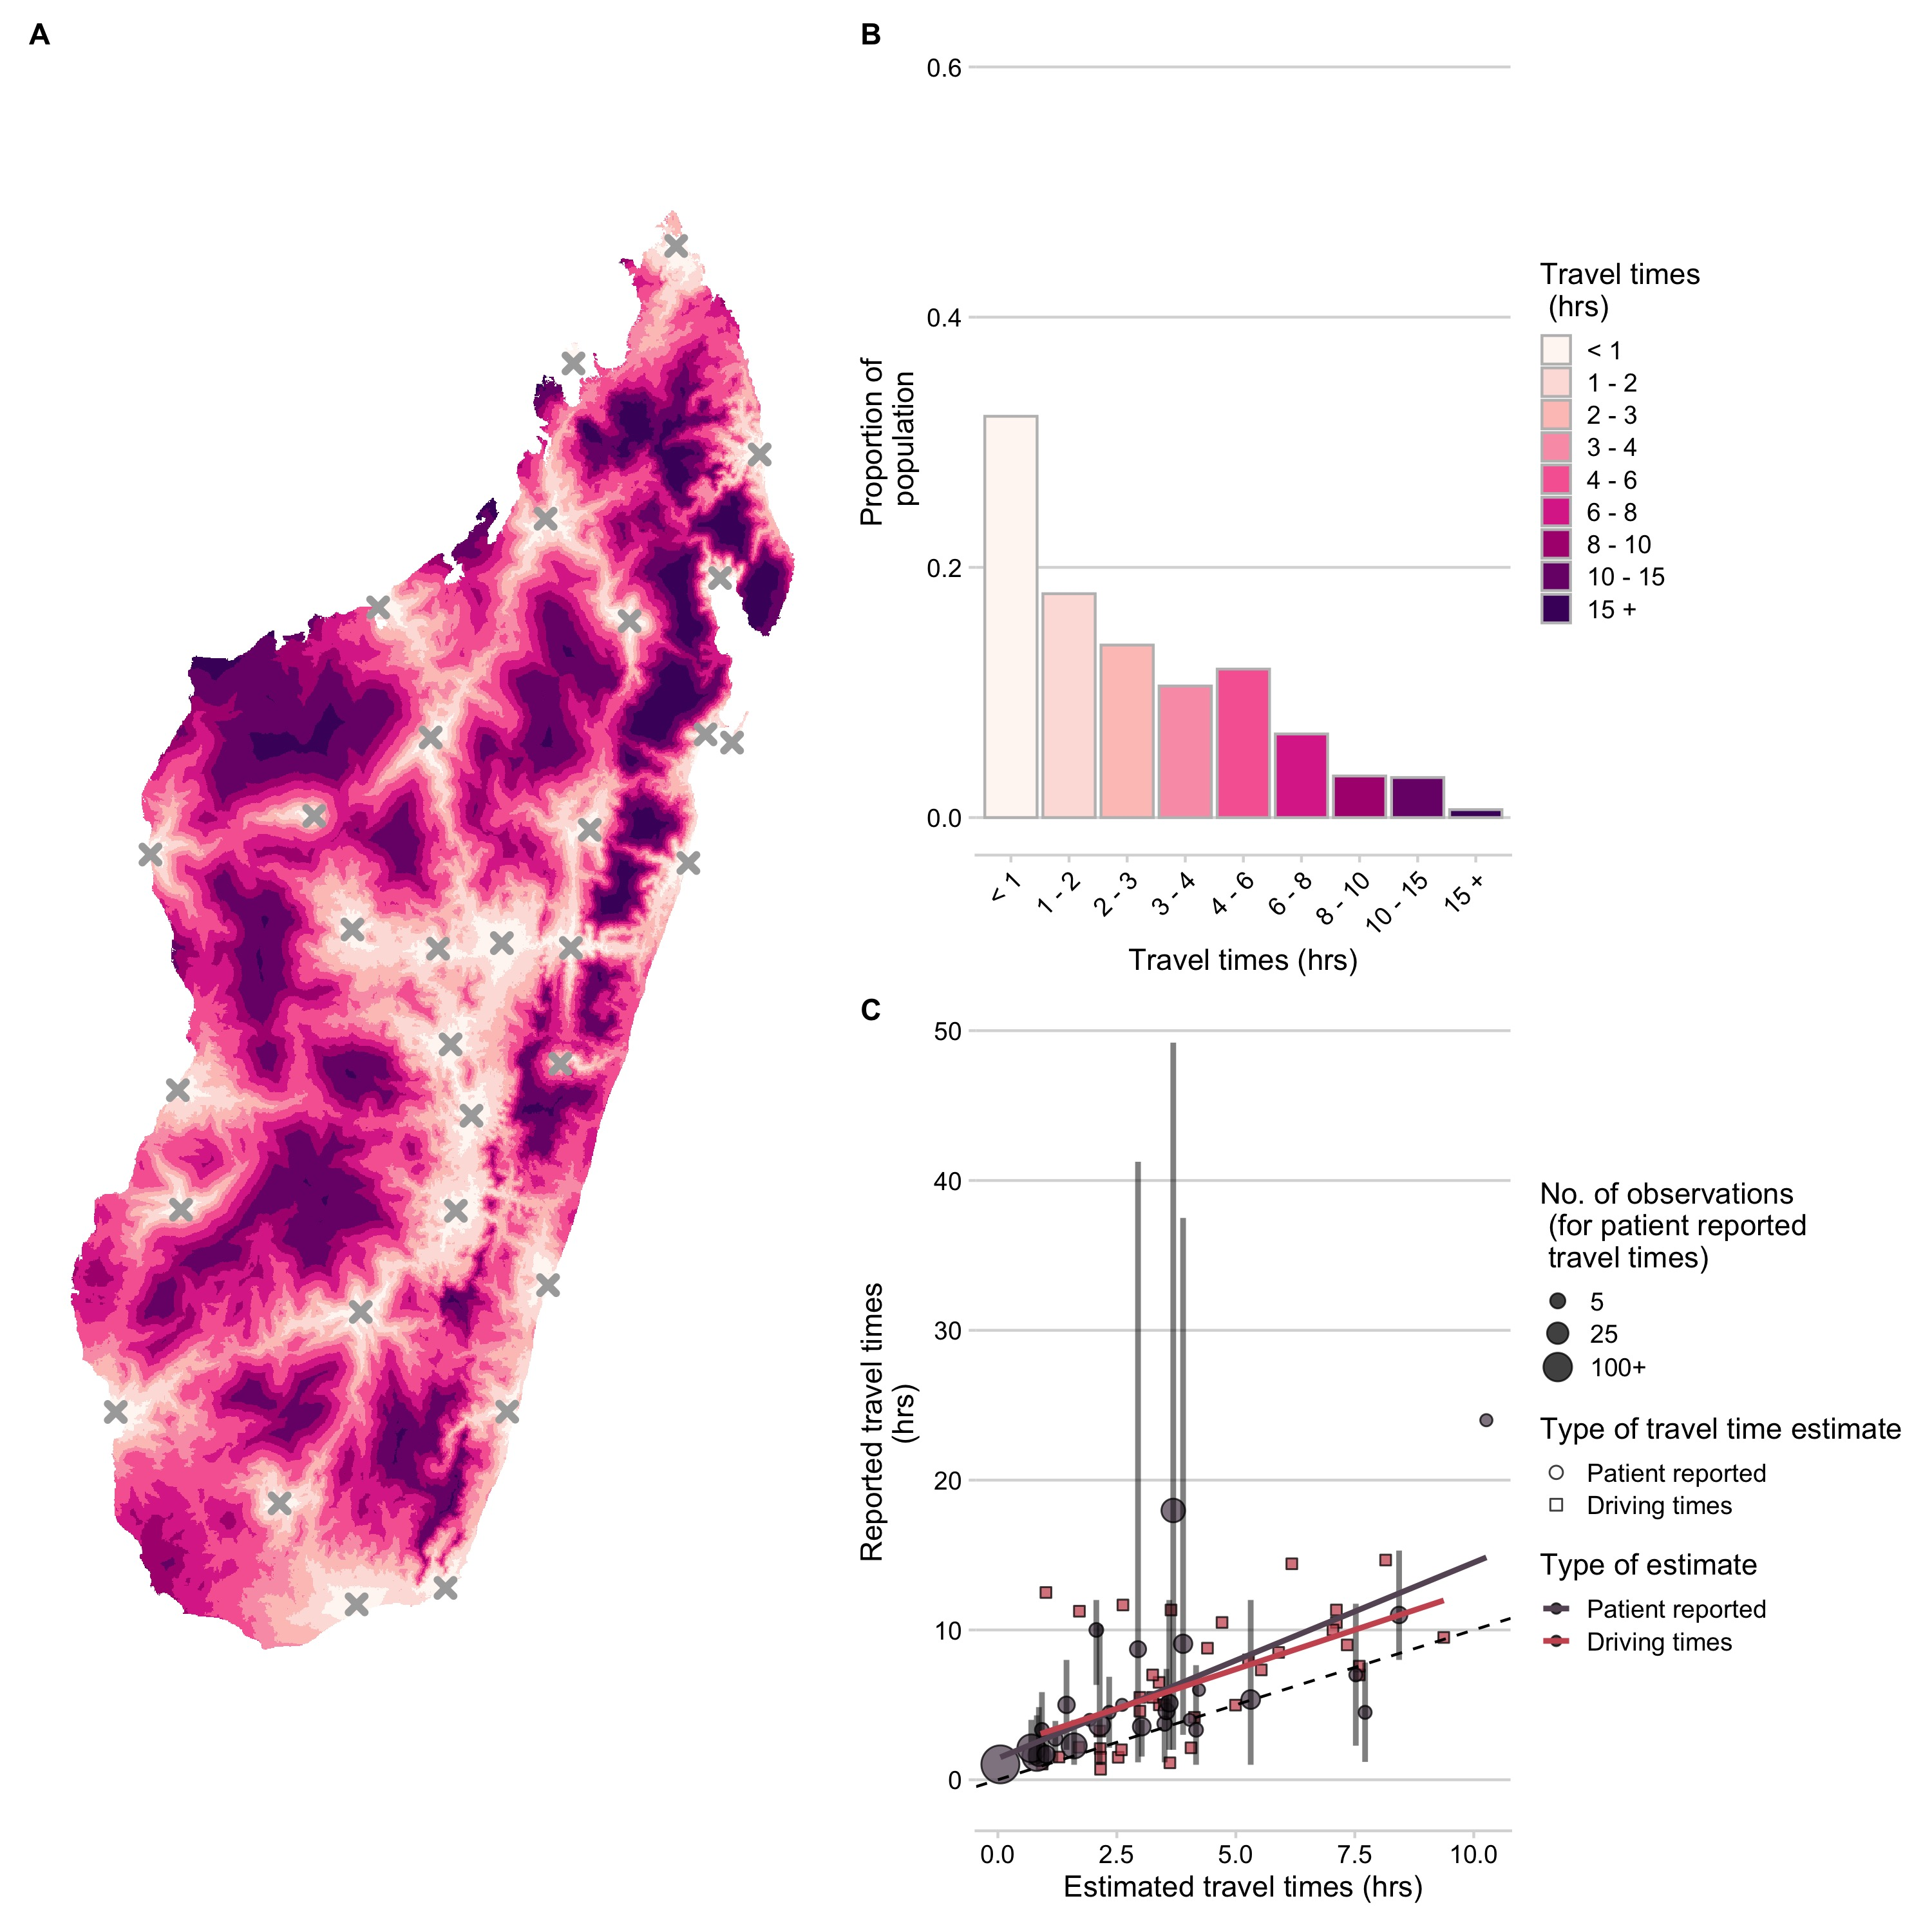
\includegraphics[width=0.9\linewidth]{figs/ch2/fig2} \caption[Travel times to clinics provisioning PEP across Madagascar.]{Travel times to clinics provisioning PEP across Madagascar. (A) Estimated at an \textasciitilde{} 1 km2 scale. (B) Distribution of the population
across travel times. (C) Correlation between ground-truthed travel times
(mean of patient reported travel times to the Moramanga PEP clinic at
the commune level and reported driving times between GPS points) and
friction surface travel time estimates. The vertical lines show the 95\%
quantiles for reported travel times and the point size shows the number
of observations for each commune. The best fit lines (red and grey) from
a linear model where observed travel times are predicted by estimated
travel times for each data source are also shown. The dashed black line
is the 1:1 line.}\label{fig:ch3-fig2}
\end{figure}












\hypertarget{as-travel-times-increase-reported-bite-incidence-decreases.}{%
\subsection{As travel times increase, reported bite incidence decreases.}\label{as-travel-times-increase-reported-bite-incidence-decreases.}}

Bite incidence estimates generally increased with decreasing weighted
travel times at both administrative scales (district and commune),
although there was considerable variation between catchments for the
magnitude of this relationship (Fig \ref{fig:ch3-fig3}C and D). After additionally
excluding any year with less than 25\% of forms submitted, our final
dataset consisted of estimates of average bite incidence for 83 of 114
districts (Fig \ref{fig:ch3-fig3}C), and 58 communes within the catchment of the
Moramanga District (Fig \ref{fig:ch3-fig3}D, see Supplementary Appendix section S2 for
more details). For the national data, there were two outliers, Toamasina
II (the sub-urban district surrounding the city of Toamasina) and
Soanierana Ivongo, with higher bite incidence when compared to other
districts with similar travel times. While the estimates from the
Moramanga data showed higher reported incidence at low travel times at
the commune level compared to the district estimates, when aggregated to
the district, bite incidence estimates fell within the ranges observed
from the national dataset.

\begin{figure}
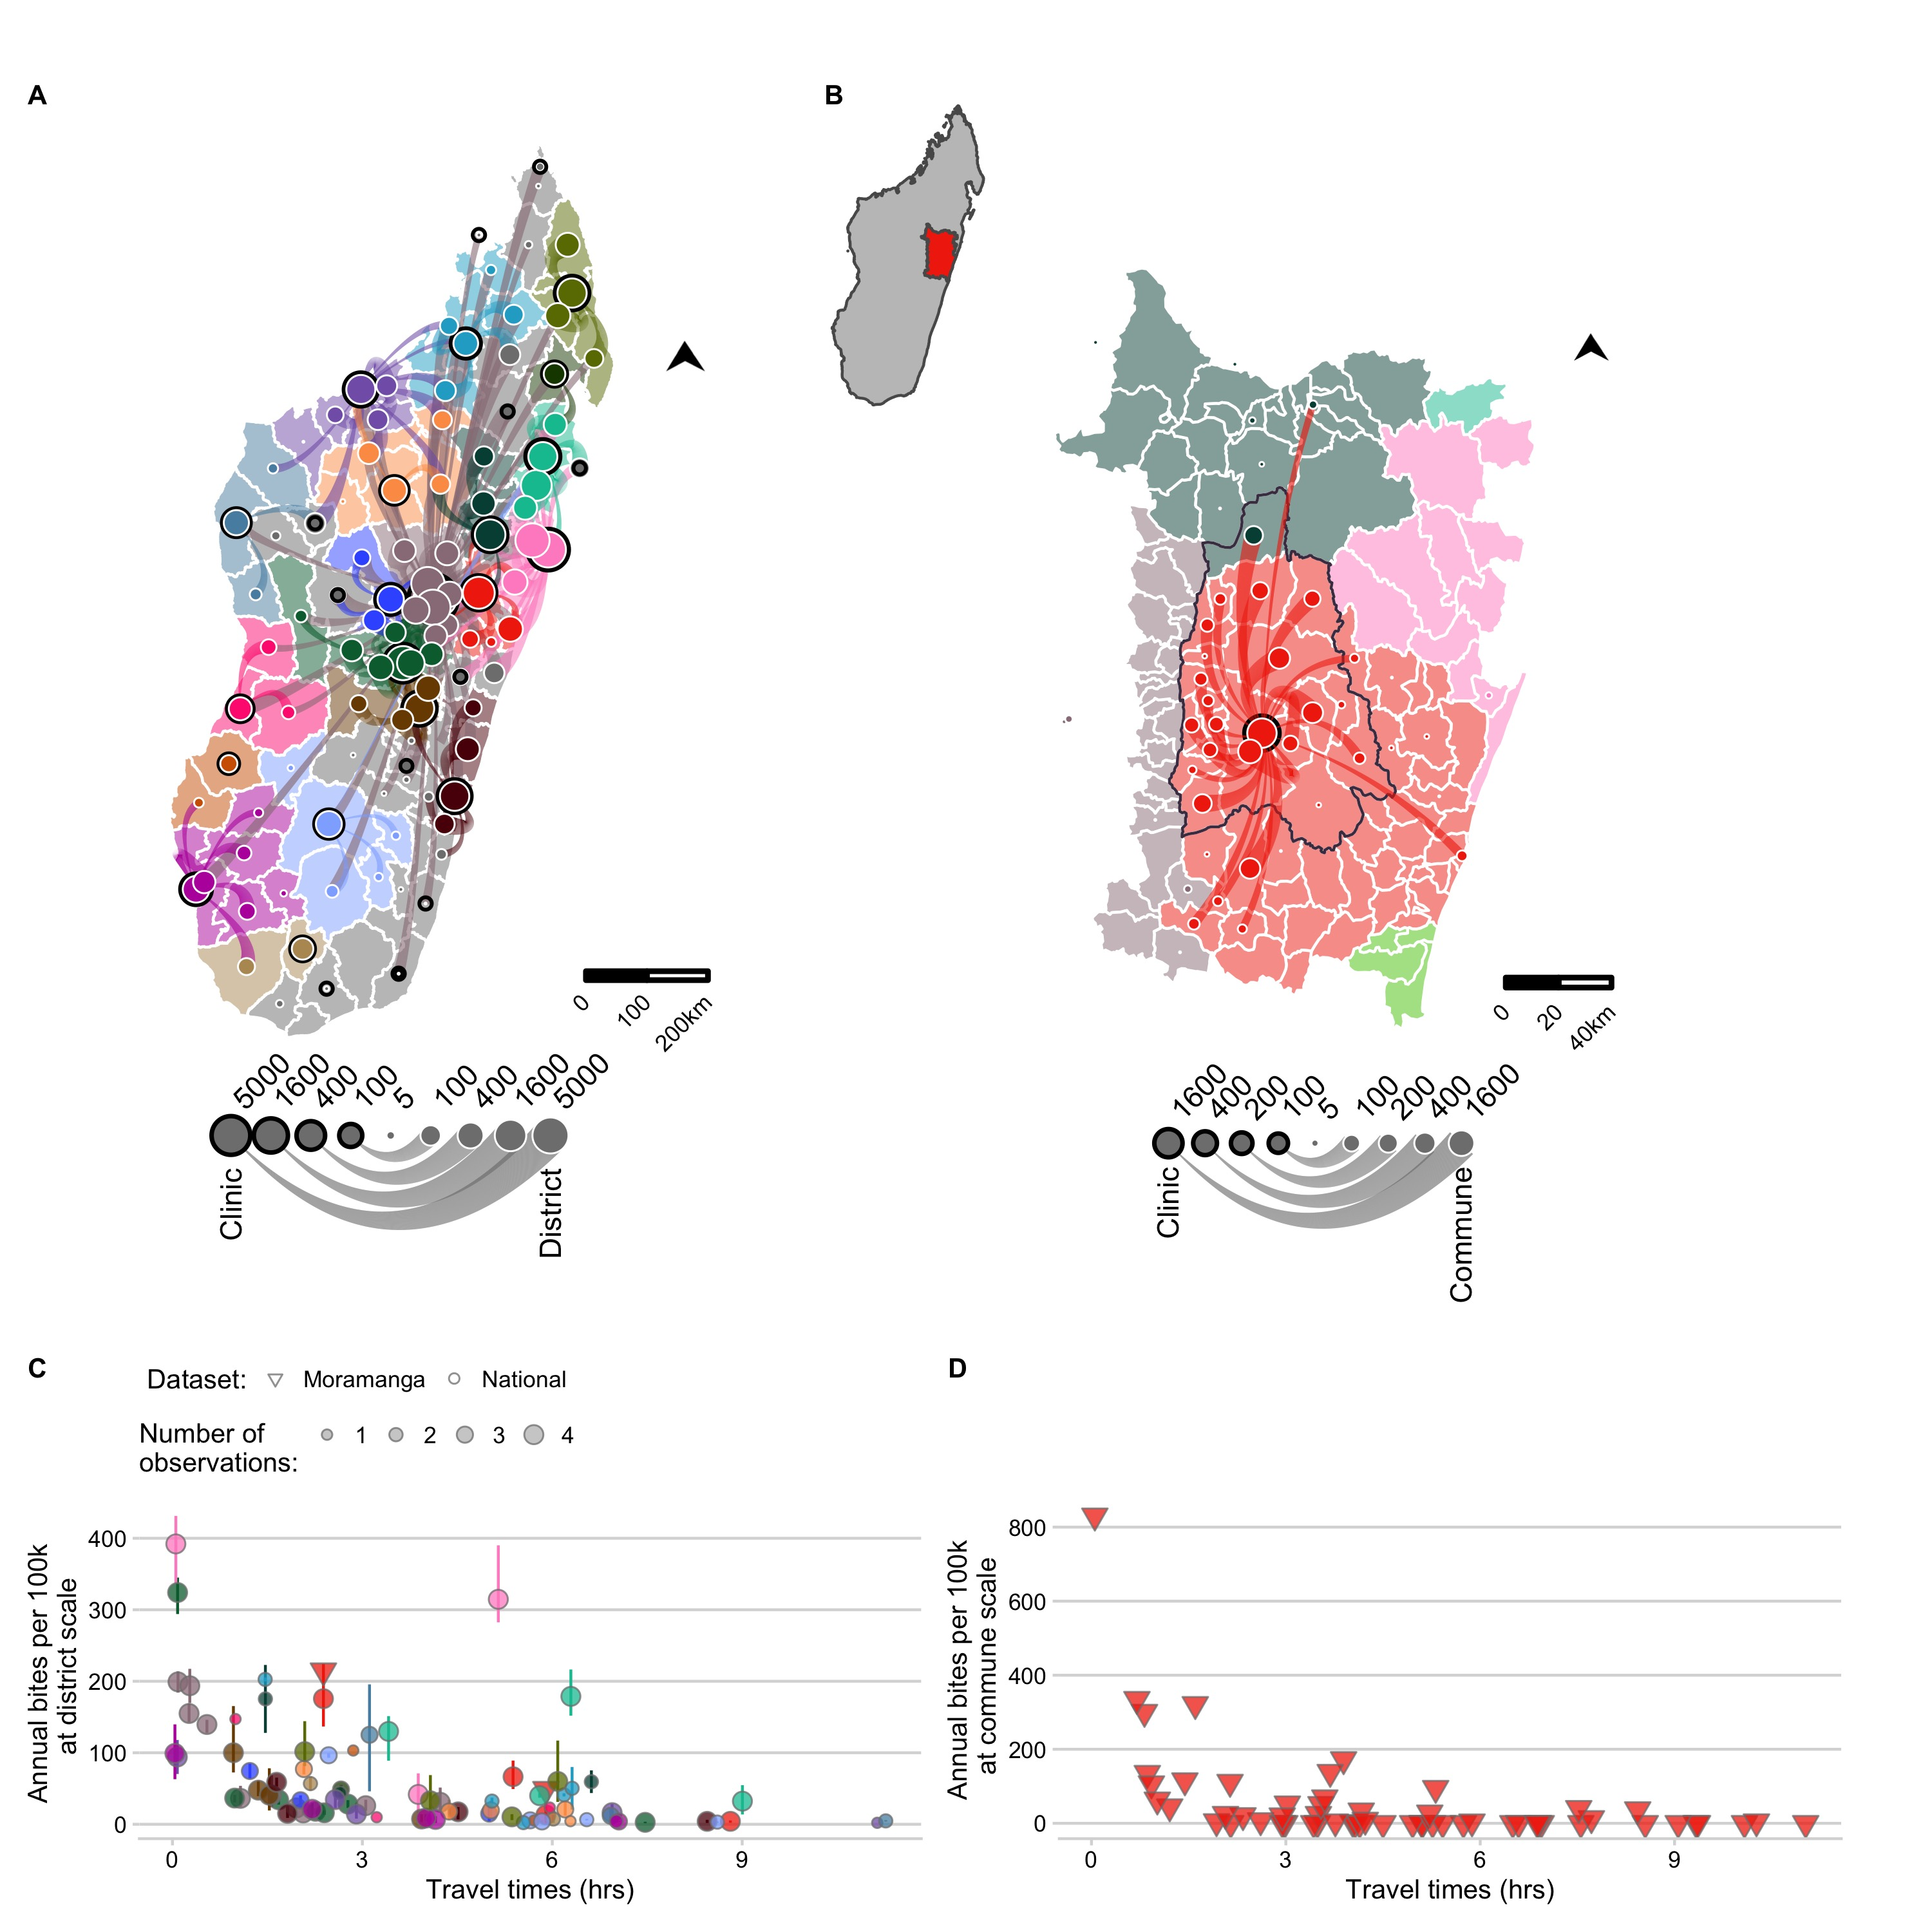
\includegraphics[width=0.9\linewidth]{figs/ch2/fig3} \caption[The network of patient presentations and estimates of annual bite incidence across Madagascar.]{The network of patient presentations and estimates of annual bite incidence. (A) at the district level for the national data and (B) commune level
for the Moramanga data: circles with a black outline represent the total
number of patients reporting to each clinic for which we have data.
Color corresponds to the clinic catchment. Circles with a white outline
are the total number of bites reported for that administrative unit
(plotted as the centroid). Lines show which clinic those patients
reported to, with the line width proportional to number of patients from
that district reporting to the clinic; flows of less than 5 patients
were excluded. Out-of-catchment reporting is indicated where points and
line colors are mismatched. For panel (A) districts in catchments
excluded due to lack of forms submitted by the clinic are colored in
grey. For (B) the inset of Madagascar shows the location of the enlarged
area plotted, which shows the district of Moramanga (outlined in black),
all communes included in it's catchment (red polygons), and other
communes where bites were reported to colored by their catchment (C) The
estimated average annual bite incidence from the national and Moramanga
data plotted at the district scale (both datasets) and at the (D)
commune scale (Moramanga dataset). Colors correspond to the clinic
catchment, shape indicates the dataset, and the size of the point
indicates the number of observations (i.e.~the number of years for which
data was available for the national data; note for Moramanga 33 months
of data were used). The point lines indicate the range of estimated bite
incidence for each district.}\label{fig:ch3-fig3}
\end{figure}

























Our modeling results show that travel times were a strong and consistent
predictor of reported bite incidence in both datasets and across scales
with the best fitting models including travel times and an
overdispersion parameter (Fig \ref{fig:ch3-fig4}, see Supplementary Appendix section S3
for comparisons to models with catchment effects and with population
size as a covariate). As the predictions of the model fit to the
Moramanga data without accounting for overdispersion fall within the
prediction intervals for the models fit to the national data (Fig \ref{fig:ch3-fig4}A),
for subsequent predictions, we used the parameter estimates from models
fit to the national data, which encompass the range of travel time
effects observed in our datasets. Moreover, our out-of-fit predictions
to the data across scales suggest that the commune model is able to
capture travel time impacts at the commune level (Fig S3.3), therefore
we use both the district and commune model to disaggregate burden to the
finest scale possible. Finally, we examined the sensitivity of models to
how we corrected for underreporting of data and found that parameter
estimates of travel time impacts were similar across models and
performed similarly in prediction (Fig S3.8 and Fig S3.9).

\begin{figure}
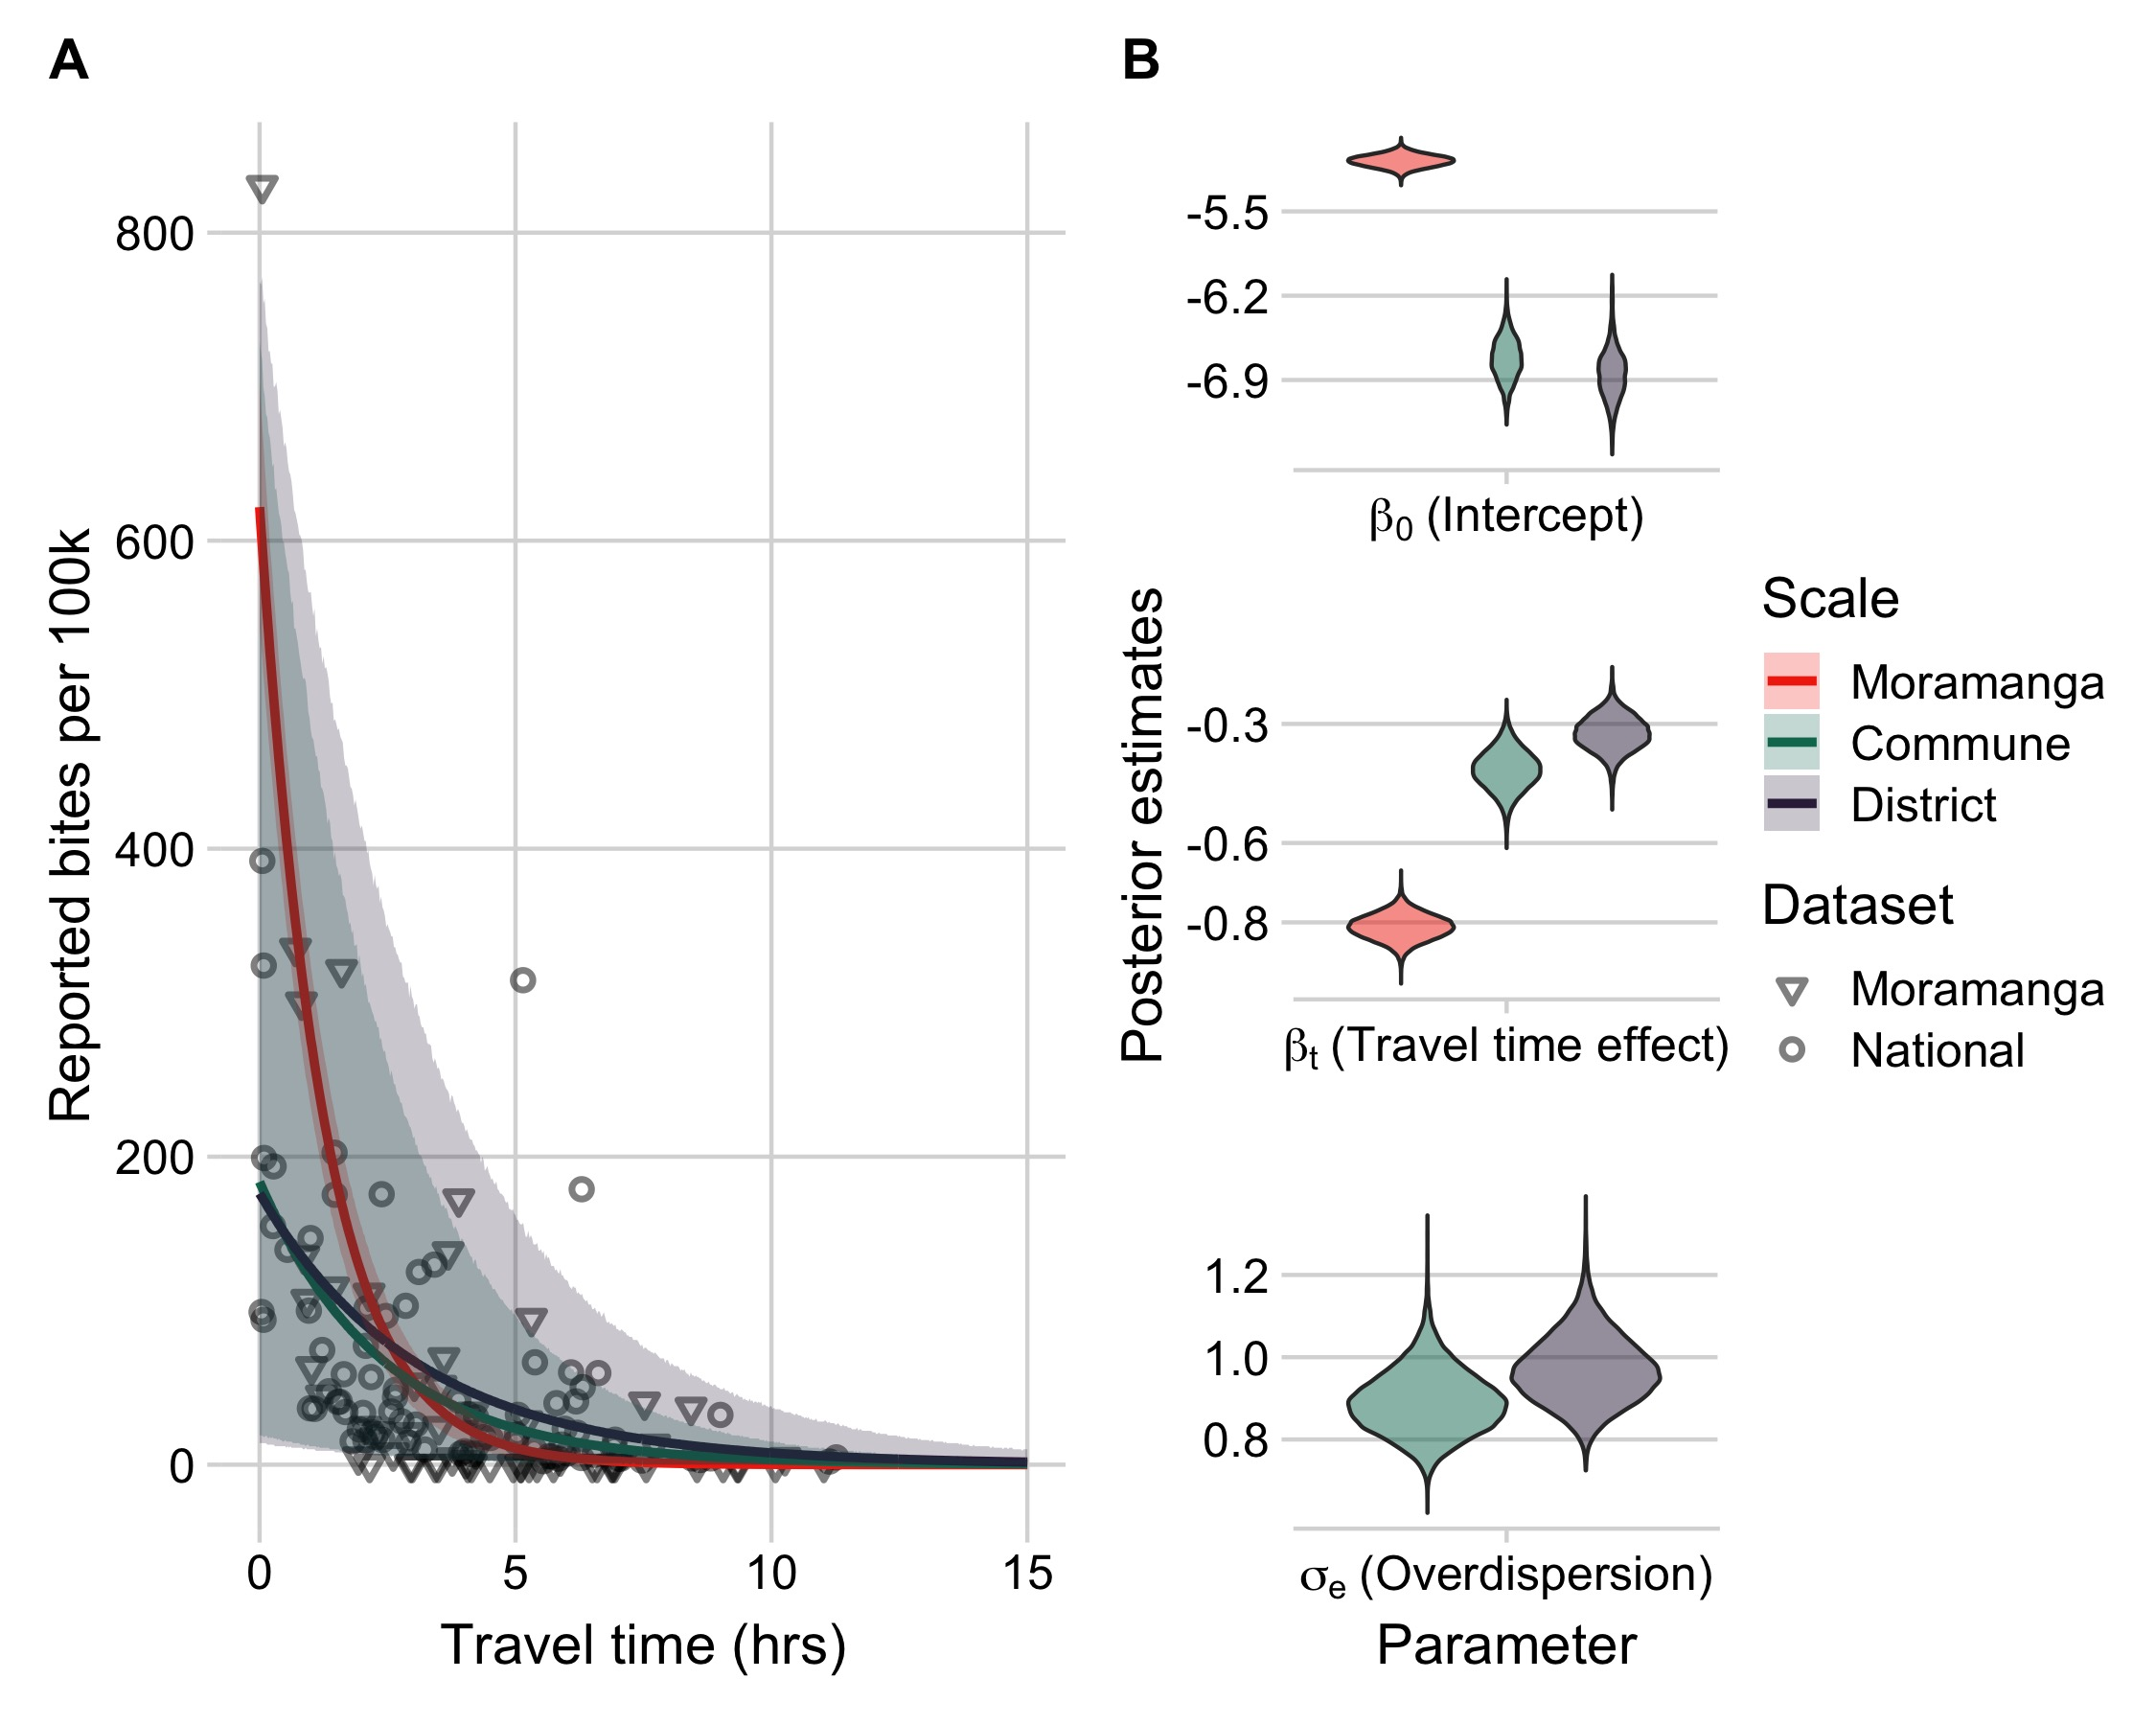
\includegraphics[width=0.9\linewidth]{figs/ch2/fig4} \caption[Travel times as a predictor of reported bite incidence per 100,000 persons.]{Travel times as a predictor of reported bite incidence per 100,000 persons. (A) The estimated relationship between travel time in hours (x-axis)
and mean annual reported bite incidence (y-axis). The lines are the mean
estimates and the envelopes are the 95\% prediction intervals generated
by drawing 1000 independent samples from the parameter posterior
distributions for three candidate models: model with travel times at the
1) commune- and 2) district-level fitted to the national data with an
overdispersion parameter (\(\sigma_{e}\)) and 3) travel times at the
commune level fitted to the Moramanga data with a fixed intercept and
unadjusted for overdispersion. The points show the data: National data
(circles) at the district level used to fit the District and Commune
models, and Moramanga data (triangles) at the commune level used to fit
the Moramanga model. (B) The posterior distribution of parameters from
the respective models for the model intercept, travel time effect, and
for overdispersion (national data only).}\label{fig:ch3-fig4}
\end{figure}
















\hypertarget{current-provisioning-of-pep-substantially-reduces-human-rabies-deaths-but-incidence-of-deaths-remains-high-in-areas-with-poor-access}{%
\subsection{Current provisioning of PEP substantially reduces human rabies deaths, but incidence of deaths remains high in areas with poor access}\label{current-provisioning-of-pep-substantially-reduces-human-rabies-deaths-but-incidence-of-deaths-remains-high-in-areas-with-poor-access}}

In general, the incidence of rabies deaths increases with travel times
to clinics, and there is significant sub-national variation when deaths
are modeled at the district and commune scale, with the least accessible
communities having most deaths (Fig \ref{fig:ch3-fig5}B \& C). We estimate that under the
current system of 31 clinics in Madagascar provisioning PEP that
approximately 800 (95\% PI: 600 - 1000) deaths due to rabies are
prevented through PEP each year. Overall, we estimate close to 1000
rabies deaths (95\% PI: 800 - 1100) annually in Madagascar. Our estimates
vary only slightly depending on the scale of the model (Table \ref{tab:ch3-tab2}), but
disaggregating deaths to the commune level shows considerable variation
in predicted burden within districts (Fig \ref{fig:ch3-fig5}A).

\begin{longtable}[]{@{}
  >{\raggedright\arraybackslash}p{(\columnwidth - 6\tabcolsep) * \real{0.09}}
  >{\raggedright\arraybackslash}p{(\columnwidth - 6\tabcolsep) * \real{0.32}}
  >{\raggedright\arraybackslash}p{(\columnwidth - 6\tabcolsep) * \real{0.17}}
  >{\raggedright\arraybackslash}p{(\columnwidth - 6\tabcolsep) * \real{0.42}}@{}}
\caption{\label{tab:ch3-tab2} Model predictions of average annual reported bite incidence, total deaths, and deaths averted at the national level for the two models (commune level and district level models with travel time predictor and an overdispersion parameter); 95\% prediction interval in parentheses.}\tabularnewline
\toprule
Model & Reported bite incidence per 100k & Burden of deaths & Deaths averted by current PEP provisioning \\ \addlinespace
\midrule
\endfirsthead
\toprule
Model & Reported bite incidence per 100k & Burden of deaths & Deaths averted by current PEP provisioning \\ \addlinespace
\midrule
\endhead
Commune & 85 (56 - 129) & 963 (795 - 1118) & 801 (644 - 968) \\ \addlinespace
District & 85 (52 - 136) & 958 (752 - 1156) & 807 (609 - 1005) \\ \addlinespace
\bottomrule
\end{longtable}

\begin{figure}
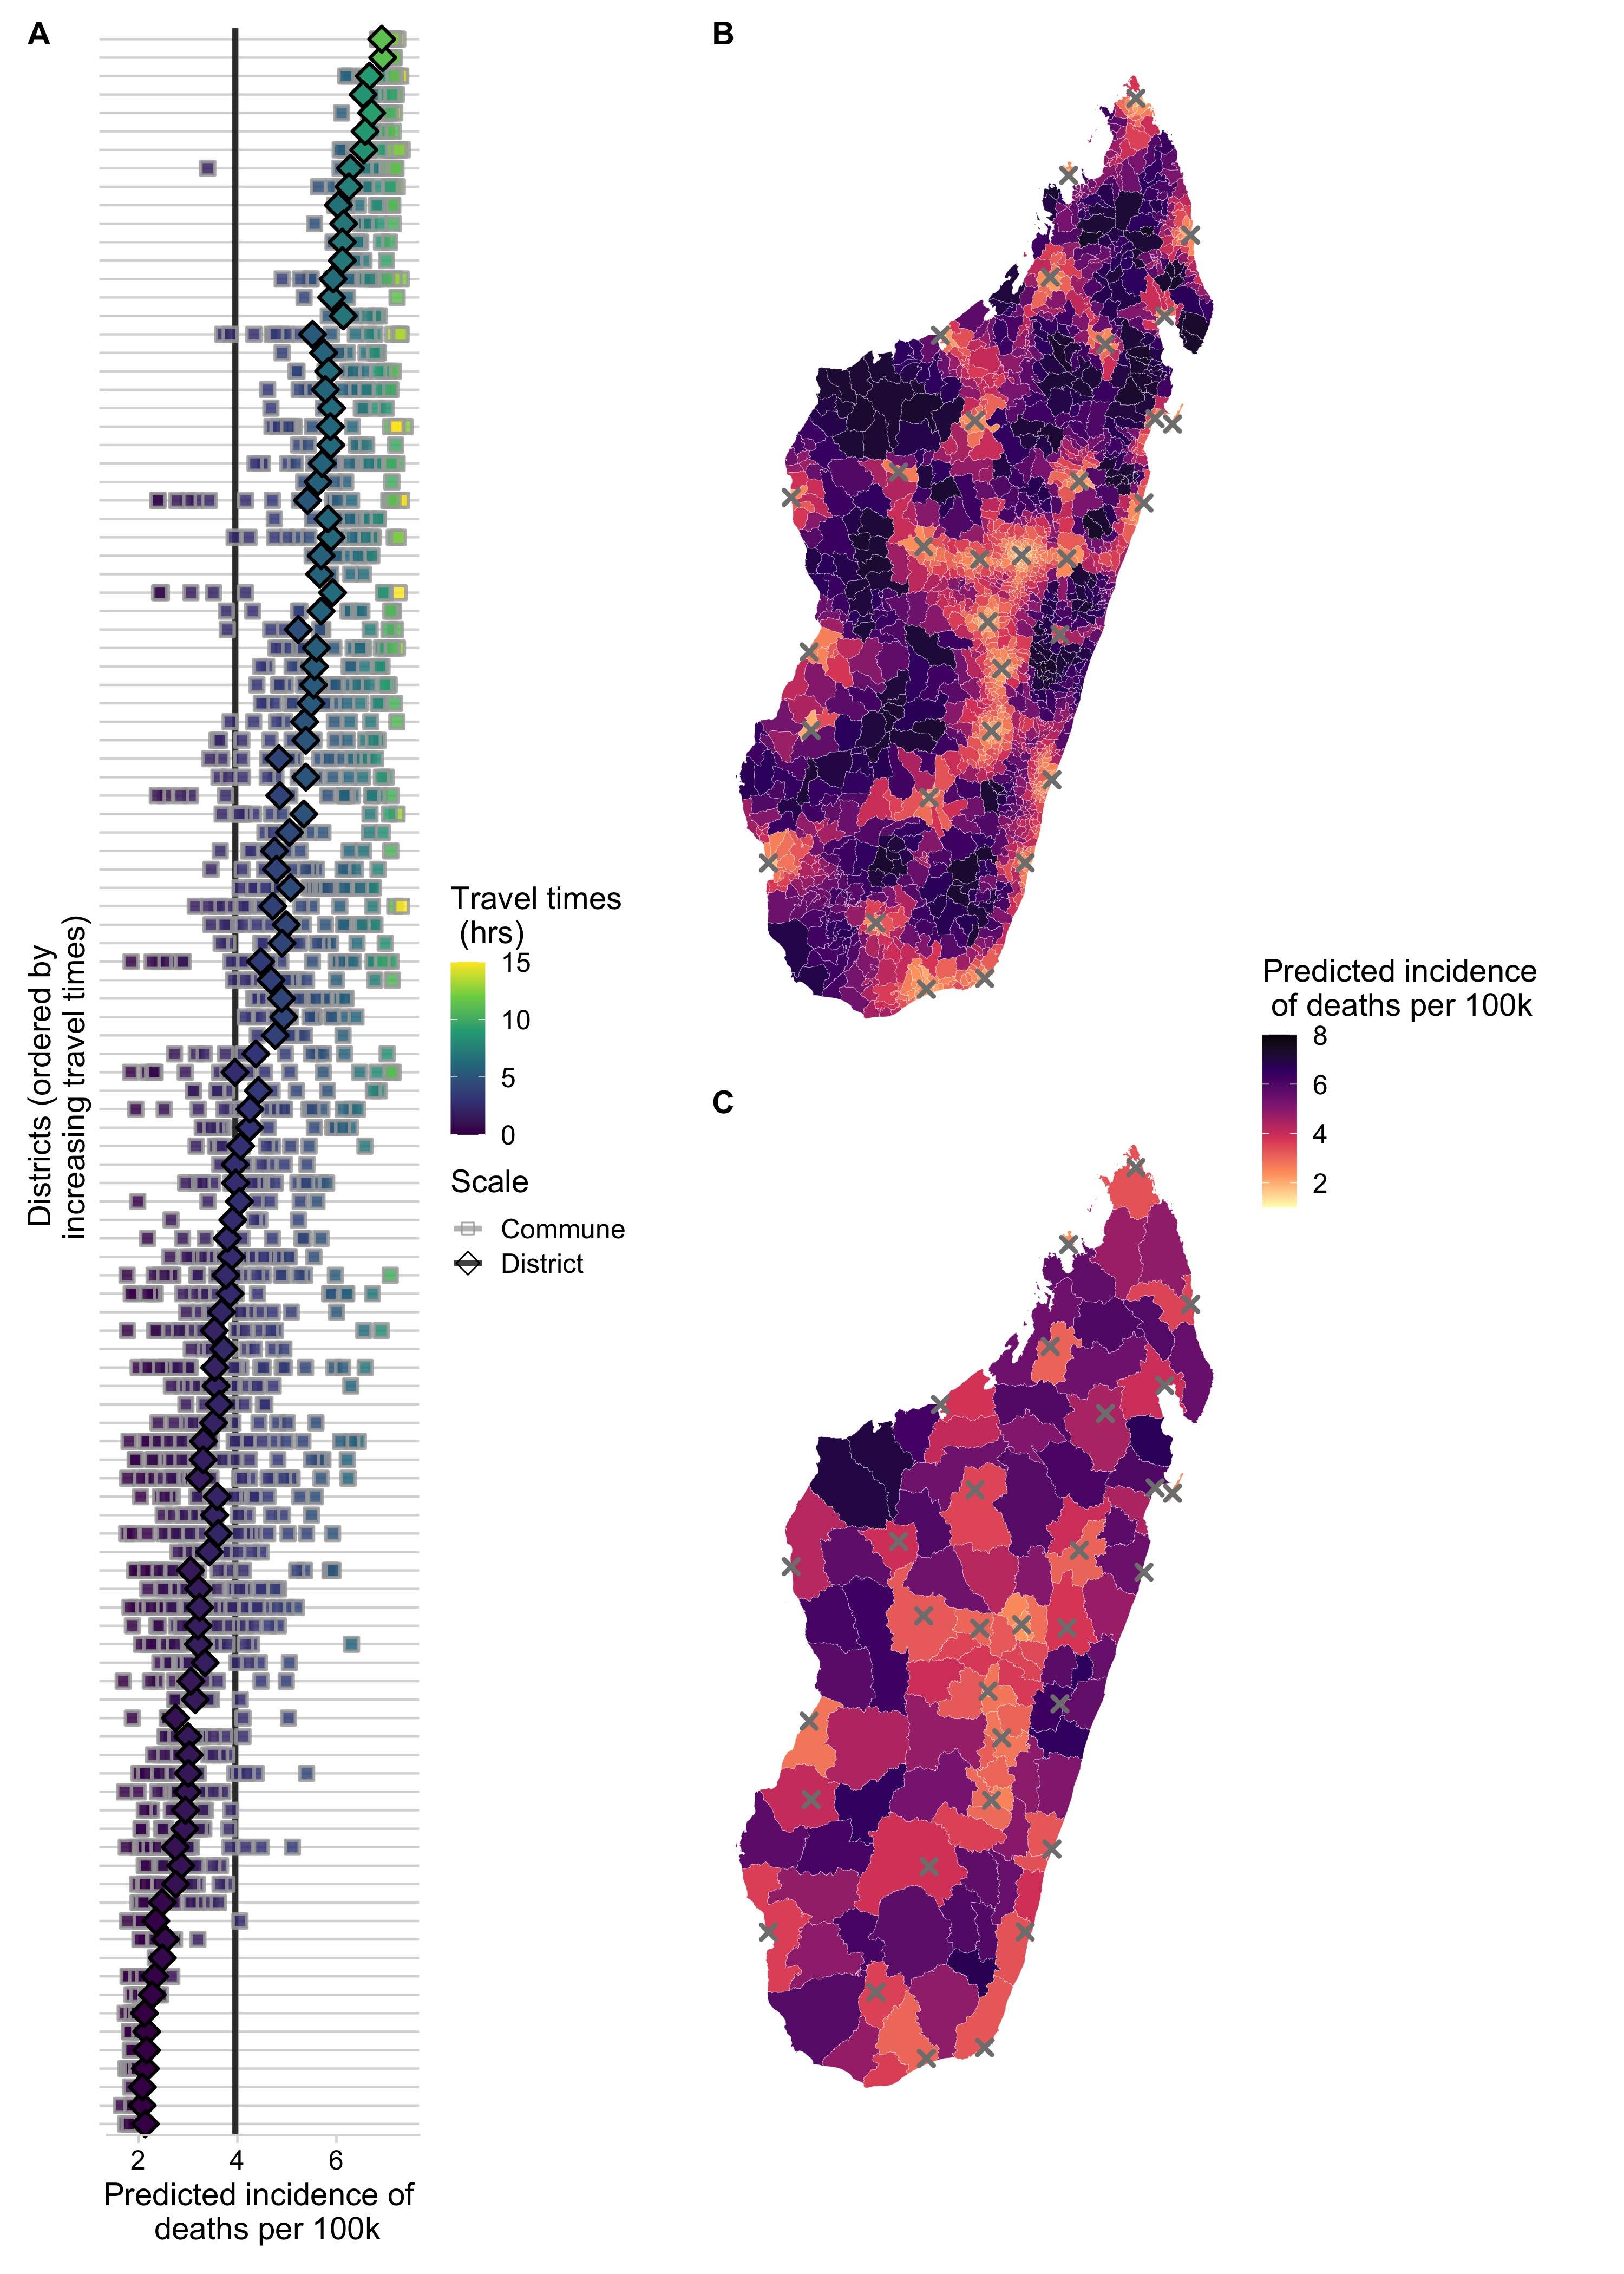
\includegraphics[width=0.9\linewidth]{figs/ch2/fig5} \caption[Spatial variation in predicted incidence of human rabies deaths per 100,000 persons.]{Spatial variation in predicted incidence of human rabies deaths per 100,000 persons. (A) for each district (y-axis) in Madagascar. Diamonds show the
predicted incidence for the district model and squares show predicted
incidence for the commune model fit to the National data for all
communes in a district. Points are colored and districts ordered by
travel times. The vertical lines show the average national incidence of
human rabies deaths for the commune (grey) and district (black) models.
Incidence mapped to the (B) commune- and (C) district-level from the
respective models; grey X's show locations of current clinics
provisioning PEP.}\label{fig:ch3-fig5}
\end{figure}











\hypertarget{expanding-pep-access-to-underserved-populations-is-effective-at-reducing-human-rabies-deaths-but-this-effect-saturates-as-more-clinics-provision-pep}{%
\subsection{Expanding PEP access to underserved populations is effective at reducing human rabies deaths, but this effect saturates as more clinics provision PEP}\label{expanding-pep-access-to-underserved-populations-is-effective-at-reducing-human-rabies-deaths-but-this-effect-saturates-as-more-clinics-provision-pep}}

We found that targeted expansion of PEP to clinics based on the
proportion of the population they reduced travel times for resulted in
fewest deaths (Fig S5.1). Here we report results from the commune model,
as estimates were consistent across models (Fig \ref{fig:ch3-fig6} and Supplementary
appendix, section S5). We estimated that strategic PEP expansion to
these additional 83 clinics (1 per district) reduced rabies deaths by
19\% (95\% PI: 14 - 23\%) (Fig \ref{fig:ch3-fig6}A). With one clinic per commune (where
available, N = 1696), we see a further reduction of 38\% (95\% PI: 30 -
46\%). However, reductions in burden saturate as more clinics are added
(Fig S5.2). Even when all primary clinics provision PEP, our model still
predicts 600 (95\% PI: 400 - 800) deaths per annum, and average reporting
of rabies exposures remains approximately 66\% (95\% PI: 33 - 78\%) (Fig
S5.5); as more clinics are added, reported bite incidence saturates (Fig
S5.4), and patients shift which clinic they report to (S5.7 \& S5.8).

Vial demand also outpaces reductions in burden (Fig \ref{fig:ch3-fig6}B), with more vials
needed per death averted (Fig \ref{fig:ch3-fig6}C). Our model predicts an increase from
33500 vials (95\% PI: 22900 - 49400) per annum under current provisioning
but with the abridged intradermal regimen (i.e.~visits on days 0, 3, 7),
to \textasciitilde56900 vials (95\% PI: 40200 - 77800) with 250 clinics providing PEP,
and \textasciitilde86400 vials (95\% PI: 61600 - 118000) if all primary clinics
provision PEP. In these scenarios, clinic catchment populations and
throughput decrease, with clinics seeing fewer patients per day (S5.6).

\begin{figure}
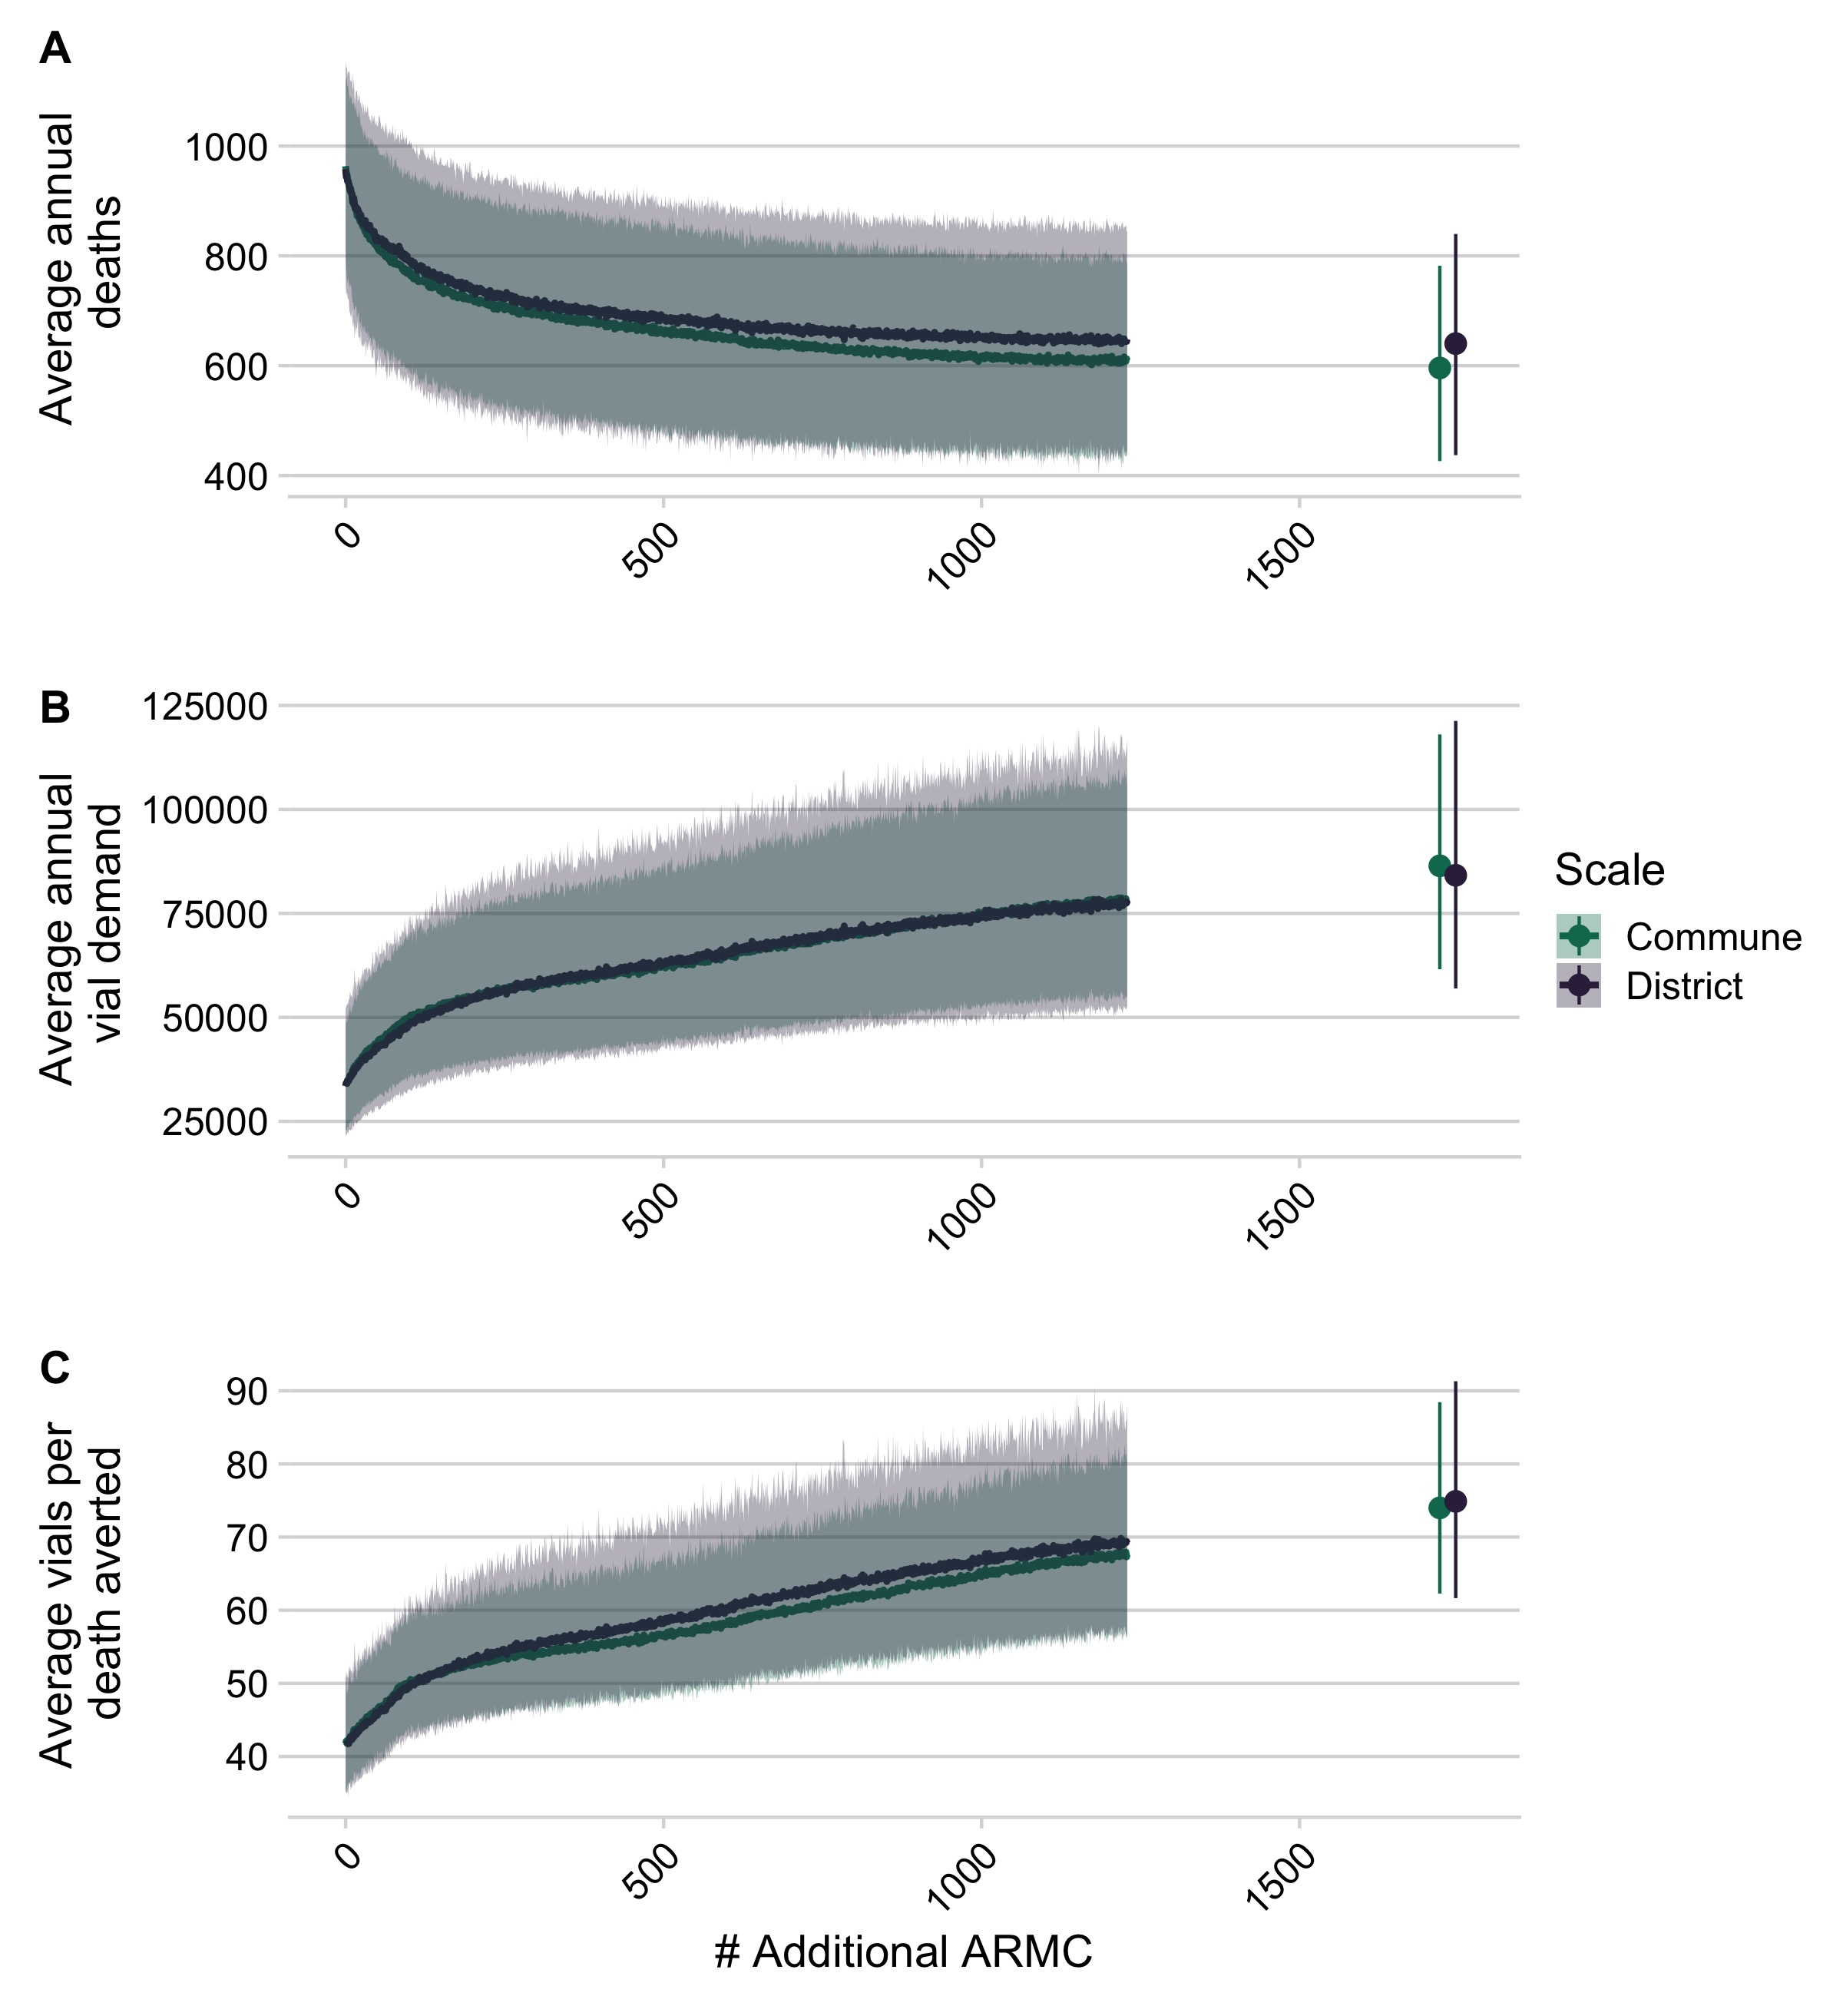
\includegraphics[width=0.9\linewidth]{figs/ch2/fig6} \caption[Impact of expanded PEP access on deaths, deaths averted, and vial demand.]{Impact of expanded PEP access on deaths, deaths averted, and vial demand. (A) Decrease in deaths due to rabies, (B) increase in total \# of vials
as additional clinics provisioning PEP are added at the national level,
and (C) increase in vials needed per death averted based on the two
models of reported bites. Lines are the mean of 1000 simulations with
envelopes representing 95\% prediction intervals. The points show when
all additional primary clinics and secondary clinics (N = 1733) clinics
have been added).}\label{fig:ch3-fig6}
\end{figure}









\hypertarget{burden-estimates-are-most-sensitive-to-assumptions-of-underlying-rabies-incidence.}{%
\subsection{Burden estimates are most sensitive to assumptions of underlying rabies incidence.}\label{burden-estimates-are-most-sensitive-to-assumptions-of-underlying-rabies-incidence.}}

While qualitative patterns of the current impact of geographic access on
human rabies deaths and the impact of expanding access to PEP on
reducing these deaths is robust across a wide range of parameter
estimates, our sensitivity analyses show that assumptions of the
underlying rabies exposure incidence (\(E_{i}\)) contribute the most
uncertainty to our quantitative estimates (Fig S6.1 \& 2). Uncertainty in
bite model parameters contribute less to uncertainty in estimates of
burden or impacts of expanded access. For the estimates of vial demand,
uncertainty around the model intercept (i.e.~the baseline reported bite
incidence) has most impact, rather than the travel time effect or the
overdispersion parameter (Fig S6.3). Finally, scaling of incidence with
population size (Fig S4.2) modulates the impact of travel times on
deaths, with positive scaling of rabies incidence with population size
(i.e.~more rabies in more populated places) dampening and negative
scaling exacerbating the relationship between access and deaths (Fig
S6.4A). However, the impact of adding clinics remains broadly the same
(Fig S6.4B).

\hypertarget{discussion-1}{%
\section{Discussion}\label{discussion-1}}

\hypertarget{main-findings}{%
\subsection{Main findings}\label{main-findings}}

We find that the burden of rabies in Madagascar is likely concentrated
in areas with poor PEP access. We estimate that current PEP provisioning
(at 31 clinics) averts 45\%of deaths that would otherwise occur, and that
expanding PEP access should reduce mortality, with provisioning in one
clinic per district (N = 83), or per commune (N = 1733), expected to
reduce mortality by 16\% and 33\%, respectively. However, improved PEP
provisioning is unlikely to eliminate rabies deaths; with over 600
deaths expected even with PEP at all primary clinics (N = 1733). This is
partly because travel times remain high (\textgreater{} 2 hrs as estimated by the
friction surface for over 10\% of the population, Fig S5.4) even after
expanding PEP to all primary clinics. With reduced travel times, over
20\% of exposures will still not seek PEP (Fig S5.5), resulting in \textasciitilde1.65
rabies deaths per 100,000 people. PEP is expected to remain
cost-effective as provisioning expands, to a maximum of 450 USD per
death averted (assuming 5 USD per vial), similar to other estimates
{[}4{]}. While our quantitative predictions depend on assumptions of
underlying rabies exposure incidence, the qualitative patterns regarding
travel time impacts remain robust and are useful in identifying
strategies for provisioning PEP.

\hypertarget{limitations}{%
\subsection{Limitations}\label{limitations}}

Data limitations introduced bias and uncertainty to our estimates. For
example, travel times from the Malaria Atlas Project friction surface
underestimated patient-reported travel times, with discrepancies between
assigned transport speeds (from the Open Street Map user community, or
country cluster data {[}18{]}) and realities of local travel. In
Madagascar, the presence of paved roads does not necessarily reflect
their quality or the modes of transport used. Patients seeking PEP at
the Moramanga clinic reported various transport methods and highly
variable travel times even within a single commune. While
patient-reported travel times may lack precision from recall and
estimation error, they likely better reflect lived experience; validated
travel times {[}30{]} could improve estimates of spatial health
inequities. Similarly, modeled estimates of population distribution
{[}19{]} also introduce uncertainty. Our analysis of data from the
Moramanga District indicates that variation at the sub-district level is
high and impacts health seeking behavior. However, we lacked fine-scale
data from other catchments for comparison. Additionally, we had to
correct for underreporting and incomplete data; strengthening
surveillance and routine data collection should improve understanding of
health seeking behavior and access, and support monitoring and
evaluation of PEP provisioning.

While we rely on a number of assumptions, they are based on data
specific to Madagascar or from other similar settings and consistent
with estimates from the literature more broadly (see Table \ref{tab:ch3-tab1} and section
S4). Our burden estimates were most sensitive to assumptions about
rabies exposure incidence, drawn from studies in the Moramanga District
{[}15{]} and elsewhere {[}4{]}. As incidence of rabies exposures varies over
time and space {[}31,32{]}, we incorporated uncertainty into our
estimates, but we did not find qualitative differences in the effects of
travel times on rabies deaths. Our simplifying assumptions regarding
patient compliance, which is generally high in Madagascar {[}15{]}, and on
complete efficacy of PEP are unlikely to greatly influence our burden
estimates {[}22{]}. Likewise, we do not account for differential risk for
severely exposed patients not receiving Immunoglobulins (RIG), which is
only available at IPM in the captial of Antananarivo, but recent studies
show that even in the absence of RIG, PEP is extremely effective {[}4{]}.
We also assume that clinics reliably provision PEP, but a 2019 KAP
survey reported clinics experiencing stock-outs {[}25{]}.

We assumed geographic access to PEP was the primary driver of
health-seeking behavior, but socioeconomic status, education and
awareness about rabies {[}{[}33{]}; {[}27{]}; {[}34{]}; {[}35{]};
castillo2020behavioral{]} all play a role. For example, most PEP clinics
also charge fees (from 0.50 - 3.00 USD for consultations, wound
treatment, etc. {[}25{]}) which may also act as barriers to PEP access. In
Madagascar, where PEP is free-of-charge, the main cost to patients is
transport and time lost. More remote communities tend to be of lower
socioeconomic and educational status {[}2{]}, so travel time may be a
proxy for these correlated variables. Significant overdispersion in the
data that cannot be explained by travel times suggests that clinic-level
variation (e.g.~vaccine availability and charges) and regional
differences (e.g.~dog populations, outbreaks, awareness) further
influence health-seeking behavior and vaccine demand. Although our
estimates could be improved with better data on rabies incidence,
health-seeking behavior, and PEP provisioning, predicting PEP impacts
will remain challenging given the complex interactions between
socioeconomic factors, access to and quality of care, and human
behavior, as illustrated by the case studies in Box 1. However, it is
very likely that the impacts of improving access to PEP could be further
increased with outreach and awareness raising efforts that we were
unable to parameterize.

\hypertarget{box-2-case-studies-of-of-health-seeking-behavior-for-pep-in-madagascar}{%
\subsubsection{Box 2: case studies of of health seeking behavior for PEP in Madagascar}\label{box-2-case-studies-of-of-health-seeking-behavior-for-pep-in-madagascar}}

\begin{enumerate}
\def\labelenumi{\arabic{enumi}.}
\item
  Anosibe An'ala District (population \textasciitilde{} 100,265), south of Moramanga,
  has moderate incidence of bite patients (\textasciitilde{} 54/100,000 persons) even
  though travel times often exceed 24 hours. While a road connects the
  main Anosibe An'ala commune to the Moramanga PEP clinic, it is only
  passable by large trucks during much of the rainy season, with
  speeds usually \textless{} 10km per hour. Over 9\% of patients from Anosibe
  An'ala had been in close proximity or touched a person that died
  from rabies (four suspect human rabies deaths of patients who did
  not receive any PEP), whilst of patients with Category II and III
  exposures that were interviewed, 11/19 (58\%) were bitten by probable
  rabid dogs. Given the high travel times (although underestimated by
  the friction surface) and incidence of reported rabies exposures and
  deaths, we predict a large but unobserved rabies burden in this
  remote community (\textasciitilde6.02 deaths per year) and we ranked a clinic
  provisioning PEP in Anosibe An'ala 28th for travel time reductions.
  Other remote communities likely experience similar high and
  unrecognized burden, but improved surveillance is necessary to
  identify such areas. Notably, bite patients in this district
  demonstrate willingness to travel for free PEP (in some cases
  walking 3 days to a clinic) with awareness of rabies risk. Community
  outreach and active surveillance in other remote areas could also
  greatly improve people's awareness of risk and health seeking
  behavior.
\item
  Recently, a middle-aged taxi driver died of rabies in suburban
  Antananarivo. The day after being bitten by an unknown dog, he
  reported to a clinic that referred him to the closest clinic
  provisioning PEP, approximately one hour's drive from his home. His
  family urged him to go, but he did not believe his risk was high and
  decided not to seek further care. He developed symptoms two weeks
  later and was confirmed as a rabies death by the National Rabies
  Reference Laboratory. Despite prompt reporting, appropriate
  referral, and socioeconomic indicators suggesting a high
  care-seeking probability, this person did not receive PEP. His story
  highlights the need for sensitization about rabies, how PEP
  provisioning at peripheral clinics (even in areas with reasonable
  access) could prevent additional deaths, and ultimately that PEP
  alone is unlikely to prevent all rabies deaths.
\end{enumerate}

\hypertarget{broader-context}{%
\subsection{Broader context}\label{broader-context}}

Recent studies have estimated access to health-seeking behavior and PEP
completion and adherence, but not directly linked these estimates to
burden {[}7,36,37{]}. Our approach for incorporating access to vaccines
(echoing {[}38--42{]}) into burden estimation methods could guide
provisioning of PEP to maximize impacts. This approach will have most
value in settings with limited PEP access and poor health seeking, but
will be less valuable where rabies exposures make up a small fraction of
patients reporting for PEP e.g.~{[}43,44{]}. In other settings, similar
statistical approaches could be used to identify and quantify key
barriers to PEP seeking behavior. For example, reducing the direct cost
of PEP is likely to be of more importance than increasing geographic
access where PEP costs are high.

Our revised estimate of rabies deaths in Madagascar using this approach
was higher than previously estimated (between 280 - 750 deaths/year)
{[}15{]}, which assumed uniform reporting of 85\%, but remained within the
range of other empirical and modeling studies from low-income countries
{[}26,27,45--47{]}. Our estimates of vial demand depend on use of the new
abridged intradermal regimen {[}28{]}, which has been adopted by the
Ministry of Health in Madagascar. However, most clinic staff were not
aware of WHO classifications of exposure categories, and vaccination of
Category I exposures (those not requiring PEP) remains common practice,
comprising 20\% of vial demand in Moramanga {[}15{]}.

We predict that as clinics are expanded, throughput (daily patients
reporting to a clinic) will decrease. This may complicate the supply
chain and make provisioning PEP more challenging as vial demand becomes
less predictable, leading to stock outs or wastage. Decentralized
provisioning mechanisms, for example adopting routine childhood vaccine
supply chains, or novel vaccine delivery methods such as drones {[}48{]},
may mitigate these challenges. When nerve tissue vaccines were used in
Madagascar, clinics requested vaccines upon demand and PEP access was
more widespread, but provisioning the more expensive cell culture
vaccines to all clinics became too costly {[}16{]}. Widespread vaccine
provisioning is therefore feasible given Madagascar's health
infrastructure, if cost barriers are removed.

Gavi investment could greatly reduce the access and cost barriers to PEP
{[}6,7,22,49{]}. Currently, each clinic in Madagascar serves an average
catchment of 780,000 persons. Latin American countries, where
significant progress has been made towards elimination, aim for one PEP
clinic per 100,000 persons. In Madagascar this would require around 212
additional clinics provisioning PEP. We predict that Gavi investment
would be highly cost-effective, greatly reducing deaths by expanding PEP
supply to underserved areas.

However, our results suggest that PEP expansion alone cannot prevent the
majority of rabies deaths, and even given maximal access, achieving `the
last mile,' preventing deaths in the most remote populations, will
require disproportionate resources {[}50{]}. To achieve `Zero by 30,' mass
dog vaccination will be key to interrupting transmission and eliminating
deaths. Integrated Bite Case Management (IBCM) uses bite patient risk
assessments to determine rabies exposure status, guide PEP
administration, and trigger investigations of rabid animals, potentially
identifying other exposed persons {[}15,51,52{]}. IBCM is one way to
manage PEP effectively {[}43{]} and as it relies on exposed persons
reporting to clinics, expanding PEP access could strengthen this
surveillance framework. These same issues of access, however, apply to
both dog vaccination and surveillance, and understanding spatial
heterogeneities will be critical to determining how control and
prevention interventions can be best implemented {[}53,54{]}.

\hypertarget{conclusion}{%
\section{Conclusion}\label{conclusion}}

Our study suggests that rabies deaths in Madagascar disproportionately
occur in communities with the poorest access to PEP and that expanding
PEP access should reduce deaths. Without data on rabies incidence and
exposure risk, targeting PEP expansion to underserved areas is a
strategic way to reduce rabies burden and provide equitable access, for
example, by expanding provisioning to clinics serving populations that
target an evidence-based travel time threshold or catchment size.
Implementing outreach programs to raise awareness should further
increase the efficacy of PEP expansion by improving care seeking. Better
surveillance is also needed to understand the geographical distribution
of rabies exposures and identify populations most at risk, and to
evaluate the effectiveness of PEP expansion at preventing human rabies
deaths. Gavi investment could support countries to more equitably
provision PEP and overcome barriers to access ({[}9{]}, see Box 1 for case
studies), but as PEP alone cannot prevent all rabies deaths, investment
should be used to catalyze mass dog vaccination to interrupt
transmission, and eventually eliminate rabies deaths.

\hypertarget{acknowledgements-1}{%
\section{Acknowledgements}\label{acknowledgements-1}}

We thank all the clinicians and staff at the clinics across the country.
We are grateful to IPM and the Ministry of Public Health who collect and
maintain data on PEP provisioning. In particular, we thank the GIS unit
for assistance with spatial data, Michael Luciano Tantely for sharing
driving time data, and Claire Leblanc, Rila Ratovoson, and Daouda Kassie
for sharing results of their work in the Moramanga District. In
addition, we thank Jean Hyacinthe Randrianarisoa, Ranaivoarimanana,
Fierenantsoa Randriamahatana, Esther Noiarisaona, Cara Brook, Amy
Winter, Christian Ranaivoson, John Friar, and Amy Wesolowski for
assistance.

\hypertarget{supplementary-appendices}{%
\section{Supplementary Appendices}\label{supplementary-appendices}}

All supplementary figures and tables can be viewed with the full manuscript at this link:
\url{https://mrajeev08.github.io/MadaAccess}. A link to the supplementary materials will be included in this dissertation once published.

\hypertarget{references-2}{%
\section{References}\label{references-2}}

\setlength{\parskip}{1em}

{[}1{]} World Health Organization. World health statistics 2018: Monitoring
health for the SDGs Sustainable Development Goals. World Health
Organization; 2018.

{[}2{]} Peters DH, Garg A, Bloom G, Walker DG, Brieger WR, Hafizur Rahman M.
Poverty and access to health care in developing countries. Annals of the
New York Academy of Sciences. 2008;1136: 161--171.

{[}3{]} Maina J, Ouma PO, Macharia PM, Alegana VA, Mitto B, Fall IS, et al.
A spatial database of health facilities managed by the public health
sector in sub Saharan Africa. Scientific Data. 2019;6: 134.
\url{doi:\%5B10.1038/s41597-019-0142-2}{]}(\url{https://doi.org/10.1038/s41597-019-0142-2})

{[}4{]} WHO Rabies Modelling Consortium. The potential effect of improved
provision of rabies post-exposure prophylaxis in Gavi-eligible
countries: A modelling study. The Lancet Infectious Diseases. 2019;19:
102--111.

{[}5{]} Organization WH, others. Rabies vaccines: WHO position paper, April
2018--recommendations. Vaccine. 2018;36: 5500--5503.

{[}6{]} Sreenivasan N, Li A, Shiferaw M, Tran CH, Wallace R, Blanton J, et
al.~Overview of rabies post-exposure prophylaxis access, procurement and
distribution in selected countries in Asia and Africa, 2017--2018.
Vaccine. 2019;37: A6--A13.

{[}7{]} Tarantola A, Blanchi S, Cappelle J, Ly S, Chan M, In S, et al.
Rabies postexposure prophylaxis noncompletion after dog bites:
Estimating the unseen to meet the needs of the underserved. American
Journal of Epidemiology. 2018;187: 306--315.

{[}8{]} Hampson K, Coudeville L, Lembo T, Sambo M, Kieffer A, Attlan M, et
al.~Estimating the global burden of endemic canine rabies. PLoS Negl
Trop Dis. 2015;9: e0003709.

{[}9{]} Wentworth D, Hampson K, Thumbi SM, Mwatondo A, Wambura G, Chng NR. A
social justice perspective on access to human rabies vaccines. Vaccine.
2019;37: A3--A5.

{[}10{]} World Health Organization. Zero by 30: The global strategic plan to
end human deaths from dog-mediated rabies by 2030. World Health
Organization; 2018.

{[}11{]} Gavi: Vaccine investment strategy.
\url{https://www.gavi.org/our-alliance/strategy/vaccine-investment-strategy};
Gavi, the vaccine alliance;

{[}12{]} Scott TP, Coetzer A, Fahrion AS, Nel LH. Addressing the disconnect
between the estimated, reported, and true rabies data: The development
of a regional african rabies bulletin. Frontiers in veterinary science.
2017;4: 18.

{[}13{]} Taylor LH, Hampson K, Fahrion A, Abela-Ridder B, Nel LH.
Difficulties in estimating the human burden of canine rabies. Acta
tropica. 2017;165: 133--140.

{[}14{]} Knobel DL, Cleaveland S, Coleman PG, Fèvre EM, Meltzer MI, Miranda
MEG, et al.~Re-evaluating the burden of rabies in Africa and Asia.
Bulletin of the World health Organization. 2005;83: 360--368.

{[}15{]} Rajeev M, Edosoa G, Hanitriniaina C, Andriamandimby SF, Guis H,
Ramiandrasoa R, et al.~Healthcare utilization, provisioning of
post-exposure prophylaxis, and estimation of human rabies burden in
Madagascar. Vaccine. 2019;37: A35--A44.

{[}16{]} Andriamandimby SF, Heraud J-M, Ramiandrasoa R, Ratsitorahina M,
Rasambainarivo JH, Dacheux L, et al.~Surveillance and control of rabies
in La Reunion, Mayotte, and Madagascar. Veterinary Research. 2013;44:
1--9.

{[}17{]} Reynes J-M, Andriamandimby SF, Razafitrimo GM, Razainirina J,
Jeanmaire EM, Bourhy H, et al.~Laboratory surveillance of rabies in
humans, domestic animals, and bats in Madagascar from 2005 to 2010.
Advances in preventive medicine. 2011;2011.

{[}18{]} Weiss DJ, Nelson A, Gibson HS, Temperley W, Peedell S, Lieber A, et
al.~A global map of travel time to cities to assess inequalities in
accessibility in 2015. Nature. 2018;553: 333--336.
\url{doi:\%5B10.1038/nature25181}{]}(\url{https://doi.org/10.1038/nature25181})

{[}19{]} Linard C, Gilbert M, Snow RW, Noor AM, Tatem AJ. Population
distribution, settlement patterns and accessibility across Africa in
2010. PloS one. 2012;7: e31743--e31743.
\url{doi:\%5B10.1371/journal.pone.0031743}{]}(\url{https://doi.org/10.1371/journal.pone.0031743})

{[}20{]} Gelman A, Hill J. Data analysis using regression and
multilevel/hierarchical models. Cambridge university press; 2006.

{[}21{]} Plummer M. Rjags: Bayesian graphical models using MCMC. 2019.
Available: \url{https://CRAN.R-project.org/package=rjags}

{[}22{]} Changalucha J, Steenson R, Grieve E, Cleaveland S, Lembo T, Lushasi
K, et al.~The need to improve access to rabies post-exposure vaccines:
Lessons from Tanzania. Vaccine. 2019;37: A45--A53.

{[}23{]} Ratsitorahina M, Rasambainarivo JH, Raharimanana S,
Rakotonandrasana H, Andriamiarisoa M-P, Rakalomanana FA, et al.~Dog
ecology and demography in Antananarivo, 2007. BMC Veterinary Research.
2009;5: 21.

{[}24{]} Sambo M, Hampson K, Changalucha J, Cleaveland S, Lembo T, Lushasi
K, et al.~Estimating the size of dog populations in Tanzania to inform
rabies control. Veterinary sciences. 2018;5: 77.

{[}25{]} Leblanc C. Rabies in Madagascar: A three-pronged survey of
knowledge and practices among health care providers from anti-rabies
treatment centers, veterinarians and the community of Moramanga. PhD
thesis, Cnam de Sante Publique. 2019.

{[}26{]} Beyene TJ, Mourits MC, Kidane AH, Hogeveen H. Estimating the burden
of rabies in Ethiopia by tracing dog bite victims. PLoS One. 2018;13:
e0192313.

{[}27{]} Hampson K, Dobson A, Kaare M, Dushoff J, Magoto M, Sindoya E, et
al.~Rabies exposures, post-exposure prophylaxis and deaths in a region
of endemic canine rabies. PLoS Negl Trop Dis. 2008;2: e339.

{[}28{]} Tarantola A, Ly S, Chan M, In S, Peng Y, Hing C, et al.~Intradermal
rabies post-exposure prophylaxis can be abridged with no measurable
impact on clinical outcome in Cambodia, 2003-2014. Vaccine. 2019;37:
A118--A127.

{[}29{]} R Core Team. R: A language and environment for statistical
computing. Vienna, Austria: R Foundation for Statistical Computing;
2019. Available: \url{https://www.R-project.org/}

{[}30{]} Ray N, Ebener S. AccessMod 3.0: Computing geographic coverage and
accessibility to health care services using anisotropic movement of
patients. International Journal of Health Geographics. 2008;7: 63.
\url{doi:\%5B10.1186/1476-072X-7-63}{]}(\url{https://doi.org/10.1186/1476-072X-7-63})

{[}31{]} Hampson K, Dushoff J, Bingham J, Bruckner G, Ali Y, Dobson A.
Synchronous cycles of domestic dog rabies in sub-Saharan Africa and the
impact of control efforts. Proceedings of the National Academy of
Sciences. 2007;104: 7717--7722.

{[}32{]} Hampson K, Dushoff J, Cleaveland S, Haydon DT, Kaare M, Packer C,
et al.~Transmission dynamics and prospects for the elimination of canine
rabies. PLoS Biology. 2009;7: e1000053.

{[}33{]} Etheart MD, Kligerman M, Augustin PD, Blanton JD, Monroe B,
Fleurinord L, et al.~Effect of counselling on health-care-seeking
behaviours and rabies vaccination adherence after dog bites in haiti,
2014--15: A retrospective follow-up survey. The Lancet Global Health.
2017;5: e1017--e1025.

{[}34{]} Barbosa Costa G, Gilbert A, Monroe B, Blanton J, Ngam Ngam S,
Recuenco S, et al.~The influence of poverty and rabies knowledge on
healthcare seeking behaviors and dog ownership, Cameroon. PloS one.
2018;13: e0197330.

{[}35{]} Sambo M, Lembo T, Cleaveland S, Ferguson HM, Sikana L, Simon C, et
al.~Knowledge, attitudes and practices (KAP) about rabies prevention and
control: A community survey in Tanzania. PLoS Neglected Tropical
Diseases. 2014;8: e3310.

{[}36{]} Zaidi SMA, Labrique AB, Khowaja S, Lotia-Farrukh I, Irani J,
Salahuddin N, et al.~Geographic variation in access to dog-bite care in
Pakistan and risk of dog-bite exposure in Karachi: Prospective
surveillance using a low-cost mobile phone system. PLoS Negl Trop Dis.
2013;7: e2574.

{[}37{]} De la Puente-León M, Levy MZ, Toledo AM, Recuenco S, Shinnick J,
Castillo-Neyra R. Spatial inequality hides the burden of dog bites and
the risk of dog-mediated human rabies. The American Journal of Tropical
Medicine and Hygiene. 2020;103: 1247--1257.
\url{doi:\%5B10.4269/ajtmh.20-0180}{]}(\url{https://doi.org/10.4269/ajtmh.20-0180})

{[}38{]} Hegde ST, Salje H, Sazzad HM, Hossain MJ, Rahman M, Daszak P, et
al.~Using healthcare-seeking behaviour to estimate the number of Nipah
outbreaks missed by hospital-based surveillance in Bangladesh.
International journal of epidemiology. 2019;48: 1219--1227.

{[}39{]} MacPherson P, Khundi M, Nliwasa M, Choko AT, Phiri VK, Webb EL, et
al.~Disparities in access to diagnosis and care in Blantyre, Malawi,
identified through enhanced tuberculosis surveillance and spatial
analysis. BMC medicine. 2019;17: 21.

{[}40{]} Poletti P, Parlamento S, Fayyisaa T, Feyyiss R, Lusiani M, Tsegaye
A, et al.~The hidden burden of measles in Ethiopia: How distance to
hospital shapes the disease mortality rate. BMC medicine. 2018;16:
1--12.

{[}41{]} Metcalf CJE, Tatem A, Bjornstad O, Lessler J, O'Reilly K, Takahashi
S, et al.~Transport networks and inequities in vaccination: Remoteness
shapes measles vaccine coverage and prospects for elimination across
Africa. Epidemiology \& Infection. 2015;143: 1457--1466.

{[}42{]} Alegana VA, Wright J, Pezzulo C, Tatem AJ, Atkinson PM.
Treatment-seeking behaviour in low-and middle-income countries estimated
using a Bayesian model. BMC medical research methodology. 2017;17: 67.

{[}43{]} Rysava K, Miranda M, Zapatos R, Lapiz S, Rances P, Miranda L, et
al.~On the path to rabies elimination: The need for risk assessments to
improve administration of post-exposure prophylaxis. Vaccine. 2019;37:
A64--A72.

{[}44{]} Wallace RM, Reses H, Franka R, Dilius P, Fenelon N, Orciari L, et
al.~Establishment of a canine rabies burden in Haiti through the
implementation of a novel surveillance program. PLoS Neglected Tropical
Diseases. 2015;9: e0004245.

{[}45{]} Ly S, Buchy P, Heng NY, Ong S, Chhor N, Bourhy H, et al.~Rabies
situation in Cambodia. PLoS Negl Trop Dis. 2009;3: e511.

{[}46{]} Sudarshan MK, Madhusudana SN, Mahendra BJ, Rao NSN, Ashwath
Narayana DH, Abdul Rahman S, et al.~Assessing the burden of human rabies
in India: Results of a national multi-center epidemiological survey.
International Journal of Infectious Diseases. 2007;11: 29--35.

{[}47{]} Dhand NK, Gyeltshen T, Firestone S, Zangmo C, Dema C, Gyeltshen R,
et al.~Dog bites in humans and estimating human rabies mortality in
rabies endemic areas of Bhutan. PLoS Neglected Tropical Diseases.
2011;5: e1391.

{[}48{]} Boeras DI, Collins BC, Peeling RW. The use of drones in the
delivery of rural healthcare. Revolutionizing Tropical Medicine:
Point-of-Care Tests, New Imaging Technologies and Digital Health. 2019;
615--632.

{[}49{]} Li AJ, Sreenivasan N, Siddiqi UR, Tahmina S, Penjor K, Sovann L, et
al.~Descriptive assessment of rabies post-exposure prophylaxis
procurement, distribution, monitoring, and reporting in four Asian
countries: Bangladesh, Bhutan, Cambodia, and Sri Lanka, 2017--2018.
Vaccine. 2019;37 Suppl 1: A14--A19.
\url{doi:\%5B10.1016/j.vaccine.2018.10.011}{]}(\url{https://doi.org/10.1016/j.vaccine.2018.10.011})

{[}50{]} Del Rio Vilas VJ, Freire de Carvalho MJ, Vigilato MA, Rocha F,
Vokaty A, Pompei JA, et al.~Tribulations of the last mile: Sides from a
regional program. Frontiers in Veterinary Science. 2017;4: 4.

{[}51{]} Lechenne M, Mindekem R, Madjadinan S, Oussiguéré A, Moto DD,
Naissengar K, et al.~The importance of a participatory and integrated
one health approach for rabies control: The case of N'Djamena, Chad.
Tropical medicine and infectious disease. 2017;2: 43.

{[}52{]} Undurraga EA, Meltzer MI, Tran CH, Atkins CY, Etheart MD, Millien
MF, et al.~Cost-effectiveness evaluation of a novel integrated bite case
management program for the control of human rabies, Haiti 2014--2015.
The American journal of tropical medicine and hygiene. 2017;96:
1307--1317.

{[}53{]} Ferguson EA, Hampson K, Cleaveland S, Consunji R, Deray R, Friar J,
et al.~Heterogeneity in the spread and control of infectious disease:
Consequences for the elimination of canine rabies. Scientific reports.
2015;5: 18232.

{[}54{]} Metcalf CJE, Cohen C, Lessler J, McAnerney J, Ntshoe G, Puren A, et
al.~Implications of spatially heterogeneous vaccination coverage for the
risk of congenital rubella syndrome in South Africa. Journal of the
Royal Society Interface. 2013;10: 20120756.

{[}55{]} Hampson K, Abela-Ridder B, Brunker K, Bucheli STM, Carvalho M,
Caldas E, et al.~Surveillance to establish elimination of transmission
and freedom from dog-mediated rabies. bioRxiv. 2016.

{[}56{]} Cleaveland S, FEvre EM, Kaare M, Coleman PG. Estimating human
rabies mortality in the United Republic of Tanzania from dog bite
injuries. Bulletin of the World Health Organization. 2002.

{[}57{]} Castillo-Neyra R, Buttenheim AM, Brown J, Ferrara JF, Arevalo-Nieto
C, Borrini-Mayorı́ K, et al.~Behavioral and structural barriers to
accessing human post-exposure prophylaxis and other preventive practices
in arequipa, peru, during a canine rabies epidemic. PLOS Neglected
Tropical Diseases. 2020;14: e0008478.

\hypertarget{modeling-canine-rabies-virus-transmission-dynamics}{%
\chapter{Modeling canine rabies virus transmission dynamics}\label{modeling-canine-rabies-virus-transmission-dynamics}}

\emph{This chapter was originally published in:}

\emph{\textbf{Rajeev M.}, Metcalf C.J.E., \& Hampson K. Modeling canine rabies virus transmission dynamics. Chapter in Rabies, 4th Edition. May 2020.}

\emph{The authors' pre-editorial version is included here.}

\newpage
\setlength{\parskip}{2em}

\hypertarget{abstract-2}{%
\section*{Abstract}\label{abstract-2}}
\addcontentsline{toc}{section}{Abstract}

Mathematical models of infectious disease are used to develop an
understanding of disease dynamics and aid in designing control
strategies. Modeling can also shed light on how dynamics, and therefore
intervention strategies, may change as control is implemented. In light
of the mounting evidence that elimination of canine rabies is a
realistic objective, the WHO has set a global target of zero human
deaths due to dog-mediated rabies by 2030. In this chapter, we focus on
how dynamic epidemiological modeling can guide efforts to achieve this
goal. We review existing modeling work and identify insights generated,
outstanding questions, and gaps in our knowledge. We further discuss the
role that modeling can play in the future to inform elimination.

\textbf{Key Words}: Canine rabies, Zero by 30, disease modeling, mass dog
vaccination, transmission dynamics

\hypertarget{introduction-3}{%
\section{Introduction}\label{introduction-3}}

Models of disease dynamics are a powerful tool in the arsenal of disease
prevention and control efforts, and can be used to estimate key
epidemiological parameters, establish targets for control, and guide
policy {[}1{]}. Modeling can also identify counter-intuitive outcomes that
emerge as interventions are implemented, and challenges in the endgame
when disproportionate resources are necessary to reach the last mile of
elimination {[}2{]}. In light of the global goal to eliminate human deaths
due to dog-mediated rabies by 2030, models of rabies virus transmission
have potential to inform control efforts as countries progress towards
elimination.

\hypertarget{history-of-modeling-rabies-virus-transmission-dynamics}{%
\subsection{History of modeling rabies virus transmission dynamics}\label{history-of-modeling-rabies-virus-transmission-dynamics}}

Modeling rabies in domestic dog populations is a relatively nascent
effort. In contrast, models of wildlife rabies guided early control
efforts {[}3{]}. Elimination of fox rabies in Europe was kick-started by
modeling studies that demonstrated the feasibility of control {[}4{]}.
Surveillance of rabies in wildlife systems in Europe and North America
provided rich data sets to characterize dynamics, identifying the wave
front of outbreaks to target control geographically {[}5{]}, establishing
that landscape features such as rivers act as barriers to disease
dispersal {[}6{]}, and delineating how birth pulses shape seasonality in
transmission {[}7{]}. This work provides a foundation for modeling canine
rabies, but there are fundamental differences between wildlife and
domestic dog systems. Human populations, behavior, and culture structure
dog populations {[}8{]}. In addition, canine rabies persists in low- and
middle-income countries where surveillance capacity is limited and
representative disease data are lacking {[}9{]}. Beyond capturing core
infection biology, models of canine rabies must also encompass human
influences and be tractable to interpretation in data-sparse settings.

\hypertarget{the-modeling-backbone-for-canine-rabies}{%
\subsection{The modeling backbone for canine rabies}\label{the-modeling-backbone-for-canine-rabies}}

Rabies can be modeled in an \textbf{SEIV} framework, with \textbf{Susceptible},
\textbf{Exposed}, \textbf{Infectious,} and \textbf{Vaccinated} classes (Figure \ref{fig:ch4-fig1}).
Dog demography governs the dynamics of the susceptible and vaccinated
classes. The \textbf{Susceptible} population is replenished by births and
depleted by mortality (both natural and disease-induced) and
vaccination. The \textbf{Vaccinated} population is governed by the rate of
vaccination, but depleted by natural mortality and waning of immunity
generated by vaccines (most high quality vaccines are protective for at
least 3 years, {[}10{]}. For canine rabies, evidence suggests that
domestic dogs are the reservoir host even in areas with complex wild
carnivore communities {[}11{]}, {[}12{]}. While other wildlife hosts may
contribute to transmission, single-host models of rabies in the dog
population are likely sufficient to understanding and predicting
dynamics in most endemic areas {[}13{]}.

Rabies virus is directly transmitted, typically via bites, in the saliva
of infectious animals. Transmission is on average low: most dogs do not
transmit or only infect one or two other dogs. However, there is also
substantial heterogeneity in transmission, and some dogs are capable of
biting upwards of 20 other dogs during their short infectious period
{[}14{]}. The incubation period is about 21 days but is highly variable.
Most exposed dogs become infectious within one month, but some
infections manifest months after initial exposure {[}14{]}-{[}16{]}. The
infectious period, on the other hand, is predictably short, and
infection results in death generally within 10 days of showing
neurological signs of infection {[}14{]}, {[}17{]}. There is little evidence
that individuals can be infectious but sub-clinical (i.e.~no carrier
class), and there is no recovered class, as exposure does not confer
immunity {[}18{]}, and following onset of clinical signs, rabies is
invariably fatal.

Although transmission is mostly local (\textless{} 1 km), rabies can cause
erratic and unpredictable behavior, with infected dogs able to run more
than 15 km, beyond the typical home range of most healthy dogs {[}14{]}.
As a result, secondary cases often occur from disease-mediated
incursions spread from neighboring populations (e.g., nearby populated
settlements within the range of rabid dog movement). In addition,
long-distance human-mediated incursions of incubating dogs can result in
outbreaks being seeded from otherwise unconnected populations {[}19{]}.

\begin{figure}
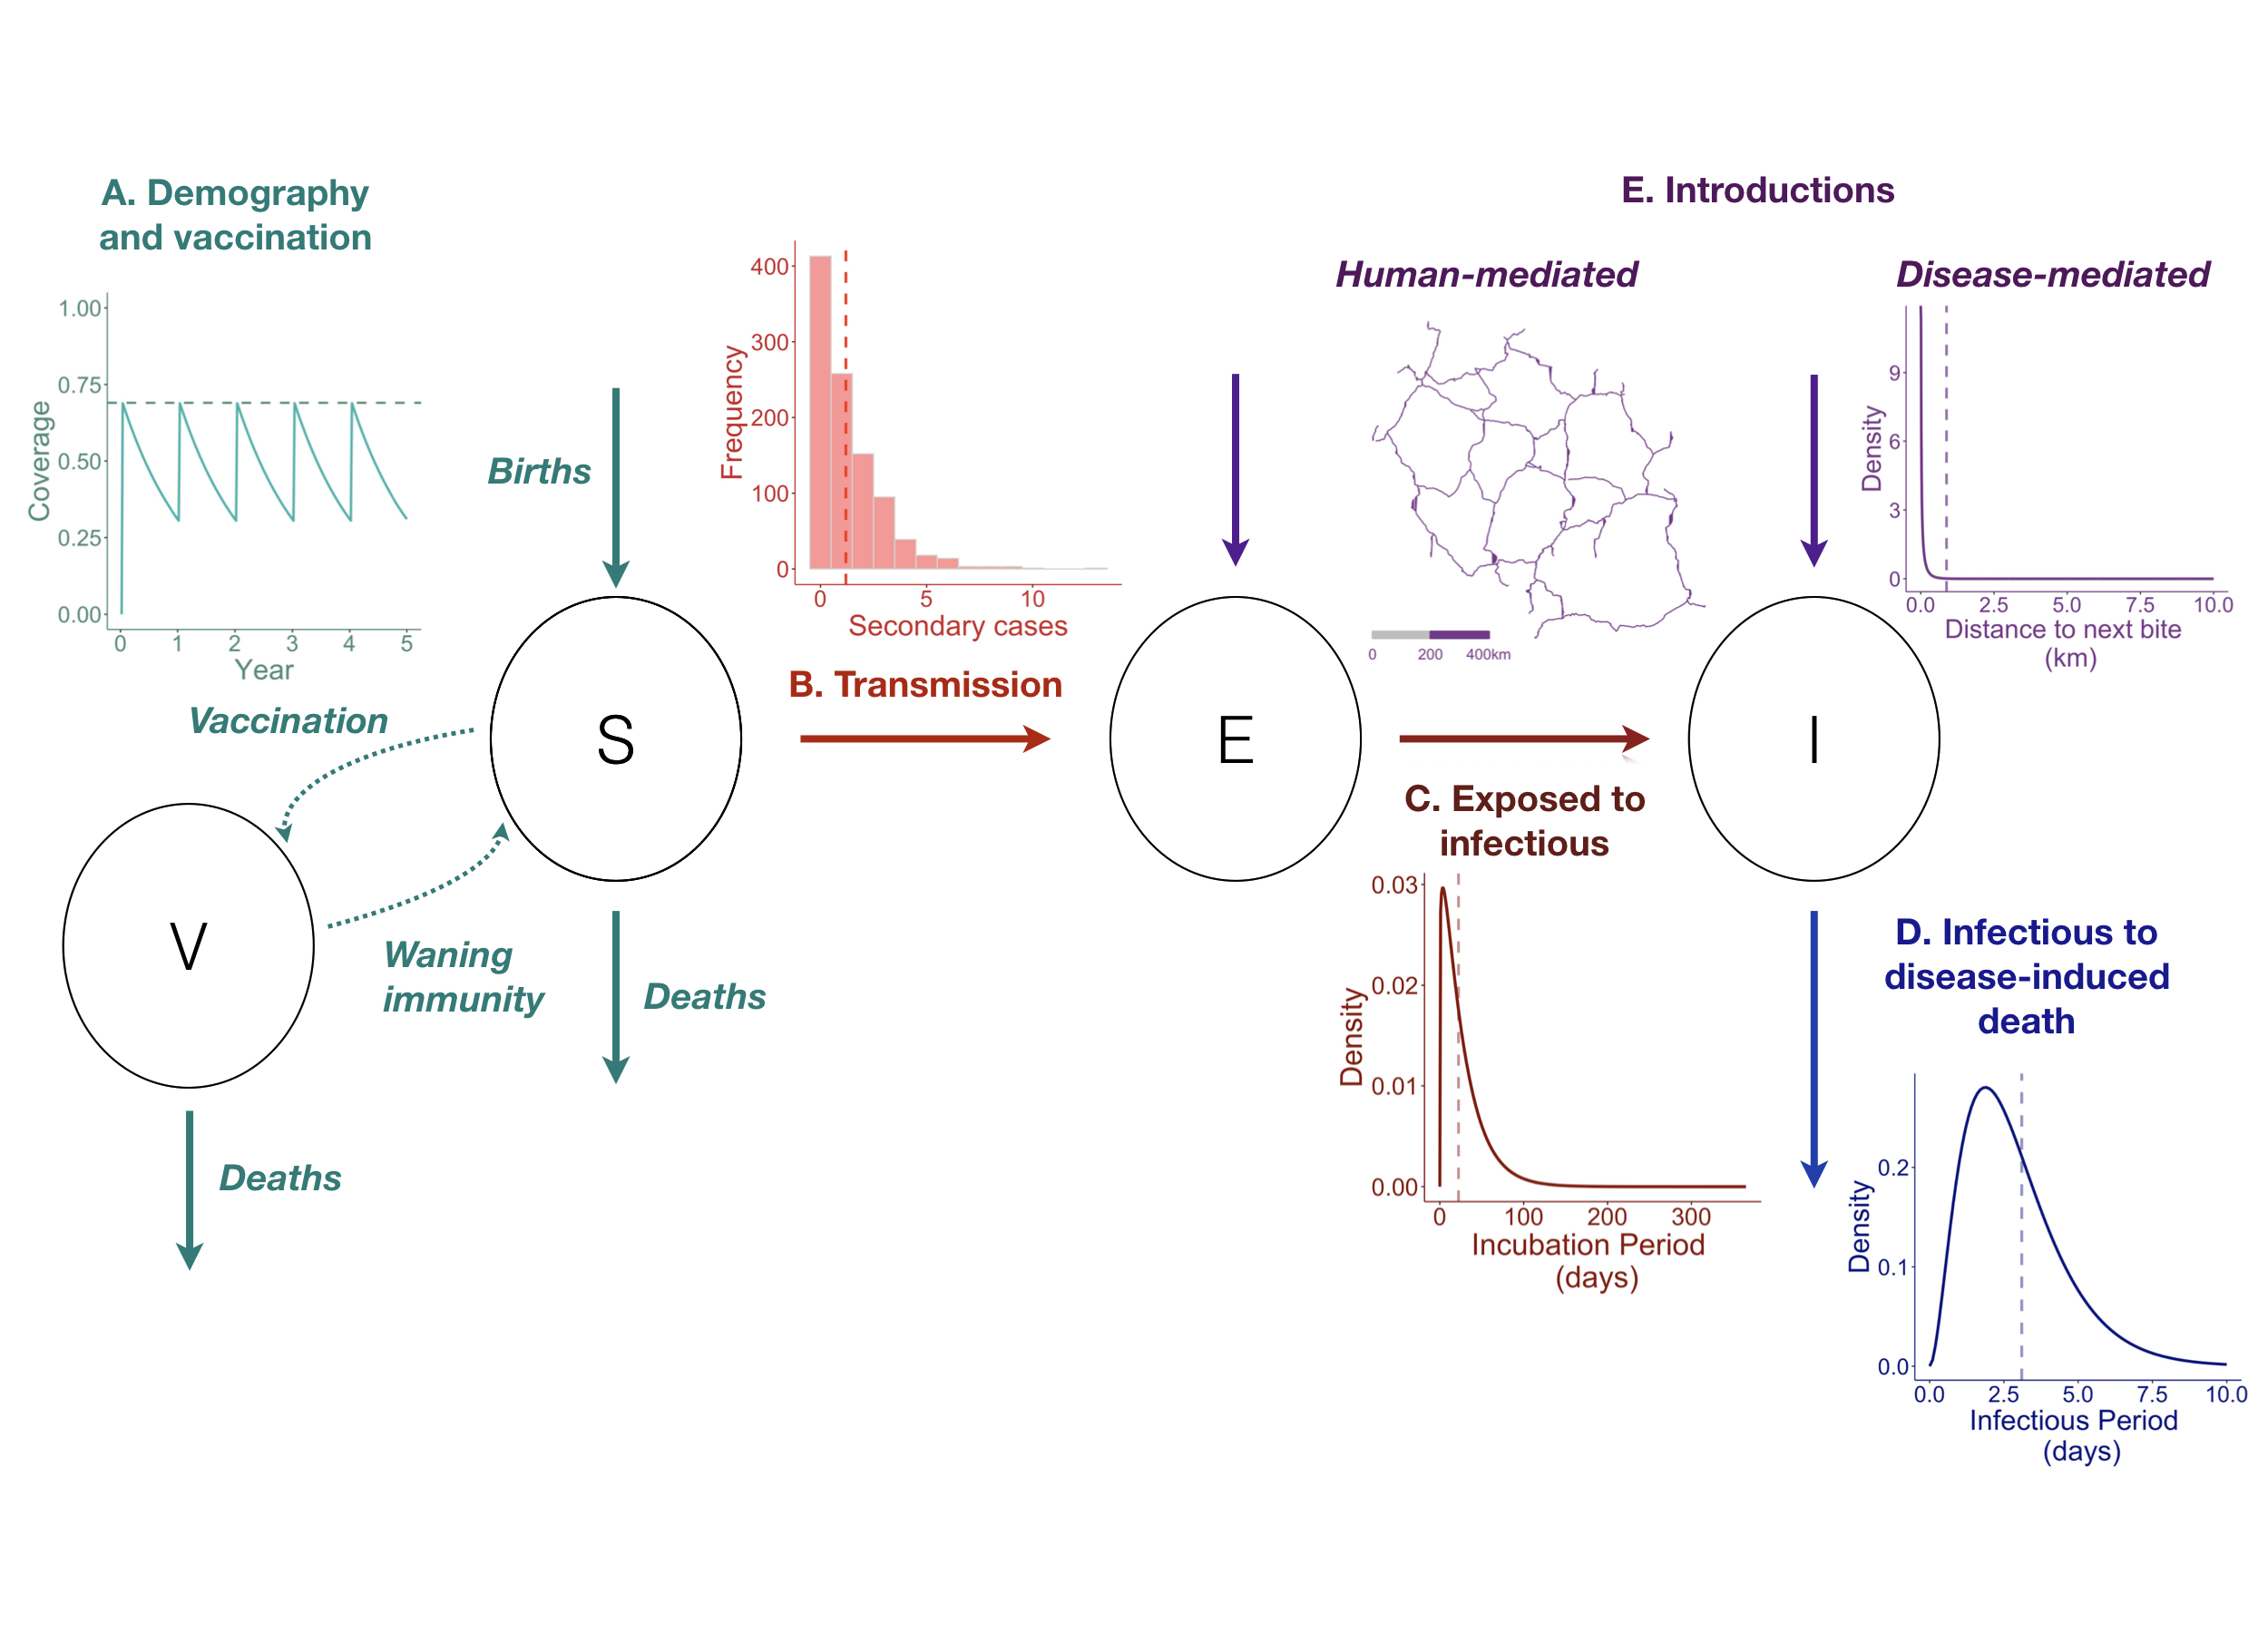
\includegraphics[width=0.9\linewidth]{figs/ch3/image1} \caption[The Susceptible-Exposed-Infectious-Vaccinated (SEIV) modeling framework for canine rabies.]{The Susceptible-Exposed-Infectious-Vaccinated (SEIV)
modeling framework for canine rabies: circles indicate epidemiological
classes, arrows linking circles indicate how individuals can move
between classes, insets describe underlying processes and influences.
\textbf{A) Host demography (i.e., the balance between births and deaths) and
vaccination} govern the susceptible and vaccinated population dynamics.
Following vaccination campaigns, vaccination coverage (y axis, inset)
first increases (vertical jumps) then wanes over time (x axis) as
vaccinated individuals die, susceptible individuals are born, or as
immunity conferred by vaccination wanes (in this example, campaigns
reach 70\% of the population annually, but coverage wanes to
approximately 35\% before the next annual campaign). \textbf{B) Transmission}
is on average low, but highly heterogeneous. Inset shows number of
secondary cases generated from a negative binomial distribution (n =
1000 draws, mean number of secondary cases = 1.2, red dashed line).
\textbf{C)} Individuals move from \textbf{exposed to infectious} on average after
22.3 days (inset, dashed line) but this is also highly variable with
some infections occurring months to years after exposure. \textbf{D)
Disease-induced mortality} is complete, and the infectious period is
short, on average 3.1 days (dashed line), with deaths due to infection
occurring within 10 days. \textbf{E) Introductions} from outside the
population modeled may seed cases within. Introductions may results from
\textbf{disease-mediated} movement of infectious dogs (sometimes upwards of
10 km; inset shows dispersal kernel, gamma distribution) and
\textbf{human-mediated} movements of incubating dogs (potentially on the
scale of 100s of km through movement along roads; the inset shows an
example of a major road network in Tanzania). All parameters used and
associated references are listed in Table \ref{tab:ch4-tab1}}\label{fig:ch4-fig1}
\end{figure}






























\begin{longtable}[]{@{}
  >{\raggedright\arraybackslash}p{(\columnwidth - 10\tabcolsep) * \real{0.17}}
  >{\raggedright\arraybackslash}p{(\columnwidth - 10\tabcolsep) * \real{0.34}}
  >{\raggedright\arraybackslash}p{(\columnwidth - 10\tabcolsep) * \real{0.21}}
  >{\raggedright\arraybackslash}p{(\columnwidth - 10\tabcolsep) * \real{0.05}}
  >{\raggedright\arraybackslash}p{(\columnwidth - 10\tabcolsep) * \real{0.17}}
  >{\raggedright\arraybackslash}p{(\columnwidth - 10\tabcolsep) * \real{0.05}}@{}}
\caption{\label{tab:ch4-tab1} Key parameter values associated with underlying processes illustrated in \ref{fig:ch4-fig1}.}\tabularnewline
\toprule
Process & Distribution & Parameters & Value & Source & Inset \\ \addlinespace
\midrule
\endfirsthead
\toprule
Process & Distribution & Parameters & Value & Source & Inset \\ \addlinespace
\midrule
\endhead
Birth rate & -- & Mean annual rate (dogs/yr) & 0.5 & {[}20{]} & A \\ \addlinespace
Death rate & -- & Mean annual rate (dogs/yr) & 0.42 & {[}20{]} & A \\ \addlinespace
Vaccine waning & -- & Mean annual rate (dogs/yr) & 0.33 & {[}10{]} & A \\ \addlinespace
Secondary cases (R0) & Negative binomial, mean 1.2 secondary cases & Mean & 1.2 & Townsend et al., 2013 & B \\ \addlinespace
& & Dispersion parameter (k) & 1.3 & & \\ \addlinespace
Incubation period & Gamma, mean 22.3 days & Shape & 1.15 & Hampson et al., 2009 & C \\ \addlinespace
& & Rate & 0.04 & & \\ \addlinespace
Infectious period & Gamma, mean 3.1 days & Shape & 2.9 & Hampson et al., 2009 & D \\ \addlinespace
& & Rate & 1.01 & & \\ \addlinespace
Dispersal kernel & Gamma, mean 0.88 km & Shape & 0.215 & Townsend et al., 2013 & E \\ \addlinespace
& & Rate & 0.245 & & \\ \addlinespace
\bottomrule
\end{longtable}

\hypertarget{how-to-model-rabies-virus-transmission}{%
\section{How to model rabies virus transmission?}\label{how-to-model-rabies-virus-transmission}}

There has been considerable debate about how to model rabies virus
transmission, which echoes a larger debate within the disease ecology
community {[}21{]}. Theory indicates that for diseases with
density-dependent transmission, i.e.~when transmission scales with host
density, there exists a threshold density below which the disease cannot
persist {[}22{]}. However, there is no such threshold when transmission is
frequency-dependent, i.e.~transmission rates are independent of host
density {[}21{]}.

For canine rabies, the basic reproductive number (\emph{R\textsubscript{o}}) or the average
number of secondary cases resulting from a single infection in a
completely susceptible population, is generally estimated as between 1-2
{[}14{]}, {[}23{]}-{[}25{]}. Such consistently low estimates of R\textsubscript{0} across a
range of dog densities suggest that rabies virus transmission is largely
frequency-dependent {[}14{]}, {[}24{]}, {[}26{]}-{[}28{]}. That is, rabid dogs
have on average the same number of infectious contacts regardless of the
density of dogs around them. As a result, reductions in population
densities are not likely to be effective in eliminating rabies. In
practice, although a common practice and one predicated on assumptions
of density-dependent transmission, indeterminate culling of dogs does
not curtail rabies transmission {[}29{]}.

Despite evidence for frequency-dependent transmission, many modeling
studies formulate rabies transmission as density-dependent (Fig \ref{fig:ch4-fig2}D). For a given R\textsubscript{0}, this assumption of density-dependent
transmission does not impact herd immunity thresholds; the critical
proportion that needs to be vaccinated, p\textsubscript{c}, is equal to 1 - 1/R\textsubscript{0}
regardless of the form of transmission {[}22{]}. However density-dependent
models predict reductions in transmission due to declining dog density
(e.g., via culling or disease-induced mortality) that are unlikely to
translate to the real world.

Models with frequency-dependent transmission are also not entirely
consistent with empirical observations. Frequency-dependent models that
assume homogeneous mixing (i.e.~equal contact probabilities between all
individuals in a population, also referred to as `mass action') result
in eventual population extinction for fatal pathogens like rabies
{[}30{]}. Only under very low transmission (1.01-1.02) and high population
growth can rabies persist in models with frequency-dependent
transmission. For models with density-dependent transmission, even with
R\textsubscript{0} between 1.01 and 1.1, models of rabies show high annual incidence
(Figure \ref{fig:figS1}), which is at odds with empirical evidence. Where
measured, rabies incidence is low (\textless{} 1-2\% annually) and consequently
has little demographic impact on dog populations {[}31{]}. Additional
model structure is therefore necessary to explain how rabies can persist
at such low incidence.

Transmission heterogeneity may be a potential mechanism to explain the
relatively low incidence of rabies. A high proportion of dead-end or
singleton transmissions result in negligible depletion of susceptibles,
while occasional super-spreaders may seed and maintain transmission. In
addition to unrealistic estimates of rabies incidence, if heterogeneity
in transmission is not captured, there is a risk that models may
generate biased estimates of control indicators, such as the time to
elimination and the threshold level of vaccination that this requires.

Accounting for the spatial scale of transmission could also explain how
rabies persists at low incidence. As most transmission occurs within a 1
km radius of infected animals, susceptible depletion at such fine scales
may limit transmission in a way that is not captured in mass action
models {[}32{]}. Phenomenological approximations may offer a solution to
this challenge {[}33{]}, {[}34{]}, but have yet to be thoroughly explored
for rabies. Spatially-explicit individual-based models implemented at
the scale at which most mixing occurs generate more realistic dynamics
{[}24{]}, {[}35{]}, but are computationally intensive and not analytically
tractable. Nonetheless, such models provide insights into underlying
mechanisms that could be simplified for more expedient models. Finally,
human behavior has also been implicated in curtailing epidemics, with
responses such as tying and killing infectious dogs and reactive
vaccination thought to scale with incidence {[}36{]}.

There is limited data to disentangle these potential mechanisms, which
could reconcile empirical observations with modeling results. Further
work is necessary to ensure sufficient model realism to inform policy,
but balancing realism and complexity is a key challenge for any modeling
study {[}37{]}. Building in realism requires additional parameterization
and, often, additional assumptions. Robust epidemiological and
biological data are therefore key to improving our understanding of how
to model rabies transmission.

\begin{figure}
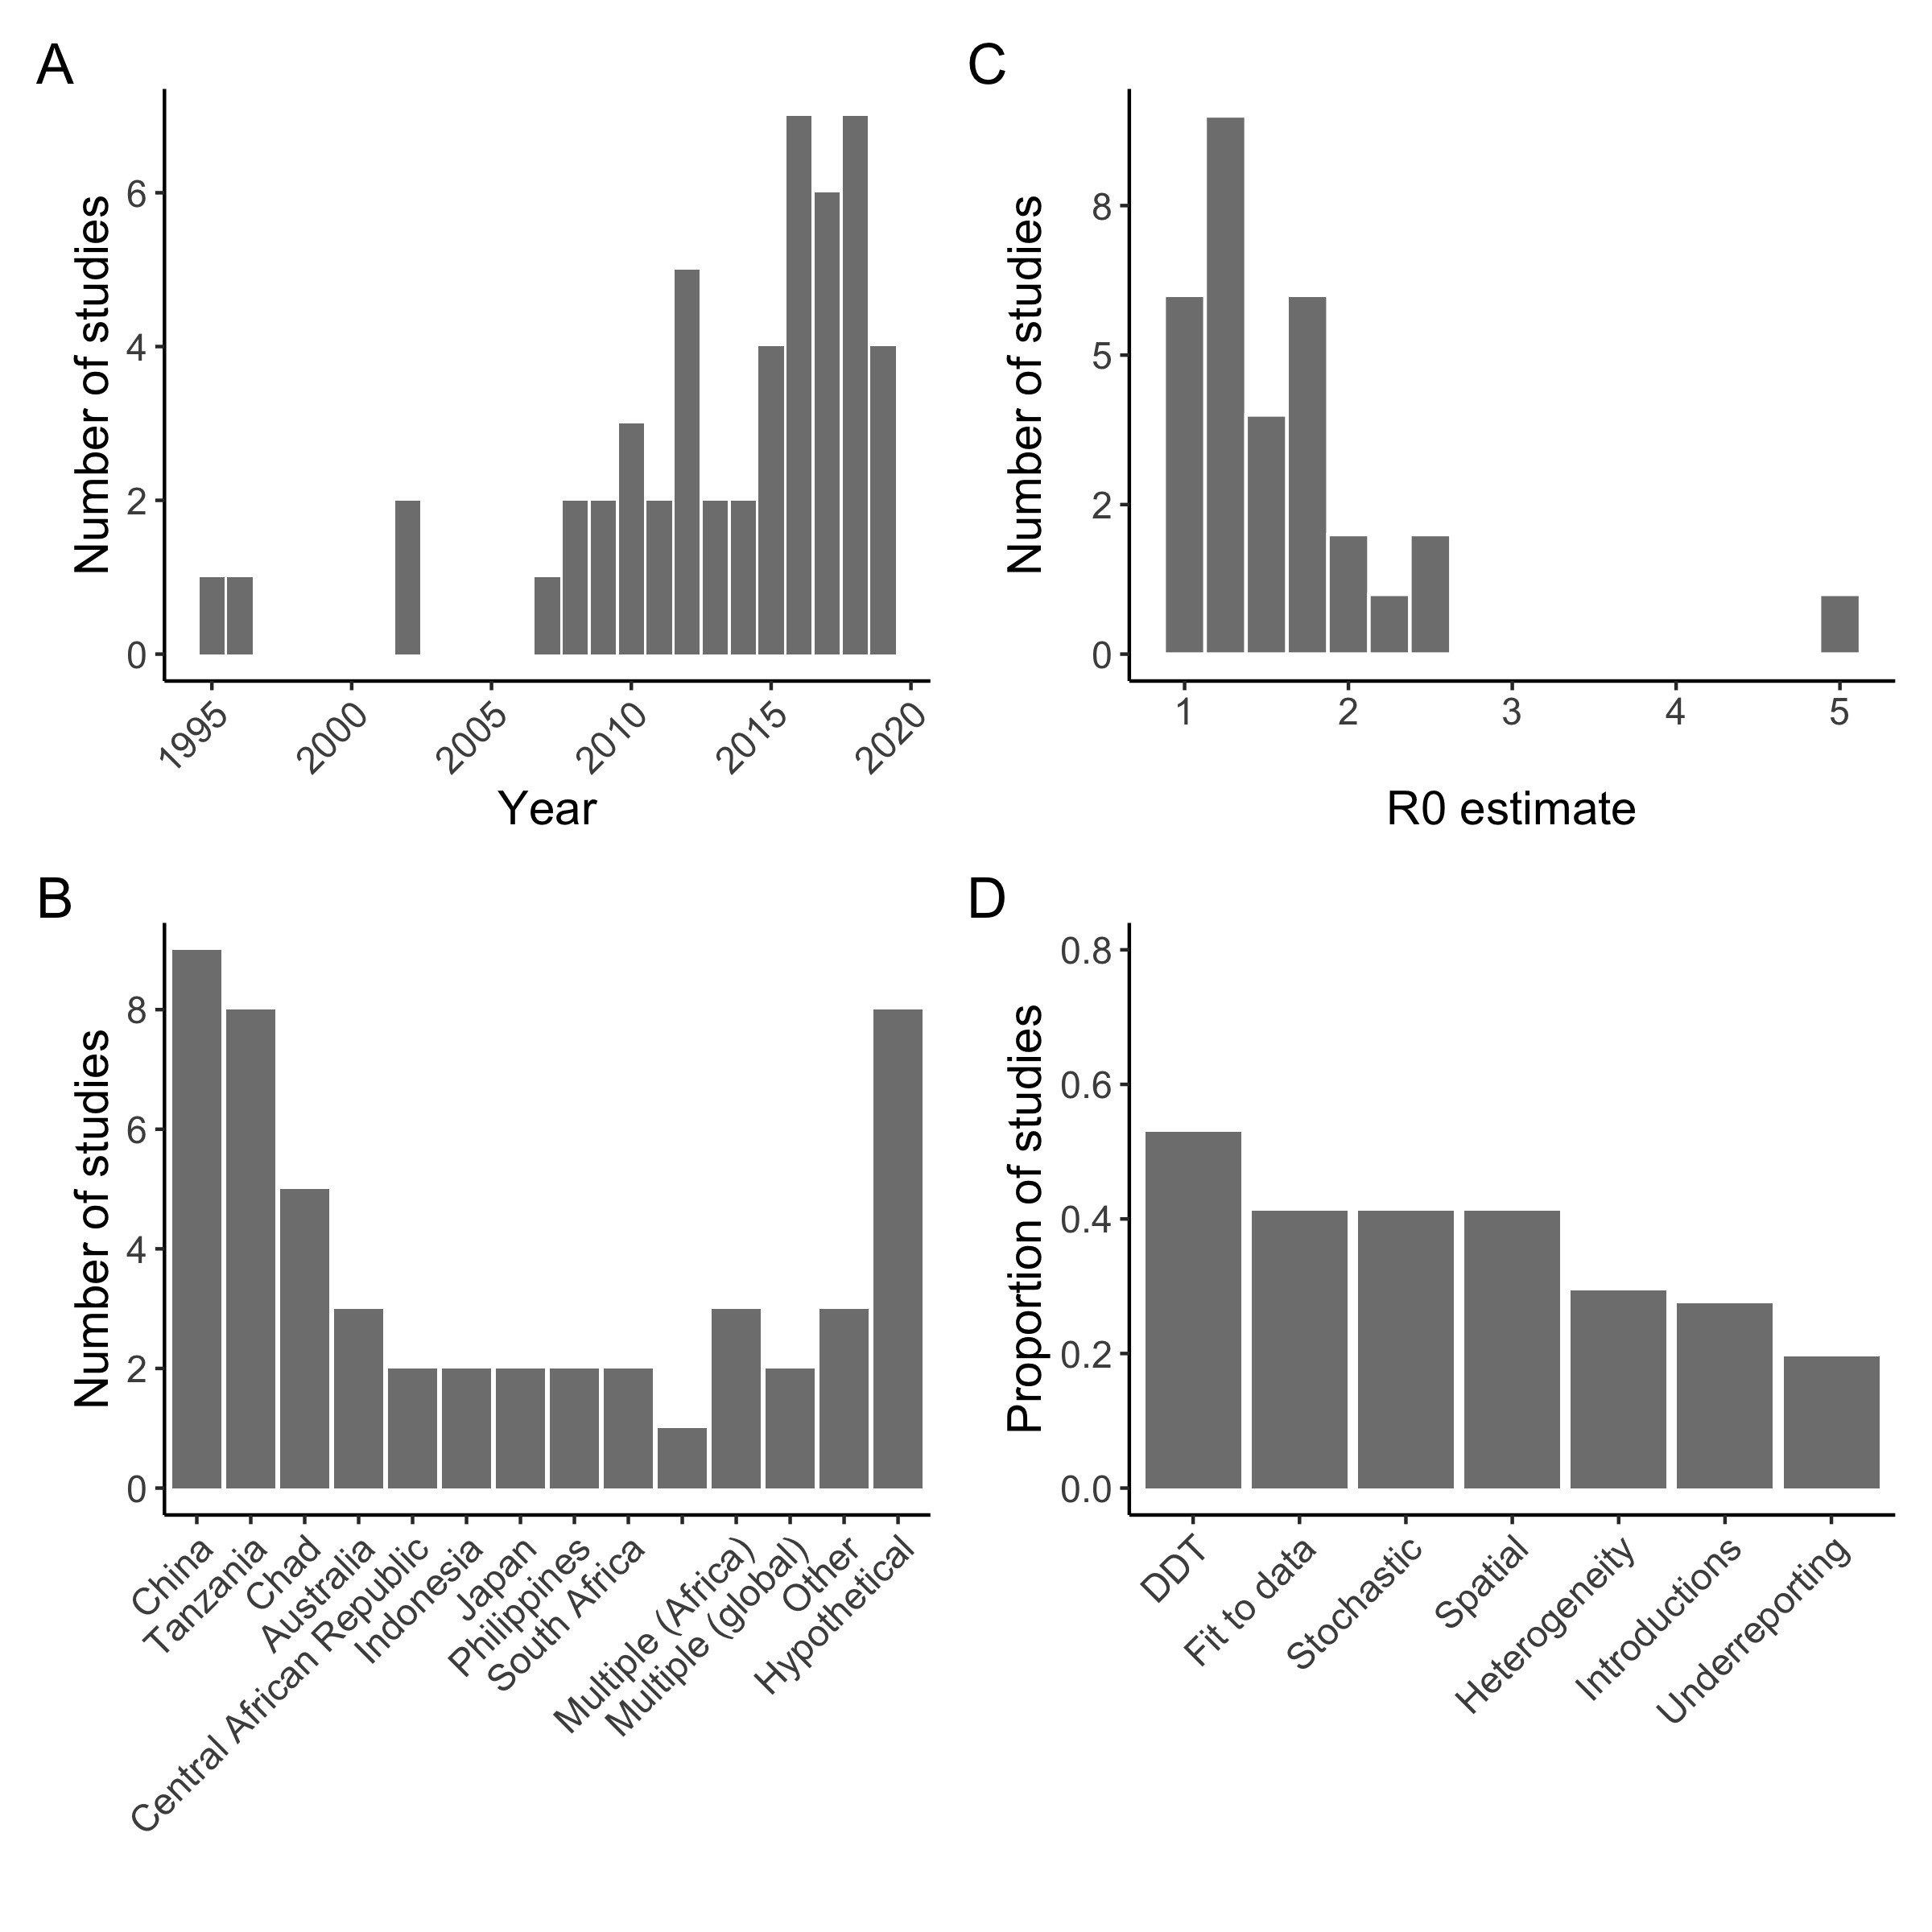
\includegraphics[width=0.9\linewidth]{figs/ch3/image2} \caption[Summary of studies with a dynamic model of canine rabies.]{Summary of studies with a dynamic model of canine
rabies. A total of 51 studies were included. A) Year of publication,
with most studies published after 2006; B) Countries where rabies
dynamics were modeled: studies were concentrated in China, Tanzania, and
Chad, but many also examined dynamics in hypothetical contexts, not
specific to any geographic situation. C) Estimates of R\textsubscript{0}: most studies
estimated R\textsubscript{0} below 2 (10 studies, with 31 estimates; estimates of R\textsubscript{e}
(the effective reproduction number which accounts for ongoing
vaccination) and R\textsubscript{t} (time-varying reproductive number) were excluded
(N = 3). D) Key features of models (N = 51): most assumed
density-dependent transmission (N = 27). Less than half were fit to data
(N = 20), stochastic (N = 20), or spatially-explicit (N = 19). 15/51
studies incorporated individual heterogeneity in transmission and 14/51
introductions from outside the population modeled. Only 10 included an
observation model in their analysis or accounted for under-reporting in
their inference. Full bibliography and metadata included in
Supplementary Table 1.}\label{fig:ch4-fig2}
\end{figure}



















\hypertarget{existing-modeling-studies}{%
\section{Existing Modeling Studies}\label{existing-modeling-studies}}

Two systematic reviews of rabies models recently examined the
effectiveness and cost-effectiveness of control and prevention
strategies. They concluded that estimates of R\textsubscript{0} are consistently below
2 and dog vaccination is an effective strategy, but vaccination coverage
is critically influenced by dog demography {[}38{]}. Both mass dog
vaccination and provisioning of PEP to bite patients are cost-effective,
in contrast to dog culling which has rarely been identified as either
economically feasible or effective {[}39{]}. Building off these reviews,
we examined studies with a dynamic modeling component and synthesized
insights generated and data used to inform them. We searched for papers
that had the terms ``rabies'' AND (``domestic dog*'' OR ``canine'') AND
``model*'' on PubMed and Scopus, including all English language papers
published between January 1995 and July 2019 that incorporated a
transmission model of rabies virus in domestic dogs. Of the 547 unique
records retrieved, 51 papers fitted these inclusion criteria (Fig
\ref{fig:ch4-fig3}, Online Supplementary Table S1).

\hypertarget{insights-and-limitations}{%
\subsection{Insights and limitations}\label{insights-and-limitations}}

Of studies that compared intervention strategies (generally: mass dog
vaccination, human PEP provisioning, and dog population control
including culling), the majority show that dog vaccination is most
effective, and essential to achieve elimination. Despite the potential
to maximize population-level immunity, synchronizing vaccination
campaigns geographically had little impact on probability of
elimination, at least for annual vaccination campaigns. In contrast,
spatial heterogeneity in vaccination coverage had a greater impact, with
even small contiguous coverage gaps reducing the probability of rabies
being eliminated {[}24{]}, {[}35{]}.

While the critical vaccination threshold (\emph{p\textsubscript{c}} or 1 - 1/\emph{R\textsubscript{o})} should
theoretically be much lower than 70\% for a disease with the low range of
R\textsubscript{0} estimated for rabies (Figure \ref{fig:ch4-fig2}C), the coverage level recommended
by WHO reflects an empirical consensus {[}23{]}, {[}40{]}. Models show that
due to high turnover in domestic dog populations, annual campaigns that
reach at least 70\% of the population are necessary to maintain coverage
\textgreater{} 20\% throughout the year. Furthermore, heterogeneity in transmission
and frequent introductions of rabies cases increase both the vaccination
threshold necessary to interrupt transmission, and the probability of
observing small outbreaks even when vaccination coverage is high {[}14{]},
{[}41{]}.

Most published models were deterministic (33/51) and did not incorporate
heterogeneities in transmission (36/51, Figure \ref{fig:ch4-fig2}D). However, as R\textsubscript{0}
for rabies appears to be low, the interaction between stochasticity and
heterogeneity in transmission may be influential. In general, for
diseases with high transmissibility (i.e.~measles), heterogeneities in
transmission can often be ignored as these complexities have little
impact on the emergent dynamics of infection {[}30{]}. However, for a
disease with lower transmission, heterogeneities may result in
unpredictable outbreaks {[}37{]}. Stochasticity is especially crucial in
the endgame, when elimination probabilities and incursion dynamics
depend on rare events.

Most studies model rabies virus transmission in a closed population,
that is without introductions from neighboring areas (Figure \ref{fig:ch4-fig2}D).
While this is a reasonable approach in island settings such as in Bali,
Indonesia {[}24{]}, recent modeling and phylogenetic work shows the
importance of incursions in less isolated populations in sustaining
rabies virus transmission (Bourhy et al., 2016; Zinsstag et al., 2017)
and that multiple strains co-circulate within a population {[}42{]},
{[}43{]}. Human behavior is also a key driver of transmission patterns,
facilitating as well as dampening transmission {[}44{]}. Multiple studies
have found signals of long distance transmission beyond the range of
disease-mediated dispersal, showing the role of human-mediated movement
of incubating dogs {[}44{]}-{[}46{]}. Road networks have been identified as
correlates of phylogenetic distance, indicating that human movement
could shape the spatial structure of canine rabies virus {[}44{]}-{[}46{]}.
There is also strong pyhlogenetic evidence that historical
human-mediated long-distance movements underlie much of the contemporary
global distribution of canine rabies {[}47{]}. This work emphasizes the
need to understand how the size and connectivity of populations affects
the persistence of disease. Models have productively explored this
historically important question for childhood infections such as measles
{[}48{]}, but for canine rabies, this remains an important challenge,
which may well define progress towards elimination.

A few studies look at how contact networks and movement behaviors could
drive transmission {[}49{]}-{[}51{]}. These studies simulated outbreaks on
contacts networks constructed using data from healthy domestic dogs.
They found that in general, targeting highly connected dogs or dogs with
larger home ranges for vaccination results in a higher probability of
disease elimination, but few predictors of connectivity of individuals
emerged. Broadly, these results are consistent with previous work on
transmission heterogeneity and could bring valuable benefits if it were
possible to \emph{a priori} identify and target high-risk animals. However,
these traits are difficult to estimate in most endemic settings, where
there is limited data on dog populations, let alone individual dog
traits. Moreover, as rabies causes severe neurological symptoms, the
validity of these findings depends on how representative data from
healthy dogs are of movement and contact patterns of rabid dogs.

Dynamic models have been integrated with economic models to estimate
cost-effectiveness of interventions, demand for rabies PEP, and disease
burden. Early cost-effectiveness models critically lacked data on the
costs of PEP for those seeking care for non-rabid dog bites {[}27{]},
{[}52{]}, {[}53{]}. Decision tree models have addressed these issues and
provide a framework to integrate field data on rabies exposures,
health-seeking, and access and adherence to PEP into estimates of burden
{[}54{]}-{[}56{]}. These more recent studies demonstrate that PEP is still a
very cost-effective intervention even when accounting for management of
patients bitten by non-rabid animals and emphasize the potential value
of administering rabies vaccine intradermally using the latest WHO
recommended abridged regimens {[}57{]}. However, they also highlight two
other critical points for policy. First, without strategies for more
judicious use, costs of PEP will remain high and continue to rise even
when dog rabies is controlled. Moreover, human rabies deaths will
continue to occur and the target of zero deaths by 2030 cannot be
achieved through PEP alone. A massive scaling up of dog vaccination is
required in most endemic countries. Support for human rabies vaccines
through Gavi, the Vaccine Alliance, is therefore a promising step
towards the 2030 goal {[}56{]}, but more investment and commitment is
still needed.

\begin{figure}
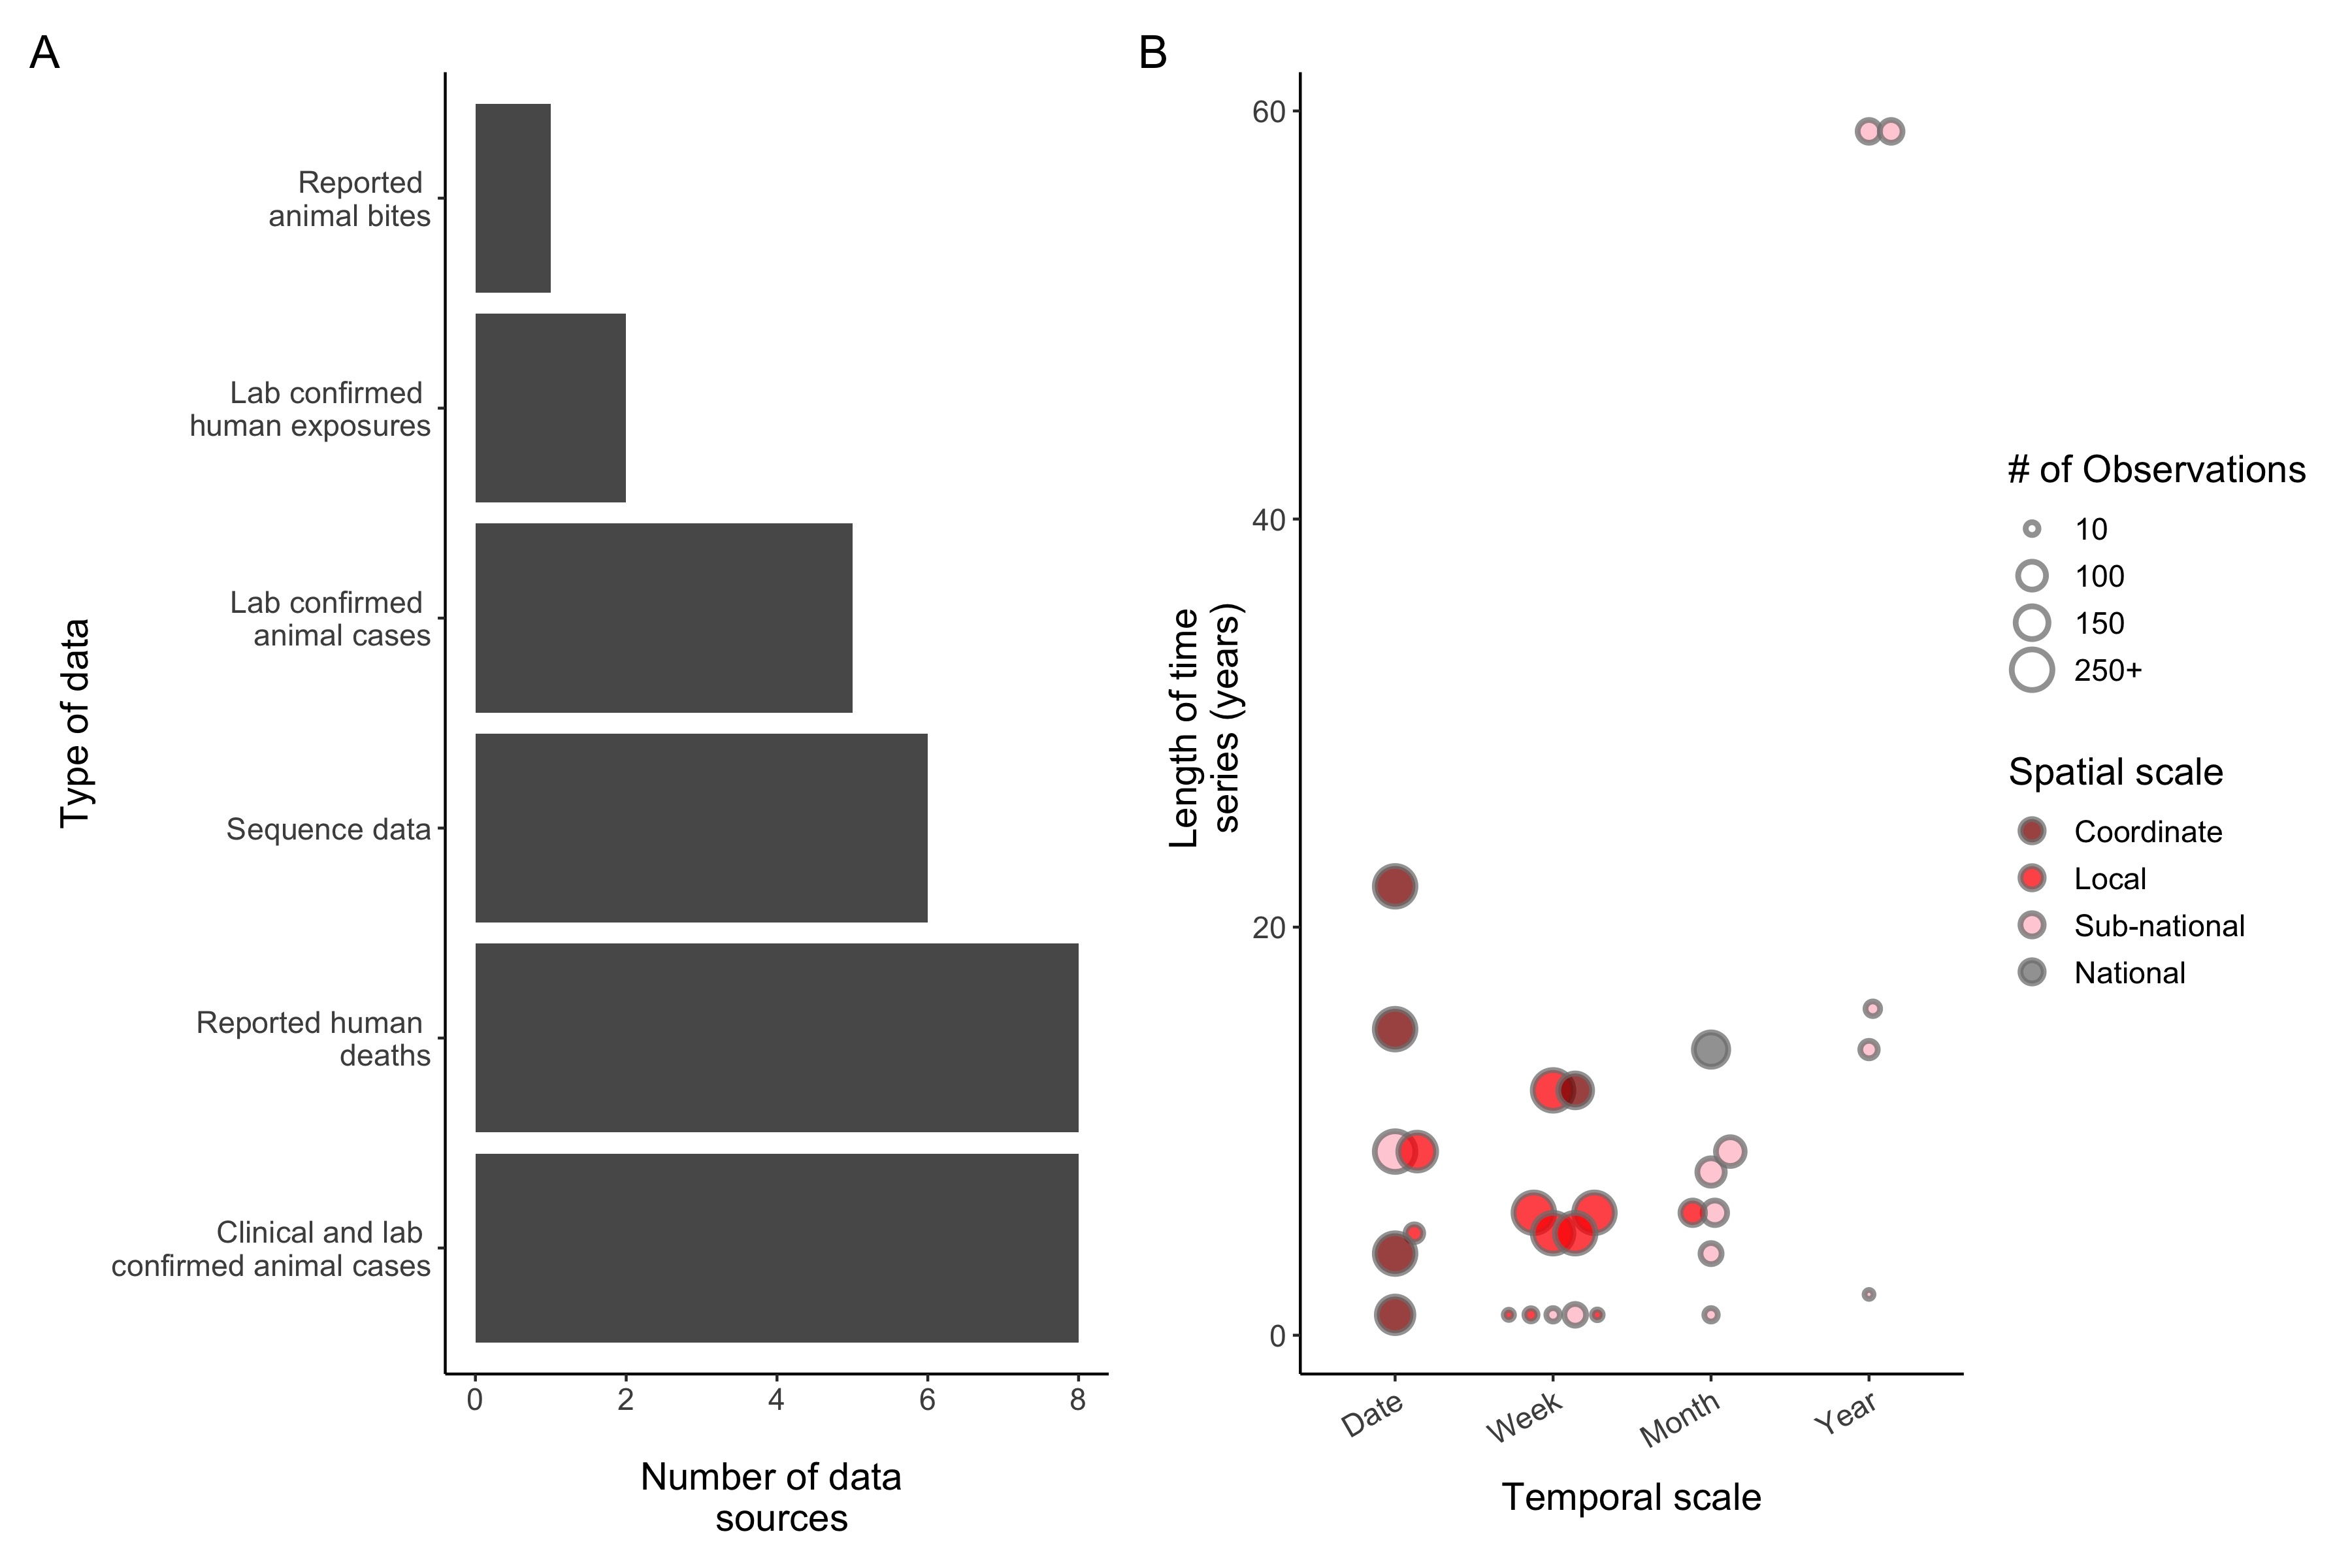
\includegraphics[width=0.9\linewidth]{figs/ch3/image3} \caption[Rabies data reported in modeling studies (N = 25 studies reporting 30 unique data sources).]{Rabies data reported in modeling studies (N = 25
studies reporting 30 unique data sources). A) Type of data used. B)
The scales of temporal (x-axis) and spatial (colors) information
available and the duration (y axis). The size of the points is
proportional to the number of observations in each data set. Any rabies
data that was reported in studies were included (even if not used for
fitting purposes, only for qualitative comparison). If multiple data
sets were used, they were included as separate data sources, and if the
same data set was used in multiple studies it was only included once.}\label{fig:ch4-fig3}
\end{figure}











\hypertarget{the-gap-between-models-and-data}{%
\section{The gap between models and data}\label{the-gap-between-models-and-data}}

Despite limited surveillance, few studies incorporated observation
models into their analyses or conducted sensitivity analyses on how
under-reporting might bias their inferences (Figure \ref{fig:ch4-fig2}D). Developing
models of the observation process and integrating them into dynamic
models (often termed state-space modeling, {[}58{]}-{[}60{]} is essential
when fitting to incomplete data. But, these modeling frameworks can also
guide surveillance strategies across the elimination timeline by
estimating the minimum detection levels and time necessary to verify
elimination {[}61{]}.

A major limitation of many existing modeling studies is a lack of data
to inform conclusions, with less than 40\% of models fit to data (Fig \ref{fig:ch4-fig2}D). For studies which did report incidence data, the scale and
quality of the data also varied greatly. Human deaths reported at the
national or regional level and numbers of clinical and laboratory
confirmed animal cases were the most commonly used data (Figure \ref{fig:ch4-fig3}A).
The number of observations and length of the time series varied greatly,
from over 1000+ observations at a fine spatiotemporal scale over a
15-year period to annual cases reported for only 2 years (Figure \ref{fig:ch4-fig3}B).
Ultimately, integrating data on rabies incidence and dog populations
into models of transmission is a critical step to moving modeling
efforts forward. Below we describe the various data sources that can be
used to fit and inform models and associated challenges and solutions to
collecting this data.

\hypertarget{bite-data}{%
\subsection{Bite data}\label{bite-data}}

Bite data, (i.e.~data on patients seeking care for animal bites) are
often used as a proxy for rabies exposure incidence. However, these data
often lack details on the status of the biting animal and are heavily
skewed by who has access to care, both geographically and
socioeconomically. Paradoxically, in settings where the direct cost of
PEP is charged to patients, bite records may be more reflective of
rabies exposures: people may be less likely to seek care when the
perceived risk is low (i.e.~fewer people seek care for provoked bites by
known healthy and/or vaccinated animals) due to the associated costs
{[}62{]}, {[}63{]}. In settings where PEP is provided for free and
indiscriminately, a higher proportion of reported bites may be due to
non-rabid animals {[}64{]}-{[}66{]}, and many Category 1 exposures, i.e.
those for which PEP is not indicated {[}67{]}, receive unnecessary PEP
{[}66{]}, {[}68{]}, {[}69{]}.

For data on bite patients to be more useful for modeling and
surveillance purposes, supplementary information for each bite beyond
the date reported and number of doses received is needed. Categorizing
the type of exposure per the WHO categories can help to exclude Category
1 exposures. Reporting clinical signs and the outcome of the biting
animal at each patient visit can identify probable rabies exposures and
trigger field investigations and sample collection to improve
surveillance. Finally, information on the geographical location where
the patient was bitten, for example to the finest scale administrative
unit identifiable, could be used to understand spatial patterns of
transmission, estimate demand for PEP, and identify determinants of
health seeking behavior.

\hypertarget{laboratory-confirmed-case-data}{%
\subsection{Laboratory confirmed case data}\label{laboratory-confirmed-case-data}}

Laboratory confirmed case data are considered a gold standard due to the
high sensitivity and specificity of diagnostic tests for rabies, but
represent the tip of the iceberg in terms of true incidence {[}9{]},
{[}61{]}. Diagnostic confirmation of rabies cases is often lacking in many
endemic settings due to limited laboratory and field capacity. Even with
strong laboratory resources in country, collecting a brain sample from a
suspected rabid animal or human case can be challenging. Lack of cold
chain and accessibility to communities, limited veterinary capacity and
training in euthanasia and sampling methods, and low reporting of
suspected cases are all significant barriers to case confirmation. For
humans, nuchal samples can be collected non-invasively (from nape of the
neck) to confirm a rabies case ante-mortem {[}70{]}. However, confirmation
of a human case first requires a person to seek care, and rabies deaths
are most common in populations with the least access to health care
{[}71{]}. For animal cases, field sample collection methods, like the
straw method of sampling brain tissue that does not require the
submission of the whole head, and alternative forms of sample storage
and testing, such as rapid diagnostic tests and filter papers, have
potential to address some of these challenges {[}72{]}. While these
alternative tests may not be appropriate for guiding patient treatment,
they could greatly improve surveillance and understanding of rabies
virus transmission if implemented more routinely.

Even with the gold-standard diagnostic test, using laboratory
confirmation to guide administration of PEP in endemic settings may be
impractical, due to delays in sampling and testing. Integrated bite case
management (IBCM, see Chapter 18) programs, which combine risk
assessments, field investigations, animal observation/quarantine, and
sampling of suspected cases, are a promising method of improving rabies
surveillance and PEP provisioning. IBCM can increase both detection of
and confirmation of clinically suspect animal cases and guide referrals
for PEP , as well as limit further exposures by euthanizing rabid
animals once detected {[}73{]}. However, IBCM relies on coordination
between human and animal health practitioners and resources to support
clinical rabies diagnosis and field sample collection, which is still
lacking in most low-income countries.

\hypertarget{sequence-data}{%
\subsection{Sequence data}\label{sequence-data}}

Sequence data can be used to make inferences about transmission
processes, particularly when linked with epidemiological data
{[}43{]}-{[}45{]}, {[}60{]}, {[}74{]}, {[}75{]}. Recent studies have demonstrated
the added value of whole-genome sequencing (WGS) for understanding finer
scale transmission dynamics of canine rabies {[}44{]}, {[}74{]}, but WGS has
yet to be routinely generated for canine rabies. Sequencing capacity is
even more limited than general laboratory capacity in rabies-endemic
countries and exporting samples for sequencing is costly. Advances in
portable, real-time sequencing could help to tackle these limitations in
the field (ARTICnetwork, \url{http://artic.network/index.html}). Portable
sequencers such as the MinION could support rapid generation and
dissemination of sequence data. Methods to sequence from alternative
sample types, such as rapid diagnostic tests and filter papers, could
also help to overcome obstacles in field sample collection and transport
{[}72{]}. Bioinformatic pipelines and open sharing of sequences, such as
those developed for other viral pathogens {[}76{]}, could greatly
facilitate our understanding of rabies dynamics at a regional and global
scale. In general, low-cost, high-throughput sequencing methods should
be developed to increase the timely availability of representative
sequence data from endemic settings.

\hypertarget{dog-population-and-vaccination-data}{%
\subsection{Dog population and vaccination data}\label{dog-population-and-vaccination-data}}

Data on the dog population is necessary to further understand how the
distribution, density, and connectivity of the host population drives
transmission {[}74{]}. Estimates of vaccination coverage and other
intervention efforts facilitate inference of the mechanisms driving
transmission and the impact of interventions, helping to predict future
outcomes given different control strategies {[}75{]}. In most endemic
countries, limited systematic data is collected on dog populations. If
integrated into more routine census or demographic surveys (i.e.~the
Demographic and Health Surveys, \url{https://dhsprogram.com}), questions on
dog ownership and vaccination status at the household level could be a
potential way to get this data where the majority of the dog population
is owned. However, if conducted as standalone surveys, these can be
resource intensive and difficult to implement in a representative way,
particularly in more rural/remote areas. Alternatively, integrating
post-vaccination coverage surveys into campaigns has been shown to be a
cost-effective way to generate coverage and population estimates, and
only requires temporary marking of vaccinated dogs {[}77{]}-{[}79{]}. As
spatial heterogeneity in coverage is likely a key factor driving the
success of vaccination campaigns, such coverage estimates at the scale
at which campaigns are implemented could be critical to understanding
rabies persistence and elimination probabilities.

\hypertarget{conclusions}{%
\section{Conclusions}\label{conclusions}}

Modeling studies, in combination with decades of empirical evidence,
have demonstrated that dog vaccination is the optimal intervention
strategy for controlling canine rabies. As global momentum for
implementing national rabies control programs grows, models should move
beyond comparing vaccination and other strategies in idealized
populations towards linking models with field data to identify
refinements to intervention strategies. To date, most work has focused
on studying control efforts and identifying drivers of dynamics (often
without using data), and studies of the impact of control have rarely
been linked to analyses grounded in empirical data (i.e.~studies that
explained observed patterns or estimated key parameters, see
Figure \ref{fig:figS2} for an overview of existing studies). Models
should aim to integrate these questions and test specific vaccination
strategies, such as ring vaccination or establishment of control
corridors based on geographic barriers as implemented for wildlife
rabies in Europe.

Key parameters to estimate from models and data include transmission
heterogeneity (captured in the distribution of secondary cases), the
dispersal kernel, and introduction rates (including how to differentiate
ongoing local transmission from imported cases). Integrating models of
surveillance into dynamic models can further establish surveillance
requirements necessary to verify freedom from disease and inform policy
decisions regarding the cessation and scaling back of control efforts.
Importantly, models can predict how these requirements might change over
the elimination timeline. Given the challenges in generating
high-quality surveillance data for canine rabies, these models can also
be used to account for under-reporting and determine the minimum level of
detection necessary for robust inference. Phylodynamic approaches, which
combine both epidemiological and genetic data, are a promising avenue to
tackle many of these questions. Critically, progress in this area will
require strong surveillance systems and representative data from a range
of populations.

Countries have made varying progress towards elimination, ranging from
some that lack a realized national control policy and others in the
end-game stages of elimination. Now, we are tasked with building
flexible models that can capture rabies dynamics and the impacts of
control across the elimination timeline. Identifying where and how
implementation of control efforts needs improving and delivering such
improvements will require a much closer collaboration between
scientists, practitioners and policymakers.

\hypertarget{data-and-code-availability}{%
\section{Data and code availability}\label{data-and-code-availability}}

All data and code used to generate figures and supplemental files, as
well as the bibliography for the literature review are available online
at \url{https://github.com/mrajeev08/ModelingChapter}.

\hypertarget{references-3}{%
\section{References}\label{references-3}}

\setlength{\parskip}{1em}

{[}1{]} H. Heesterbeek, R. M. Anderson, V. Andreasen, S. Bansal, D. De Angelis, C. Dye, K. T. D. Eames, W. J. Edmunds, S. D. W. Frost, S. Funk, T. D. Hollingsworth, T. House, V. Isham, P. Klepac, J. Lessler, J. O. Lloyd-Smith, C. J. E. Metcalf, D. Mollison, L. Pellis, J. R. C. Pulliam, M. G. Roberts, C. Viboud, Isaac Newton Institute IDD Collaboration, ``Modeling infectious disease dynamics in the complex landscape of global health,'' Science, vol.~347, no. 6227, pp.~aaa4339--aaa4339, Mar.~2015.

{[}2{]} P. Klepac, C. J. E. Metcalf, A. R. McLean, and K. Hampson, ``Towards the endgame and beyond: complexities and challenges for the elimination of infectious diseases,'' Philosophical Transactions of the Royal Society B: Biological Sciences, vol.~368, no. 1623, pp.~20120137--20120137, Jun.~2013.

{[}3{]} V. G. Panjeti and L. A. Real, ``Mathematical models for rabies.,'' Adv. Virus Res., vol.~79, pp.~377--395, 2011.

{[}4{]} R. M. Anderson, H. C. Jackson, R. M. May, and A. M. Smith, ``Population dynamics of fox rabies in Europe,'' Nature, vol.~289, no. 5800, pp.~765--771, Feb.~1981.

{[}5{]} J. D. Murray, E. A. Stanley, and D. L. Brown, ``On the spatial spread of rabies among foxes,'' Proceedings of the Royal Society of London. Series B. Biological Sciences, vol.~229, no. 1255, pp.~111--150, Nov.~1986.

{[}6{]} D. L. Smith, B. Lucey, L. A. Waller, J. E. Childs, and L. A. Real, ``Predicting the spatial dynamics of rabies epidemics on heterogeneous landscapes.,'' Proc Natl Acad Sci USA, vol.~99, no. 6, pp.~3668--3672, Mar.~2002.

{[}7{]} S. M. Duke-Sylvester, L. Bolzoni, and L. A. Real, ``Strong seasonality produces spatial asynchrony in the outbreak of infectious diseases,'' Journal of The Royal Society Interface, vol.~8, no. 59, pp.~817--825, Jan.~2011.

{[}8{]} S. Cleaveland, H. Beyer, K. Hampson, D. Haydon, F. Lankester, T. Lembo, F.-X. Meslin, M. Morters, Z. Mtema, M. Sambo, and S. Townsend, ``The changing landscape of rabies epidemiology and control.,'' Onderstepoort J. Vet. Res., vol.~81, no. 2, pp.~E1--8, Apr.~2014.

{[}9{]} T. P. Scott, A. Coetzer, A. S. Fahrion, and L. H. Nel, ``Addressing the Disconnect between the Estimated, Reported, and True Rabies Data: The Development of a Regional African Rabies Bulletin,'' Front Vet Sci, vol.~4, no. 4, pp.~1--6, Feb.~2017.

{[}10{]} N. Lakshmanan, T. C. Gore, K. L. Duncan, M. J. Coyne, M. A. Lum, and F. J. Sterner, ``Three-year rabies duration of immunity in dogs following vaccination with a core combination vaccine against canine distemper virus, canine adenovirus type-1, canine parvovirus, and rabies virus.,'' Vet. Ther., vol.~7, no. 3, pp.~223--231, 2006.

{[}11{]} T. Lembo, D. T. Haydon, A. Velasco-Villa, C. E. Rupprecht, C. Packer, P. E. Brandão, I. V. Kuzmin, A. R. Fooks, J. Barrat, and S. Cleaveland, ``Molecular epidemiology identifies only a single rabies virus variant circulating in complex carnivore communities of the Serengeti.,'' Proceedings of the Royal Society B: Biological Sciences, vol.~274, no. 1622, pp.~2123--2130, Sep.~2007.

{[}12{]} T. Lembo, K. Hampson, D. T. Haydon, M. Craft, A. Dobson, J. Dushoff, E. Ernest, R. Hoare, M. Kaare, T. Mlengeya, C. Mentzel, and S. Cleaveland, ``Exploring reservoir dynamics: a case study of rabies in the Serengeti ecosystem.,'' J Appl Ecol, vol.~45, no. 4, pp.~1246--1257, Aug.~2008.

{[}13{]} S. Cleaveland, F. Lankester, S. Townsend, T. Lembo, and K. Hampson, ``Rabies control and elimination: a test case for One Health.,'' Vet. Rec., vol.~175, no. 8, pp.~188--193, Aug.~2014.

{[}14{]} K. Hampson, J. Dushoff, S. Cleaveland, D. T. Haydon, M. Kaare, C. Packer, and A. Dobson, ``Transmission dynamics and prospects for the elimination of canine rabies.,'' PLOS Biol, vol.~7, no. 3, p.~e53, Mar.~2009.

{[}15{]} C. M. Foggin, ``Rabies and rabies-related viruses in Zimbabwe: Historical, virological and ecological aspects,'' Jan.~1988.

{[}16{]} T. Hemachudha, J. Laothamatas, and C. E. Rupprecht, ``Human rabies: a disease of complex neuropathogenetic mechanisms and diagnostic challenges,'' Lancet Neur, vol.~1, no. 2, pp.~101--109, Jun.~2002.

{[}17{]} V. Tepsumethanon, H. Wilde, and F. X. Meslin, ``Six criteria for rabies diagnosis in living dogs.,'' J Med Assoc Thai, vol.~88, no. 3, pp.~419--422, Mar.~2005.

{[}18{]} Y.-Z. Zhang, Z. F. Fu, D.-M. Wang, J.-Z. Zhou, Z.-X. Wang, T.-F. Lv, C.-L. Xiong, Y. Zou, W.-R. Yao, M.-H. Li, G.-M. Dong, G.-L. Xu, M. Niezgoda, I. V. Kuzmin, and C. E. Rupprecht, ``Investigation of the Role of Healthy Dogs as Potential Carriers of Rabies Virus,'' Vector-Borne and Zoonotic Diseases, vol.~8, no. 3, pp.~313--320, Jun.~2008.

{[}19{]} K. Brunker, K. Hampson, D. L. Horton, and R. Biek, ``Integrating the landscape epidemiology and genetics of RNA viruses: rabies in domestic dogs as a model.,'' Parasitology, vol.~139, no. 14, pp.~1899--1913, Dec.~2012.

{[}20{]} A. M. Czupryna, J. S. Brown, M. A. Bigambo, C. J. Whelan, S. D. Mehta, R. M. Santymire, F. J. Lankester, and L. J. Faust, ``Ecology and Demography of Free-Roaming Domestic Dogs in Rural Villages near Serengeti National Park in Tanzania,'' PLoS ONE, vol.~11, no. 11, p.~e0167092, Nov.~2016.

{[}21{]} J. O. Lloyd-Smith, P. C. Cross, C. J. Briggs, M. Daugherty, W. M. Getz, J. Latto, M. S. Sánchez, A. B. Smith, and A. Swei, ``Should we expect population thresholds for wildlife disease?,'' Trends in Ecology \& Evolution, vol.~20, no. 9, pp.~511--519, Sep.~2005.

{[}22{]} H. McCallum, N. Barlow, and J. Hone, ``How should pathogen transmission be modelled?,'' Trends in Ecology \& Evolution, vol.~16, no. 6, pp.~295--300, Jun.~2001.

{[}23{]} P. G. Coleman and C. Dye, ``Immunization coverage required to prevent outbreaks of dog rabies,'' Vaccine, 1996.

{[}24{]} S. E. Townsend, I. P. Sumantra, Pudjiatmoko, G. N. Bagus, E. Brum, S. Cleaveland, S. Crafter, A. P. M. Dewi, D. M. N. Dharma, J. Dushoff, J. Girardi, I. K. Gunata, E. F. Hiby, C. Kalalo, D. L. Knobel, I. W. Mardiana, A. A. G. Putra, L. Schoonman, H. Scott-Orr, M. Shand, I. W. Sukanadi, P. P. Suseno, D. T. Haydon, and K. Hampson, ``Designing programs for eliminating canine rabies from islands: Bali, Indonesia as a case study.,'' PLoS Negl Trop Dis, vol.~7, no. 8, p.~e2372, 2013.

{[}25{]} A. Kurosawa, K. Tojinbara, H. Kadowaki, K. Hampson, A. Yamada, and K. Makita, ``The rise and fall of rabies in Japan: A quantitative history of rabies epidemics in Osaka Prefecture, 1914--1933,'' PLoS Negl Trop Dis, vol.~11, no. 3, pp.~e0005435--19, Mar.~2017.

{[}26{]} M. C. Fitzpatrick, K. Hampson, S. Cleaveland, L. A. Meyers, J. P. Townsend, and A. P. Galvani, ``Potential for Rabies Control through Dog Vaccination in Wildlife-Abundant Communities of Tanzania,'' PLoS Negl Trop Dis, vol.~6, no. 8, pp.~e1796--6, Aug.~2012.

{[}27{]} J. Zinsstag, S. Durr, M. A. Penny, R. Mindekem, F. Roth, S. M. Gonzalez, S. Naissengar, and J. Hattendorf, ``Transmission dynamics and economics of rabies control in dogs and humans in an African city,'' Proc Natl Acad Sci USA, vol.~106, no. 35, pp.~1--22, Aug.~2009.

{[}28{]} H. Tian, Y. Feng, B. Vrancken, B. Cazelles, H. Tan, M. S. Gill, Q. Yang, Y. Li, W. Yang, Y. Zhang, Y. Zhang, P. Lemey, O. G. Pybus, N. C. Stenseth, H. Zhang, and S. Dellicour, ``Transmission dynamics of re-emerging rabies in domestic dogs of rural China,'' PLoS Pathog, vol.~14, no. 12, pp.~e1007392--18, Dec.~2018.

{[}29{]} M. K. Morters, O. Restif, K. Hampson, S. Cleaveland, J. L. N. Wood, and A. J. K. Conlan, ``Evidence-based control of canine rabies: a critical review of population density reduction,'' J Anim Ecol, vol.~82, no. 1, pp.~6--14, Sep.~2012.

{[}30{]} M. J. Keeling and P. Rohani, Modeling infectious diseases in humans and animals. 2008.

{[}31{]} K. Hampson, B. Abela-Ridder, K. Brunker, S. T. M. Bucheli, M. Carvalho, E. Caldas, J. Changalucha, S. Cleaveland, J. Dushoff, V. Gutierrez, A. R. Fooks, K. Hotopp, D. T. Haydon, A. Lugelo, K. Lushasi, R. Mancy, D. Marston, Z. Mtema, M. Rajeev, L. R. M. P. Dourado, J. F. G. Roldan, K. Rysava, S. M. Rocha, M. Sambo, L. Sikana, M. Vigilato, and V. Del Rio Vilas, ``Surveillance to Establish Elimination of Transmission and Freedom from Dog-mediated Rabies,'' bioRxiv, p.~096883, Dec.~2016.

{[}32{]} M. J. Ferrari, S. E. Perkins, L. W. Pomeroy, and O. N. Bjørnstad, ``Pathogens, Social Networks, and the Paradox of Transmission Scaling,'' Interdisciplinary Perspectives on Infectious Diseases, vol.~2011, no. 2, pp.~1--10, 2011.

{[}33{]} J. P. Aparicio and M. Pascual, ``Building epidemiological models from R0: an implicit treatment of transmission in networks,'' Proceedings of the Royal Society B: Biological Sciences, vol.~274, no. 1609, pp.~505--512, Feb.~2007.

{[}34{]} M. Pascual, M. Roy, and K. Laneri, ``Simple models for complex systems: exploiting the relationship between local and global densities,'' Theor Ecol, vol.~4, no. 2, pp.~211--222, Mar.~2011.

{[}35{]} E. A. Ferguson, K. Hampson, S. Cleaveland, R. Consunji, R. Deray, J. Friar, D. T. Haydon, J. Jimenez, M. Pancipane, and S. E. Townsend, ``Heterogeneity in the spread and control of infectious disease: consequences for the elimination of canine rabies,'' Nature Publishing Group, vol.~5, no. 1, pp.~1--13, Dec.~2015.

{[}36{]} K. Hampson, J. Dushoff, J. Bingham, G. Brückner, Y. H. Ali, and A. Dobson, ``Synchronous cycles of domestic dog rabies in sub-Saharan Africa and the impact of control efforts.,'' Proc Natl Acad Sci USA, vol.~104, no. 18, pp.~7717--7722, May 2007.

{[}37{]} N. C. Grassly and C. Fraser, ``Mathematical models of infectious disease transmission,'' Nat Rev Micro, vol.~180, pp.~1--12, May 2008.

{[}38{]} W. Rattanavipapong, M. Thavorncharoensap, S. Youngkong, A. J. Genuino, T. Anothaisintawee, U. Chaikledkaew, and A. Meeyai, ``The impact of transmission dynamics of rabies control: Systematic review.,'' Vaccine, Dec.~2018.

{[}39{]} T. Anothaisintawee, A. Julienne Genuino, M. Thavorncharoensap, S. Youngkong, W. Rattanavipapong, A. Meeyai, and U. Chaikledkaew, ``Cost-effectiveness modelling studies of all preventive measures against rabies: A systematic review.,'' Vaccine, Dec.~2018.

{[}40{]} World Health Organization, ``WHO Expert Consultation on Rabies. Second report.,'' World Health Organ Tech Rep Ser, no. 982, pp.~1--139-- back cover, 2013.

{[}41{]} J. O. Lloyd-Smith, S. J. Schreiber, P. E. Kopp, and W. M. Getz, ``Superspreading and the effect of individual variation on disease emergence,'' Nature, vol.~438, no. 7066, pp.~355--359, Nov.~2005.

{[}42{]} M. Laager, M. Léchenne, K. Naissengar, R. Mindekem, A. Oussiguere, J. Zinsstag, and N. Chitnis, ``A metapopulation model of dog rabies transmission in N'Djamena, Chad,'' Journal of Theoretical Biology, vol.~462, pp.~408--417, Feb.~2019.

{[}43{]} H. Bourhy, E. Nakouné, M. Hall, P. Nouvellet, A. Lepelletier, C. Talbi, L. Watier, E. C. Holmes, S. Cauchemez, P. Lemey, C. A. Donnelly, and A. Rambaut, ``Revealing the Micro-scale Signature of Endemic Zoonotic Disease Transmission in an African Urban Setting,'' PLoS Pathog, vol.~12, no. 4, pp.~e1005525--15, Apr.~2016.

{[}44{]} K. Brunker, D. A. Marston, D. L. Horton, S. Cleaveland, A. R. Fooks, R. Kazwala, C. Ngeleja, T. Lembo, M. Sambo, Z. J. Mtema, L. Sikana, G. Wilkie, R. Biek, and K. Hampson, ``Elucidating the phylodynamics of endemic rabies virus in eastern Africa using whole-genome sequencing.,'' Virus Evol, vol.~1, no. 1, pp.~vev011--11, 2015.

{[}45{]} C. Talbi, P. Lemey, M. A. Suchard, E. Abdelatif, M. Elharrak, N. Jalal, A. Faouzi, J. E. Echevarría, S. Vazquez Morón, A. Rambaut, N. Campiz, A. J. Tatem, E. C. Holmes, and H. Bourhy, ``Phylodynamics and Human-Mediated Dispersal of a Zoonotic Virus,'' PLoS Pathog, vol.~6, no. 10, pp.~e1001166--10, Oct.~2010.

{[}46{]} K. Tohma, M. Saito, C. S. Demetria, D. L. Manalo, B. P. Quiambao, T. Kamigaki, and H. Oshitani, ``Molecular and mathematical modeling analyses of inter-island transmission of rabies into a previously rabies-free island in the Philippines,'' INFECTION, GENETICS AND EVOLUTION, vol.~38, no. C, pp.~22--28, Mar.~2016.

{[}47{]} A. A. King, A. R. Fooks, M. Aubert, and A. I. Wandeler, Historical perspective of rabies in Europe and the Mediterranean Basin. 2004.

{[}48{]} O. N. Bjørnstad and B. T. Grenfell, ``Hazards, spatial transmission and timing of outbreaks in epidemic metapopulations,'' Environ Ecol Stat, vol.~15, no. 3, pp.~265--277, Dec.~2008.

{[}49{]} M. Laager, C. Mbilo, E. A. Madaye, A. Naminou, M. Léchenne, A. Tschopp, S. K. Naïssengar, T. Smieszek, J. Zinsstag, and N. Chitnis, ``The importance of dog population contact network structures in rabies transmission,'' PLoS Negl Trop Dis, vol.~12, no. 8, p.~e0006680, Aug.~2018.

{[}50{]} E. G. Hudson, V. J. Brookes, M. P. Ward, and S. Dürr, ``Using roaming behaviours of dogs to estimate contact rates: the predicted effect on rabies spread,'' Epidemiol. Infect., vol.~147, p.~e135, Jan.~2019.

{[}51{]} J. K. Wilson-Aggarwal, L. Ozella, M. Tizzoni, C. Cattuto, G. J. F. Swan, T. Moundai, M. J. Silk, J. A. Zingeser, and R. A. McDonald, ``High-resolution contact networks of free-ranging domestic dogs Canis familiaris and implications for transmission of infection.,'' PLoS Negl Trop Dis, vol.~13, no. 7, p.~e0007565, Jul.~2019.

{[}52{]} K. Hampson, S. Cleaveland, and D. Briggs, ``Evaluation of Cost-Effective Strategies for Rabies Post-Exposure Vaccination in Low-Income Countries,'' PLoS Negl Trop Dis, vol.~5, no. 3, p.~e982, Mar.~2011.

{[}53{]} M. C. Fitzpatrick, K. Hampson, S. Cleaveland, I. Mzimbiri, F. Lankester, T. Lembo, L. A. Meyers, A. D. Paltiel, and A. P. Galvani, ``Cost-effectiveness of canine vaccination to prevent human rabies in rural Tanzania.,'' Ann. Intern. Med., vol.~160, no. 2, pp.~91--100, Jan.~2014.

{[}54{]} D. L. Knobel, S. Cleaveland, P. G. Coleman, E. M. Fèvre, M. I. Meltzer, M. E. G. Miranda, A. Shaw, J. Zinsstag, and F.-X. Meslin, ``Re-evaluating the burden of rabies in Africa and Asia.,'' Bull. World Health Organ., vol.~83, no. 5, pp.~360--368, May 2005.

{[}55{]} K. Hampson, L. Coudeville, T. Lembo, M. Sambo, A. Kieffer, M. Attlan, J. Barrat, J. D. Blanton, D. J. Briggs, S. Cleaveland, P. Costa, C. M. Freuling, E. Hiby, L. Knopf, F. Leanes, F.-X. Meslin, A. Metlin, M. E. Miranda, T. Müller, L. H. Nel, S. Recuenco, C. E. Rupprecht, C. Schumacher, L. Taylor, M. A. N. Vigilato, J. Zinsstag, J. Dushoff, Global Alliance for Rabies Control Partners for Rabies Prevention, ``Estimating the global burden of endemic canine rabies.,'' PLoS Negl Trop Dis, vol.~9, no. 4, p.~e0003709, Apr.~2015.

{[}56{]} WHO Rabies Modelling Consortium, ``The potential impact of improved provision of rabies post-exposure prophylaxis in Gavi-eligible countries: a modelling study,'' Lancet Infect Dis, vol.~19, no. 1, pp.~102--111, Jan.~2019.

{[}57{]} A. Tarantola, S. Ly, M. Chan, S. In, Y. Peng, C. Hing, C. N. Taing, C. Phoen, S. Ly, S. Cauchemez, P. Buchy, P. Dussart, H. Bourhy, and J.-Y. Mary, ``Intradermal rabies post-exposure prophylaxis can be abridged with no measurable impact on clinical outcome in Cambodia, 2003-2014.,'' Vaccine, Nov.~2018.

{[}58{]} H. L. Beyer, K. Hampson, T. Lembo, S. Cleaveland, M. Kaare, and D. T. Haydon, ``Metapopulation dynamics of rabies and the efficacy of vaccination,'' Proceedings of the Royal Society B: Biological Sciences, vol.~278, no. 1715, pp.~2182--2190, Dec.~2010.

{[}59{]} N. Mollentze, L. H. Nel, S. Townsend, K. le Roux, K. Hampson, D. T. Haydon, and S. Soubeyrand, ``A Bayesian approach for inferring the dynamics of partially observed endemic infectious diseases from space-time-genetic data.,'' Proc. Biol. Sci., vol.~281, no. 1782, pp.~20133251--20133251, May 2014.

{[}60{]} A. Cori, P. Nouvellet, T. Garske, H. Bourhy, E. Nakouné, and T. Jombart, ``A graph-based evidence synthesis approach to detecting outbreak clusters: An application to dog rabies,'' PLoS Comput Biol, vol.~14, no. 12, pp.~e1006554--22, Dec.~2018.

{[}61{]} S. E. Townsend, T. Lembo, S. Cleaveland, F. X. Meslin, M. E. Miranda, A. A. G. Putra, D. T. Haydon, and K. Hampson, ``Surveillance guidelines for disease elimination: A case study of canine rabies,'' ``Comparative Immunology, Microbiology and Infectious Diseases,'' vol.~36, no. 3, pp.~249--261, May 2013.

{[}62{]} J. Changalucha, R. Steenson, E. Grieve, S. Cleaveland, T. Lembo, K. Lushasi, G. Mchau, Z. Mtema, M. Sambo, A. Nanai, N. J. Govella, A. Dilip, L. Sikana, F. Ventura, and K. Hampson, ``The need to improve access to rabies post-exposure vaccines: Lessons from Tanzania.,'' Vaccine, Oct.~2018.

{[}63{]} K. Hampson, A. Dobson, M. Kaare, J. Dushoff, M. Magoto, E. Sindoya, and S. Cleaveland, ``Rabies Exposures, Post-Exposure Prophylaxis and Deaths in a Region of Endemic Canine Rabies,'' PLoS Negl Trop Dis, vol.~2, no. 11, pp.~1--9, Nov.~2008.

{[}64{]} K. Rysava, M. E. Miranda, R. Zapatos, S. Lapiz, P. Rances, L. M. Miranda, M. C. Roces, J. Friar, S. E. Townsend, and K. Hampson, ``On the path to rabies elimination: The need for risk assessments to improve administration of post-exposure prophylaxis,'' Vaccine, pp.~1--9, Dec.~2018.

{[}65{]} R. M. Wallace, H. Reses, R. Franka, P. Dilius, N. Fenelon, L. Orciari, M. Etheart, A. Destine, K. Crowdis, J. D. Blanton, C. Francisco, F. Ludder, V. Del Rio Vilas, J. Haim, and M. Millien, ``Establishment of a Canine Rabies Burden in Haiti through the Implementation of a Novel Surveillance Program,'' PLoS Negl Trop Dis, vol.~9, no. 11, pp.~e0004245--15, Nov.~2015.

{[}66{]} M. Rajeev, G. Edosoa, C. Hanitriniaina, S. F. Andriamandimby, H. Guis, R. Ramiandrasoa, R. Ratovoson, L. Randrianasolo, M. Andriamananjara, J.-M. Heraud, L. Baril, C. J. E. Metcalf, and K. Hampson, ``Healthcare utilization, provisioning of post-exposure prophylaxis, and estimation of human rabies burden in Madagascar,'' Vaccine, pp.~1--10, Nov.~2018.

{[}67{]} ``Rabies vaccines: WHO position paper,'' WHO Wkly Epidemiol Rec, 2018.

{[}68{]} Tenzin, N. K. Dhand, and M. P. Ward, ``Human rabies post exposure prophylaxis in Bhutan, 2005-2008: trends and risk factors.,'' Vaccine, vol.~29, no. 24, pp.~4094--4101, May 2011.

{[}69{]} V. Duong, A. Tarantola, S. Ong, C. Mey, R. Choeung, S. Ly, H. Bourhy, P. Dussart, and P. Buchy, ``Laboratory diagnostics in dog-mediated rabies: an overview of performance and a proposed strategy for various settings,'' Int J Infect Dis, vol.~46, pp.~107--114, May 2016.

{[}70{]} L. Dacheux, J.-M. Reynes, P. Buchy, O. Sivuth, B. M. Diop, D. Rousset, C. Rathat, N. Jolly, J. B. Dufourcq, C. Nareth, S. Diop, C. Iehlé, R. Rajerison, C. Sadorge, and H. Bourhy, ``A Reliable Diagnosis of Human Rabies Based on Analysis of Skin Biopsy Specimens,'' Clinical Infectious Diseases, vol.~47, no. 11, pp.~1410--1417, Dec.~2008.

{[}71{]} D. Wentworth, K. Hampson, S. M. Thumbi, A. Mwatondo, G. Wambura, and N. R. Chng, ``A social justice perspective on access to human rabies vaccines,'' Vaccine, pp.~1--3, Apr.~2019.

{[}72{]} M. Léchenne, K. Naissengar, A. Lepelletier, I. O. Alfaroukh, H. Bourhy, J. Zinsstag, and L. Dacheux, ``Validation of a Rapid Rabies Diagnostic Tool for Field Surveillance in Developing Countries,'' PLoS Negl Trop Dis, vol.~10, no. 10, pp.~e0005010--16, Oct.~2016.

{[}73{]} E. A. Undurraga, M. I. Meltzer, C. H. Tran, C. Y. Atkins, M. D. Etheart, M. F. Millien, P. Adrien, and R. M. Wallace, ``Cost-Effectiveness Evaluation of a Novel Integrated Bite Case Management Program for the Control of Human Rabies, Haiti 2014--2015,'' Am J Trop Med Hyg, vol.~96, no. 6, pp.~1307--1317, Jun.~2017.

{[}74{]} K. Brunker, P. Lemey, D. A. Marston, A. R. Fooks, A. Lugelo, C. Ngeleja, K. Hampson, and R. Biek, ``Landscape attributes governing local transmission of an endemic zoonosis: Rabies virus in domestic dogs,'' Molecular Ecology, vol.~27, no. 3, pp.~773--788, Feb.~2018.

{[}75{]} J. Zinsstag, M. Léchenne, M. Laager, R. Mindekem, S. Naïssengar, A. Oussiguere, K. Bidjeh, G. Rives, J. Tessier, S. Madjaninan, M. Ouagal, D. D. Moto, I. O. Alfaroukh, Y. Muthiani, A. Traoré, J. Hattendorf, A. Lepelletier, L. Kergoat, H. Bourhy, L. Dacheux, T. Stadler, and N. Chitnis, ``Vaccination of dogs in an African city interrupts rabies transmission and reduces human exposure.,'' Sci Transl Med, vol.~9, no. 421, p.~eaaf6984, Dec.~2017.

{[}76{]} J. Hadfield, C. Megill, S. M. Bell, J. Huddleston, B. Potter, C. Callender, P. Sagulenko, T. Bedford, and R. A. Neher, ``Nextstrain: real-time tracking of pathogen evolution \textbar{} Bioinformatics \textbar{} Oxford Academic,'' Bioinformatics, vol.~34, no. 23, pp.~4121--4123, 2018.

{[}77{]} A. D. Gibson, P. Ohal, K. Shervell, I. G. Handel, B. M. Bronsvoort, R. J. Mellanby, and L. Gamble, ``Vaccinate-assess-move method of mass canine rabies vaccination utilising mobile technology data collection in Ranchi, India,'' BMC Infect. Dis., pp.~1--10, Dec.~2015.

{[}78{]} M. Sambo, P. C. D. Johnson, K. Hotopp, J. Changalucha, S. Cleaveland, R. Kazwala, T. Lembo, A. Lugelo, K. Lushasi, M. Maziku, E. Mbunda, Z. Mtema, L. Sikana, S. E. Townsend, and K. Hampson, ``Comparing Methods of Assessing Dog Rabies Vaccination Coverage in Rural and Urban Communities in Tanzania,'' Front Vet Sci, vol.~4, no. 8, pp.~e0003709--12, Mar.~2017.

{[}79{]} T. Tenzin, J. S. McKenzie, R. Vanderstichel, B. D. Rai, K. Rinzin, Y. Tshering, R. Pem, C. Tshering, N. Dahal, K. Dukpa, S. Dorjee, S. Wangchuk, P. D. Jolly, R. Morris, and M. P. Ward, ``Comparison of mark-resight methods to estimate abundance and rabies vaccination coverage of free-roaming dogs in two urban areas of south Bhutan.,'' Preventive Veterinary Medicine, vol.~118, no. 4, pp.~436--448, Mar.~2015.

\hypertarget{supplementary-figures}{%
\section{Supplementary Figures}\label{supplementary-figures}}

\beginsupplement

\begin{figure}
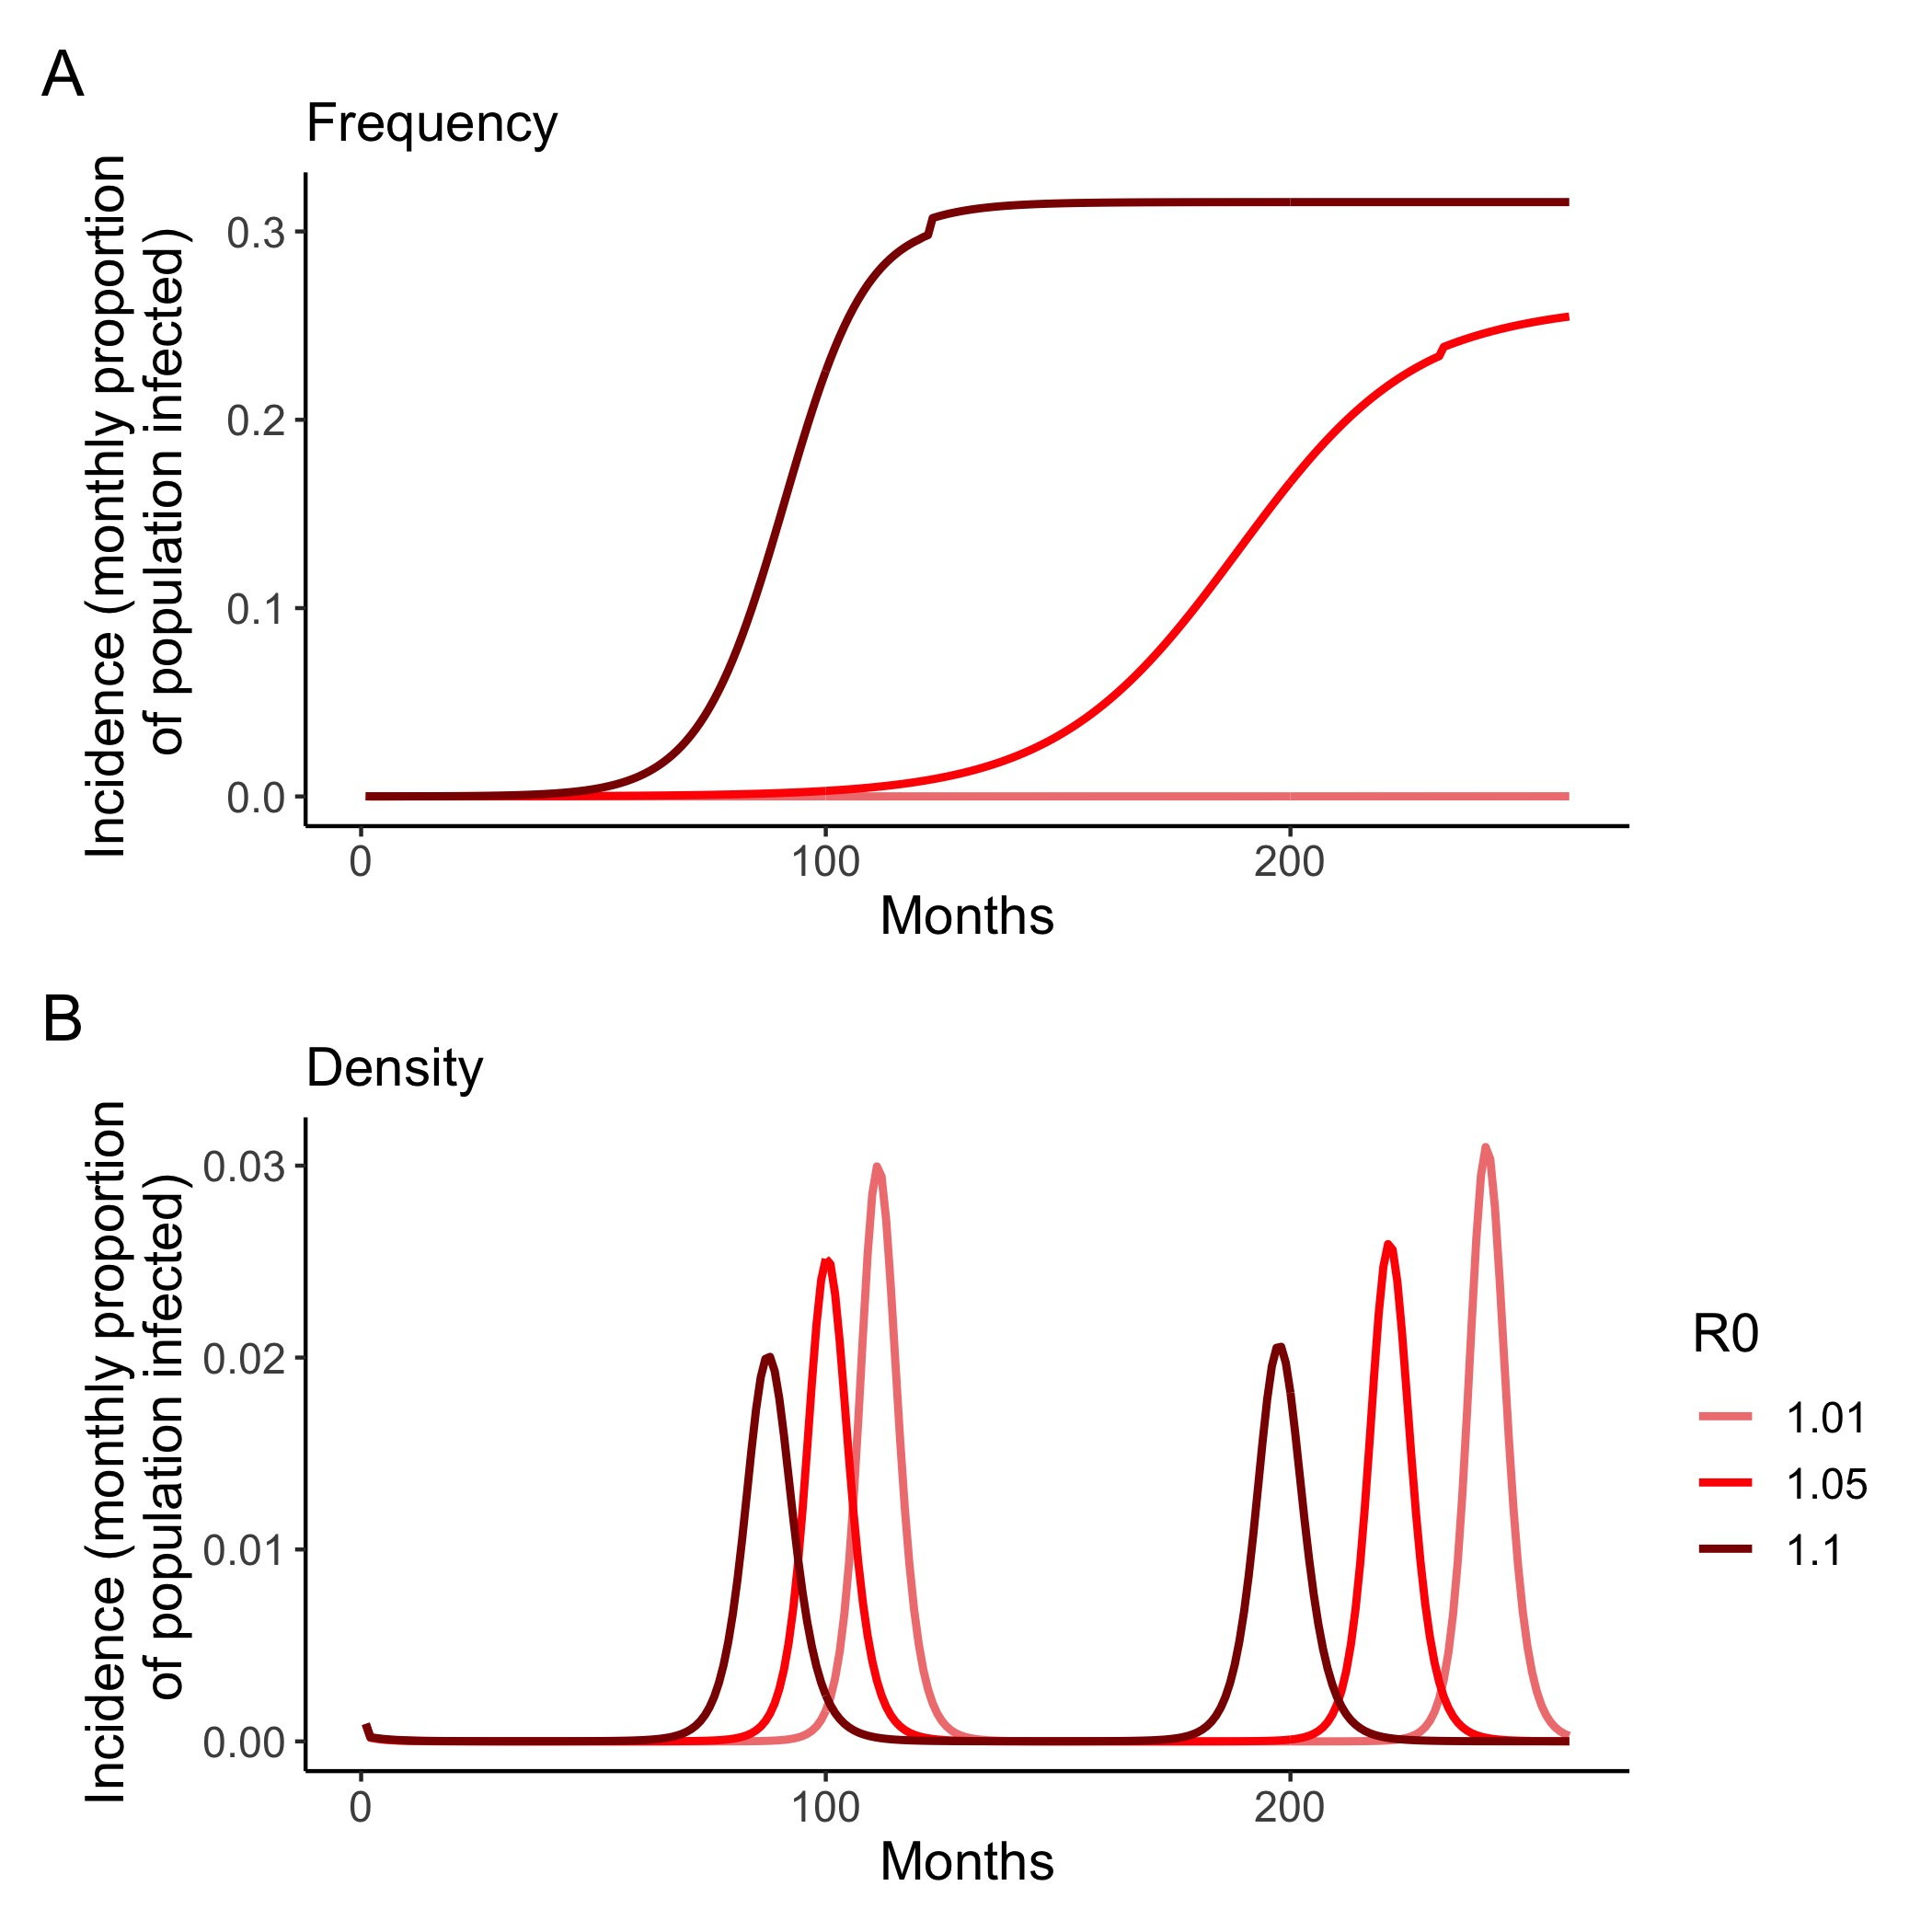
\includegraphics[width=0.8\linewidth]{figs/ch3/image4} \caption[Density vs. frequency-dependent transmission.]{Density vs.~frequency-dependent transmission.
Monthly incidence (the proportion of the population
infected, and thus removed (as a result of mortality)) from mass-action
models of rabies with A) frequency and B) density dependent
transmission. Even in low transmission scenarios (R0 = 1.01 - 1.1),
incidence peaks at between 1.5 -- 2.0\% per month for models with
density-dependent transmission and between 0.01 - 30\% for
frequency-dependent transmission, compared with the 1 - 2\% max annual
incidence observed empirically. Demographic and transmission parameters
are listed in Table \ref{tab:ch4-tab1} (mean incubation and infectious periods were
input as annual rates). Frequency-dependent model is a SEI model with
starting dog population of 50,000 and seeded with 2 infectious
individuals. Density-dependent model is adapted from Anderson et al.
1981, with starting population density of 15 dogs per km\textsuperscript{2} , 0.01
infectious dogs per km\textsuperscript{2}, and carrying capacity of 29 dogs per km\textsuperscript{2}.}\label{fig:figS1}
\end{figure}

















\begin{figure}
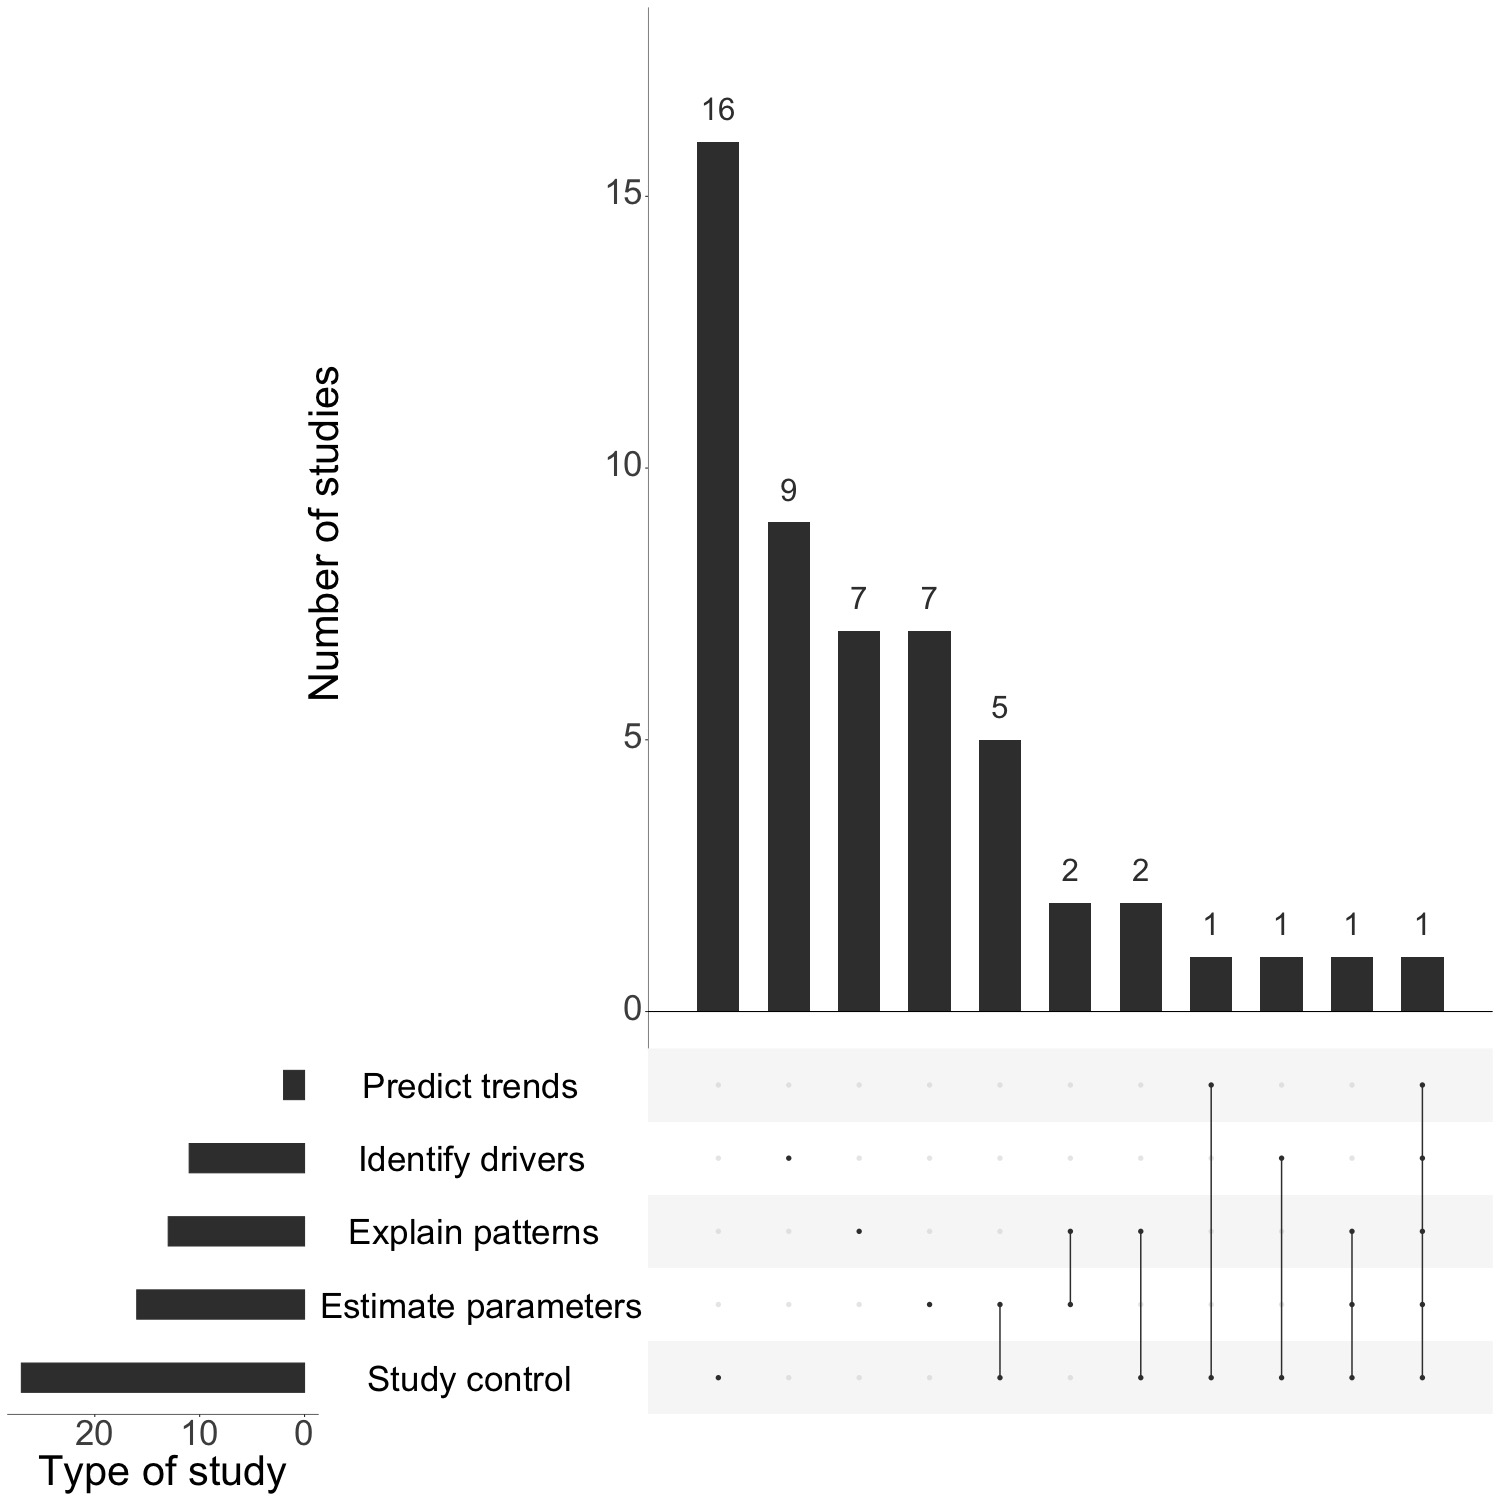
\includegraphics[width=0.8\linewidth]{figs/ch3/image5} \caption[Types of canine rabies modeling studies.]{Types of modeling studies. Categories areadapted from Lloyd-Smith et al.~2009: 1) Predict future trends based on
currently available data and model projections; 2) Study control
measures (using models to estimate/simulate the impacts of control
efforts and compare intervention strategies); 3) Estimate key parameters
such as R\textsubscript{o}, the incubation period, the dispersal kernel; we also
differentiate between studies which 4) Identify drivers of dynamics
(that is look at hypothetical factors which may drive transmission\emph{
}without comparing or fitting to data) and studies which 5) Explain
observed patterns (use models and data to determine likely drivers of
observed patterns).}\label{fig:figS2}
\end{figure}












\hypertarget{spatial-scale-of-control-and-mixing-predicts-dynamics-of-canine-rabies}{%
\chapter{Spatial scale of control and mixing predicts dynamics of canine rabies}\label{spatial-scale-of-control-and-mixing-predicts-dynamics-of-canine-rabies}}

\newpage
\beginmain

\setlength{\parskip}{2em}

\hypertarget{abstract-3}{%
\section*{Abstract}\label{abstract-3}}
\addcontentsline{toc}{section}{Abstract}

Canine rabies is a devastating and preventable disease that causes a high burden of deaths globally each year, particularly in low-and-middle countries where investment in control is limited. Given the mounting evidence that elimination of these deaths is possible, the WHO has set a target to eliminate canine rabies deaths in humans by the year 2030. Mathematical models are a powerful tool to inform these efforts, but to date, efforts to develop robust modeling frameworks for domestic dog populations have been hampered by a lack of data, and inconsistencies between model results and observed dynamics. Here, we use a spatially rich, long-term dataset on canine rabies cases in the Serengeti District in Tanzania. Using parallel data on vaccination campaigns and the underlying spatial distribution of the domestic dog population, we use a simulation-based inference approach to fit our models to key spatiotemporal features of the data. We find that incorporating both the spatial scale of population mixing and the scale of control are key to recovering observed dynamics. We use these results to explore different vaccination scenarios, and find that high spatial coverage of vaccination campaigns is necessary to prevent outbreaks of canine rabies. Moving forward these results provide practical insights into control strategies and modeling methods, as well as shed light on key processes driving rabies transmission.

\hypertarget{introduction-4}{%
\section{Introduction}\label{introduction-4}}

Rabies is a devastating and fatal disease that causes an estimated 60,000 human deaths annually across the globe \protect\hyperlink{ref-hampson2015}{{[}18{]}}. However, these deaths are preventable through post-exposure vaccination, which is highly effective at preventing death if administered promptly after exposure, and through vaccination of domestic dogs, which with sufficient coverage can interrupt transmission and lead to elimination \protect\hyperlink{ref-lankester2014}{{[}29{]}}. The World Health Organization and its partners have set a goal to eliminate deaths due to canine-mediated rabies by the year 2030 through a combination of these interventions \protect\hyperlink{ref-abela-ridder2016}{{[}19{]}}.

While there is a rich history of modeling wildlife rabies transmission dynamics, the body of work for canine rabies is much sparser. Critically, traditional models of wildlife rabies dynamics fail to capture patterns of incidence observed in endemic and epidemic scenarios for dog rabies (i.e.~low and persistent endemic incidence without substantial depletion of the host population). However, we have a strong understanding of rabies epidemiology and biology: transmission does not appear to scale with dog densities evidenced by consistent \(R_{0}\) estimates between 1 - 2 across a range of settings; the infectious period is short and infection is almost invariably fatal; and key epidemiological parameters such as the dispersal kernel and the incubation period are characterized by a long tail. While R0 estimates are consistent and low, there is considerable heterogeneity in transmission with many infectious dogs biting no others, while some may bite upwards of 20 - 50 others \protect\hyperlink{ref-rajeev2020modeling}{{[}26{]}}.

While the epidemiological backbone of rabies is clear, there is little data on disease dynamics in domestic dogs with which to confront models \protect\hyperlink{ref-scott2017}{{[}30{]}}. In fact, most modeling studies of canine rabies are simulation based, with few studies actually fitting models to data \protect\hyperlink{ref-rajeev2020modeling}{{[}26{]}}. This is largely due to poor surveillance (likely substantially less than 5\% of cases are detected annually in endemic settings\protect\hyperlink{ref-townsend2013a}{{[}31{]}}), but given the epidemiological features of rabies combined with low detection rates, inference can be challenging. Rabies outbreaks are highly stochastic and likely driven by heterogeneities and rare events. Therefore traditional inference methods based on times series data alone are likely to fail when confronted with the noisy reality of rabies data.

Recent advances in simulation based inference have facilitated fitting to data from highly stochastic and noisy systems using more complex models with analytically intractable likelihoods \protect\hyperlink{ref-funk2020}{{[}16{]}}, \protect\hyperlink{ref-hazelbag2020}{{[}32{]}}. One such method is Approximate Bayesian Computation, with fits to features of the data rather than each individual observation \protect\hyperlink{ref-hazelbag2020}{{[}32{]}}. These methods are useful tools for model comparison, and present a way forward to assess what level of complexity is needed in models to predict observed dynamics.

Here we use a uniquely comprehensive long-term dataset on canine rabies cases in space and time across the Serengeti District in Tanzania, where ongoing vaccination campaigns have shaped dynamics over the past twenty years. We build on recent work that highlights the role of spatial structure in mixing \protect\hyperlink{ref-Mancyinprep}{{[}28{]}}, simplifying the model, extending it to consider different movement scenarios, and comparing models at the scale of population mixing (\textasciitilde{} 1 km) vs.~at the scale of control (village scale). Coupled with data on vaccination and the spatial distribution of the dog population, we build an individual-based spatially explicit model, and using a simulation-based inference approach, fit it to key spatiotemporal features of the observed data to identify models that best fit our data and generate realistic dynamics in endemic situations. Finally, we simulate vaccination campaigns and control strategies based on our findings to inform control efforts.

\hypertarget{methods-2}{%
\section{Methods}\label{methods-2}}

\hypertarget{study-area}{%
\subsection{Study area}\label{study-area}}

The Serengeti District in Tanzania is approximately 2000 km\textsuperscript{2} in area and is comprised of of multi-ethnic agropastoralist communities (estimated human population of \ensuremath{2.49\times 10^{5}} at the time of the last census in 2012) with high dog ownership (estimated human-to-dog ratios ranging from 3 to 9). Rabies has been endemically circulating in the district, with documented outbreaks reported as early as the 1950s \protect\hyperlink{ref-brunker2015}{{[}25{]}}, and rabies vaccination campaigns have been ongoing in the district since the early 1990s. Through multi-institutional partnerships with the Tanzanian government and vaccine manufacturers, these have expanded into a large scale control program.

Since 2002, a long-term contact tracing study of canine rabies and domestic dogs has been ongoing in the district \protect\hyperlink{ref-Hampson2009}{{[}33{]}}, with data collected on clinical and laboratory diagnosed cases of animal rabies, as well as vaccination and dog ownership data. Here we use three key datasets from this study system:

\begin{enumerate}
\def\labelenumi{\arabic{enumi})}
\item
  Case histories of clinical and laboratory diagnosed dog rabies cases between 2002 - 2020 (N = 3179 observations with and approximate date of symptom onset and GPS location (\ref{fig:data}A and B).
\item
  \begin{enumerate}
  \def\labelenumii{\arabic{enumii})}
  \setcounter{enumii}{2}
  \tightlist
  \item
    A full household and dog census of the district conducted between 2009 - 2014, with the spatial location of households, the number of people and of adult dogs and puppies in each household, and their vaccination status (\ref{fig:data}C).
  \end{enumerate}
\item
  A full household and dog census of the district conducted between 2009 - 2014, with the spatial location of households, the number of adult dogs and puppies in each household, the number of individuals in these households, and dog vaccination status (\ref{fig:data}D).
\end{enumerate}

We also used census data on human population sizes from the 2002 and 2012 national census in Tanzania to estimate population growth over the district. Village (i.e.~administrative level 3) boundaries for the district were constructed using the distribution of household locations belonging to each village from the dog census data (\ref{fig:data}D, \protect\hyperlink{ref-Mancyinprep}{{[}28{]}}).

\begin{figure}
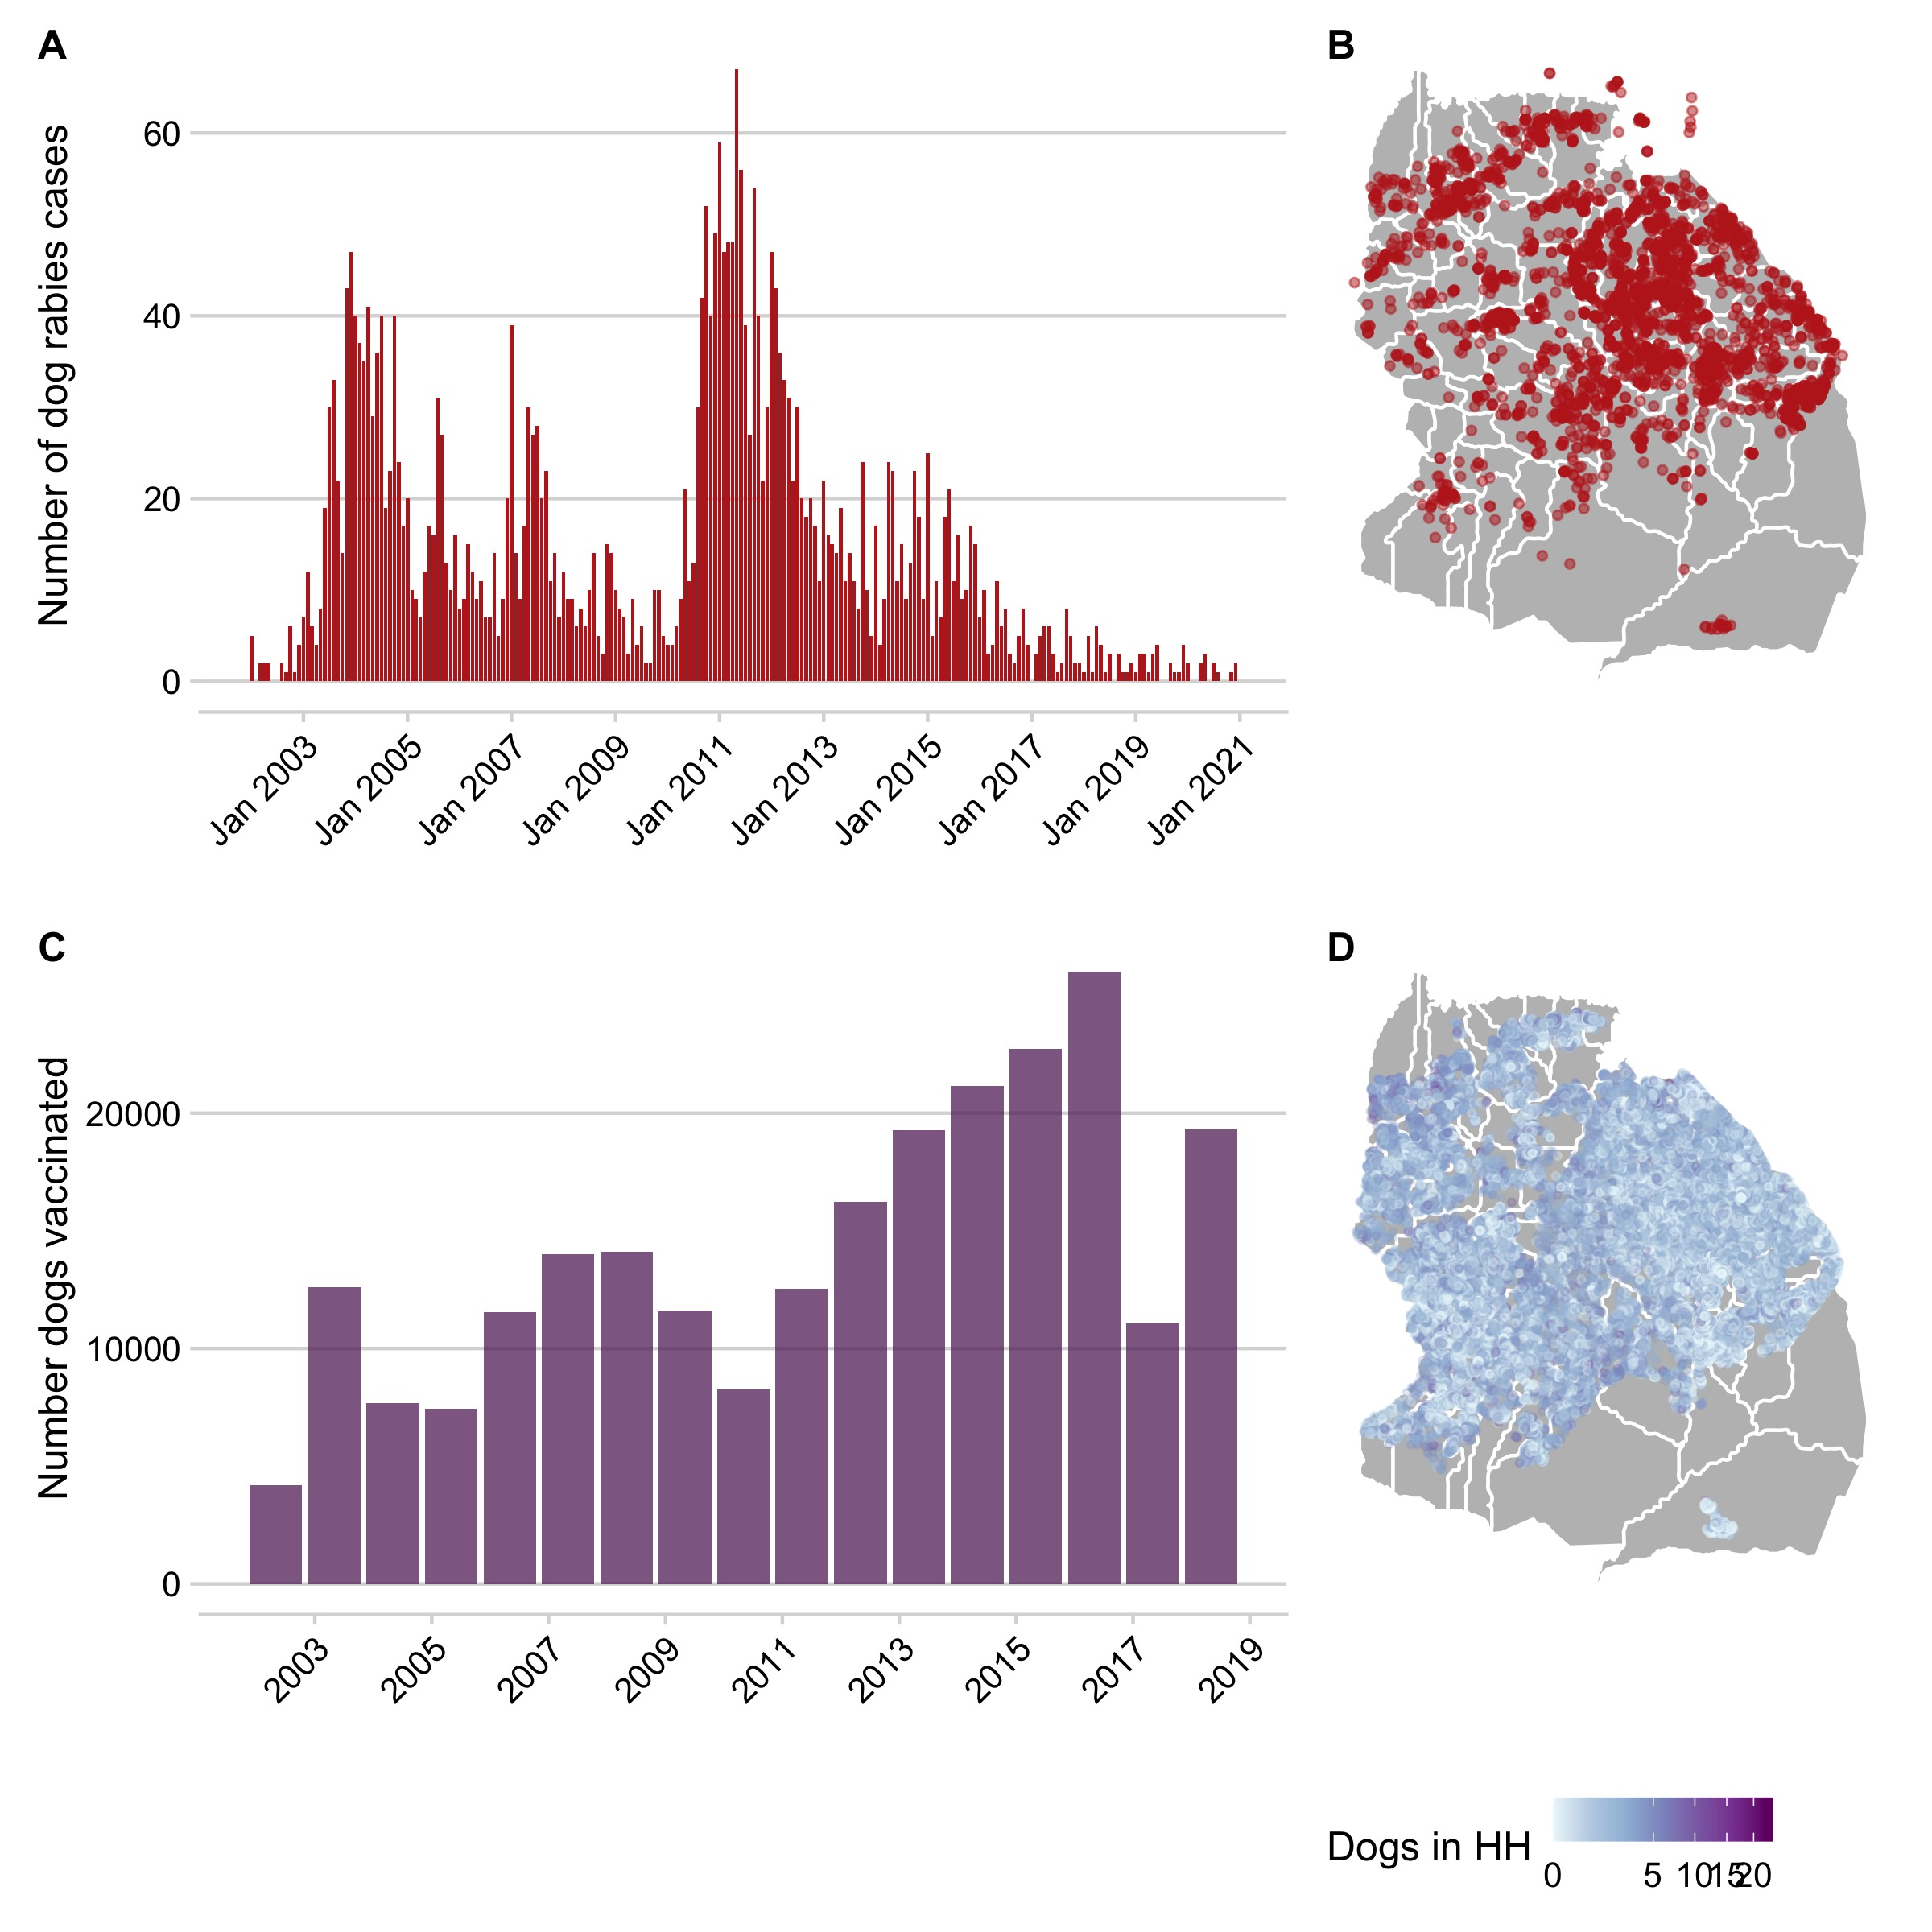
\includegraphics[width=0.9\linewidth]{/Users/mrajeev/Documents/Projects/dynamicSD/analysis/figs/fig_data} \caption[Datasets on rabies cases, vaccination, and distribution of the dog population used in the analyses.]{Datasets used in the analyses. A) Shows the time series of monthly rabies cases in domestic dogs and B) shows their spatial distribution across the district. C) The annual number of dogs vaccinated each year during mass campaigns. D) The location of household census data with colors showing the number of dogs owned per household. Polygons delineate village boundaries in the district.}\label{fig:data}
\end{figure}



\hypertarget{a-spatially-explicit-individual-based-model-of-rabies-transmission}{%
\subsection{A spatially-explicit, individual-based model of rabies transmission}\label{a-spatially-explicit-individual-based-model-of-rabies-transmission}}

We developed a discrete-time, individual-based, Susceptible-Exposed-Infectious-Vaccinated transmission model to simulate rabies dynamics in the domestic dog population. Transmission occurs at the individual level with secondary cases drawn from a right censored negative binomial distribution with mean \(R_{0}\) and dispersion parameter \(k\) (to capture heterogeneity, but constrained so that secondary cases from a single individual do not exceed 100 cases, a realistic range of transmission potential). Movement of infectious individuals occurs in continuous space, with distances either drawn as a dispersal distance (log normal distribution, i.e.~case movements are all drawn in reference to the progenitor location) or as a random walk with a Weibull step length distribution, (i.e.~case movements are sequential). The timing of when a dog becomes infectious after exposure is drawn from a lognormal serial interval distribution (the infectious period + the incubation period). Previous work has shown the importance of introductions of rabies cases from outside the district in maintaining transmission within the district \protect\hyperlink{ref-Mancyinprep}{{[}28{]}}. We use two approaches to simulate introductions:

\begin{enumerate}
\def\labelenumi{\arabic{enumi})}
\tightlist
\item
  Using inferred locations of introductions from transmission tree reconstruction between 2002 - 2015 to explicitly seed transmission chains
\item
  Drawing the number of weekly introductions as a poisson distributed variable (\(\iota\)) and randomly seeding them in space
\end{enumerate}

Demographic processes occur sequentially and are aggregated to the spatial scale being modeled: new dogs are born according to village level birth rates; dogs die at a fixed rate across the district, and finally vaccination occurs. Vaccinations are allocated from the village level to the spatial scale being modeled, allocated by population size in a given location, and we assume that surviving vaccinated dogs are re-vaccinated in subsequent campaigns, giving a conservative estimate of vaccination. To get initial dog population sizes in each location, we estimate human:dog ratios from the dog census data, and apply them to human population estimates from national census data at the start of our simulation period (2002). We allocate them spatially according to the distribution of households and dogs from the census data. To get village level growth rates, we estimate human population growth between 2002 - 2012 from the national census data at the village level and assume that dog populations grow at that same rate (and assume a fixed death rate, Table \ref{tab:tbinputs} \protect\hyperlink{ref-czupryna2016}{{[}34{]}}). We do not apply demographic transitions to exposed or infectious individuals (i.e.~they only move out of their classes when moving from exposed to infectious or infectious to removed).

We use a weekly time step to aggregate both demographic and transmission events (i.e.~infectious dogs in location x at week t all compete for the same contacts) and explore different scales of spatial mixing: at an 1 km\textsuperscript{2} resolution and at the village scale (in UTM Zone 36S such that distances between grid cells are as close to 1 km as possible). Table \ref{tab:tbinputs} lists all parameters and their sources. In addition to comparing mixing at the village and 1 km scales, we also explore how further constraining movement of rabid dogs impacts model inference. At the baseline, we do not constrain movements of rabid dogs: that is rabid dog movements to locations outside of the district or to inhabited patches will result in a failed transmission event. We compare this baseline (which we refer to hereafter as the no limits model) with a model that restrict movements to only inhabited patches (i.e.~populated patches at the beginning of the simulation, the patch limits model), and finally a model that restricts movement to both uninhabited patches and to the district (the full limits model). For the constrained models, we do not resample individual movements that fail as this could potentially skew the underlying parameter distance distribution (for example, if resampling happens often enough, this can shift both the average and skew of the distribution). Instead, for each movement we draw distances, find grid cells within that distance, and sample movement to valid locations given the model constraints. We assume that infection is completely fatal, and infectious individuals are removed at the end of the weekly timestep during which they became infectious. Finally, to account for imperfect case detection we use a monthly beta binomial detection probability (Table \ref{tab:tbinputs}).

\begin{table}

\caption{\label{tab:tbinputs}Table of parameter inputs and sources.}
\centering
\begin{tabu} to \linewidth {>{\raggedright\arraybackslash}p{10em}>{\raggedright}X>{\raggedright}X}
\toprule
Input (units) & Distribution & Source\\
\midrule
Secondary case distribution (number of dogs) & Right censored negative binomial distribution with mean = $R_{0}$ and dispersion parameter $k$ & $R_{0}$ and $k$ are estimated, prior centered around estimates from \protect\hyperlink{ref-Hampson2009}{{[}33{]}}\\
Weekly rate of introductions & Poisson distribution & Estimated\\
Serial interval distribution (days) & Lognormal distribution with mean = 2.95, and sd = 0.86, for a mean interval of approximately 27 days & \protect\hyperlink{ref-Mancyinprep}{{[}28{]}}\\
Dispersal kernel (meters) & Lognormal distribution with mean = 5.58, and sd = 1.79, for a mean dispersal length of approximately 1483 meters & \protect\hyperlink{ref-Mancyinprep}{{[}28{]}}\\
Step length distribution (meters) & Convolved Weibull distribution with shape = 1.12, and scale = 491.1, for a mean step length of approximately 428.35 meters & \protect\hyperlink{ref-Mancyinprep}{{[}28{]}}\\
\addlinespace
Detection probability (monthly) & Beta binomial distribution with $\beta$ = 8.9, $\alpha$ = 80.1, for a mean monthly detection probability of approximately 0.9 & \protect\hyperlink{ref-Mancyinprep}{{[}28{]}}\\
Annual death rate (dogs/yr) & 1/25.8 yrs & \protect\hyperlink{ref-czupryna2016}{{[}34{]}}\\
Rate of waning vaccine immunity (dogs/yr) & 1/3 yrs & \protect\hyperlink{ref-Hampson2009}{{[}33{]}}\\
\bottomrule
\end{tabu}
\end{table}







\hypertarget{model-selection-parameter-estimation}{%
\subsection{Model selection \& parameter estimation}\label{model-selection-parameter-estimation}}

We use Random Forest Approximate Bayesian Computation (RF-ABC) implemented in the R package \texttt{abcrf} \protect\hyperlink{ref-pudlo2015}{{[}35{]}}, \protect\hyperlink{ref-raynal2018}{{[}36{]}} to perform model selection and parameter inference. We estimate three parameters: \(R_{0}\) (the mean of the secondary case distribution), \(k\) (the dispersion parameter of the secondary case distribution), and \(\iota\) (the mean weekly number of introductions of rabies cases from outside of the district). We use strong priors based on previous analyses of part of this dataset (Table \ref{tab:tbinputs})\protect\hyperlink{ref-Hampson2009}{{[}33{]}}. RF-ABC can be used to evaluate both models and potential summary statistics (i.e.~key features of the data that the model should capture). Table \ref{tab:tbsstats} lists the candidate summary statistics we used for model selection and parameter estimation, encompassing temporal, spatial, and spatiotemporal metrics of the data. RF-ABC ranks each of these parameters by their importance (i.e.~Gini importance, specifically how frequently a variable is used for node classification and broadly a relative measure of the discriminative value a statistic has for the classification problem) in predicting a given parameter or in differentiating models. For both model selection and parameter estimation, we generate N = 1e5 simulated sets of summary statistics. To manage computational resources, we stop any simulations where the host population has declined to greater than 15\% of the starting population, as these simulations generally lead to extinction of domestic dogs and represent unlikely scenarios. We include these simulations in the dataset, but calculate summary statistics only including the data before the simulation was stopped.

We use the default parameter of 500 trees in the random forest for estimation, and also perform a sensitivity analysis with subsets of the full dataset (subsampling to 75\% of simulated dataset) to assess whether estimates are stable. We use prior error rates (the error rate of model classification on simulated datasets withheld from each of the classification trees, i.e.~out-of-bag simulations) for model selection to assess the stability of model estimates to the number of simulated datasets and the number of trees in the Random Forest \protect\hyperlink{ref-raynal2018}{{[}36{]}}. RF-ABC does not allow for joint parameter estimation, however, we approximate joint posteriors by including parameter sets where all estimated parameters were accepted (i.e.~all values were assigned non-zero weights by the random forest classification). We also tested the ability of models to see recovered known parameter estimates using the model to predict out-of-sample simulated datasets across the parameter priors.

We perform model selection for models across all combinations and estimate their posterior probabilities (i.e.~given our observed data, the proportion of trees in our RF model that predicted a given model). We then simulate from the estimated posterior distributions (N = 1000) and compare this to our observed data. We score simulations using the continuous ranked probability score \protect\hyperlink{ref-jordan2019}{{[}37{]}}, and for each simulation of the monthly time series, we also generate centrality scores (i.e.~how representative is a given simulation of the ensemble, \protect\hyperlink{ref-juul2020}{{[}38{]}}) and also the root mean squared error (RMSE) against the observed monthly cases. We also simulate an endemic scenario with no vaccination to see if the models can generate realistic dynamics in this context.

\begin{table}

\caption{\label{tab:tbsstats}Summary statistics used for fitting in Random Forest ABC.}
\centering
\begin{tabu} to \linewidth {>{\raggedright}X>{\raggedright\arraybackslash}p{20em}>{\raggedright}X}
\toprule
Summary statistic & Description & Type\\
\midrule
Max I & Maximum monthly number of cases & Temporal\\
Median I & Median monthly number of cases & Temporal\\
Mean I & Mean monthly number of cases & Temporal\\
Temporal KB & Kullback-Leibler Divergence between observed and simulated distribution of cases temporally & Temporal\\
Spatial KB & Kullback-Leibler Divergence between observed and simulated distribution of cases spatially & Spatial\\
\addlinespace
Mean distance 4 weeks & Mean distance between cases within an 4 week window & Spatiotemporal\\
Mean distance 8 weeks & Mean distance between cases within an 8 week window & Spatiotemporal\\
Mean distance 4 weeks normalized & Mean distances of cases within an 4 week window, normalized by the average distance between all cases & Spatiotemporal\\
Mean distance 8 weeks normalized & Mean distances of cases within an 8 week window, normalized by the average distance between all cases & Spatiotemporal\\
Spatial RMSE & Root mean squared error between the observed vs. simulated density of case locations & Spatial\\
\addlinespace
Spatial loss & Loss value of the absolute difference between observed and simulated cases locations & Spatial\\
Temporal RMSE & Root mean squared error between the observed vs. simulated numbers of monthly cases & Spatial\\
Temporal loss & Loss value of the absolute difference between observed and simulated monthly cases & Temporal\\
Mean distance all cases & Average distance between all cases & Spatial\\
ACF Monthly 1-6 & Autocorrelation values for monthly time series at 1 - 6 month lag & Temporal\\
\addlinespace
ACF Weekly 1-10 & Autocorrelation values for weekly time series at 1 - 10 week lag & Temporal\\
\bottomrule
\end{tabu}
\end{table}

\hypertarget{assessing-simulated-vaccination-campaigns-impact-on-transmission}{%
\subsection{Assessing simulated vaccination campaigns impact on transmission}\label{assessing-simulated-vaccination-campaigns-impact-on-transmission}}

To explore how spatial heterogeneities in vaccination coverage could drive outbreak risk, using the model with the highest posterior probability given our observed data (our `best' model), we simulate across a range of campaign scenarios. We vary both the level of coverage achieved during annual campaigns (campaign coverage), and the proportion of villages which are vaccinated during campaigns (spatial coverage), and use our posterior estimates to simulate transmission dynamics. We simulate these campaigns (N = 100 simulations per combination) with random villages being vaccinated with probability x in each year. We simulate a five year endemic burn-in period, and then simulate annual campaigns over ten years. In the last five year period of the simulation, we calculate summary statistics that capture key metrics of control success such as peak and mean incidence, chain size and length, and weeks where transmission exceeds the 95th\% of the mean incidence of introduced cases only. We also calculate a connectivity based summary statistic at the village level (c) which equals the sum of squares of the component size of the village graph, where villages are connected if they are adjacent and if coverage at that time step exceeds a threshold (the campaign coverage for a given simulation).

\hypertarget{assessing-the-impact-of-additional-interventions-on-transmission-and-outbreak-probabilities.}{%
\subsection{Assessing the impact of additional interventions on transmission and outbreak probabilities.}\label{assessing-the-impact-of-additional-interventions-on-transmission-and-outbreak-probabilities.}}

Using our best model, we explore how additional interventions implemented alongside vaccination campaigns affect outbreak probabilities and transmission. We simulate approximations of two different interventions in combination with the random village campaigns as described above:
1) `Chopping the tail' of the secondary case distribution \protect\hyperlink{ref-Kain2020}{{[}39{]}}, where we decrease the censoring value as vaccination increases, to approximate how enhanced surveillance and isolation/quarantine/removal of rabid dogs can improve control outcomes
2) Reducing introductions as coverage increases, i.e.~approximating coordination of vaccination campaigns across larger spatial scales

Fig \ref{fig:sfig-conn-constraint} shows the simulated reductions in introduction rates and maximum allowed secondary cases given district level coverage..

\hypertarget{data-and-ethics-statement}{%
\subsection{Data and ethics statement}\label{data-and-ethics-statement}}

The data used in these analyses are part of a long term research project in the Serengeti District approved through the University of Glasgow Ethics Board and by the Tanzania Commission for Science and Technology, and National Institute for Medical Research. Anonymized data and code are available at github.com/mrajeev08/dynamicSD (to be archived on Zenodo and made public upon article submission) and the underlying simulation model is available here (github.com/mrajeev08/simrabid). All analyses were done using R \protect\hyperlink{ref-R-program}{{[}40{]}} and the following key packages: abcrf, ranger, data.table, sf, raster, and foreach, \protect\hyperlink{ref-pudlo2015}{{[}35{]}}, \protect\hyperlink{ref-R-sf}{{[}41{]}}--\protect\hyperlink{ref-R-foreach}{{[}45{]}}.

\hypertarget{results-2}{%
\section{Results}\label{results-2}}

\hypertarget{the-scale-of-mixing-and-specification-of-introductions-differentiate-models.}{%
\subsection{The scale of mixing and specification of introductions differentiate models.}\label{the-scale-of-mixing-and-specification-of-introductions-differentiate-models.}}

Model predictions largely varied across two axes: whether introductions were estimated or fixed within the model and the scale of mixing (a 1km\textsuperscript{2} scale vs.~the village scale). The models with kernel based movement and with estimated introduction rates were ranked highest at both scales, Whether movement was constrained (patch limits or full limits model) did not seem to impact model selection (Fig \ref{fig:sfig-mod-ranks}). Summary statistics that best differentiated the models encompassed both spatial and temporal summary statistics, and the linear-discriminant analysis axes (LDAs, decompositions of our summary statistics) generated by the RF ABC model (Fig \ref{fig:mfig-mods}B). These results were robust to subsampling the datasets (Fig \ref{fig:sfig-mod-vimp}) and out-of-bag prior error rates were relatively stable with inclusion of additional trees in the random forest model (Fig \ref{fig:sfig-mod-err}). However, broadly, all the models and priors failed to consistently recapture the major components of the summary statistics (Fig \ref{fig:mfig-mods}A) or clearly differentiate between models within scales (a high prior error rate, with datasets withheld from the classification model misclassified approximately \texttt{r}round(prior\_err\_rate, 2)*100)`\% of the time) (Fig \ref{fig:sfig-mod-ranks}).

\begin{figure}
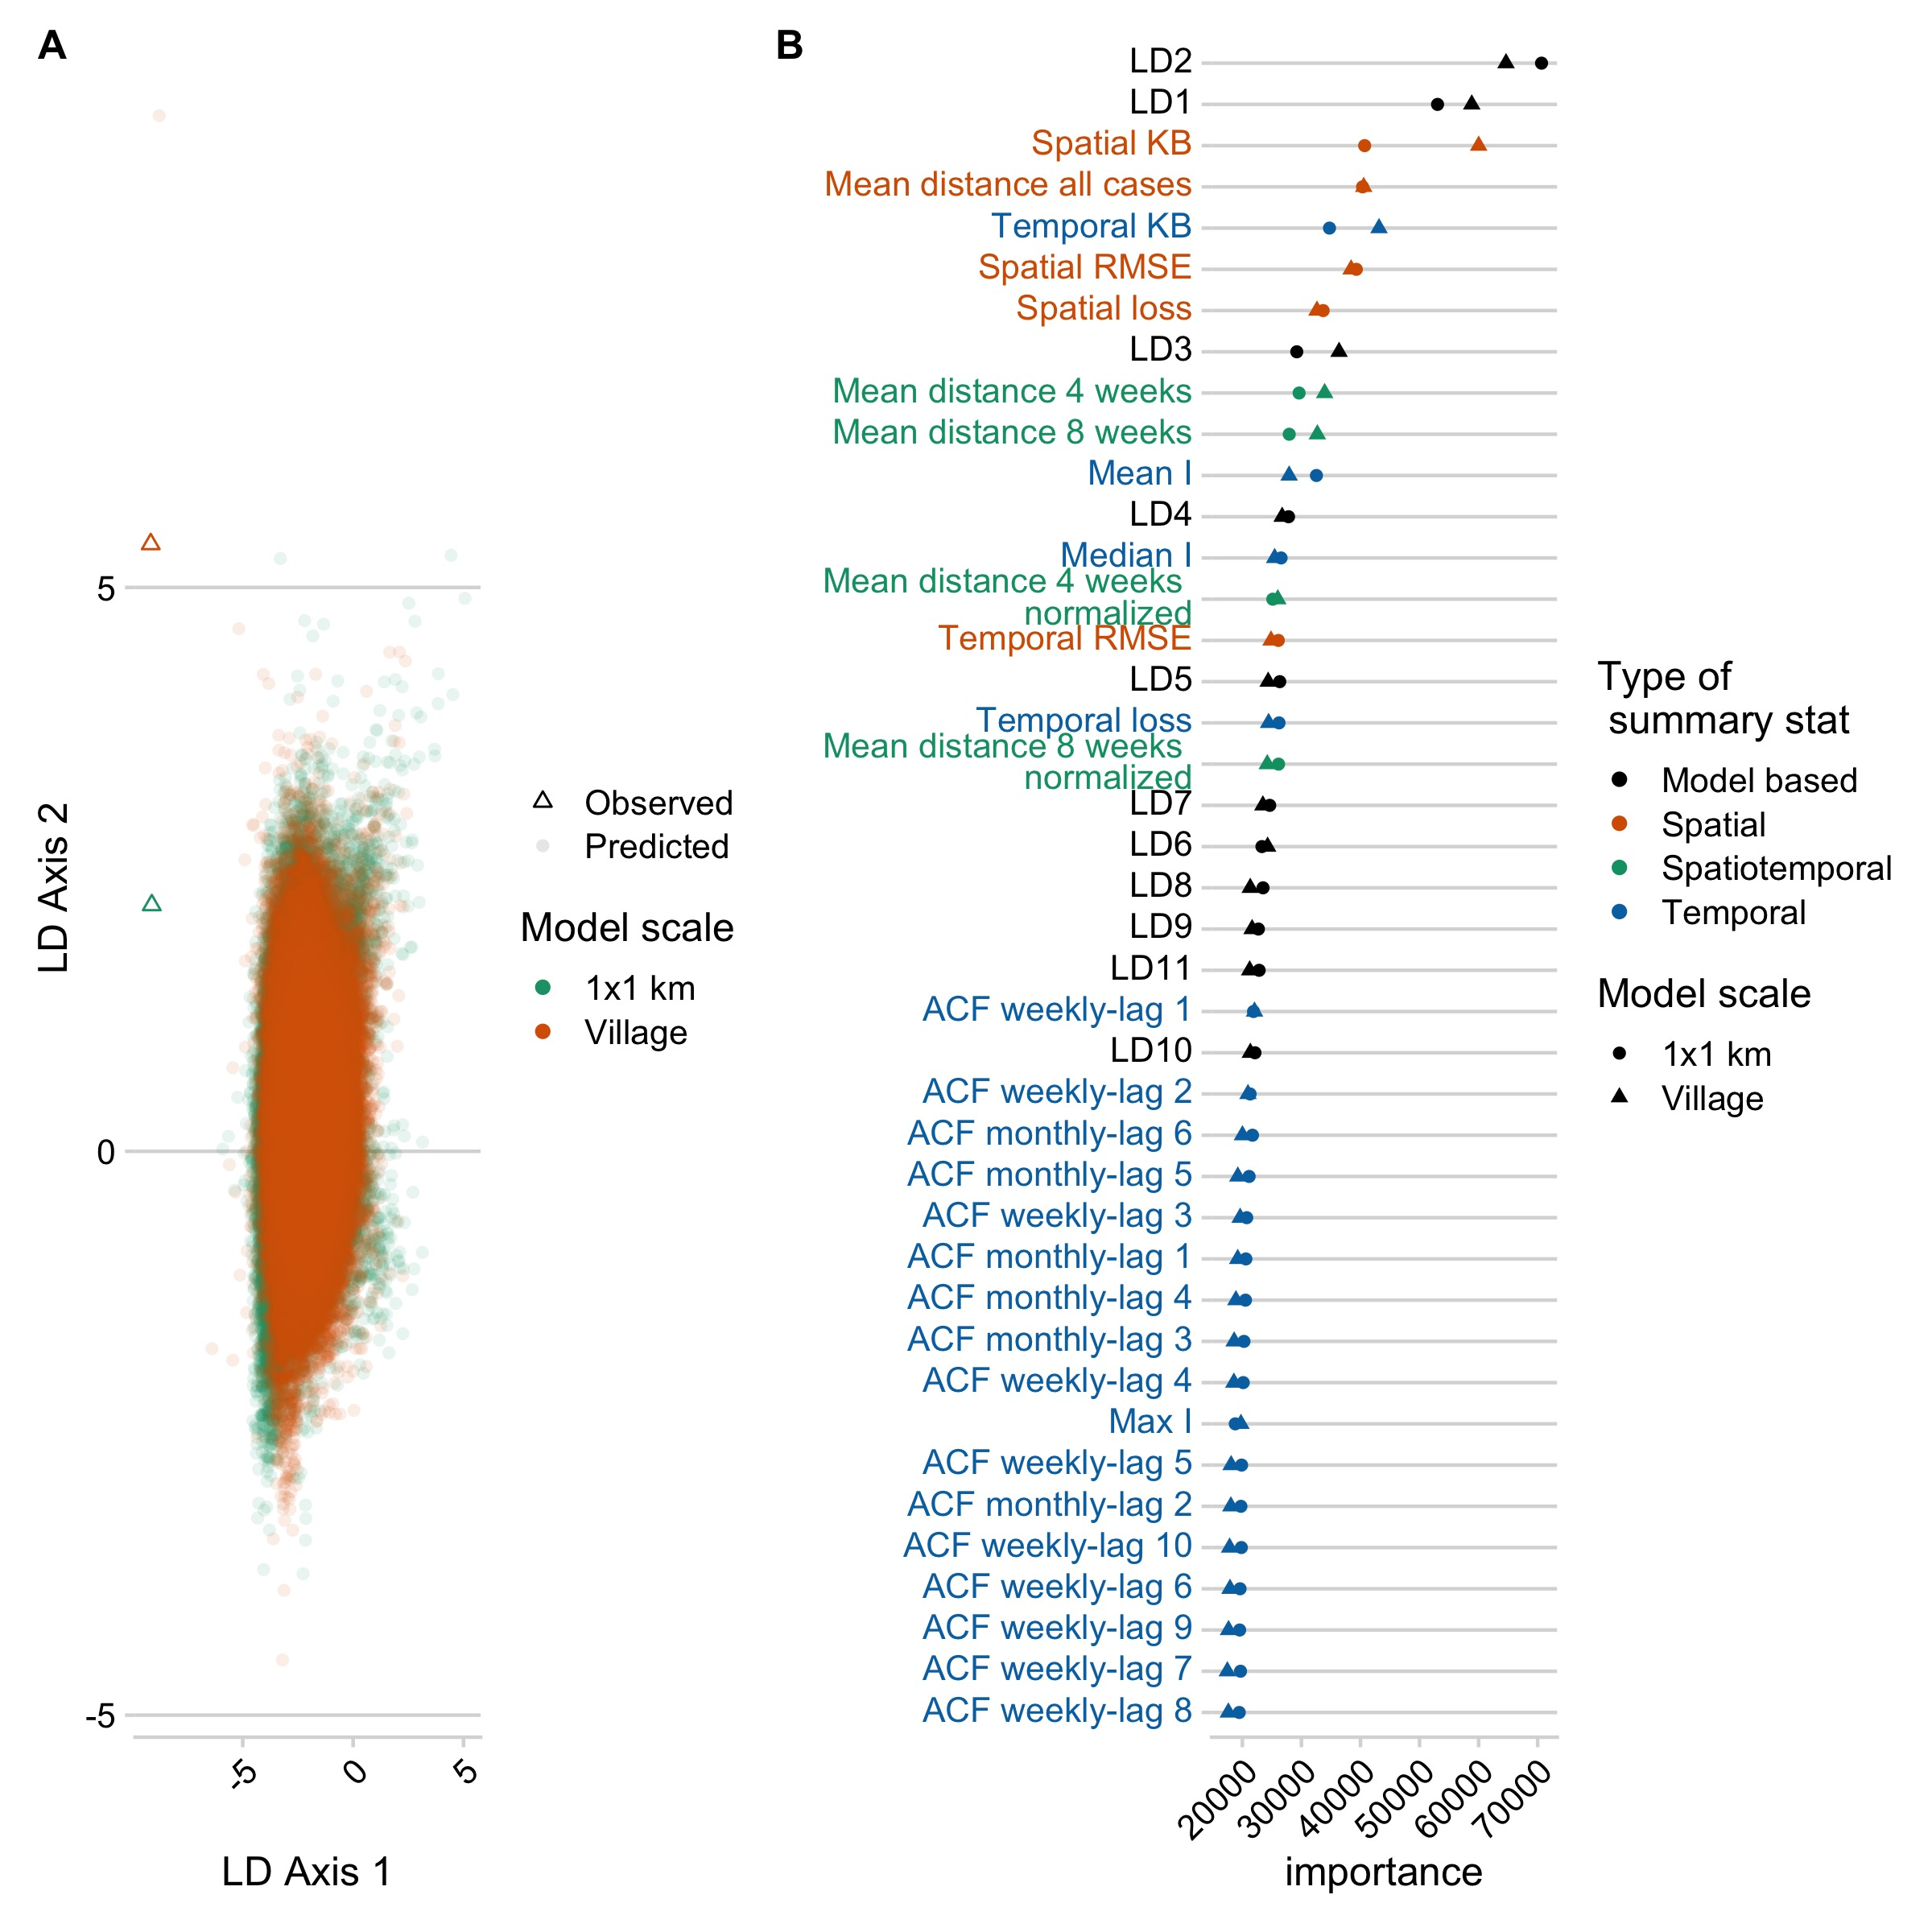
\includegraphics[width=0.9\linewidth]{/Users/mrajeev/Documents/Projects/dynamicSD/analysis/figs/mfig_mod} \caption[Model selection using RF ABC.]{Model selection using RF ABC. A) The two major LDA axes generated by the random forest model for the best model at the village and 1 km scale, with the LDA values predicted for the observed data shown as triangles. B) The importance ranking of each variable in discriminating between models.}\label{fig:mfig-mods}
\end{figure}



\hypertarget{capturing-the-spatial-scale-of-vaccination-and-of-mixing-is-key-to-recovering-the-observed-trajectory-of-rabies-in-the-serengeti-district.}{%
\subsection{Capturing the spatial scale of vaccination and of mixing is key to recovering the observed trajectory of rabies in the Serengeti District.}\label{capturing-the-spatial-scale-of-vaccination-and-of-mixing-is-key-to-recovering-the-observed-trajectory-of-rabies-in-the-serengeti-district.}}

We estimated three parameters: \(R_{0}\), k, and \(\iota\) (for models estimating introductions) using these same models and summary statistics. \(R_{0}\) was best predicted by temporal summary statistics, while k and \(\iota\) were predicted by spatial and spatiotemporal summary statistics (Fig \ref{fig:mfig-posts-vimp}, Fig \ref{fig:sfig-posts-vimp}). Estimates of \(R_{0}\) were consistent and identifiable across the models and robust to subsampling simulations (Fig \ref{fig:sfig-posts-err}), but varied significantly across scales and introduction scenarios (Fig \ref{fig:sfig-posts-jntvsfull}). When comparing posterior estimates for the best models at each scale, \(R_{0}\) estimates were lower in models at the village scale when compared to the 1 km scale (Fig \ref{fig:mfig-posts-best}, Table \ref{tab:tbpars}). Estimates of k and \(\iota\) were more diffuse, and when filtering to parameter sets that had been accepted jointly (i.e.~had non-zero weights for all three parameters), estimates of the introduction rate became sharper, while k became bimodal/skewed (Fig \ref{fig:sfig-posts-jntvsfull}). When we tested the best models at each scale to see whether simulated datasets which were not included in the model fitting could be recovered, we found that \(R_{0}\) and \(\iota\) could be recovered robustly across our prior range, but k was largely unidentifiable (\ref{fig:sfig-par-recov}).

\begin{table}

\caption{\label{tab:tbpars}Priors and independent and joint posterior parameter estimates (mean with 95\% quantiles in parentheses) for the best model at each scale.}
\centering
\begin{tabu} to \linewidth {>{\raggedright\arraybackslash}p{10em}>{\raggedright}X>{\raggedright}X>{\raggedright}X>{\raggedright}X}
\toprule
Scale & Parameter & Prior & Independent posterior & Joint posterior\\
\midrule
1x1 km & $R_{0}$ & 1.13 (0.75 - 1.63) & 1.14 (0.99 - 1.28) & 1.13 (0.97 - 1.27)\\
1x1 km & $k$ & 1.45 (0.48 - 3.44) & 3.04 (0.84 - 7.5) & 4.12 (1.26 - 7.16)\\
1x1 km & $iota$ & 1.13 (0.37 - 2.67) & 1.8 (0.81 - 4.63) & 1.31 (0.85 - 2.14)\\
Village & $R_{0}$ & 1.13 (0.75 - 1.63) & 1.02 (0.91 - 1.13) & 1.03 (0.92 - 1.11)\\
Village & $k$ & 1.46 (0.48 - 3.44) & 3.43 (0.97 - 8.13) & 4.16 (0.78 - 6.28)\\
\addlinespace
Village & $iota$ & 1.13 (0.37 - 2.67) & 2.16 (1.03 - 4.19) & 1.59 (1 - 2.26)\\
\bottomrule
\end{tabu}
\end{table}

\begin{figure}
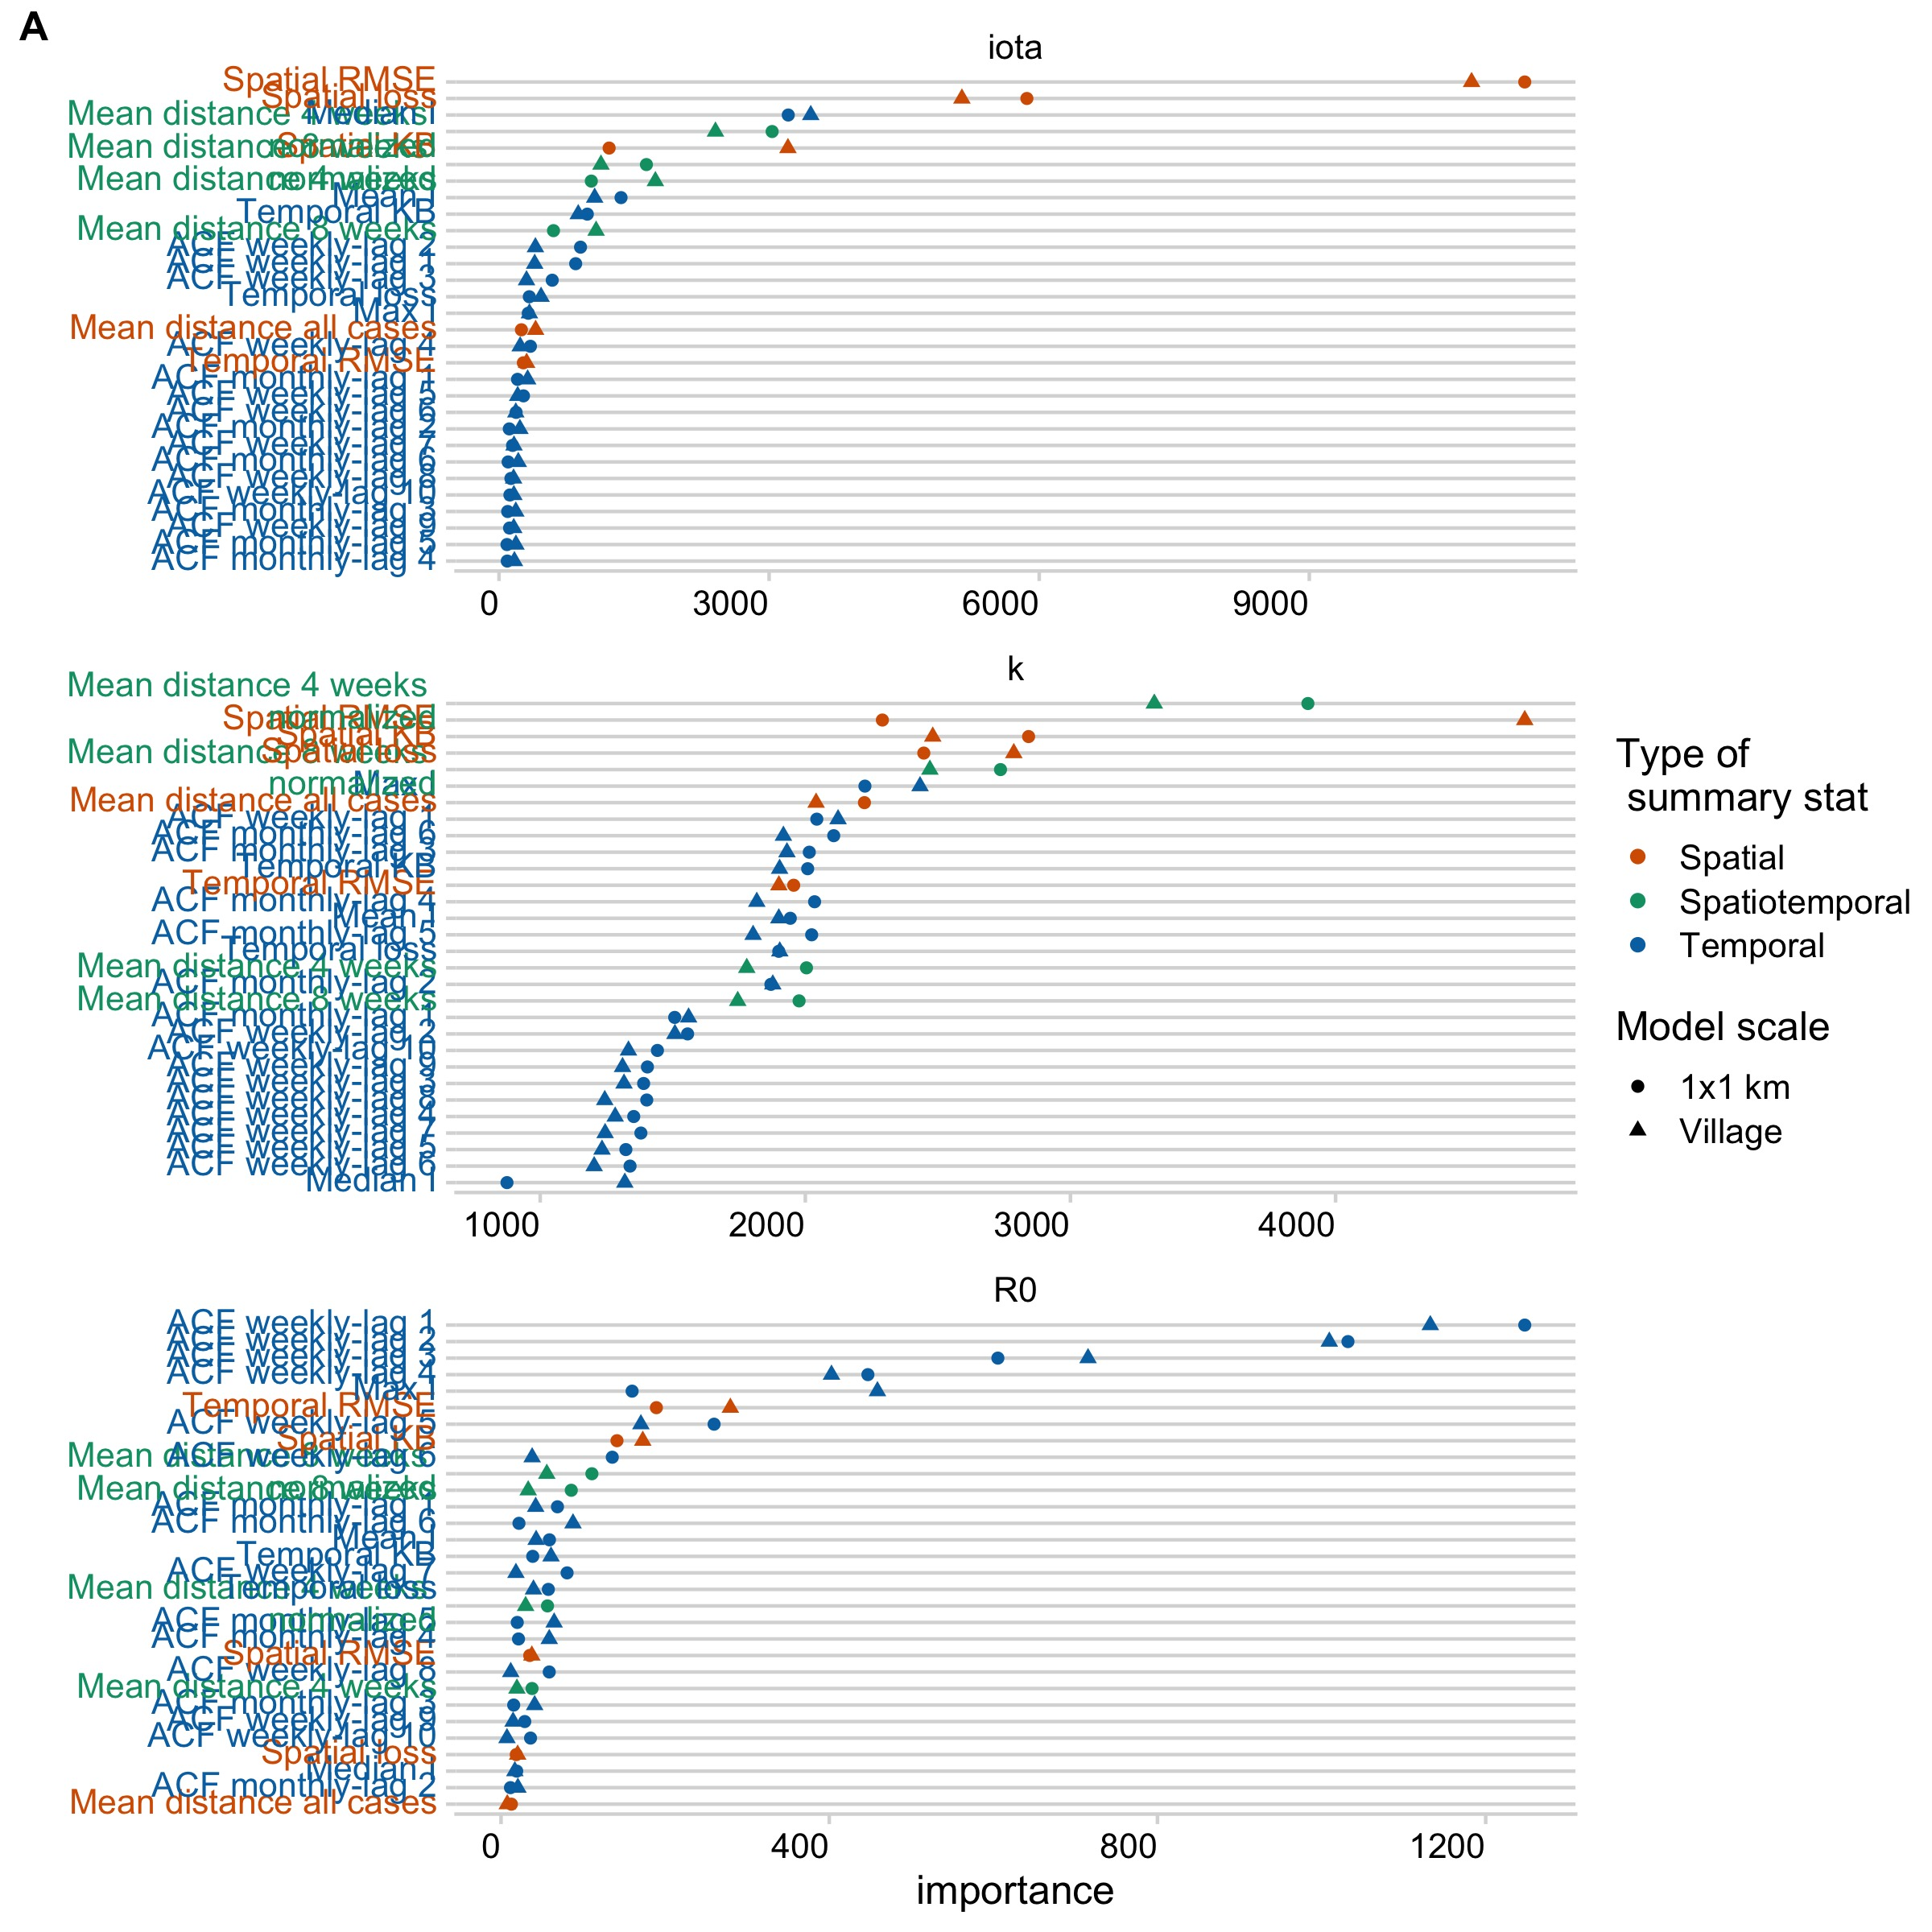
\includegraphics[width=1\linewidth]{/Users/mrajeev/Documents/Projects/dynamicSD/analysis/figs/mfig_posts_vimp} \caption[Ranking of summary statistics for importance in predicting each parameter.]{Ranking of summary statistics for importance in predicting each parameter. Summary statistics are colored by the type of statistic (either spatial, temporal, or spatial temporal). Results are shown for the best fitting model at the village and 1 km scale.}\label{fig:mfig-posts-vimp}
\end{figure}



\begin{figure}
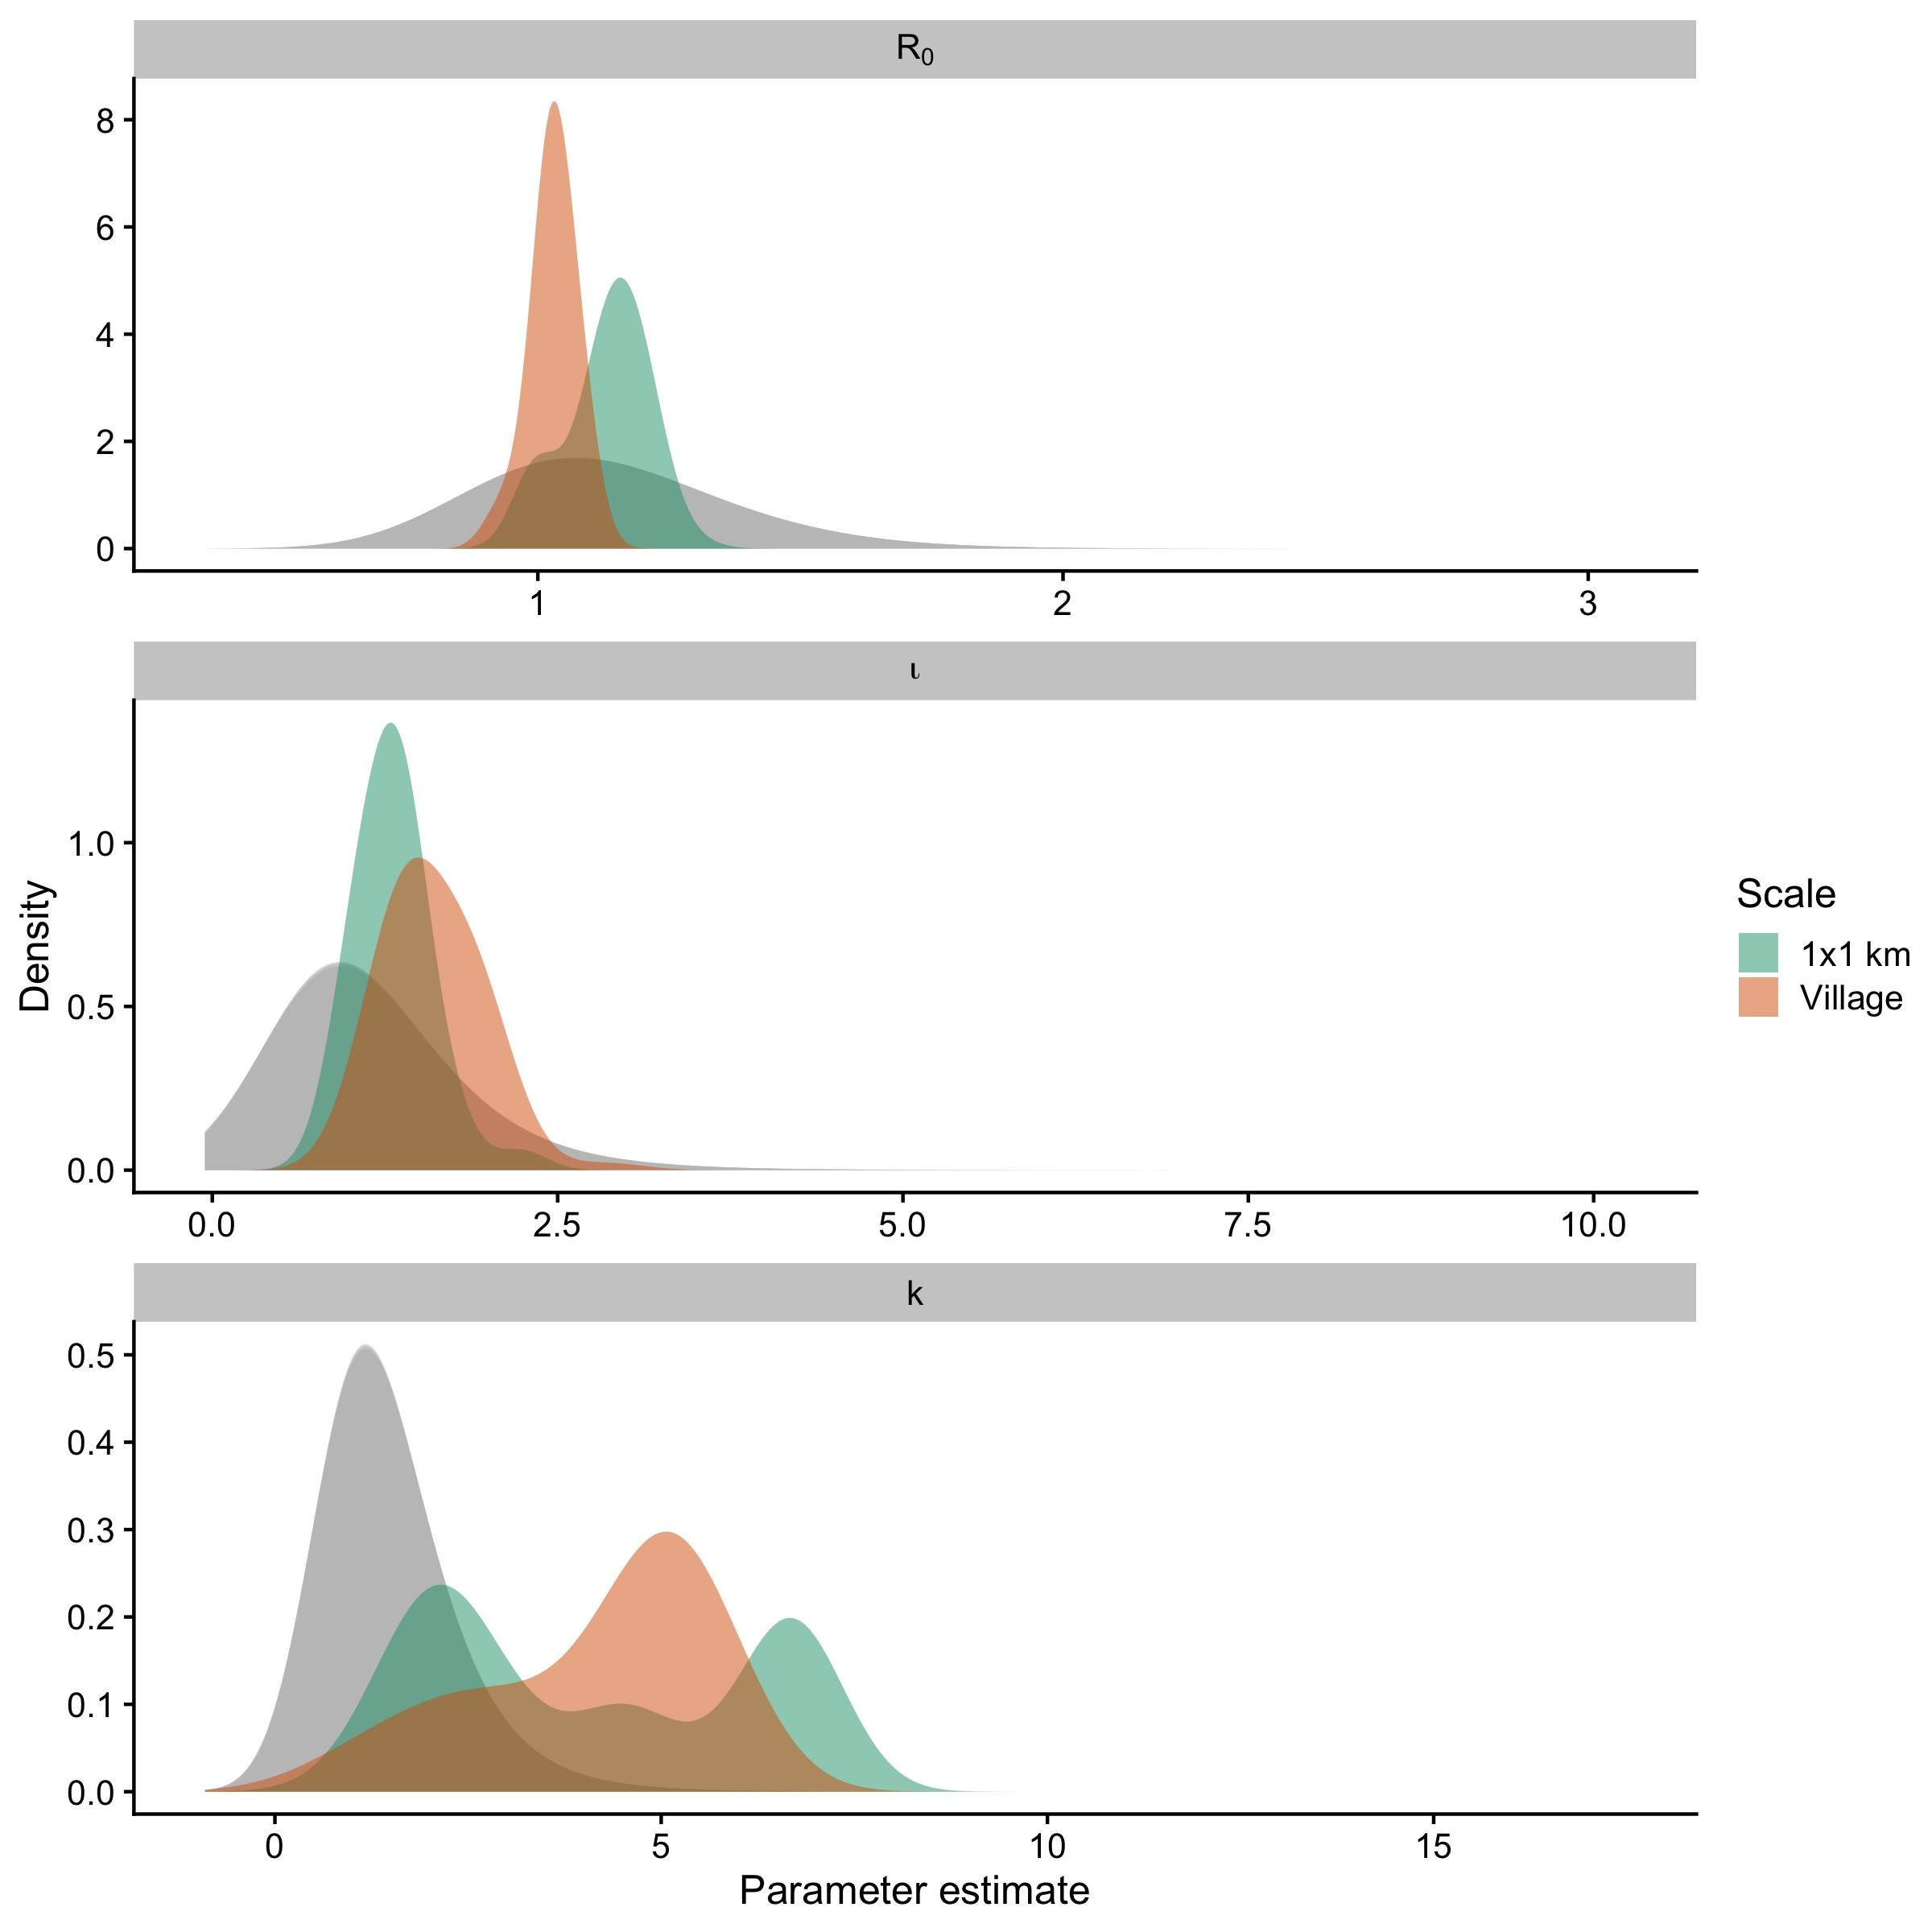
\includegraphics[width=0.9\linewidth]{/Users/mrajeev/Documents/Projects/dynamicSD/analysis/figs/mfig_posts_best} \caption[Independent and joint posterior parameter estimates for the best fitting model across scales.]{Joint posterior estimates compared to prior for the best fitting model at the village and 1 km scale for the three parameters, with prior density in grey.}\label{fig:mfig-posts-best}
\end{figure}



When simulating the data from the posteriors, the models ranked highest by the RF ABC method estimates result in simulations closest to the data observed (Fig \ref{fig:mfig-sims-best}, Fig \ref{fig:sfig-sims-full}). Sampling from the joint parameter sets also improved fits to the data (Fig \ref{fig:sfig-sims-joint}, Fig \ref{fig:sfig-sims-crps}). At both the village and 1 km scale, simulations encompass the trajectory of cases we observed. However, the village scale model fails to capture stable dynamics in an endemic scenario with no vaccination, with transmission resulting in significant declines in the host population, while models at the 1km scale generate stable endemic incidence without depleting the host population (Fig \ref{fig:sfig-sims-endemic}).

\begin{figure}
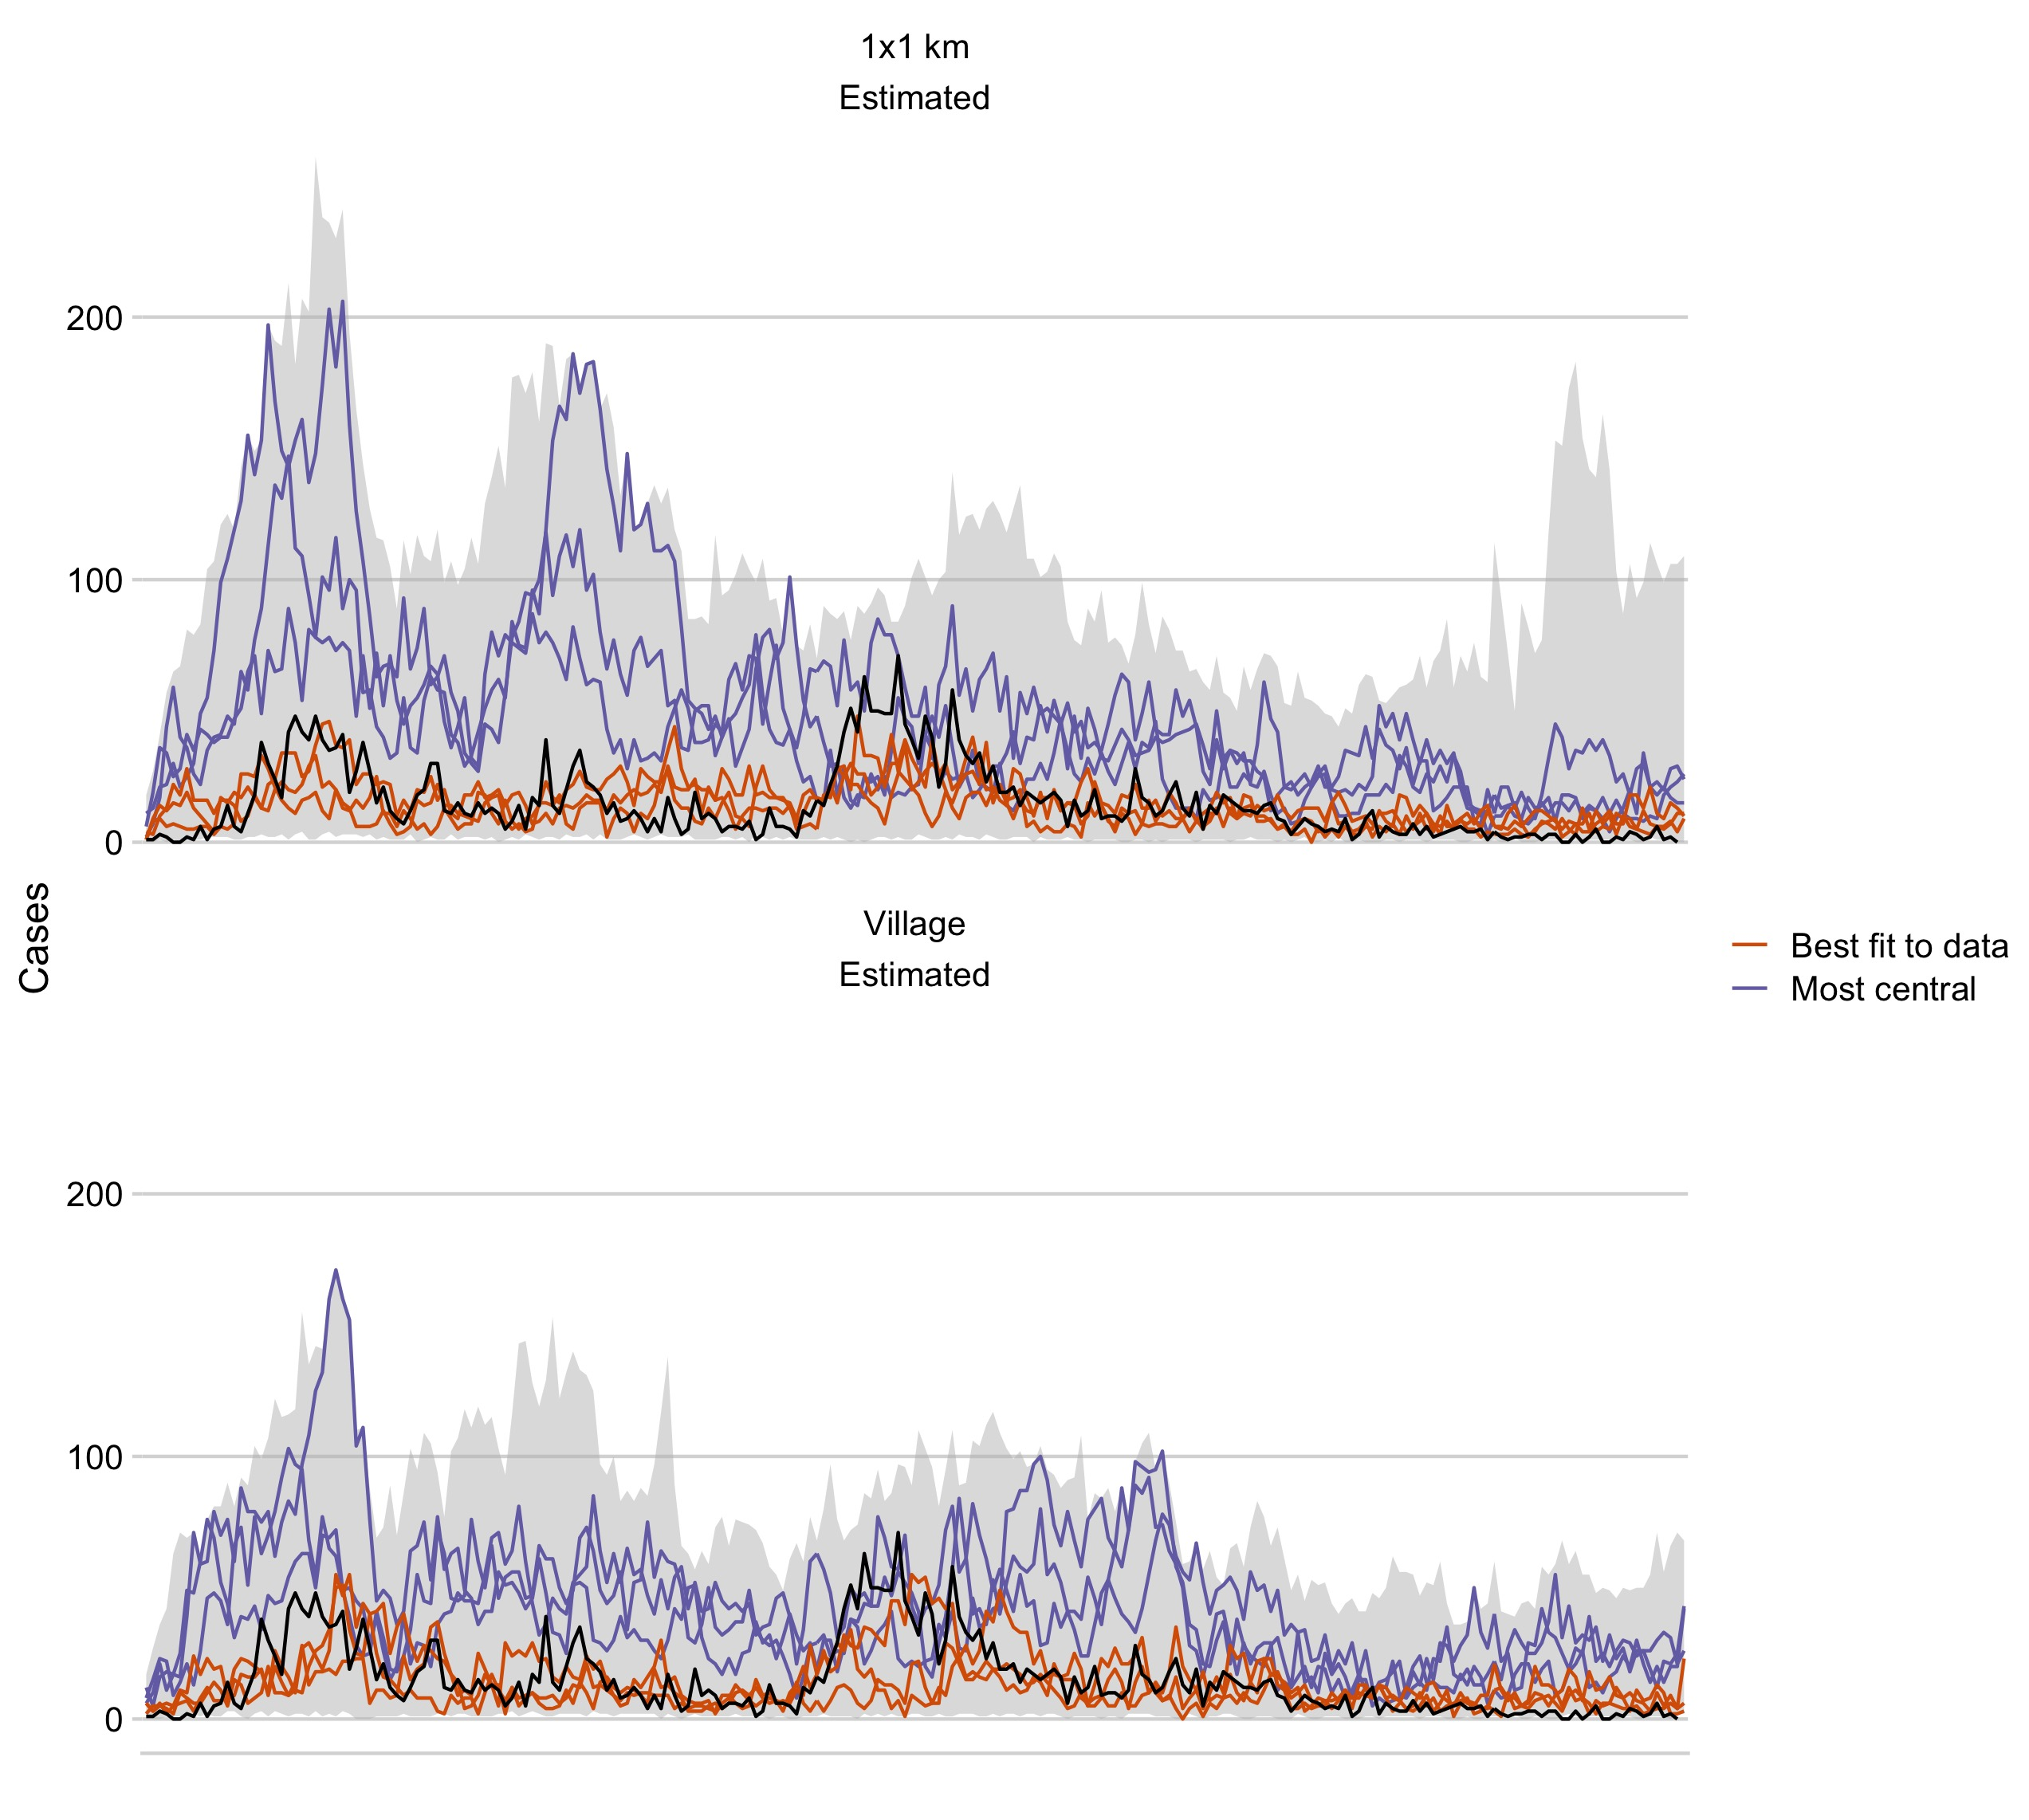
\includegraphics[width=0.9\linewidth]{/Users/mrajeev/Documents/Projects/dynamicSD/analysis/figs/mfig_sims_best} \caption[Simulations from the joint posterior distributions of the best fitting model.]{Simulations from the joint posterior distributions of the best fitting model. The grey envelope shows the range of simulations, and the black line is the time series of observed monthly cases. The orange lines show the top three simulations that best fit the data (lowest RMSE) and the purple lines show the top three simulations that have the highest centrality score.}\label{fig:mfig-sims-best}
\end{figure}



\hypertarget{spatial-coverage-of-vaccination-predicts-control-outcomes-and-interventions-that-target-key-features-of-transmission-improve-these-outcomes.}{%
\subsection{Spatial coverage of vaccination predicts control outcomes and interventions that target key features of transmission improve these outcomes.}\label{spatial-coverage-of-vaccination-predicts-control-outcomes-and-interventions-that-target-key-features-of-transmission-improve-these-outcomes.}}

We find that control outcomes are strongly predicted by both campaign (i.e.~the coverage level achieved by a village campaign) and spatial coverage (the proportion of villages covered by a campaign)(Fig \ref{fig:sfig-base-mets}). We find that campaigns that achieve an annual campaign coverage of 80\% of the population at the village scale and a spatial coverage of 80\% of villages vaccinated are most likely to prevent outbreaks of canine rabies (defined as greater than 4 months with weekly cases greater than the 95\% of the average of the introduced cases) (Fig \ref{fig:mfig-int-comp}). These broadly track with other metrics of control outcomes as well, such as the average peak size and length of transmission chains, and mean and peak incidence (Fig \ref{fig:sfig-base-mets}). In general, both spatial and campaign coverage are more predictive of peak rather than average metrics (Fig \ref{fig:sfig-base-mets}). Connectivity of vaccinated villages varies the most at intermediate spatial coverage, and this metric also broadly predicts control outcomes within a given campaign scenario (Fig \ref{fig:sfig-conn-mets}).

\begin{figure}
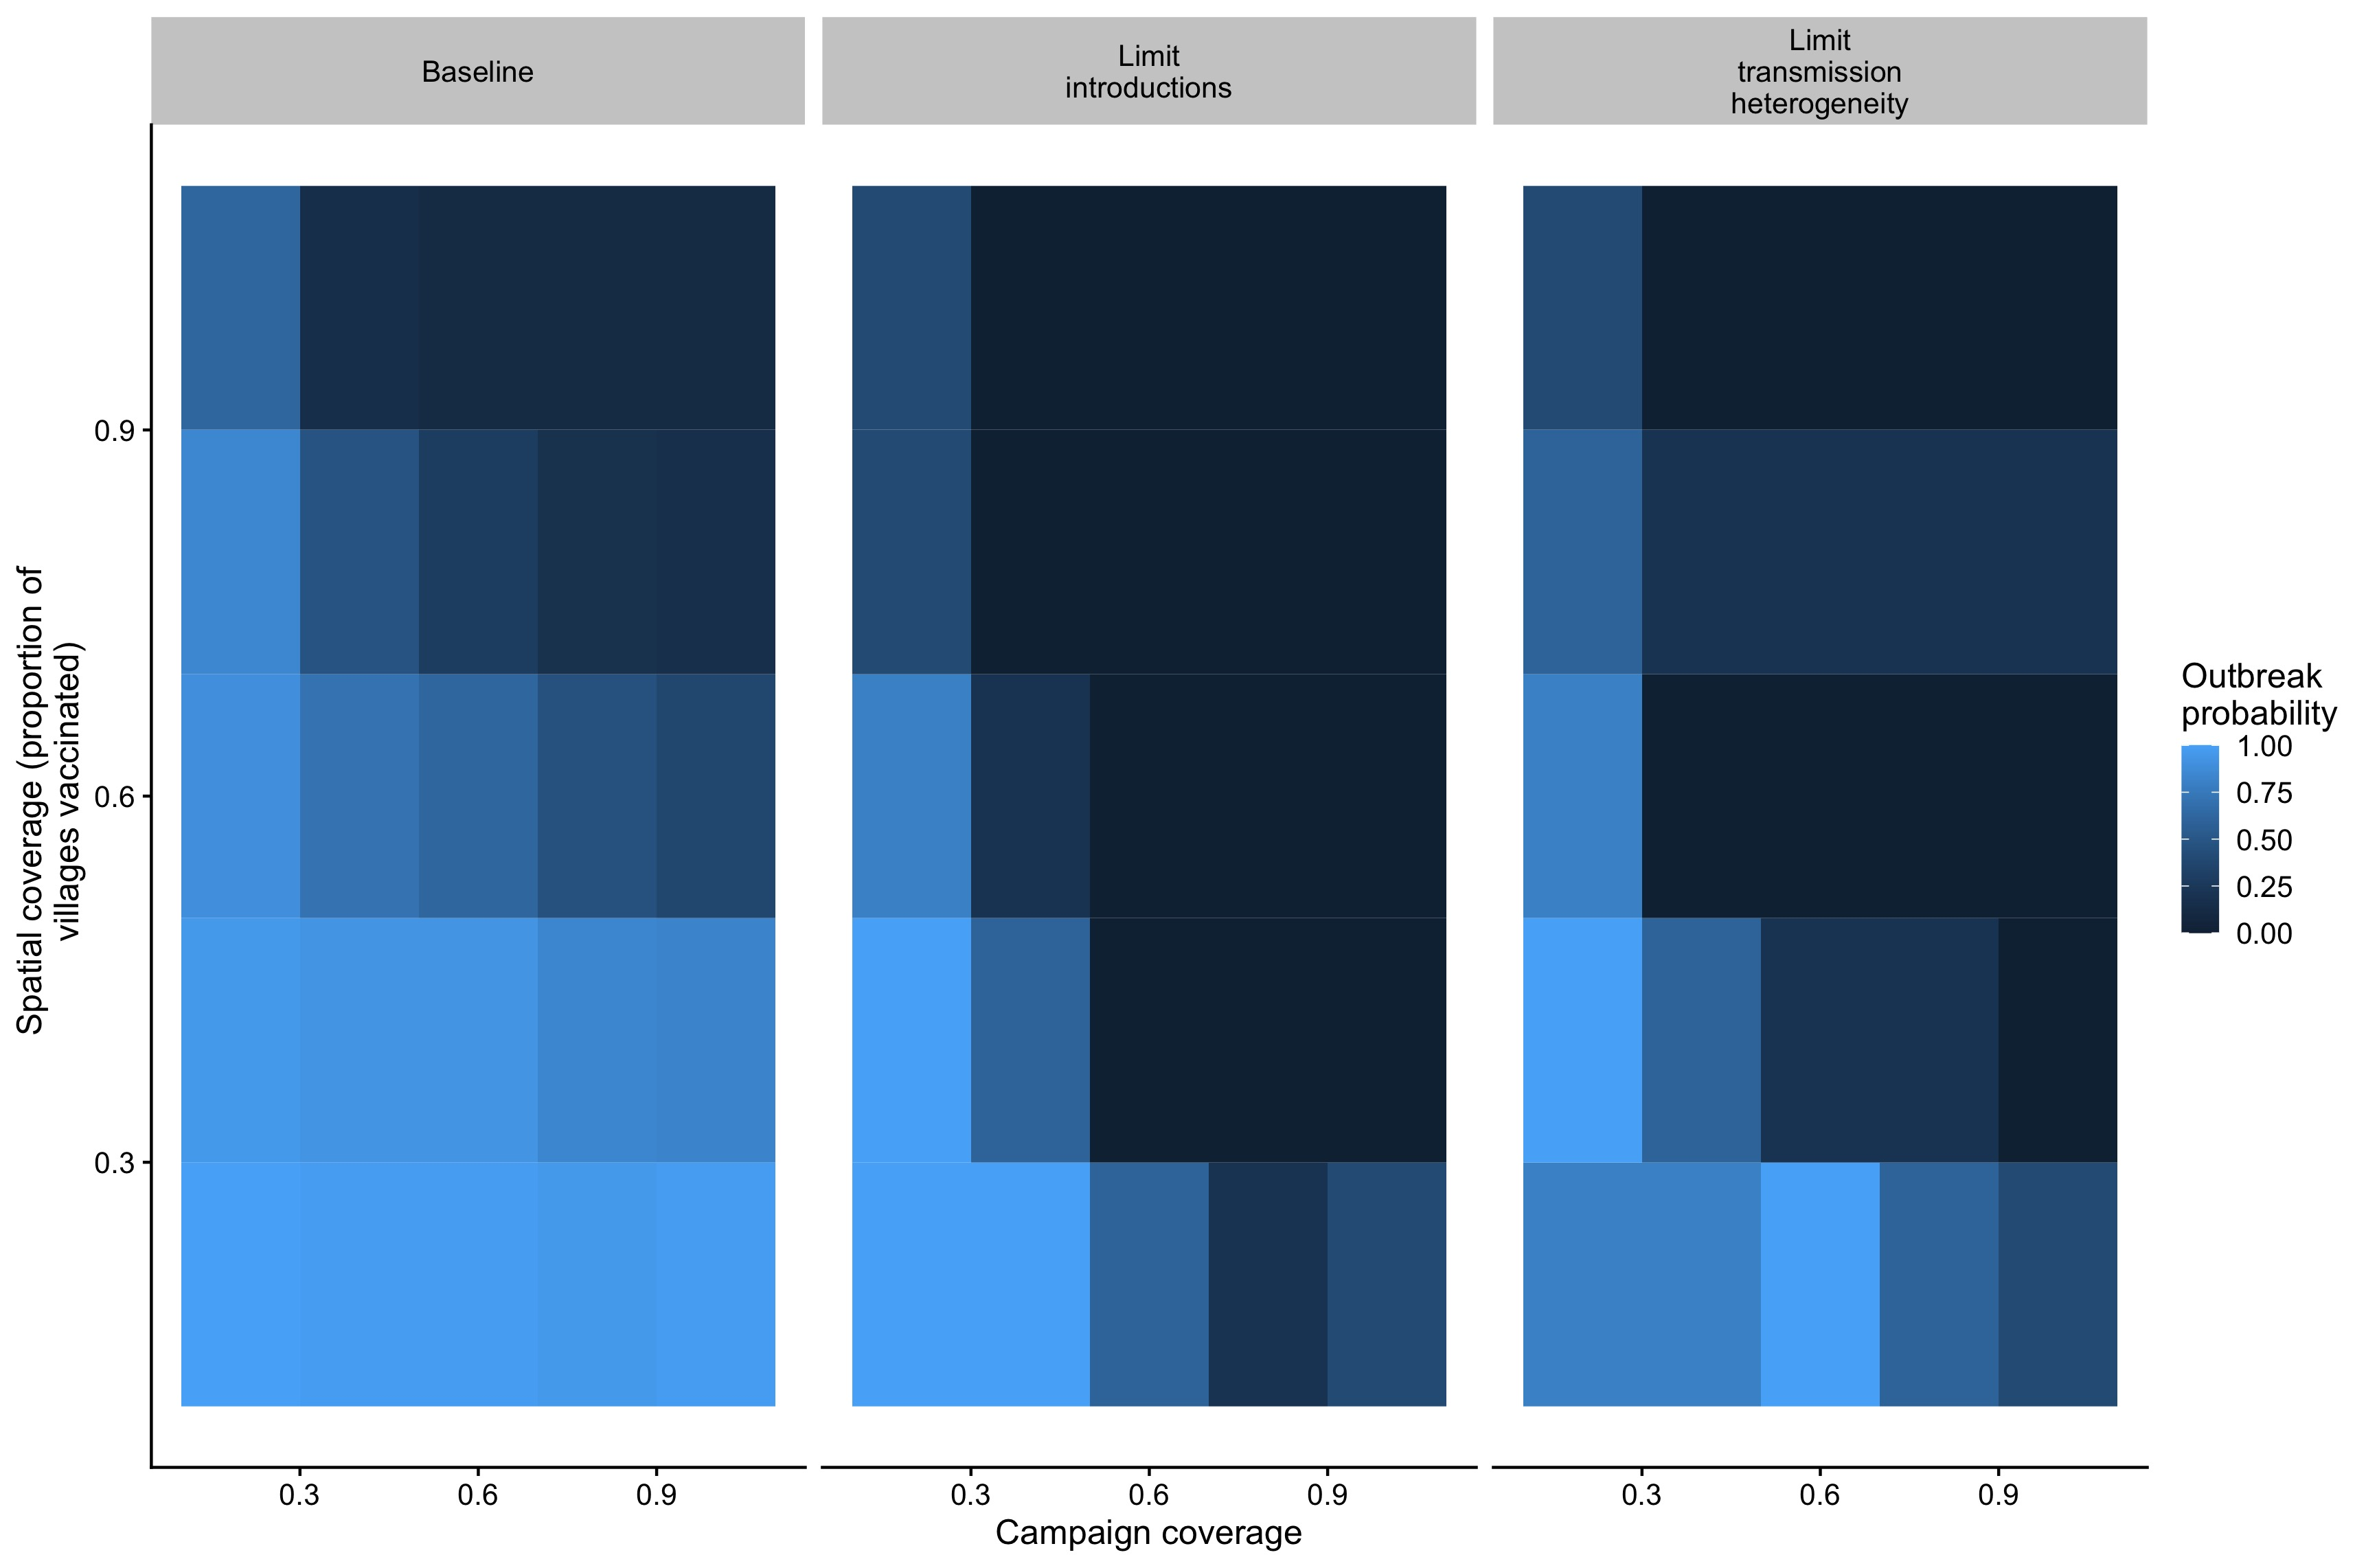
\includegraphics[width=0.9\linewidth]{/Users/mrajeev/Documents/Projects/dynamicSD/analysis/figs/mfig_int_comp} \caption[Outbreak probabilities across range of coverage and intervention scenarios.]{Outbreak probabilities (defined here as whether the number of consecutive weeks with cases above the 95th\% of the incursion rate exceeding 16 weeks) in relation to a range of campaign coverage and spatial coverage under the baseline scenario and with the additional limits on transmission heterogeneity and introductions.}\label{fig:mfig-int-comp}
\end{figure}



Two additional control strategies, one increasingly censoring transmission as coverage increases, approximating control strategies such as tracing and quarantine, and the second reducing the introduction rate as coverage is increased, approximating coordinated control efforts across larger geographic scales, also greatly improve control outcomes (Figs \ref{fig:sfig-incs-mets} and \ref{fig:sfig-sspread-mets}). In particular, reducing the introduction rate shifts both the spatial coverage and campaign coverage required to limit outbreaks (Fig \ref{fig:mfig-int-comp}).

\hypertarget{discussion-2}{%
\section{Discussion}\label{discussion-2}}

Overall, we find that accounting for both the spatial scale of vaccination and of mixing is critical to capturing the observed dynamics of canine rabies in the Serengeti District. Confirming previous work, we show that modeling transmission at the scale of dispersal (\textasciitilde{} 1km) is key to capturing stable endemic dynamics and also result in parameter estimates closest to empirical estimates from individual scale data. We also found that introductions of cases from outside the district are crucial to the maintenance of transmission. Importantly, spatial and spatiotemporal features of the data were key to differentiating between models and identifying parameter estimates, and the time series statistics of the data were generally the least predictive of model separation or parameter estimates. We find that high spatial coverage of vaccination campaigns is key to predicting control outcomes, even at a coarse administrative level. Here, we define \(R_{0}\) as the mean of the offspring distribution, but not as a critical threshold for persistence. Our results suggest that moving away from simplistic herd immunity thresholds to more nuanced targets, (i.e.~70\% of dogs in at least 70\% of villages), may better predict control outcomes. In addition, given the importance of transmission heterogeneity and introductions in transmission, control measures targeted at these key features, i.e.~coordinating control across larger geographic scales, could compound the dividends gained through vaccination alone.

We use a uniquely comprehensive data set in both temporal and spatial scope in our analysis. This data allow us to pin down key features and expectations of rabies transmission, and the vaccination and population data provide a lens into the underlying susceptible dynamics of the population. In addition, we have a strong empirical understanding of key epidemiological parameters governing rabies transmission (i.e.~incubation and infectious periods, dispersal kernels). Regardless of working with strong priors and in a narrow parameter space, certain parameters were still not identifiable, and no model was consistently able to predict the data observed. The dispersion parameter, or the heterogeneity in the transmission process was largely unidentifiable given our prior estimate, although it tended to be higher than estimates from empirical data, which could reflect issues of model misspecification, but could also result from biases in empirical data and direct estimates of this parameter \protect\hyperlink{ref-susswein2020}{{[}46{]}}.

Further refining summary statistics that draw the most information out of the available data may be a way forward to deal with these identifiability issues. However, given the stochastic nature of transmission dynamics, focusing on whether the observed data falls in the general trajectory space of the model may be the best we can do. The RF-ABC method is limited to estimation of independent parameter estimates, and we use a simple approach of filtering parameter sets where all weights are non-zero to approximate joint distributions. However, more work is needed to validate this approach, and other inference tools such as Sequential Monte Carlo methods could be used to estimate parameters jointly.

There are also uncertainties in the data that we did not account for. We use coarse demographic estimates at the village scale to simulate populations and do not account for immigration, emigration, or colonization of new patches. Our coverage estimates could be sensitive to these assumptions, although at the village scale, they generally track with estimates of vaccination coverage from post-vaccination surveys. In addition, we do not account for uncertainty in the case data in terms of timing and location of cases, and we use data on probable rather than laboratory confirmed rabies cases, although this approach has been shown to be highly specific in identifying genuine rabies cases \protect\hyperlink{ref-Hampson2009}{{[}33{]}}. We assume that case detection is high over this period, with approximately 85\% of cases detected each month. More work is needed to assess how sensitive our parameter estimates and model choice are to detection scenarios. Finally, our simulated control and vaccination scenarios are phenomenological and simplified approximations, rather than explicit representations of control programs.

Overall, we excluded many features of transmission included to explain dynamics in previous rabies modeling studies. We simulate secondary cases rather than biting rates and exposure probabilities \protect\hyperlink{ref-Mancyinprep}{{[}28{]}}, we do not account for human mediated dog movement within the district \protect\hyperlink{ref-ferguson2015}{{[}47{]}}, \protect\hyperlink{ref-townsend2013}{{[}48{]}}, we do not model the wildlife population \protect\hyperlink{ref-fitzpatrick2012}{{[}49{]}}, and finally we do not include reactive control to rabies outbreaks \protect\hyperlink{ref-ferguson2015}{{[}47{]}}, \protect\hyperlink{ref-townsend2013}{{[}48{]}}. However, many of these features are likely captured implicitly within this model. Human-mediated dog movements and wildlife cases may be captured in the introduction rate, and reactive control (that is human responses that are random rather than ones that scale with incidence) is likely captured in the dispersion parameter (i.e.~tying/killing/isolation of dogs resulting in failed transmission events). Here, we show that including these features explicitly may not be necessary when modeling transmission at the appropriate spatial scale and when incorporating key epidemiological features of the data such as transmission heterogeneity. Reactive control in particular, has often been used as a mechanism in previous models to generate realistic endemic dynamics and prevent host population declines, however there is little evidence that these measures scale temporally with incidence \protect\hyperlink{ref-Hampson2009}{{[}33{]}}. As the village level model did result in simulated trajectories matching our observed data, modeling dynamics at the scale of the control intervention may be sufficient to capture dynamics, and metapopulation models at the scale of control that approximate mixing could greatly reduce data barriers in implementing spatial models \protect\hyperlink{ref-pascual2011}{{[}50{]}}.

This work broadly confirms previous work on canine rabies transmission dynamics showing the importance of coverage heterogeneity in determining control outcomes and the spatial scale of mixing \protect\hyperlink{ref-Mancyinprep}{{[}28{]}}. Recent phylodynamic analyses of integrated sequence and epidemiological data have also highlighted the role of introductions from surrounding populations \protect\hyperlink{ref-zinsstag2017}{{[}51{]}}--\protect\hyperlink{ref-laager2019}{{[}53{]}}. These studies were largely at the scale of urban cities, and the authors argue that this indicates that rabies is not maintained within the population being studied. We find similar results in the Serengeti context, a less densely populated mosaic of agropastoralist communities. Together this work suggests that maintenance for canine rabies likely occurs across large spatial scales \protect\hyperlink{ref-hampson2007}{{[}54{]}}, and that low frequency events such as long-tailed disease induced dispersal or human mediated dog movement could facilitate this \protect\hyperlink{ref-talbi2010}{{[}24{]}}, \protect\hyperlink{ref-brunker2015}{{[}25{]}}. This has significant implications for control in that there are unlikely to be key sources or sink populations, or a critical community size for persistence \protect\hyperlink{ref-keeling1997}{{[}55{]}}. Rather, as phylogenetic analyses of cases from this district show, there are likely critical landscape structures over which rabies can persist \protect\hyperlink{ref-brunker2018}{{[}56{]}}.

Broadly, these results indicate the need to integrate key epidemiological features of transmission into dynamic models. We show that many aspects of transmission that have been included in previous models can be incorporated implicitly, and that modeling both the spatial scale of control and transmission is important for capturing observed dynamics under vaccination and stable endemic dynamics. Practically, developing spatial control targets may be a useful approach to improving the link between targets and outcomes and providing improved guidelines for vaccine implementation. However, more work should be done on how landscape and community structure impacts these outcomes. Moving forward, our work highlights the importance of confronting models with data and of incorporating key epidemiological features into models to generate realistic dynamics across the control timeline.

\hypertarget{references-4}{%
\section{References}\label{references-4}}

\setlength{\parskip}{1em}

\hypertarget{refs_main}{}
\begin{CSLReferences}{0}{0}
\leavevmode\hypertarget{ref-funk2020}{}%
\CSLLeftMargin{{[}1{]} }
\CSLRightInline{S. Funk and A. A. King, {``Choices and trade-offs in inference with infectious disease models,''} \emph{Epidemics}, vol. 30, p. 100383, Mar. 2020, doi: \href{https://doi.org/10.1016/j.epidem.2019.100383}{10.1016/j.epidem.2019.100383}.}

\leavevmode\hypertarget{ref-hampson2015}{}%
\CSLLeftMargin{{[}2{]} }
\CSLRightInline{K. Hampson \emph{et al.}, {``Estimating the global burden of endemic canine rabies.''} \emph{PLoS Neglected Tropical Diseases}, 2015.}

\leavevmode\hypertarget{ref-abela-ridder2016}{}%
\CSLLeftMargin{{[}3{]} }
\CSLRightInline{B. Abela-Ridder, L. Knopf, S. Martin, L. Taylor, G. Torres, and K. de Balogh, {``2016: The beginning of the end of rabies?''} \emph{The Lancet Global Health}, 2016.}

\leavevmode\hypertarget{ref-talbi2010}{}%
\CSLLeftMargin{{[}4{]} }
\CSLRightInline{C. Talbi \emph{et al.}, {``Phylodynamics and human-mediated dispersal of a zoonotic virus,''} \emph{PLoS Pathogens}, 2010.}

\leavevmode\hypertarget{ref-brunker2015}{}%
\CSLLeftMargin{{[}5{]} }
\CSLRightInline{K. Brunker \emph{et al.}, {``Elucidating the phylodynamics of endemic rabies virus in eastern africa using whole-genome sequencing.''} \emph{Virus Evolution}, 2015.}

\leavevmode\hypertarget{ref-rajeev2020modeling}{}%
\CSLLeftMargin{{[}6{]} }
\CSLRightInline{M. Rajeev, C. J. E. Metcalf, and K. Hampson, {``Modeling canine rabies virus transmission dynamics,''} in \emph{Rabies: 4th edition: Scientific basis of the disease and its management}, 2020.}

\leavevmode\hypertarget{ref-Mancyinprep}{}%
\CSLLeftMargin{{[}7{]} }
\CSLRightInline{Mancy Rebecca \emph{et al.}, {``Spatial scale of transmission explains how acute infections circulate at low prevalence.''}}

\leavevmode\hypertarget{ref-lankester2014}{}%
\CSLLeftMargin{{[}8{]} }
\CSLRightInline{F. Lankester, K. Hampson, T. Lembo, G. Palmer, L. Taylor, and S. Cleaveland, {``Implementing pasteur's vision for rabies elimination,''} \emph{Science}, 2014.}

\leavevmode\hypertarget{ref-scott2017}{}%
\CSLLeftMargin{{[}9{]} }
\CSLRightInline{T. P. Scott, A. Coetzer, A. S. Fahrion, and L. H. Nel, {``Addressing the disconnect between the estimated, reported, and true rabies data: The development of a regional african rabies bulletin,''} \emph{Frontiers in veterinary science}, 2017.}

\leavevmode\hypertarget{ref-townsend2013a}{}%
\CSLLeftMargin{{[}10{]} }
\CSLRightInline{S. E. Townsend \emph{et al.}, {``Surveillance guidelines for disease elimination: A case study of canine rabies,''} \emph{Comparative Immunology, Microbiology and Infectious Diseases}, vol. 36, no. 3, pp. 249--261, May 2013, doi: \href{https://doi.org/10.1016/j.cimid.2012.10.008}{10.1016/j.cimid.2012.10.008}.}

\leavevmode\hypertarget{ref-hazelbag2020}{}%
\CSLLeftMargin{{[}11{]} }
\CSLRightInline{C. M. Hazelbag, J. Dushoff, E. M. Dominic, Z. E. Mthombothi, and W. Delva, {``Calibration of individual-based models to epidemiological data: A systematic review,''} \emph{PLOS Computational Biology}, vol. 16, no. 5, p. e1007893, May 2020, doi: \href{https://doi.org/10.1371/journal.pcbi.1007893}{10.1371/journal.pcbi.1007893}.}

\leavevmode\hypertarget{ref-Hampson2009}{}%
\CSLLeftMargin{{[}12{]} }
\CSLRightInline{K. Hampson \emph{et al.}, {``Transmission Dynamics and Prospects for the Elimination of Canine Rabies,''} \emph{PLoS Biology}, vol. 7, no. 3, p. e1000053, Mar. 2009, doi: \href{https://doi.org/10.1371/journal.pbio.1000053}{10.1371/journal.pbio.1000053}.}

\leavevmode\hypertarget{ref-czupryna2016}{}%
\CSLLeftMargin{{[}13{]} }
\CSLRightInline{A. M. Czupryna \emph{et al.}, {``Ecology and demography of free-roaming domestic dogs in rural villages near serengeti national park in tanzania,''} \emph{PLoS ONE}, 2016.}

\leavevmode\hypertarget{ref-pudlo2015}{}%
\CSLLeftMargin{{[}14{]} }
\CSLRightInline{P. Pudlo, J.-M. Marin, A. Estoup, J.-M. Cornuet, M. Gautier, and C. P. Robert, {``Reliable ABC model choice via random forests,''} \emph{Bioinformatics}, vol. 32, no. 6, pp. 859--866, Nov. 2015, doi: \href{https://doi.org/10.1093/bioinformatics/btv684}{10.1093/bioinformatics/btv684}.}

\leavevmode\hypertarget{ref-raynal2018}{}%
\CSLLeftMargin{{[}15{]} }
\CSLRightInline{L. Raynal, J.-M. Marin, P. Pudlo, M. Ribatet, C. P. Robert, and A. Estoup, {``ABC random forests for Bayesian parameter inference,''} \emph{Bioinformatics}, vol. 35, no. 10, pp. 1720--1728, Oct. 2018, doi: \href{https://doi.org/10.1093/bioinformatics/bty867}{10.1093/bioinformatics/bty867}.}

\leavevmode\hypertarget{ref-jordan2019}{}%
\CSLLeftMargin{{[}16{]} }
\CSLRightInline{A. Jordan, F. Krüger, and S. Lerch, {``Evaluating Probabilistic Forecasts with scoringRules,''} \emph{Journal of Statistical Software}, vol. 90, no. 12, 2019, doi: \href{https://doi.org/10.18637/jss.v090.i12}{10.18637/jss.v090.i12}.}

\leavevmode\hypertarget{ref-juul2020}{}%
\CSLLeftMargin{{[}17{]} }
\CSLRightInline{J. L. Juul, K. Græsbøll, L. E. Christiansen, and S. Lehmann, {``Fixed-time descriptive statistics underestimate extremes of epidemic curve ensembles,''} \emph{Nature Physics}, vol. 17, no. 1, pp. 5--8, Dec. 2020, doi: \href{https://doi.org/10.1038/s41567-020-01121-y}{10.1038/s41567-020-01121-y}.}

\leavevmode\hypertarget{ref-Kain2020}{}%
\CSLLeftMargin{{[}18{]} }
\CSLRightInline{M. P. Kain, M. L. Childs, A. D. Becker, and E. A. Mordecai, {``Chopping the tail: How preventing superspreading can help to maintain COVID-19 control.''} Jul. 03, 2020, doi: \href{https://doi.org/10.1101/2020.06.30.20143115}{10.1101/2020.06.30.20143115}.}

\leavevmode\hypertarget{ref-R-program}{}%
\CSLLeftMargin{{[}19{]} }
\CSLRightInline{R Core Team, \emph{R: A language and environment for statistical computing}. Vienna, Austria: R Foundation for Statistical Computing, 2020.}

\leavevmode\hypertarget{ref-R-sf}{}%
\CSLLeftMargin{{[}20{]} }
\CSLRightInline{E. Pebesma, \emph{Sf: Simple features for r}. 2021.}

\leavevmode\hypertarget{ref-R-data.table}{}%
\CSLLeftMargin{{[}21{]} }
\CSLRightInline{M. Dowle and A. Srinivasan, \emph{Data.table: Extension of `data.frame`}. 2020.}

\leavevmode\hypertarget{ref-R-ranger}{}%
\CSLLeftMargin{{[}22{]} }
\CSLRightInline{M. N. Wright, S. Wager, and P. Probst, \emph{Ranger: A fast implementation of random forests}. 2020.}

\leavevmode\hypertarget{ref-R-raster}{}%
\CSLLeftMargin{{[}23{]} }
\CSLRightInline{R. J. Hijmans, \emph{Raster: Geographic data analysis and modeling}. 2020.}

\leavevmode\hypertarget{ref-R-foreach}{}%
\CSLLeftMargin{{[}24{]} }
\CSLRightInline{Revolution Analytics and S. Weston, \emph{Foreach: Provides foreach looping construct}.}

\leavevmode\hypertarget{ref-susswein2020}{}%
\CSLLeftMargin{{[}25{]} }
\CSLRightInline{Z. Susswein and S. Bansal, {``Characterizing superspreading of SARS-CoV-2 : From mechanism to measurement.''} Dec. 11, 2020, doi: \href{https://doi.org/10.1101/2020.12.08.20246082}{10.1101/2020.12.08.20246082}.}

\leavevmode\hypertarget{ref-ferguson2015}{}%
\CSLLeftMargin{{[}26{]} }
\CSLRightInline{E. A. Ferguson \emph{et al.}, {``Heterogeneity in the spread and control of infectious disease: Consequences for the elimination of canine rabies,''} \emph{Nature Publishing Group}, 2015.}

\leavevmode\hypertarget{ref-townsend2013}{}%
\CSLLeftMargin{{[}27{]} }
\CSLRightInline{S. E. Townsend \emph{et al.}, {``Designing programs for eliminating canine rabies from islands: Bali, indonesia as a case study.''} \emph{PLoS Neglected Tropical Diseases}, 2013.}

\leavevmode\hypertarget{ref-fitzpatrick2012}{}%
\CSLLeftMargin{{[}28{]} }
\CSLRightInline{M. C. Fitzpatrick, K. Hampson, S. Cleaveland, L. A. Meyers, J. P. Townsend, and A. P. Galvani, {``Potential for rabies control through dog vaccination in wildlife-abundant communities of tanzania,''} \emph{PLoS Neglected Tropical Diseases}, 2012.}

\leavevmode\hypertarget{ref-pascual2011}{}%
\CSLLeftMargin{{[}29{]} }
\CSLRightInline{M. Pascual, M. Roy, and K. Laneri, {``Simple models for complex systems: Exploiting the relationship between local and global densities,''} \emph{Theoretical Ecology}, 2011.}

\leavevmode\hypertarget{ref-zinsstag2017}{}%
\CSLLeftMargin{{[}30{]} }
\CSLRightInline{J. Zinsstag \emph{et al.}, {``Vaccination of dogs in an african city interrupts rabies transmission and reduces human exposure.''} \emph{Science translational medicine}, 2017.}

\leavevmode\hypertarget{ref-bourhy2016}{}%
\CSLLeftMargin{{[}31{]} }
\CSLRightInline{H. Bourhy \emph{et al.}, {``Revealing the micro-scale signature of endemic zoonotic disease transmission in an african urban setting,''} \emph{PLoS Pathogens}, 2016.}

\leavevmode\hypertarget{ref-laager2019}{}%
\CSLLeftMargin{{[}32{]} }
\CSLRightInline{M. Laager \emph{et al.}, {``A metapopulation model of dog rabies transmission in n'djamena, chad,''} \emph{Journal of Theoretical Biology}, 2019.}

\leavevmode\hypertarget{ref-hampson2007}{}%
\CSLLeftMargin{{[}33{]} }
\CSLRightInline{K. Hampson, J. Dushoff, J. Bingham, G. Brückner, Y. H. Ali, and A. Dobson, {``Synchronous cycles of domestic dog rabies in sub-saharan africa and the impact of control efforts.''} \emph{Proceedings of the National Academy of Sciences}, 2007.}

\leavevmode\hypertarget{ref-keeling1997}{}%
\CSLLeftMargin{{[}34{]} }
\CSLRightInline{M. J. Keeling, {``Disease extinction and community size: Modeling the persistence of measles,''} \emph{Science}, vol. 275, no. 5296, pp. 65--67, Jan. 1997, doi: \href{https://doi.org/10.1126/science.275.5296.65}{10.1126/science.275.5296.65}.}

\leavevmode\hypertarget{ref-brunker2018}{}%
\CSLLeftMargin{{[}35{]} }
\CSLRightInline{K. Brunker \emph{et al.}, {``Landscape attributes governing local transmission of an endemic zoonosis: Rabies virus in domestic dogs,''} \emph{Molecular Ecology}, 2018.}

\leavevmode\hypertarget{ref-ranger2017}{}%
\CSLLeftMargin{{[}36{]} }
\CSLRightInline{M. N. Wright and A. Ziegler, {``{ranger}: A fast implementation of random forests for high dimensional data in {C++} and {R},''} \emph{Journal of Statistical Software}, vol. 77, no. 1, pp. 1--17, 2017, doi: \href{https://doi.org/10.18637/jss.v077.i01}{10.18637/jss.v077.i01}.}

\leavevmode\hypertarget{ref-sf2018}{}%
\CSLLeftMargin{{[}37{]} }
\CSLRightInline{E. Pebesma, {``{Simple Features for R: Standardized Support for Spatial Vector Data},''} \emph{{The R Journal}}, vol. 10, no. 1, pp. 439--446, 2018, doi: \href{https://doi.org/10.32614/RJ-2018-009}{10.32614/RJ-2018-009}.}

\end{CSLReferences}

\newpage

\hypertarget{supplementary-figures-1}{%
\section{Supplementary Figures}\label{supplementary-figures-1}}

\beginsupplement

\setlength{\parskip}{2em}

\begin{figure}
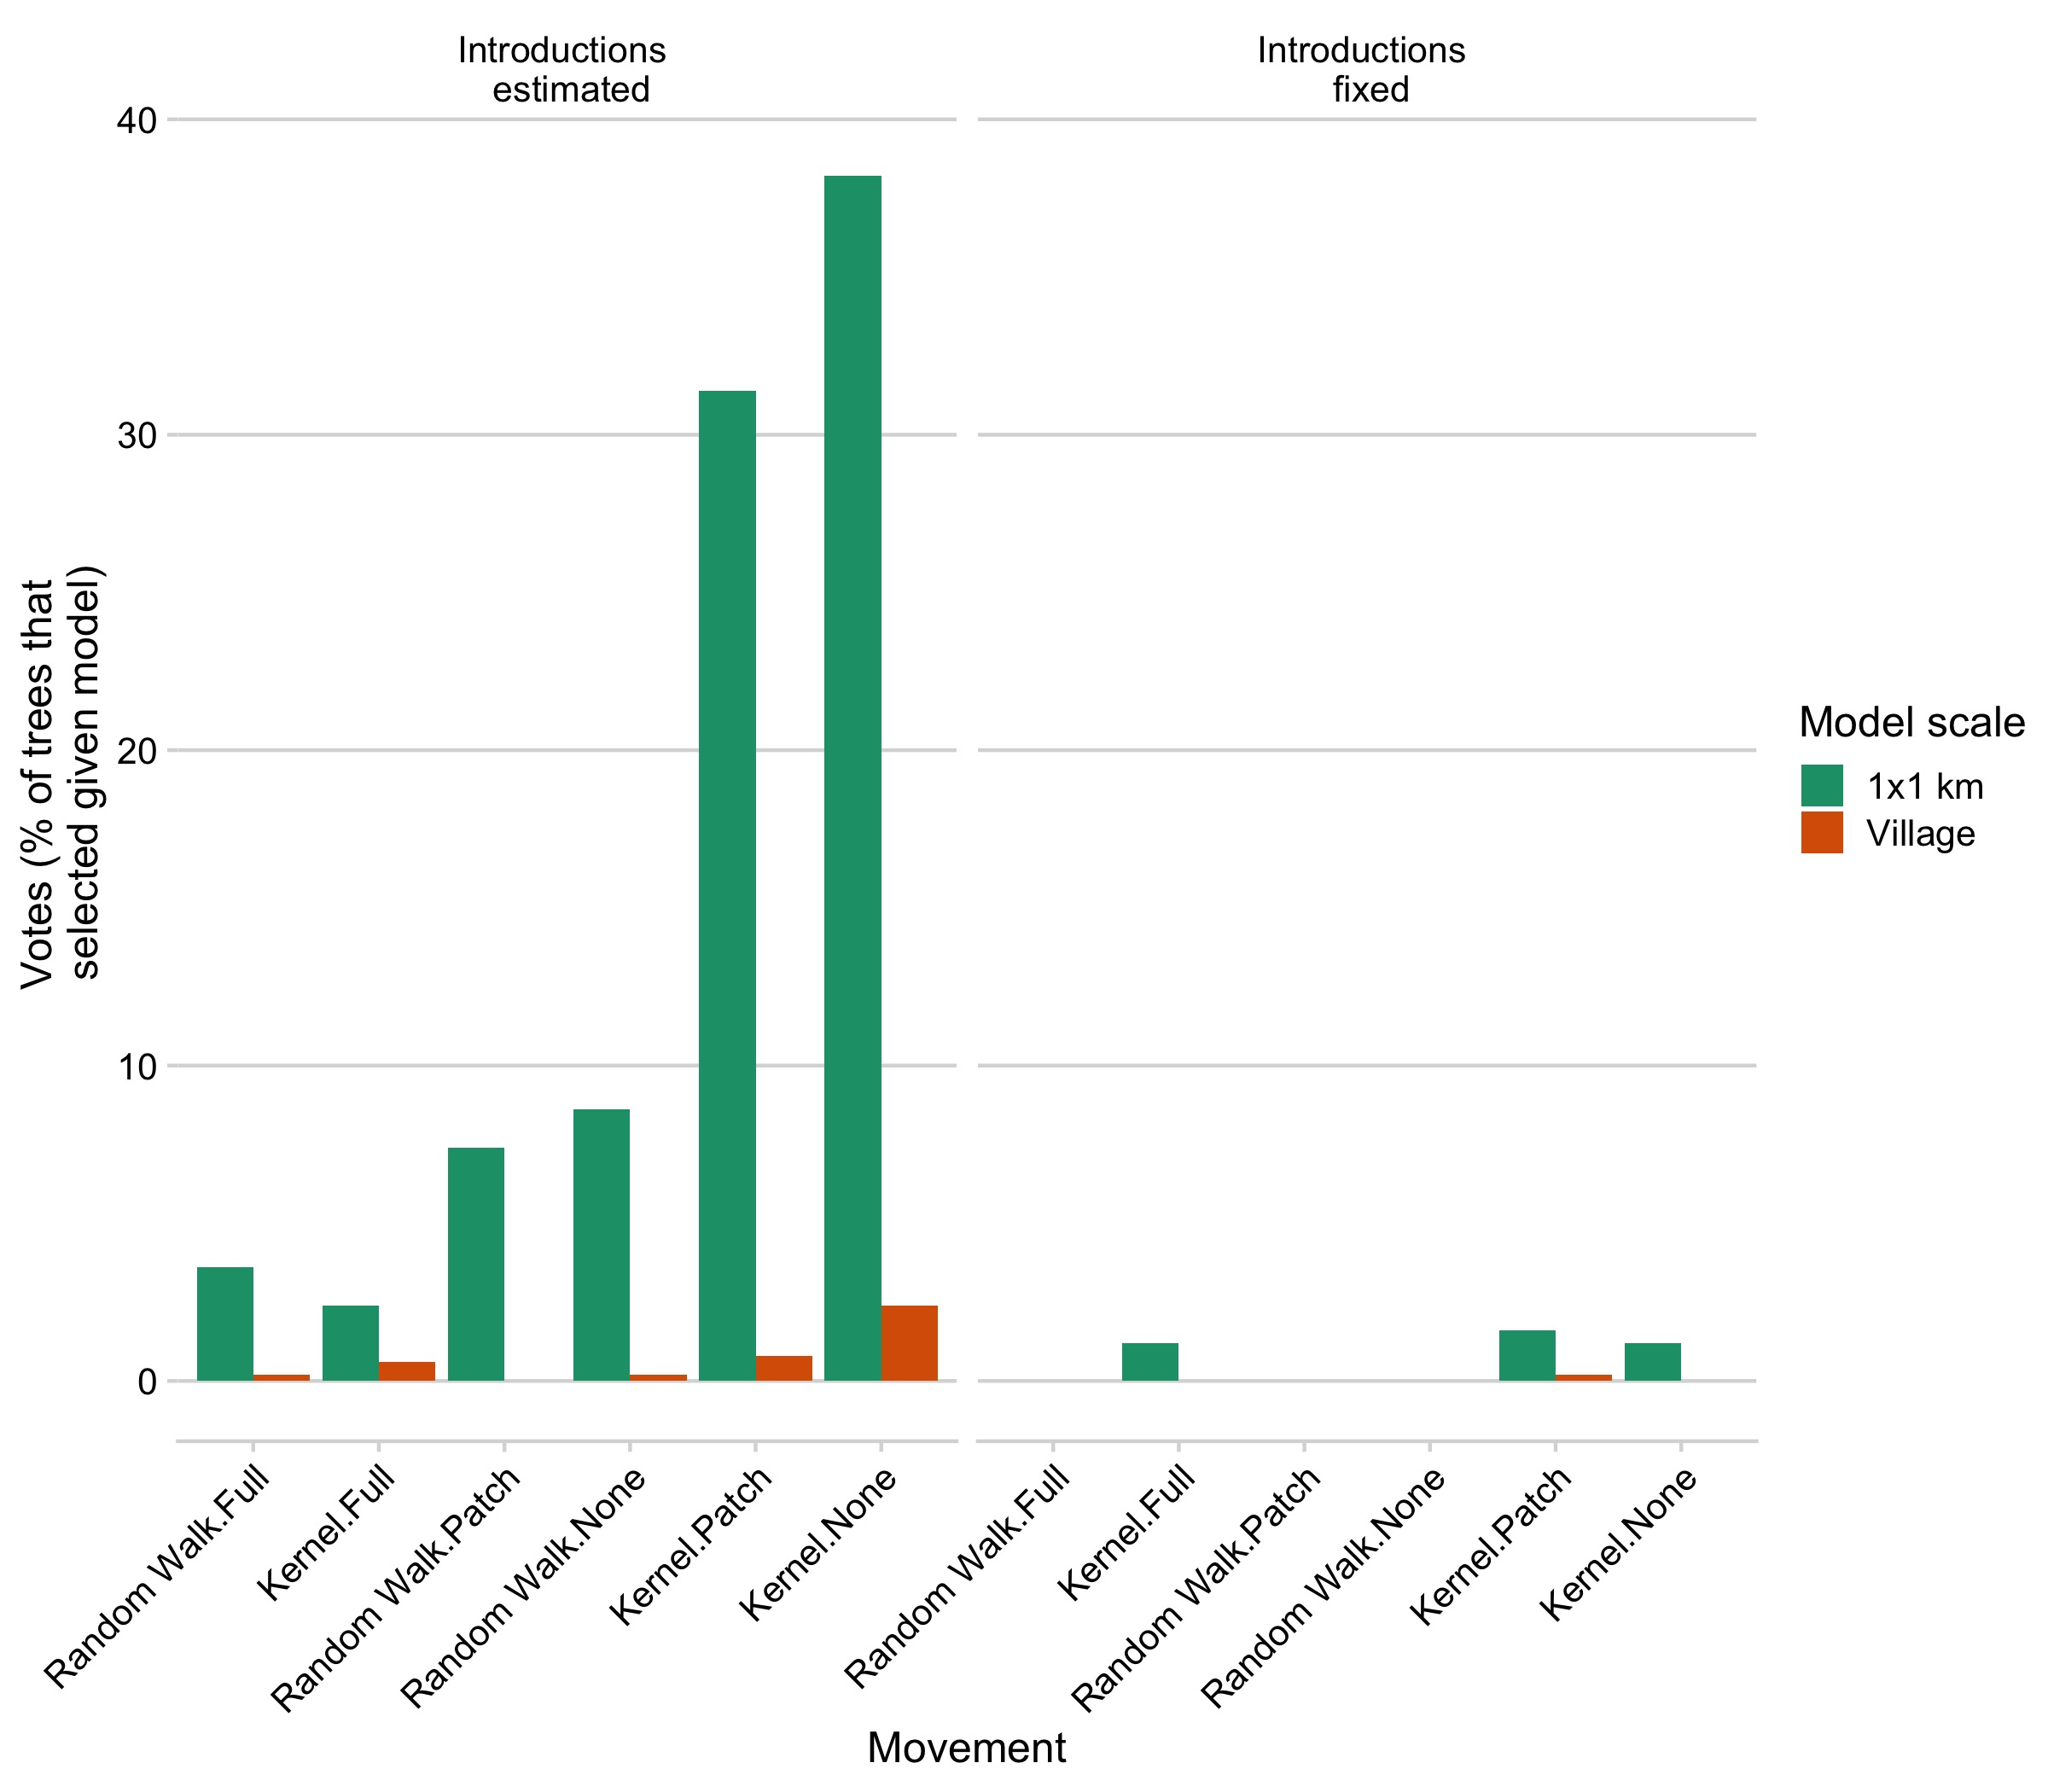
\includegraphics[width=0.9\linewidth]{/Users/mrajeev/Documents/Projects/dynamicSD/analysis/figs/sfig_mod_ranks} \caption[Posterior probability of models given observed data.]{Posterior probability of each model given our observed data, with the panels comparing models with fixed vs.~estimated introductions, the colors showing the model scale, and the x-axis how movement was specified (see Methods).}\label{fig:sfig-mod-ranks}
\end{figure}



\begin{figure}
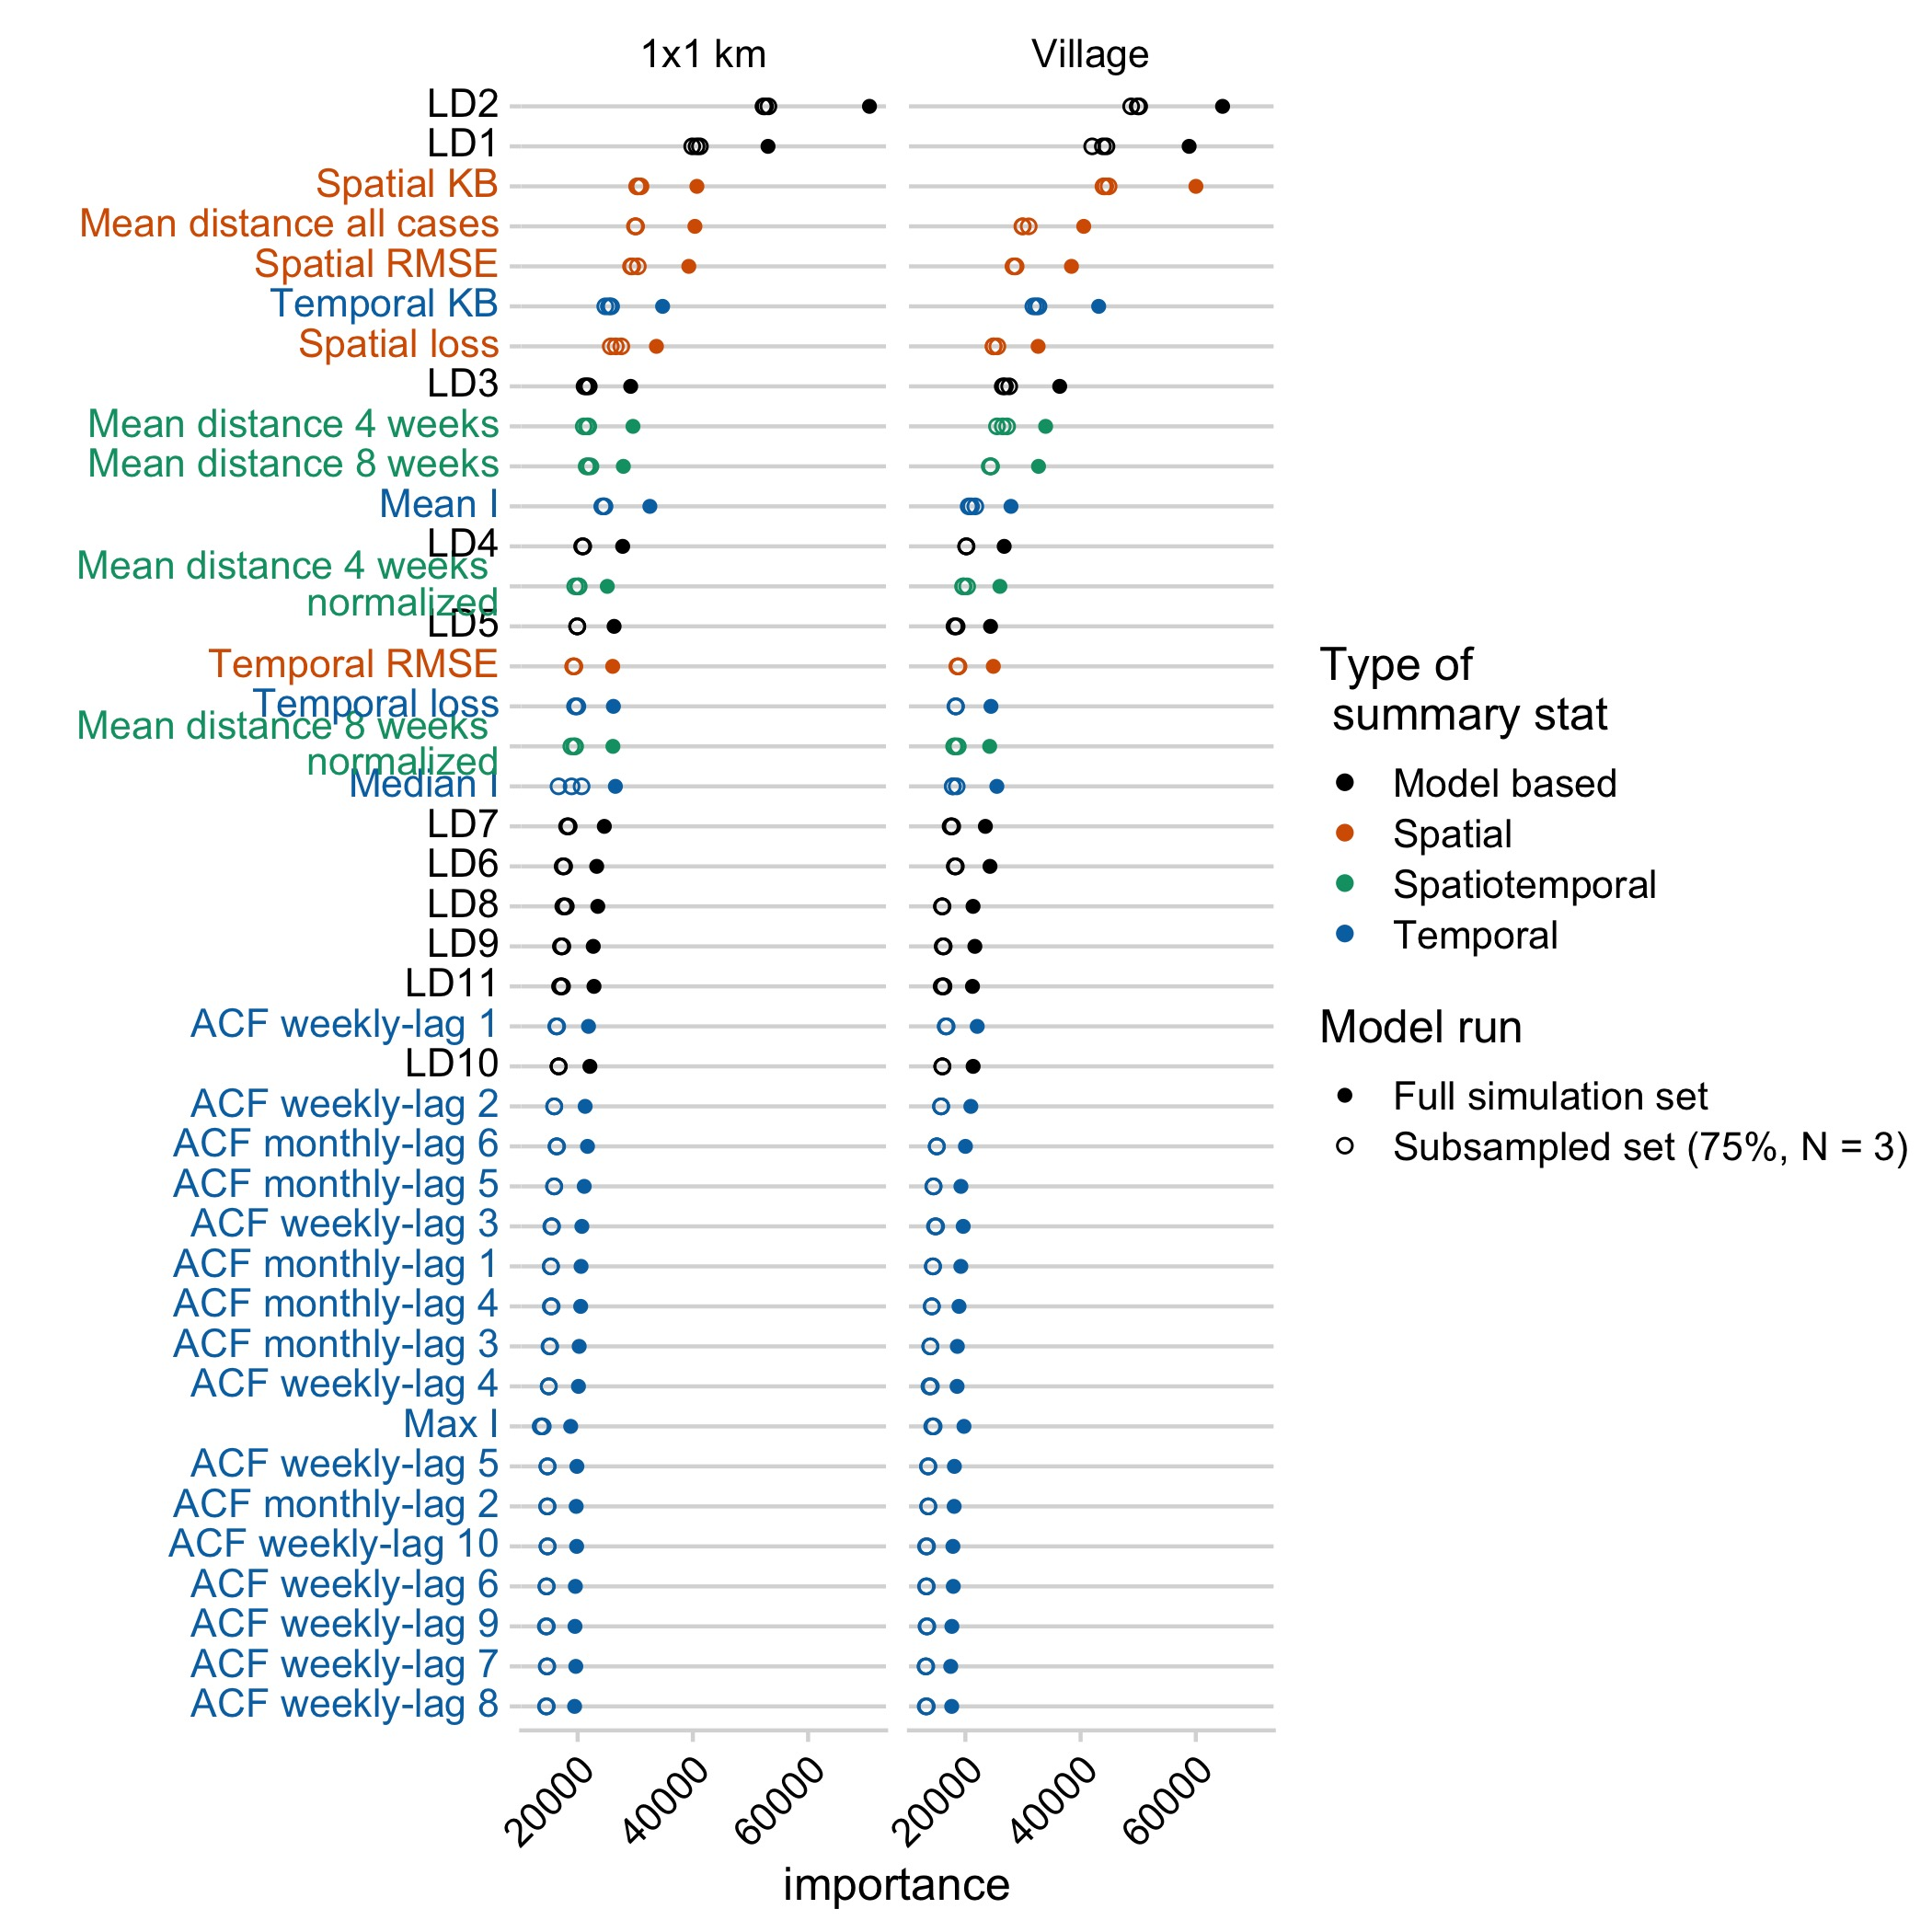
\includegraphics[width=0.9\linewidth]{/Users/mrajeev/Documents/Projects/dynamicSD/analysis/figs/sfig_mod_vimp} \caption[Variable importance plots for parameters with full or subsampled simulations.]{Variable importance plots for models run with the full simulation data set (N = 1e5 simulations per model), or subsampled datasets (approx. 75\% of the full simulation data set).}\label{fig:sfig-mod-vimp}
\end{figure}



\begin{figure}
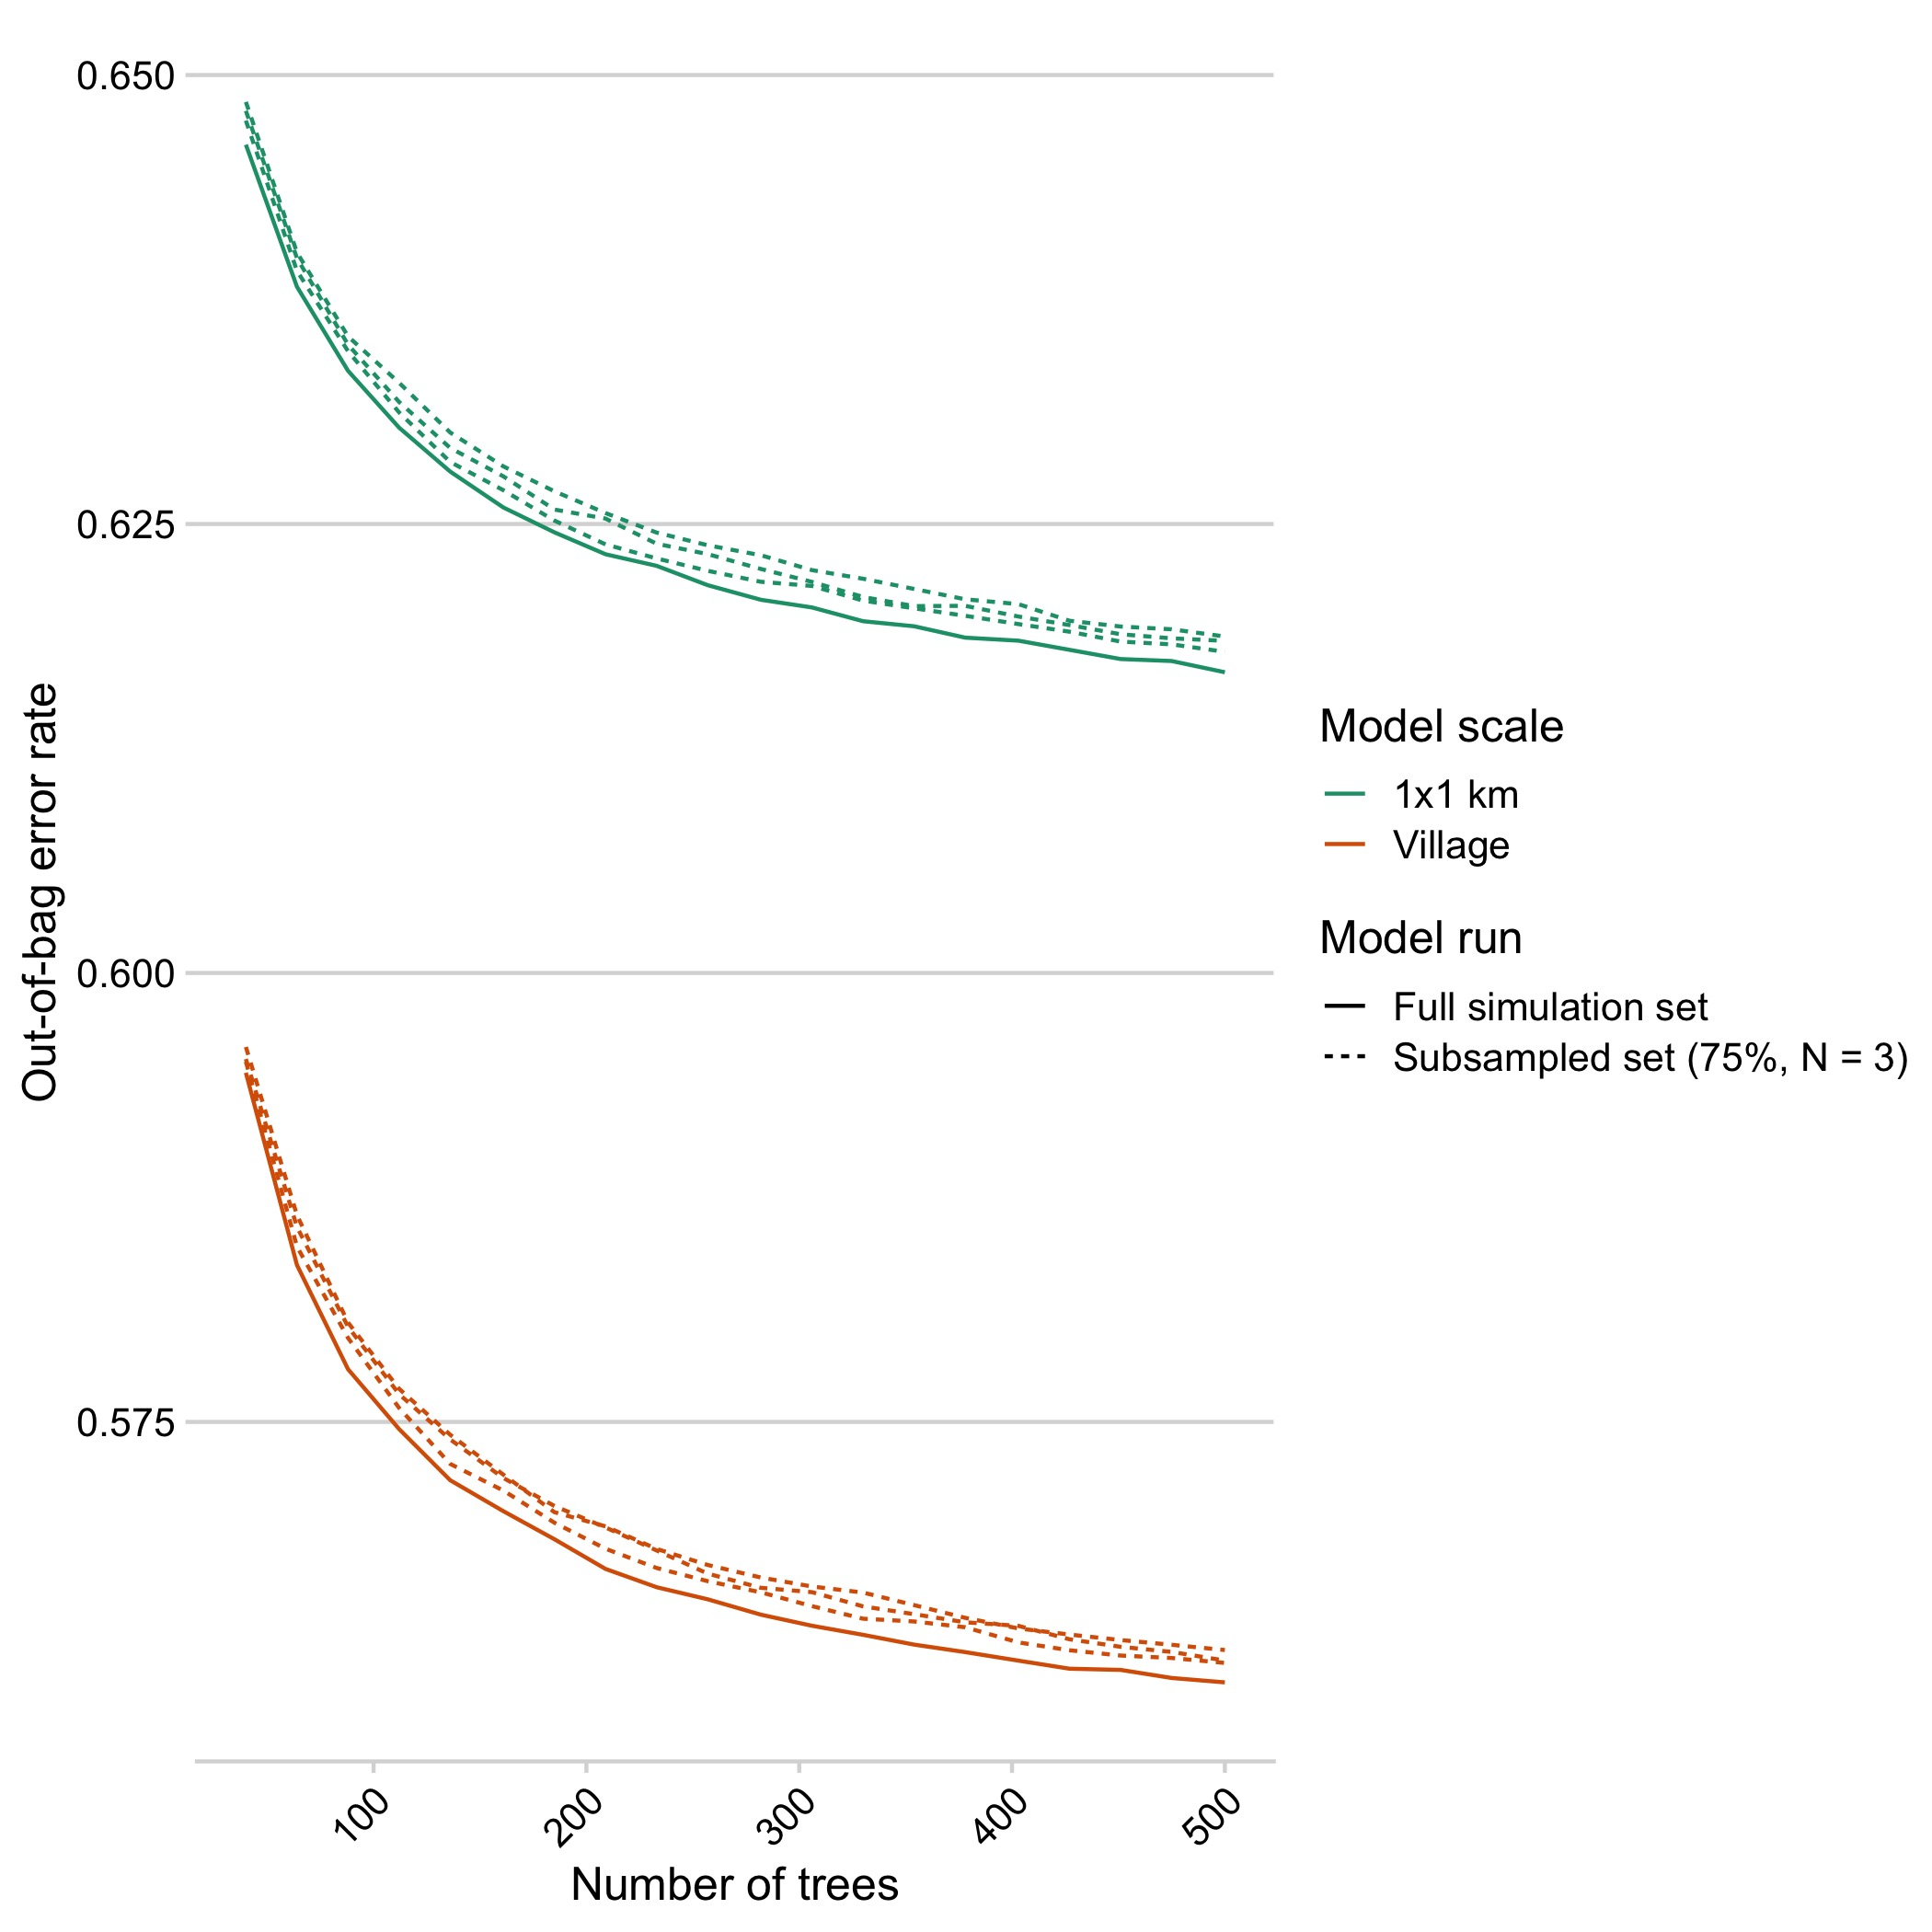
\includegraphics[width=0.9\linewidth]{/Users/mrajeev/Documents/Projects/dynamicSD/analysis/figs/sfig_mod_err} \caption{Out-of-bag predictions of the out-of-bag error rate as trees are added separated by the scale of the model comparison.}\label{fig:sfig-mod-err}
\end{figure}



\begin{figure}
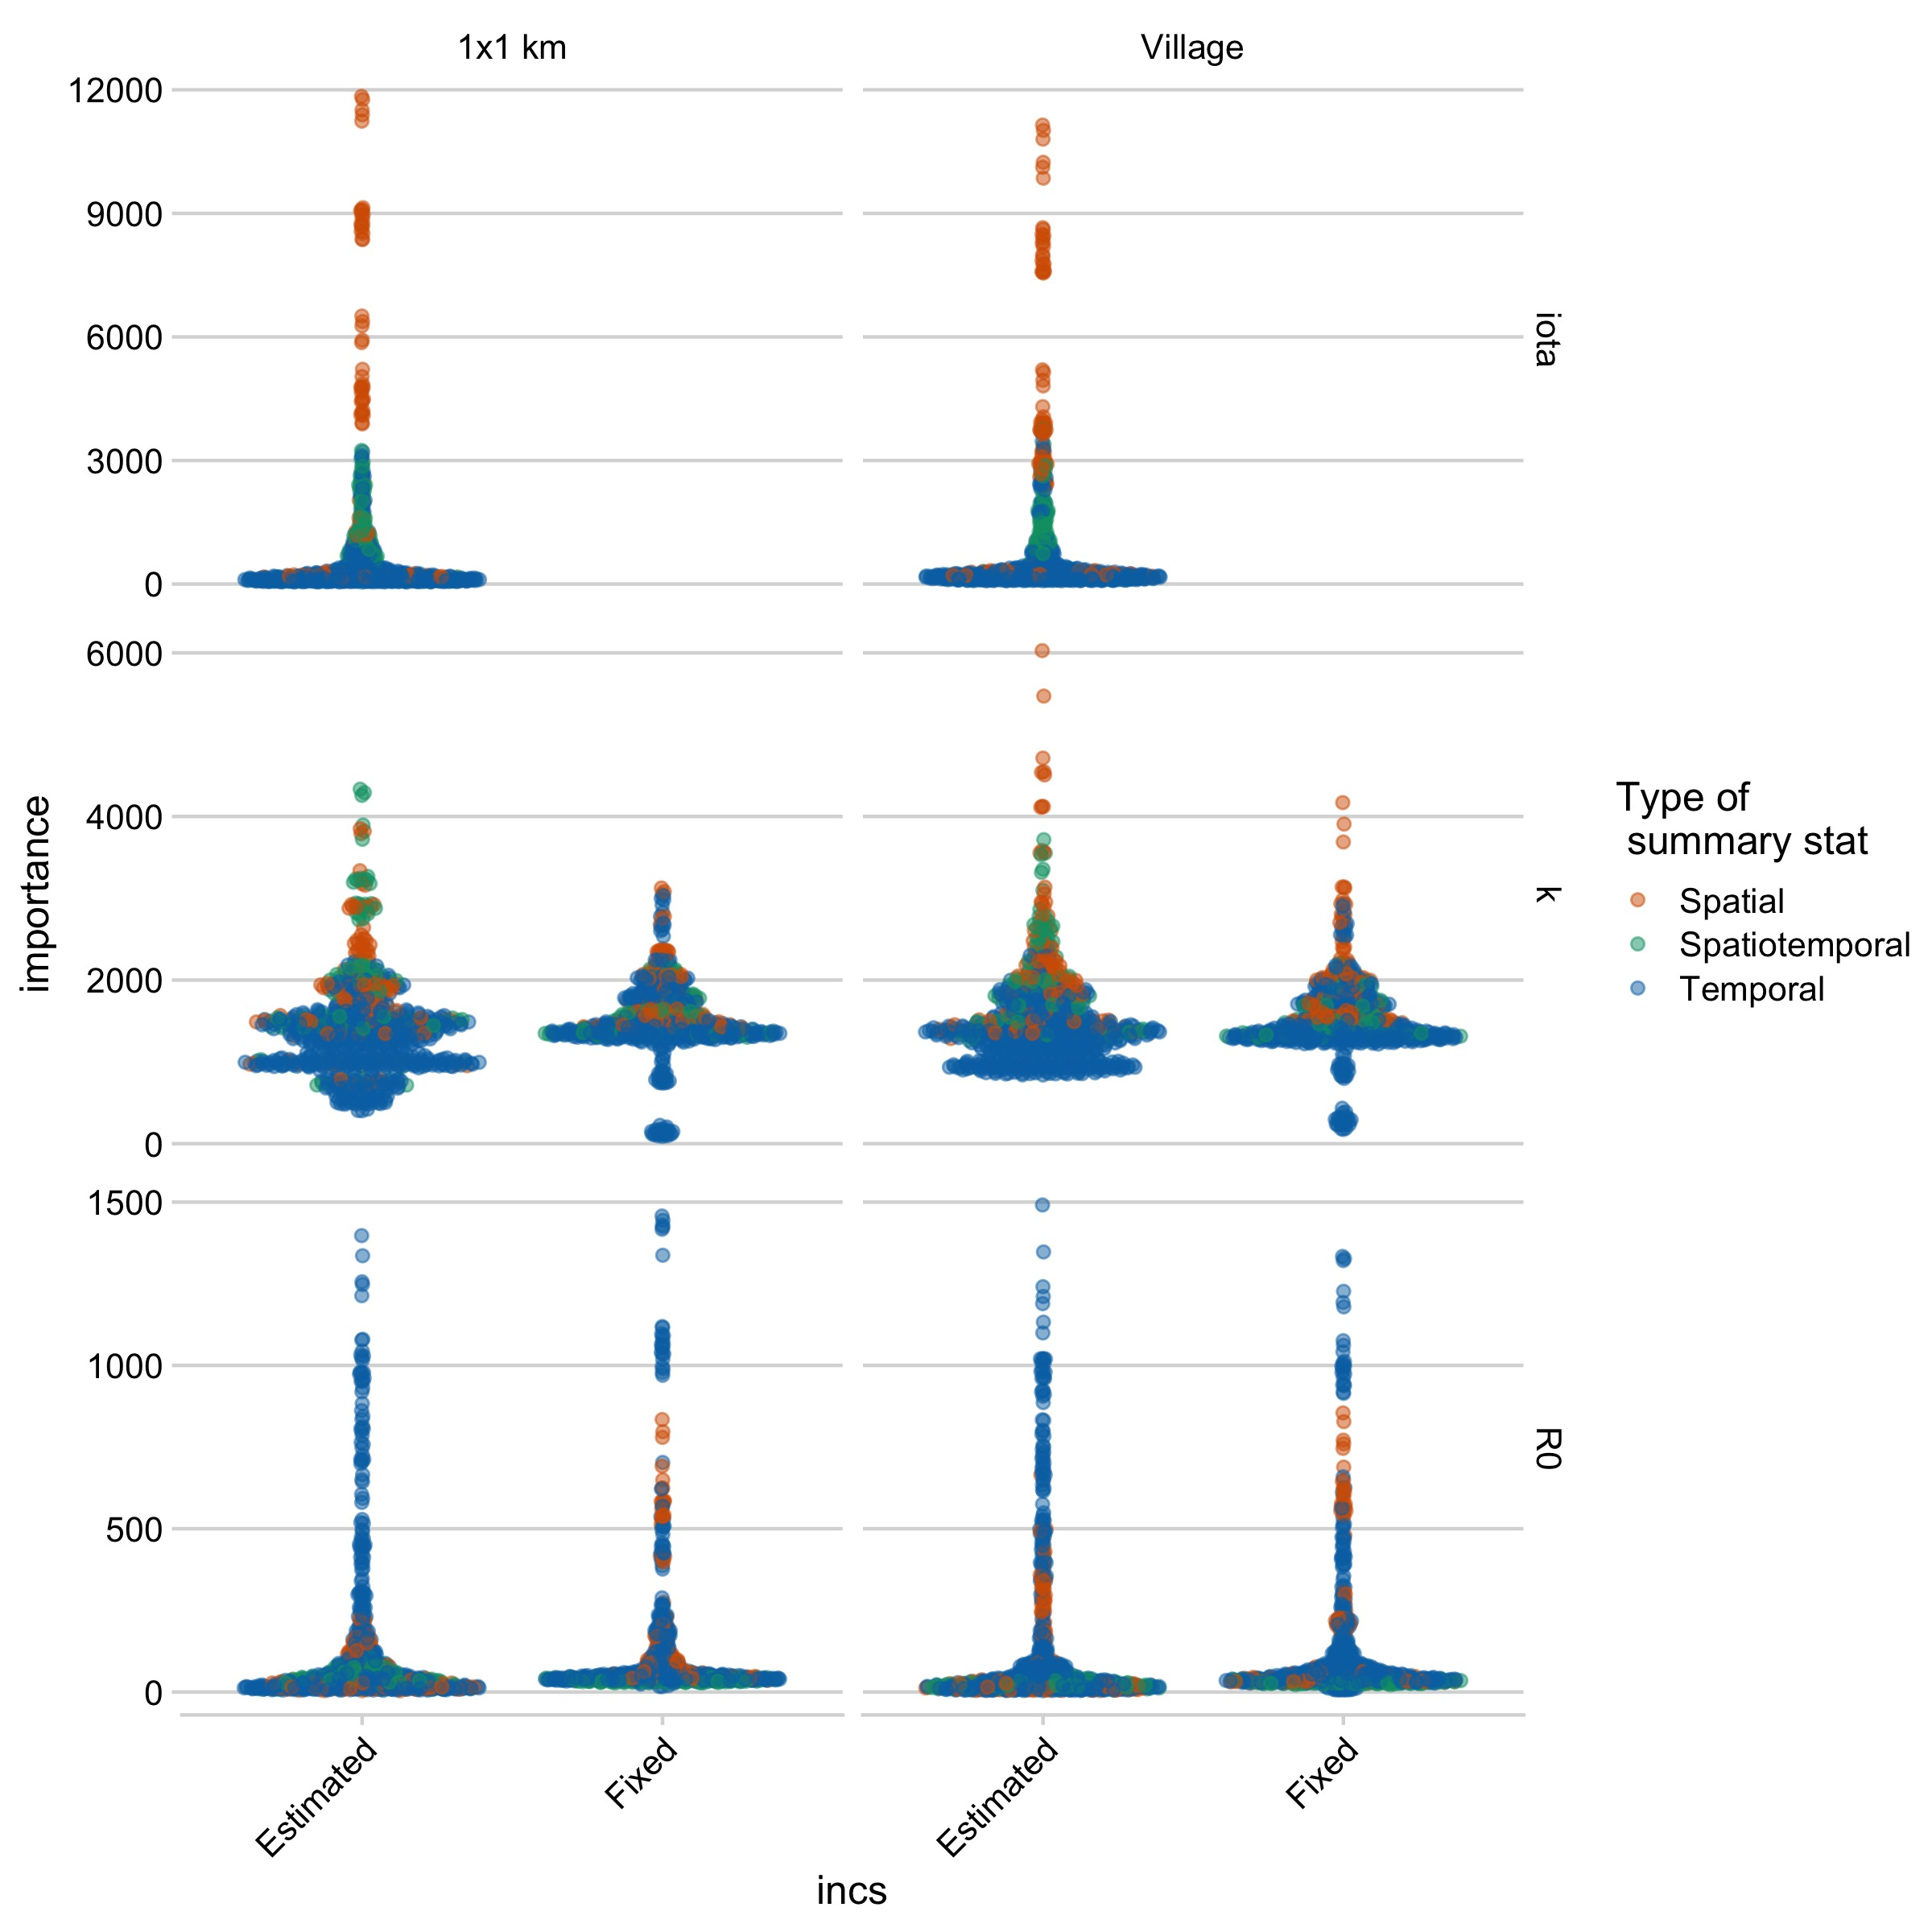
\includegraphics[width=0.9\linewidth]{/Users/mrajeev/Documents/Projects/dynamicSD/analysis/figs/sfig_posts_vimpgr} \caption[Variable importance plots for parameters with full or subsampled simulations.]{Variable importance plots for models run with the full simulation data set (N = 1e5 simulations per model), or subsampled datasets (approx. 75\% of the full simulation data set) for each parameter and model.}\label{fig:sfig-posts-vimp}
\end{figure}



\begin{figure}
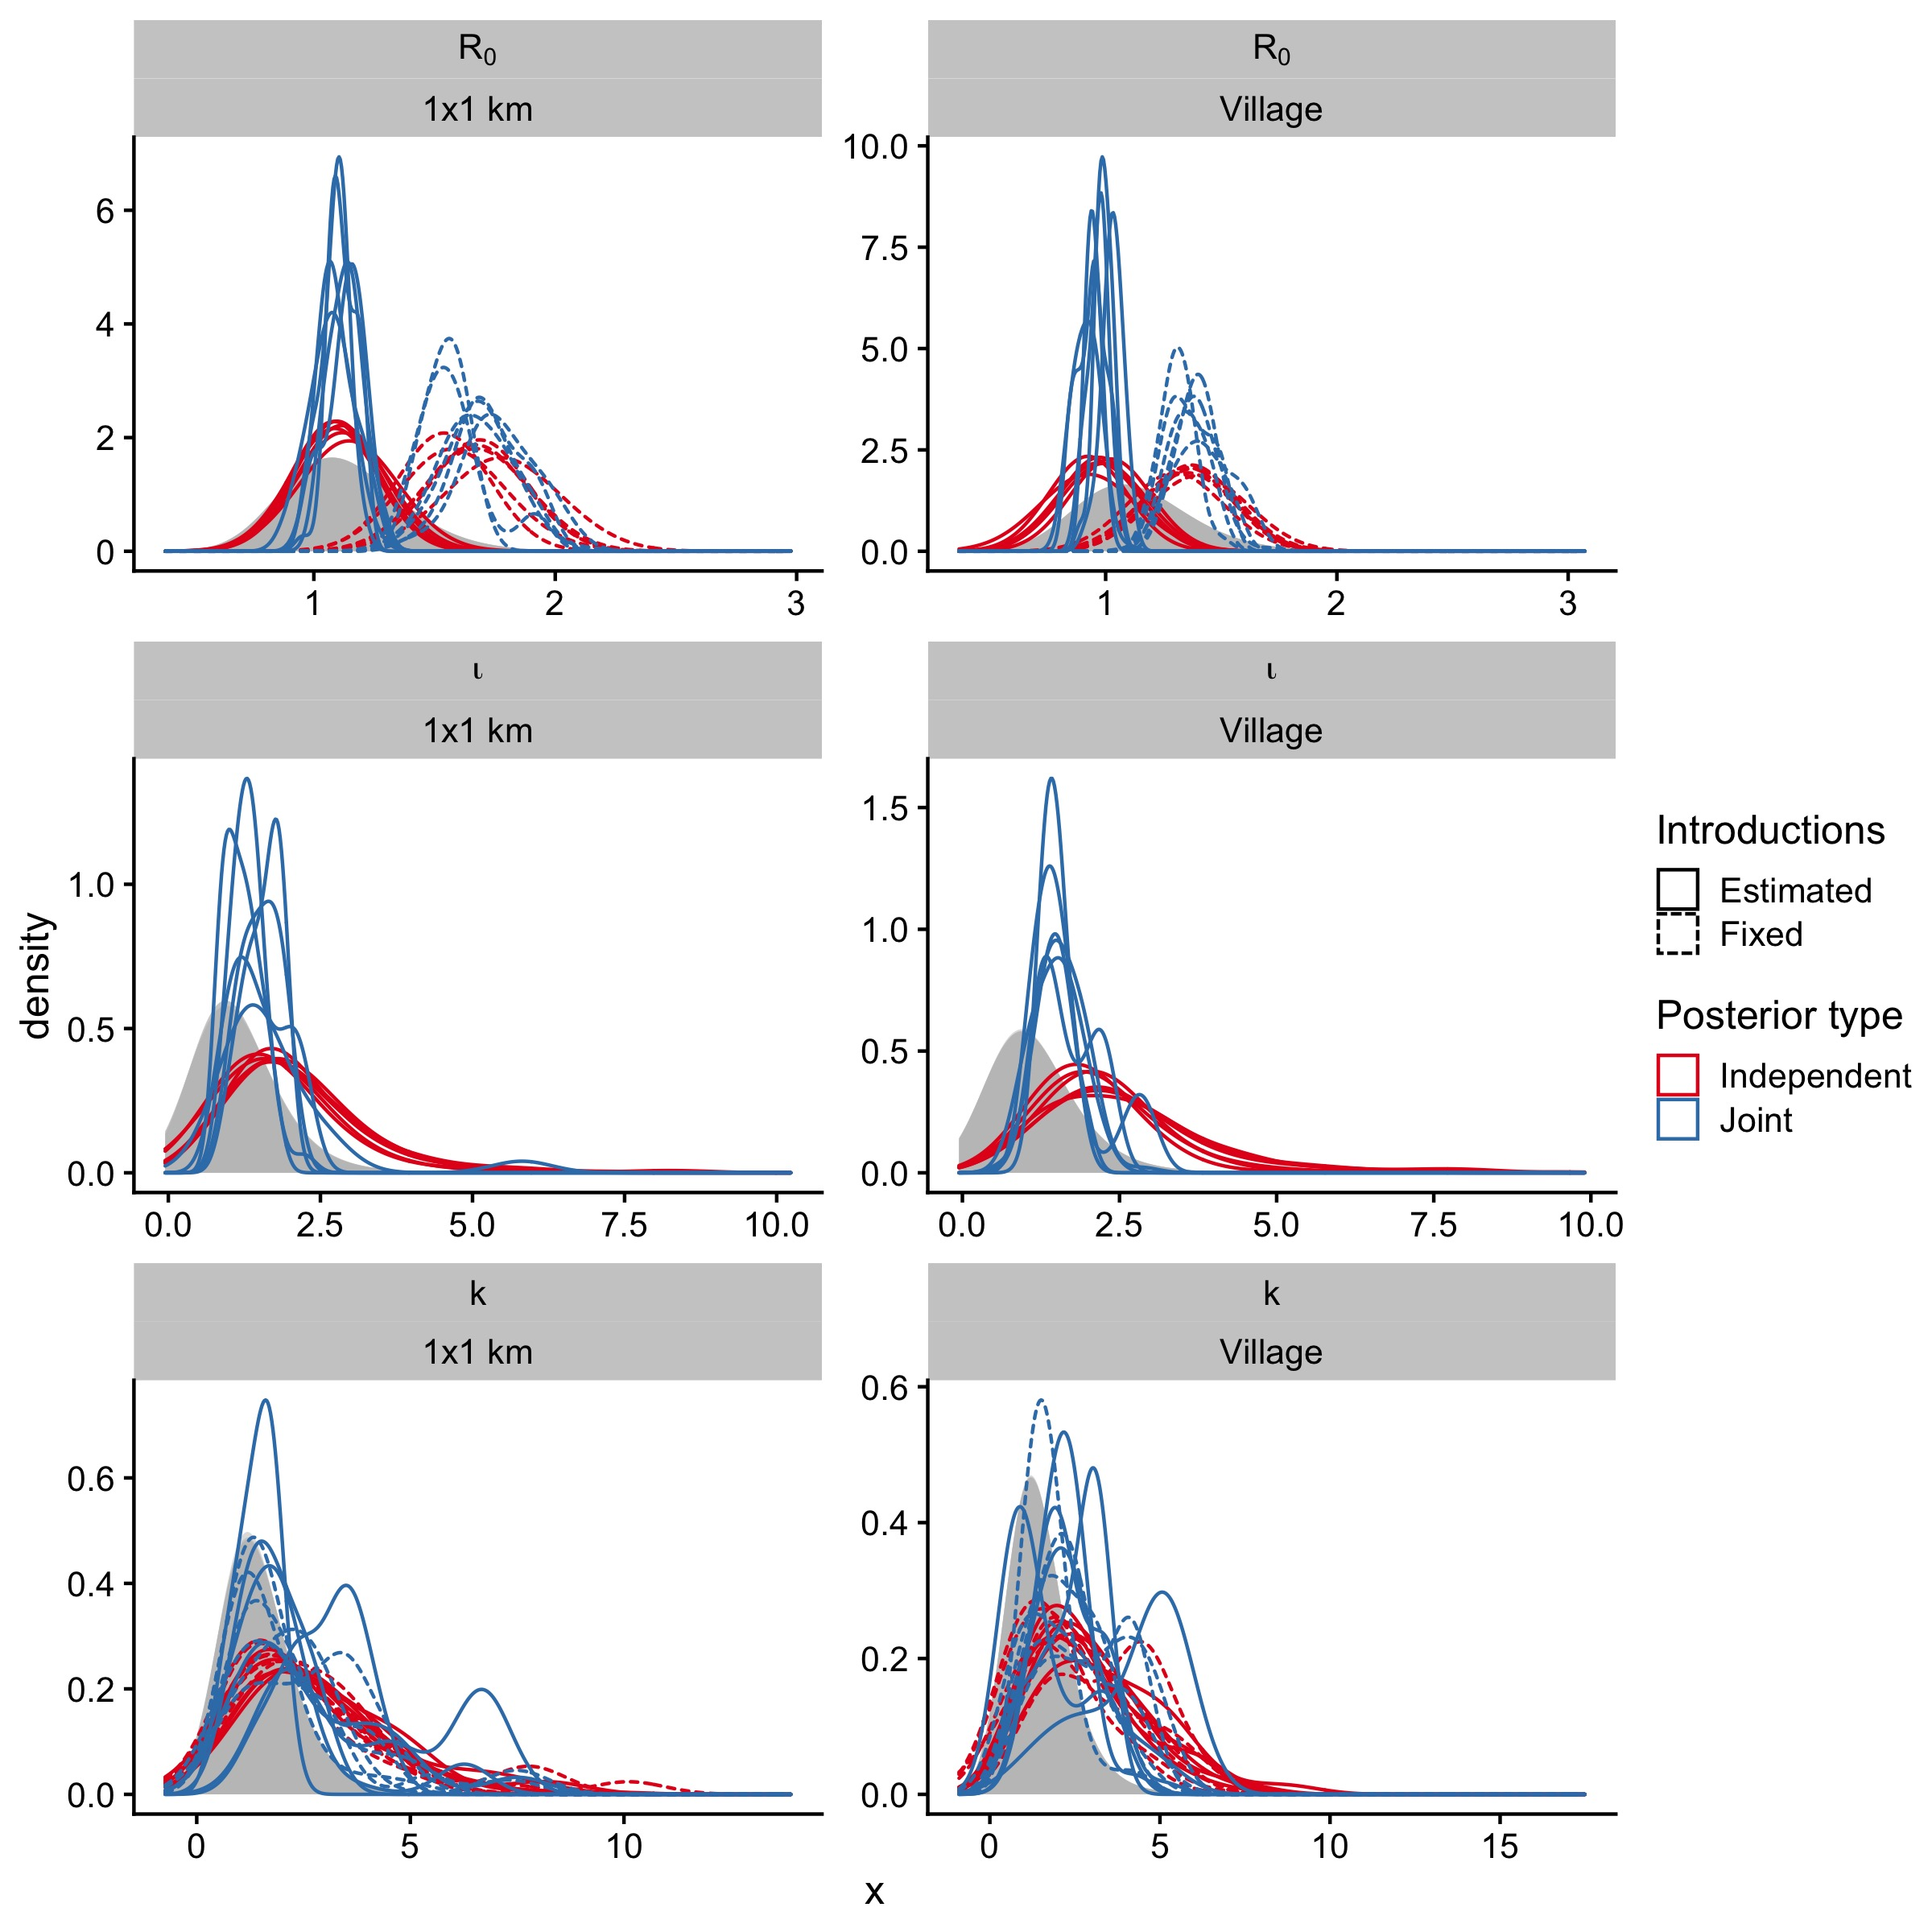
\includegraphics[width=0.9\linewidth]{/Users/mrajeev/Documents/Projects/dynamicSD/analysis/figs/sfig_posts_jntvsfull} \caption[Independent posterior estimates for models run with the full simulation data set]{Independent posterior estimates for models run with the full simulation data set (N = 1e5 simulations per model), or subsampled datasets (approx. 75\% of the full simulation data set) for each parameter and model}\label{fig:sfig-posts-jntvsfull}
\end{figure}



\begin{figure}
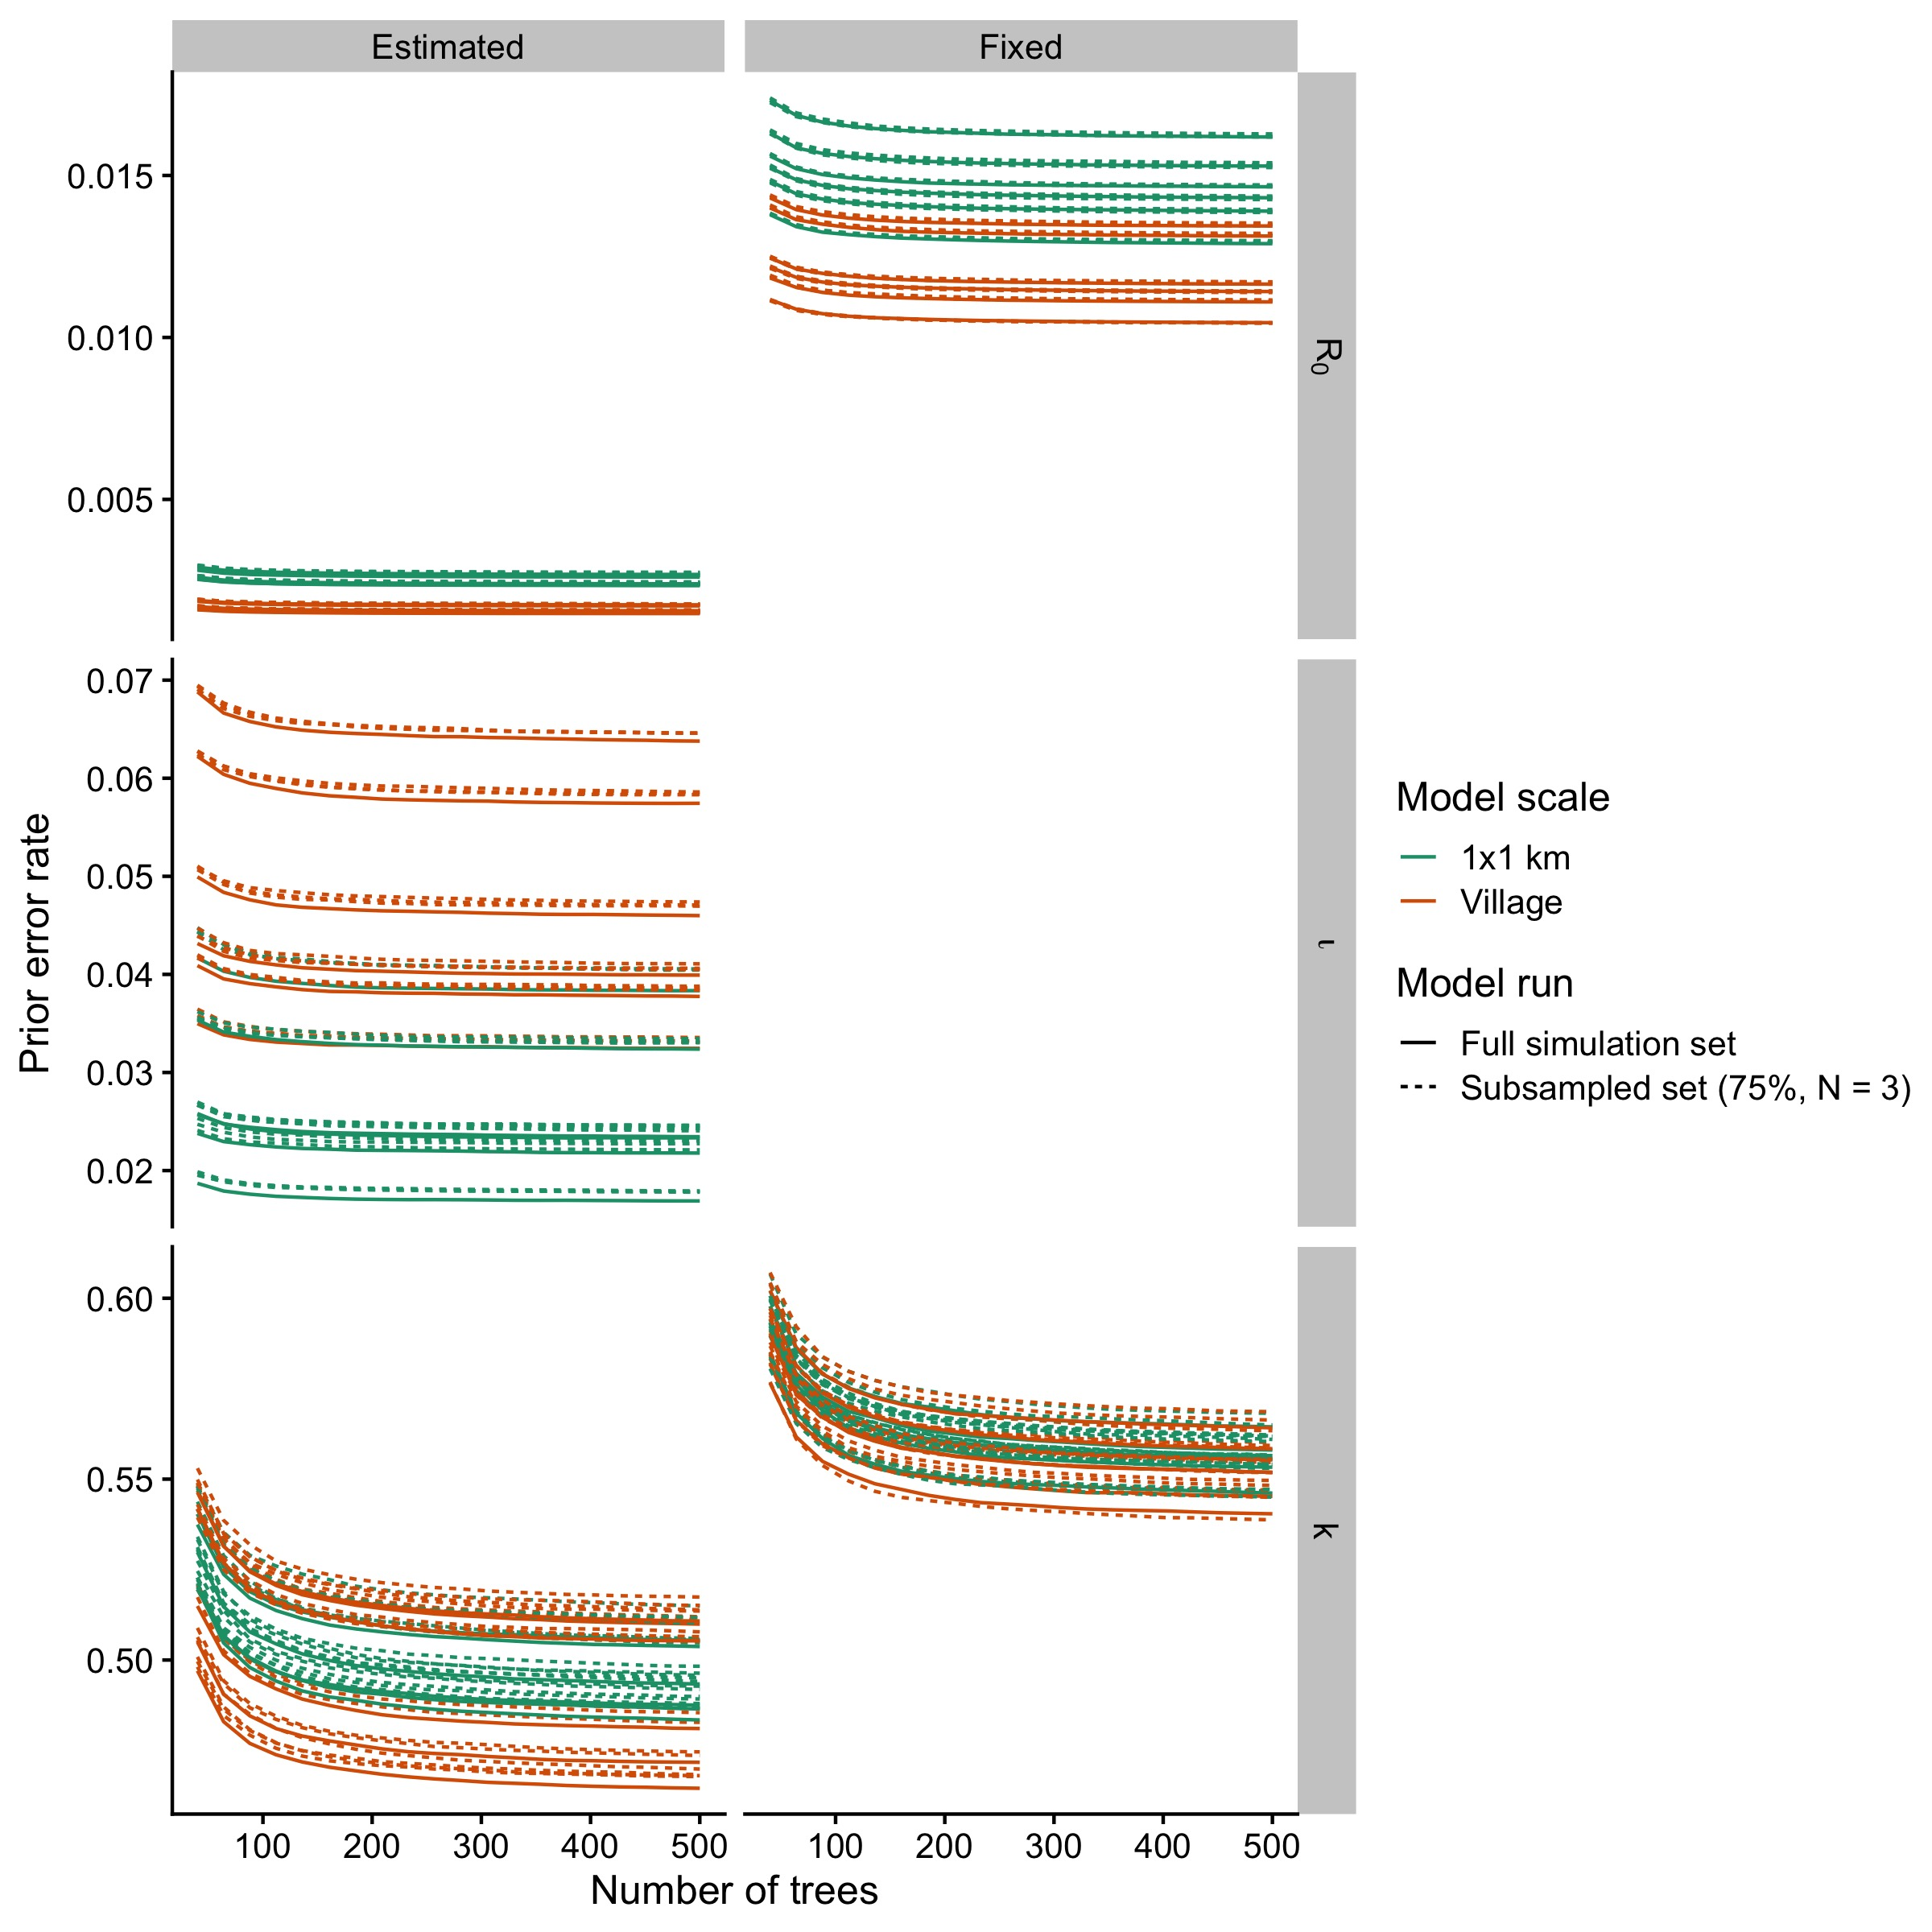
\includegraphics[width=0.9\linewidth]{/Users/mrajeev/Documents/Projects/dynamicSD/analysis/figs/sfig_posts_err} \caption{Out-of-bag error rates as trees are added separated by the scale of the model comparison and the parameter being estimated.}\label{fig:sfig-posts-err}
\end{figure}



\begin{figure}
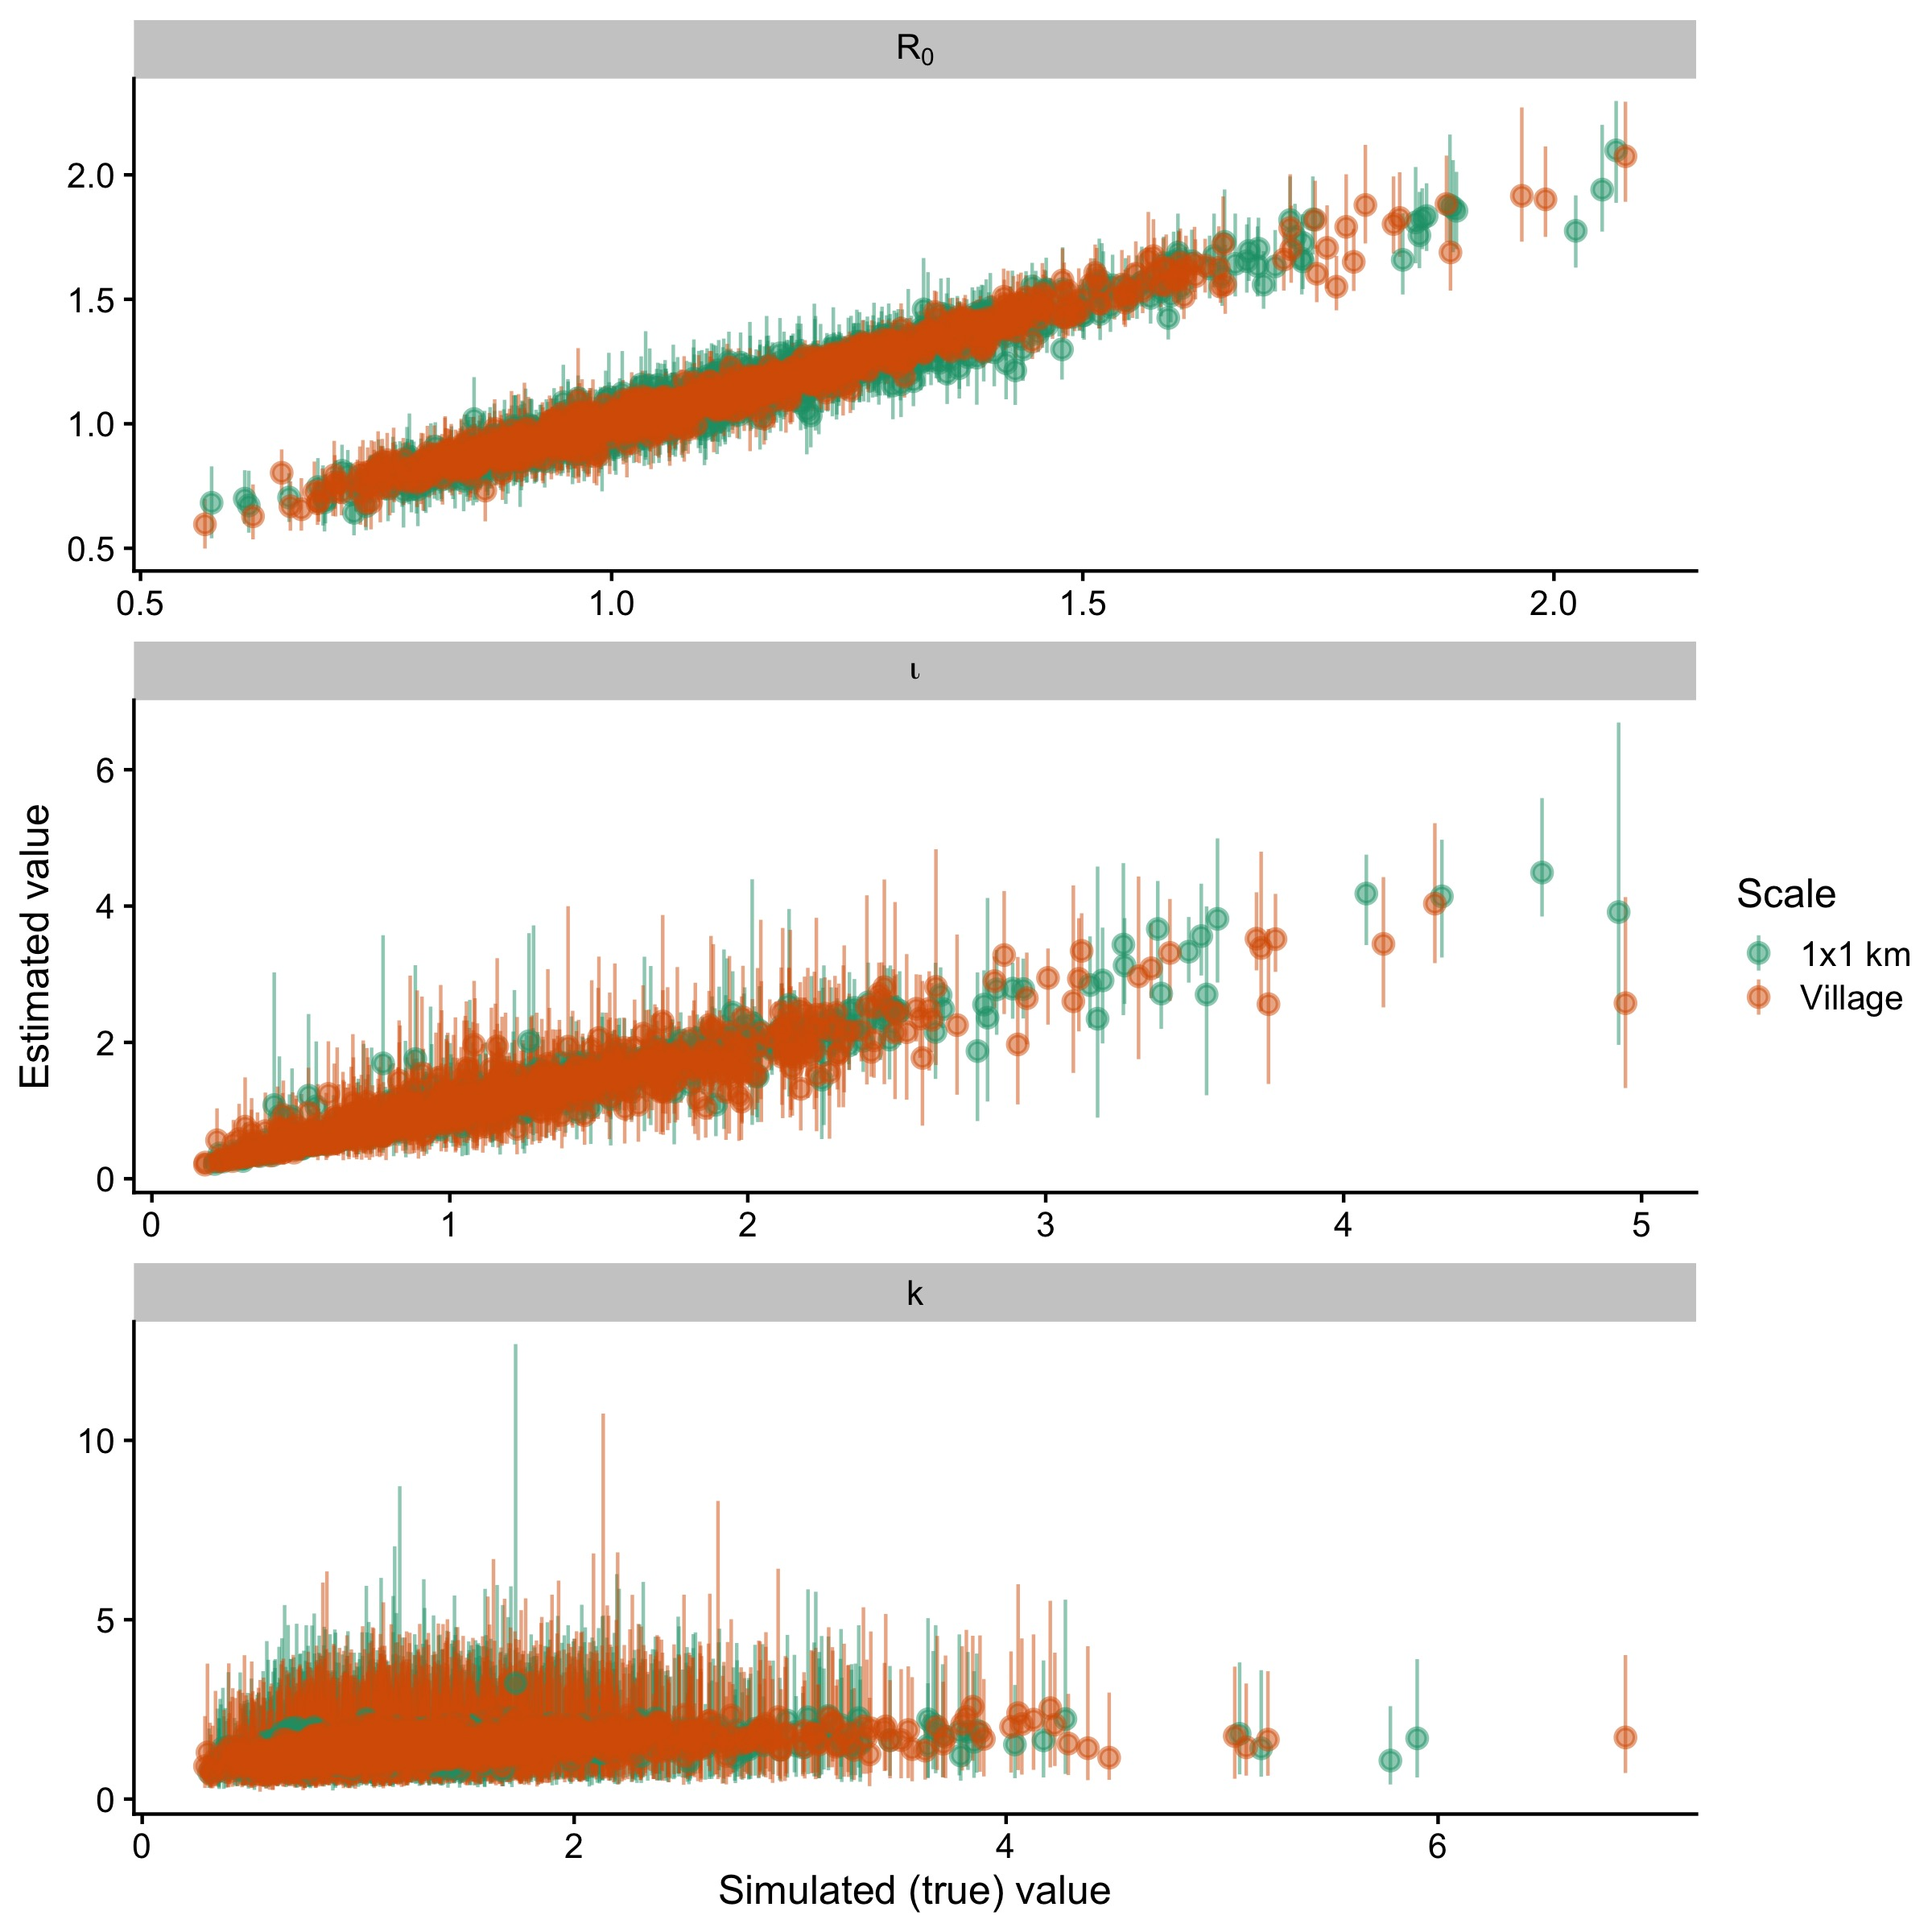
\includegraphics[width=0.9\linewidth]{/Users/mrajeev/Documents/Projects/dynamicSD/analysis/figs/sfig_param_recov} \caption{Simulated (true) parameter values vs.~model estimates for 1000 simulated datasets witheld from the classification model.}\label{fig:sfig-par-recov}
\end{figure}



\begin{figure}
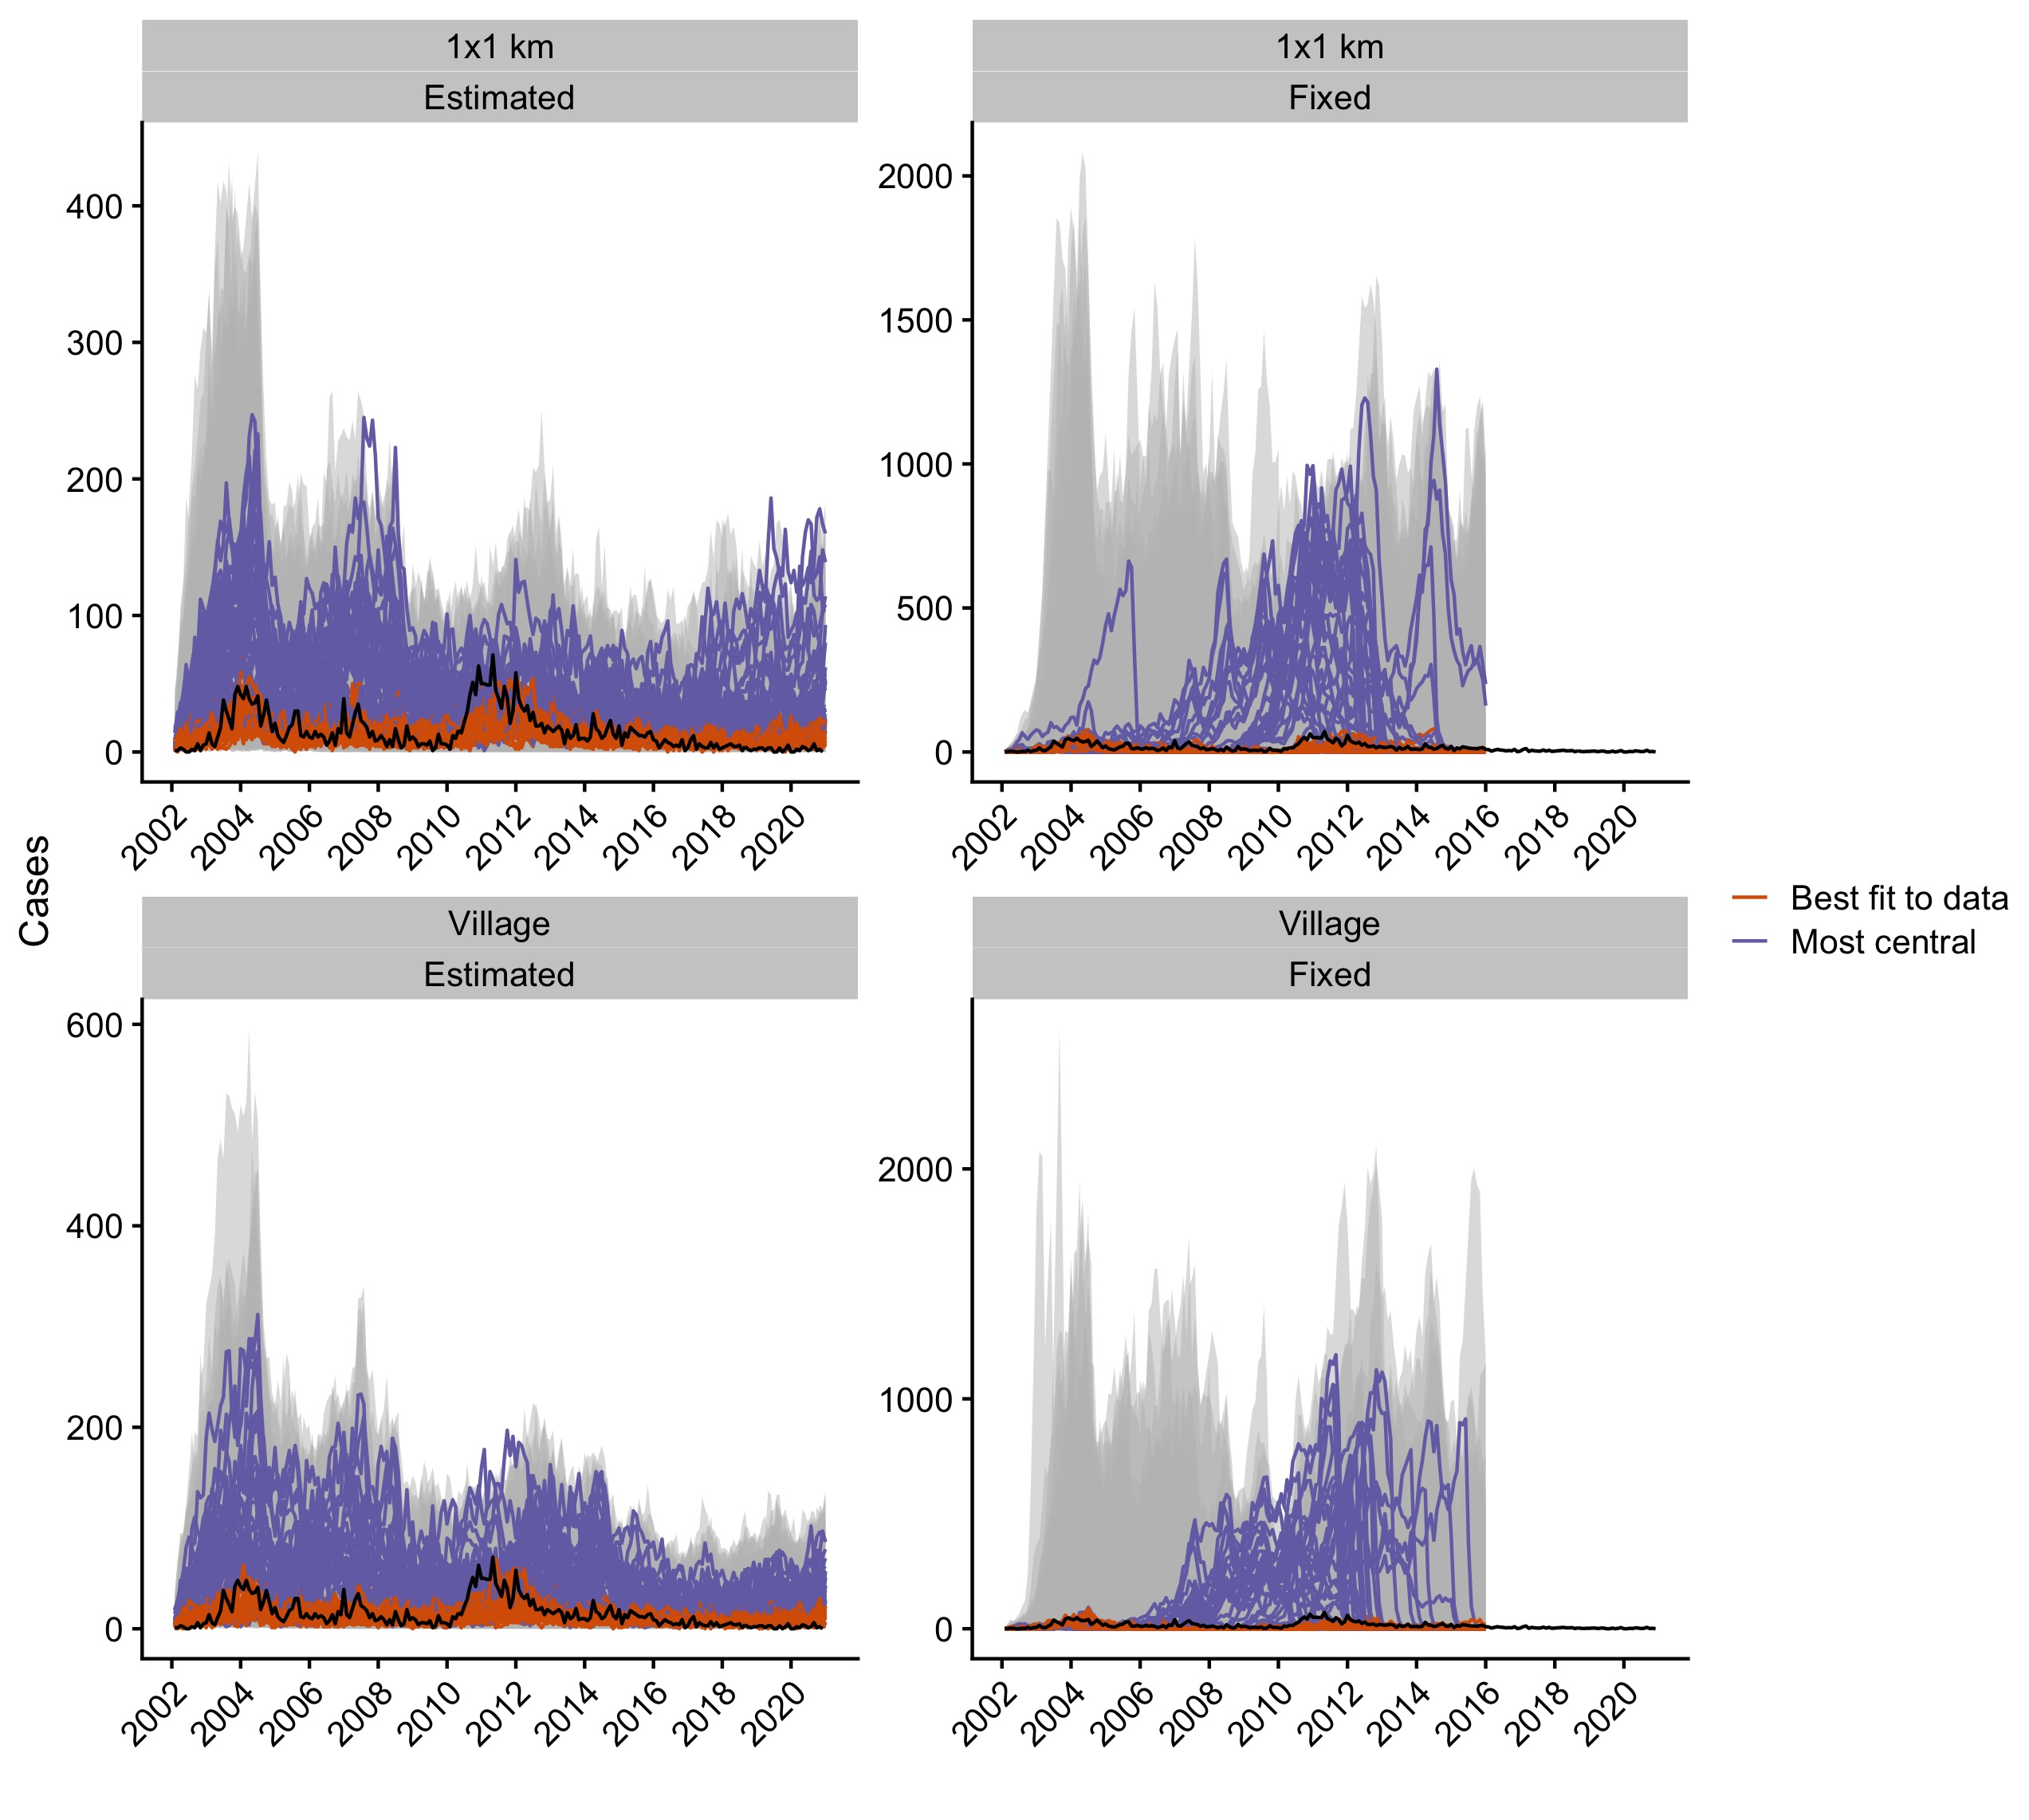
\includegraphics[width=0.9\linewidth]{/Users/mrajeev/Documents/Projects/dynamicSD/analysis/figs/sfig_sims_full} \caption[Simulations from the independent posterior estimates for all the models.]{Simulations from the independent posterior estimates for all the models. The grey envelope shows the range of simulations, and the black line is the time series of observed monthly cases. The orange lines show the top five simulations that best fit the data (lowest RMSE) and the purple lines show the top five simulations that have the highest centrality score.}\label{fig:sfig-sims-full}
\end{figure}



\begin{figure}
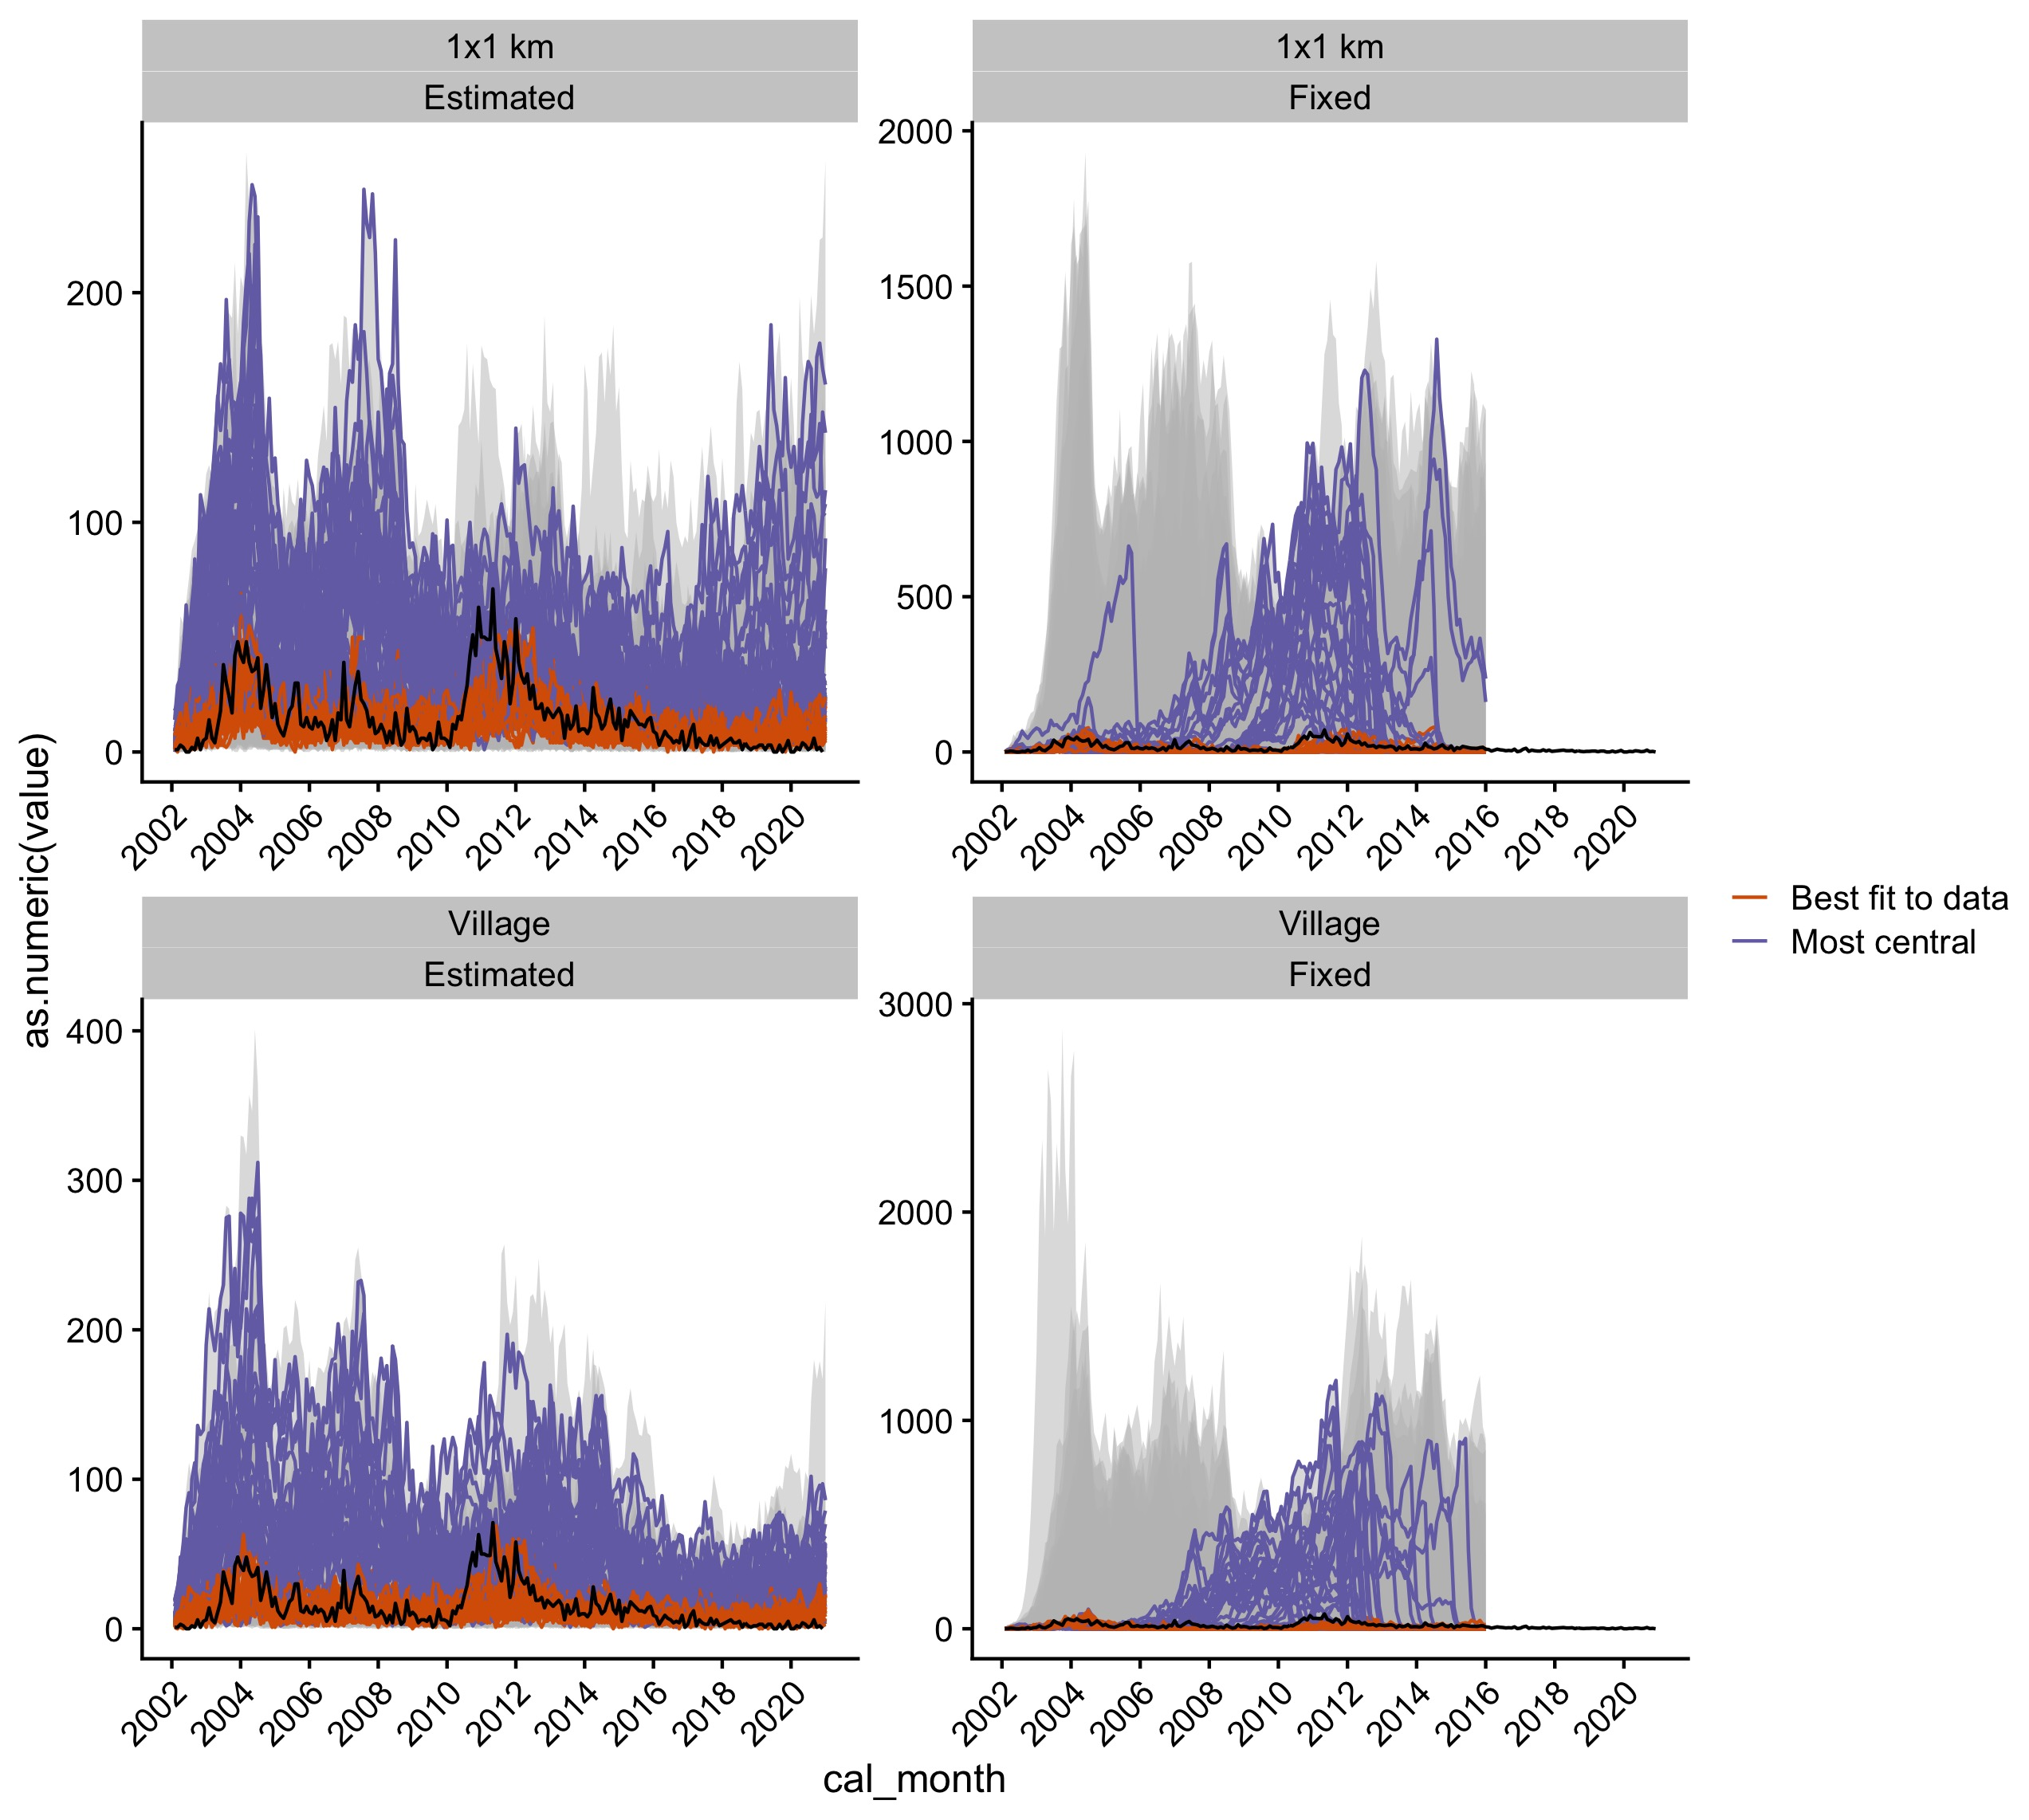
\includegraphics[width=0.9\linewidth]{/Users/mrajeev/Documents/Projects/dynamicSD/analysis/figs/sfig_sims_joint} \caption[Simulations from the joint posterior estimates for all the models.]{Simulations from the joint posterior estimates for all the models. The grey envelope shows the range of simulations, and the black line is the time series of observed monthly cases. The orange lines show the top five simulations that best fit the data (lowest RMSE) and the purple lines show the top five simulations that have the highest centrality score.}\label{fig:sfig-sims-joint}
\end{figure}



\begin{figure}
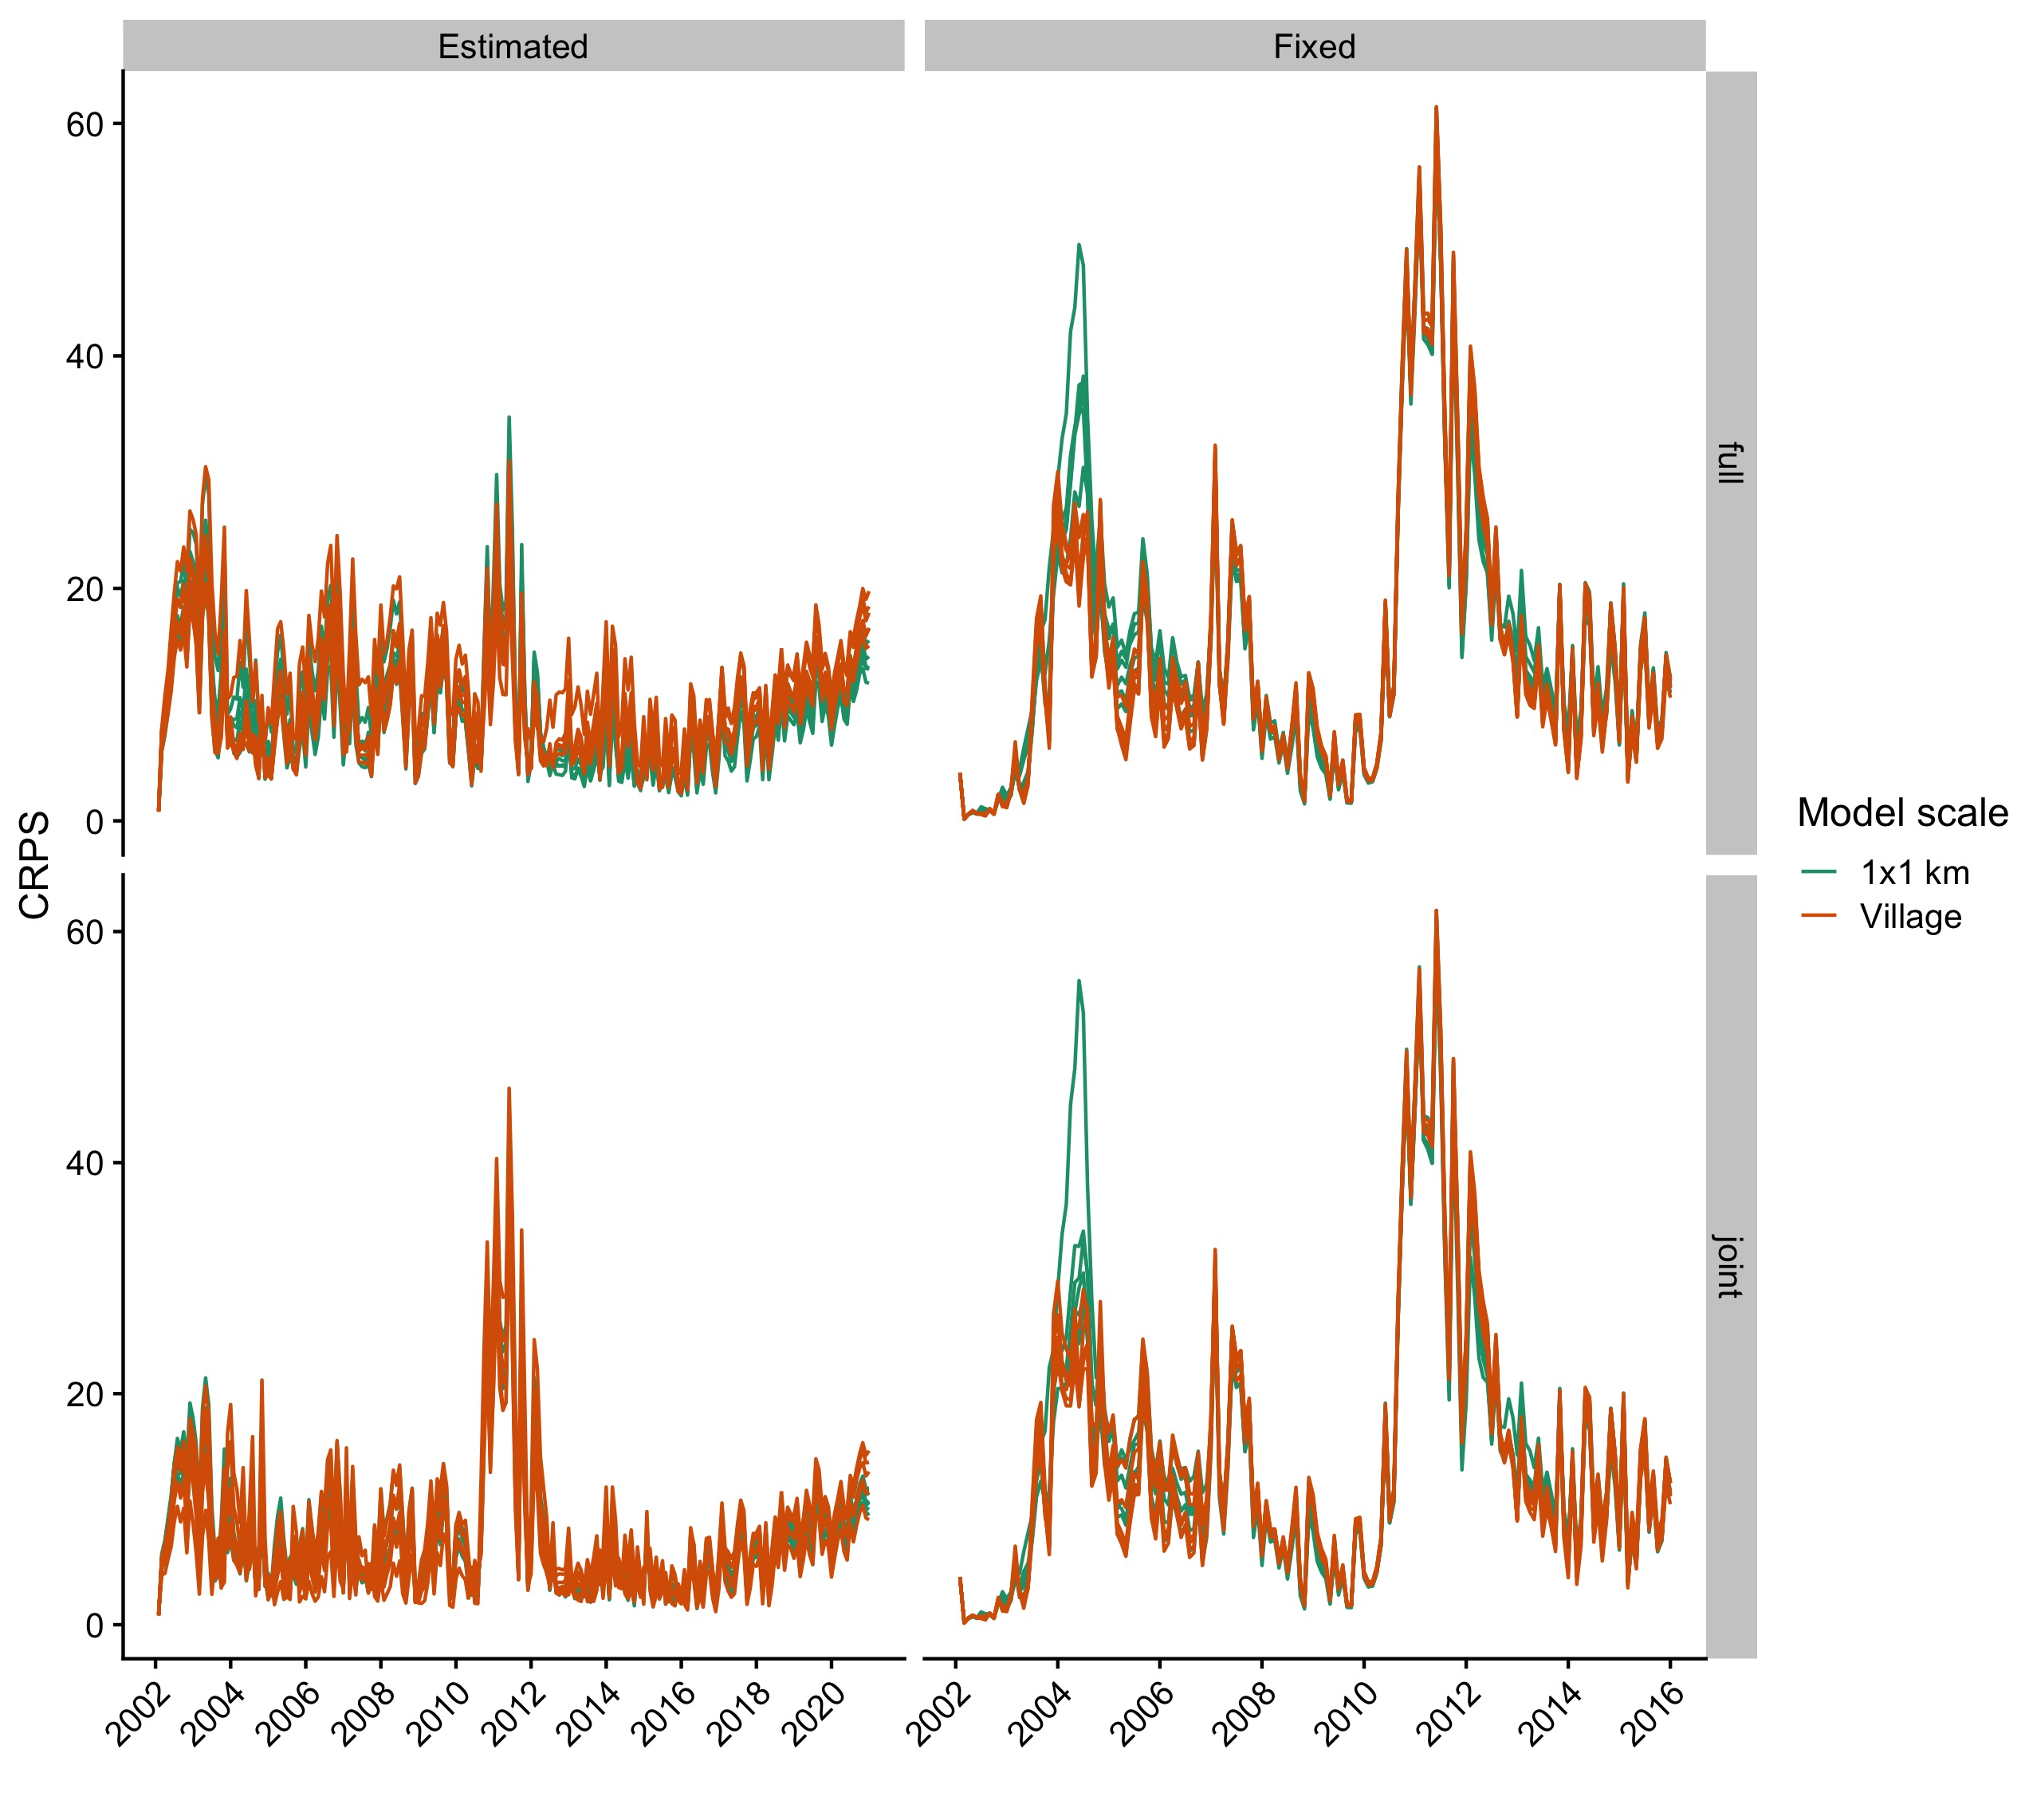
\includegraphics[width=0.9\linewidth]{/Users/mrajeev/Documents/Projects/dynamicSD/analysis/figs/sfig_sims_crps} \caption{Continuous ranked probability scores for the simulated datasets compared to the observed comparing models with estimated introduction rates (columns) and across scales (rows).}\label{fig:sfig-sims-crps}
\end{figure}



\begin{figure}
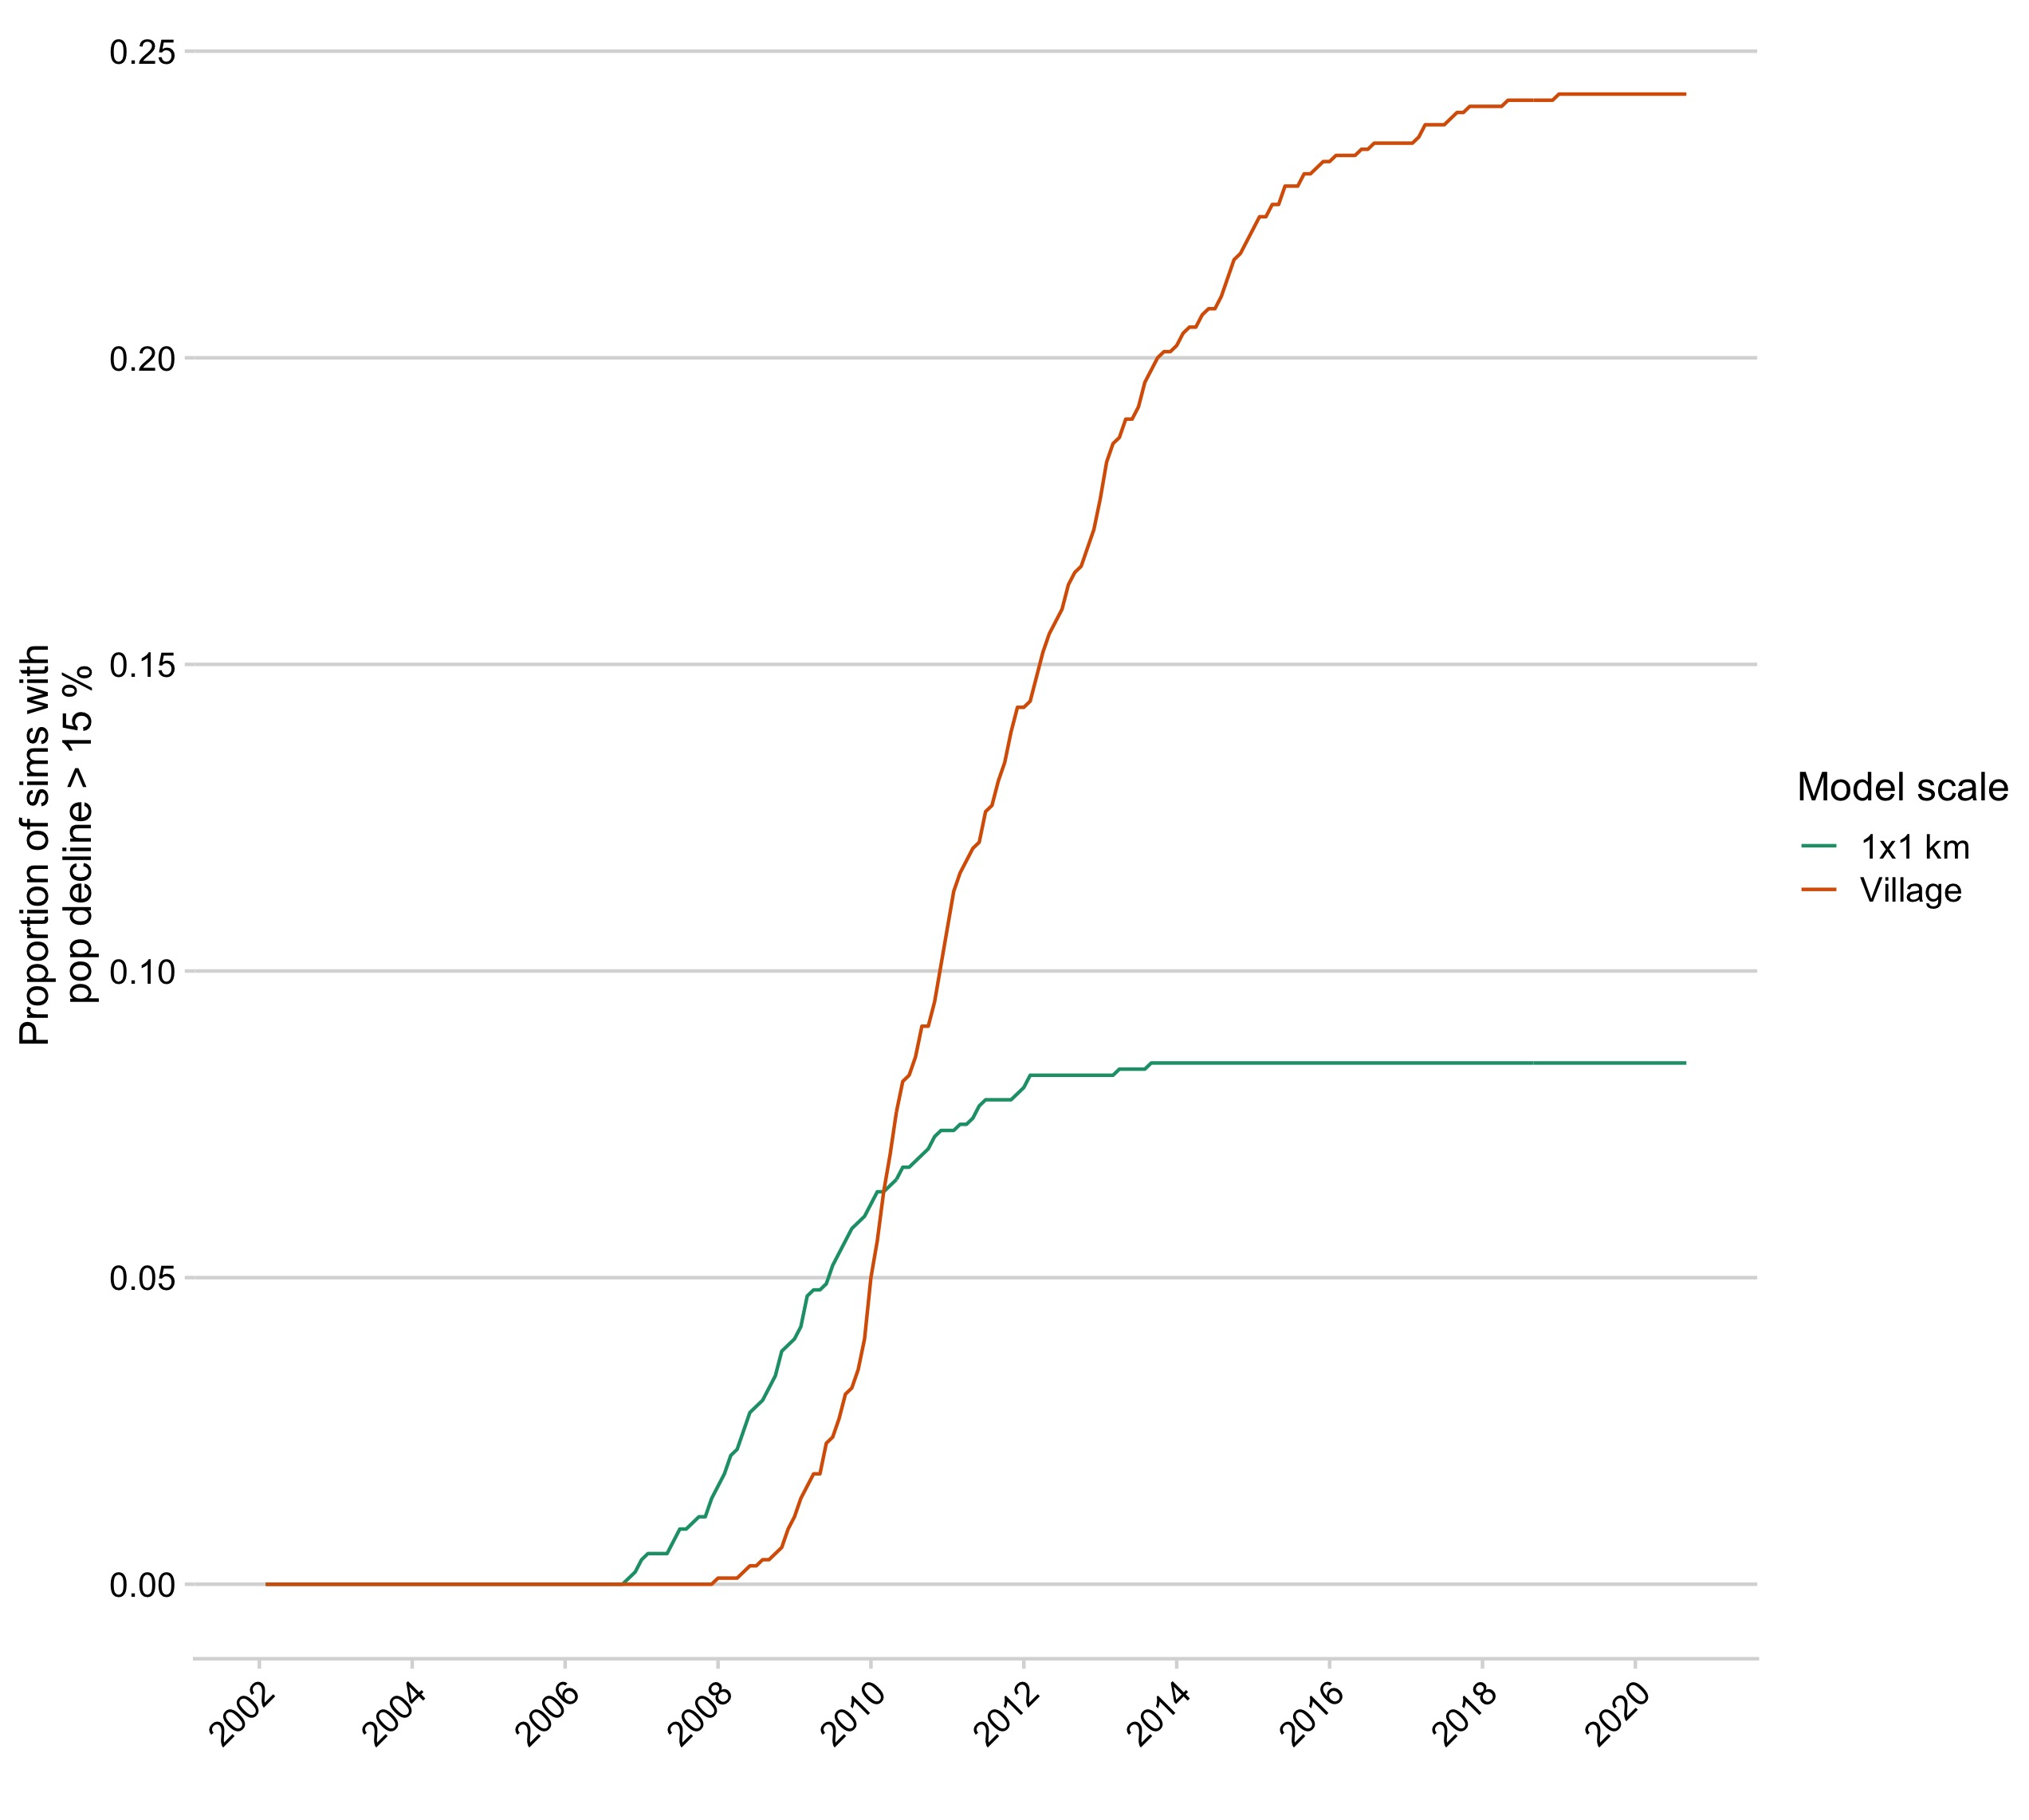
\includegraphics[width=0.9\linewidth]{/Users/mrajeev/Documents/Projects/dynamicSD/analysis/figs/sfig_sims_endemic} \caption{The proportion of simulations resulting in population declines \textgreater{} 15\% by each time step for the best model at each scale.}\label{fig:sfig-sims-endemic}
\end{figure}



\begin{figure}
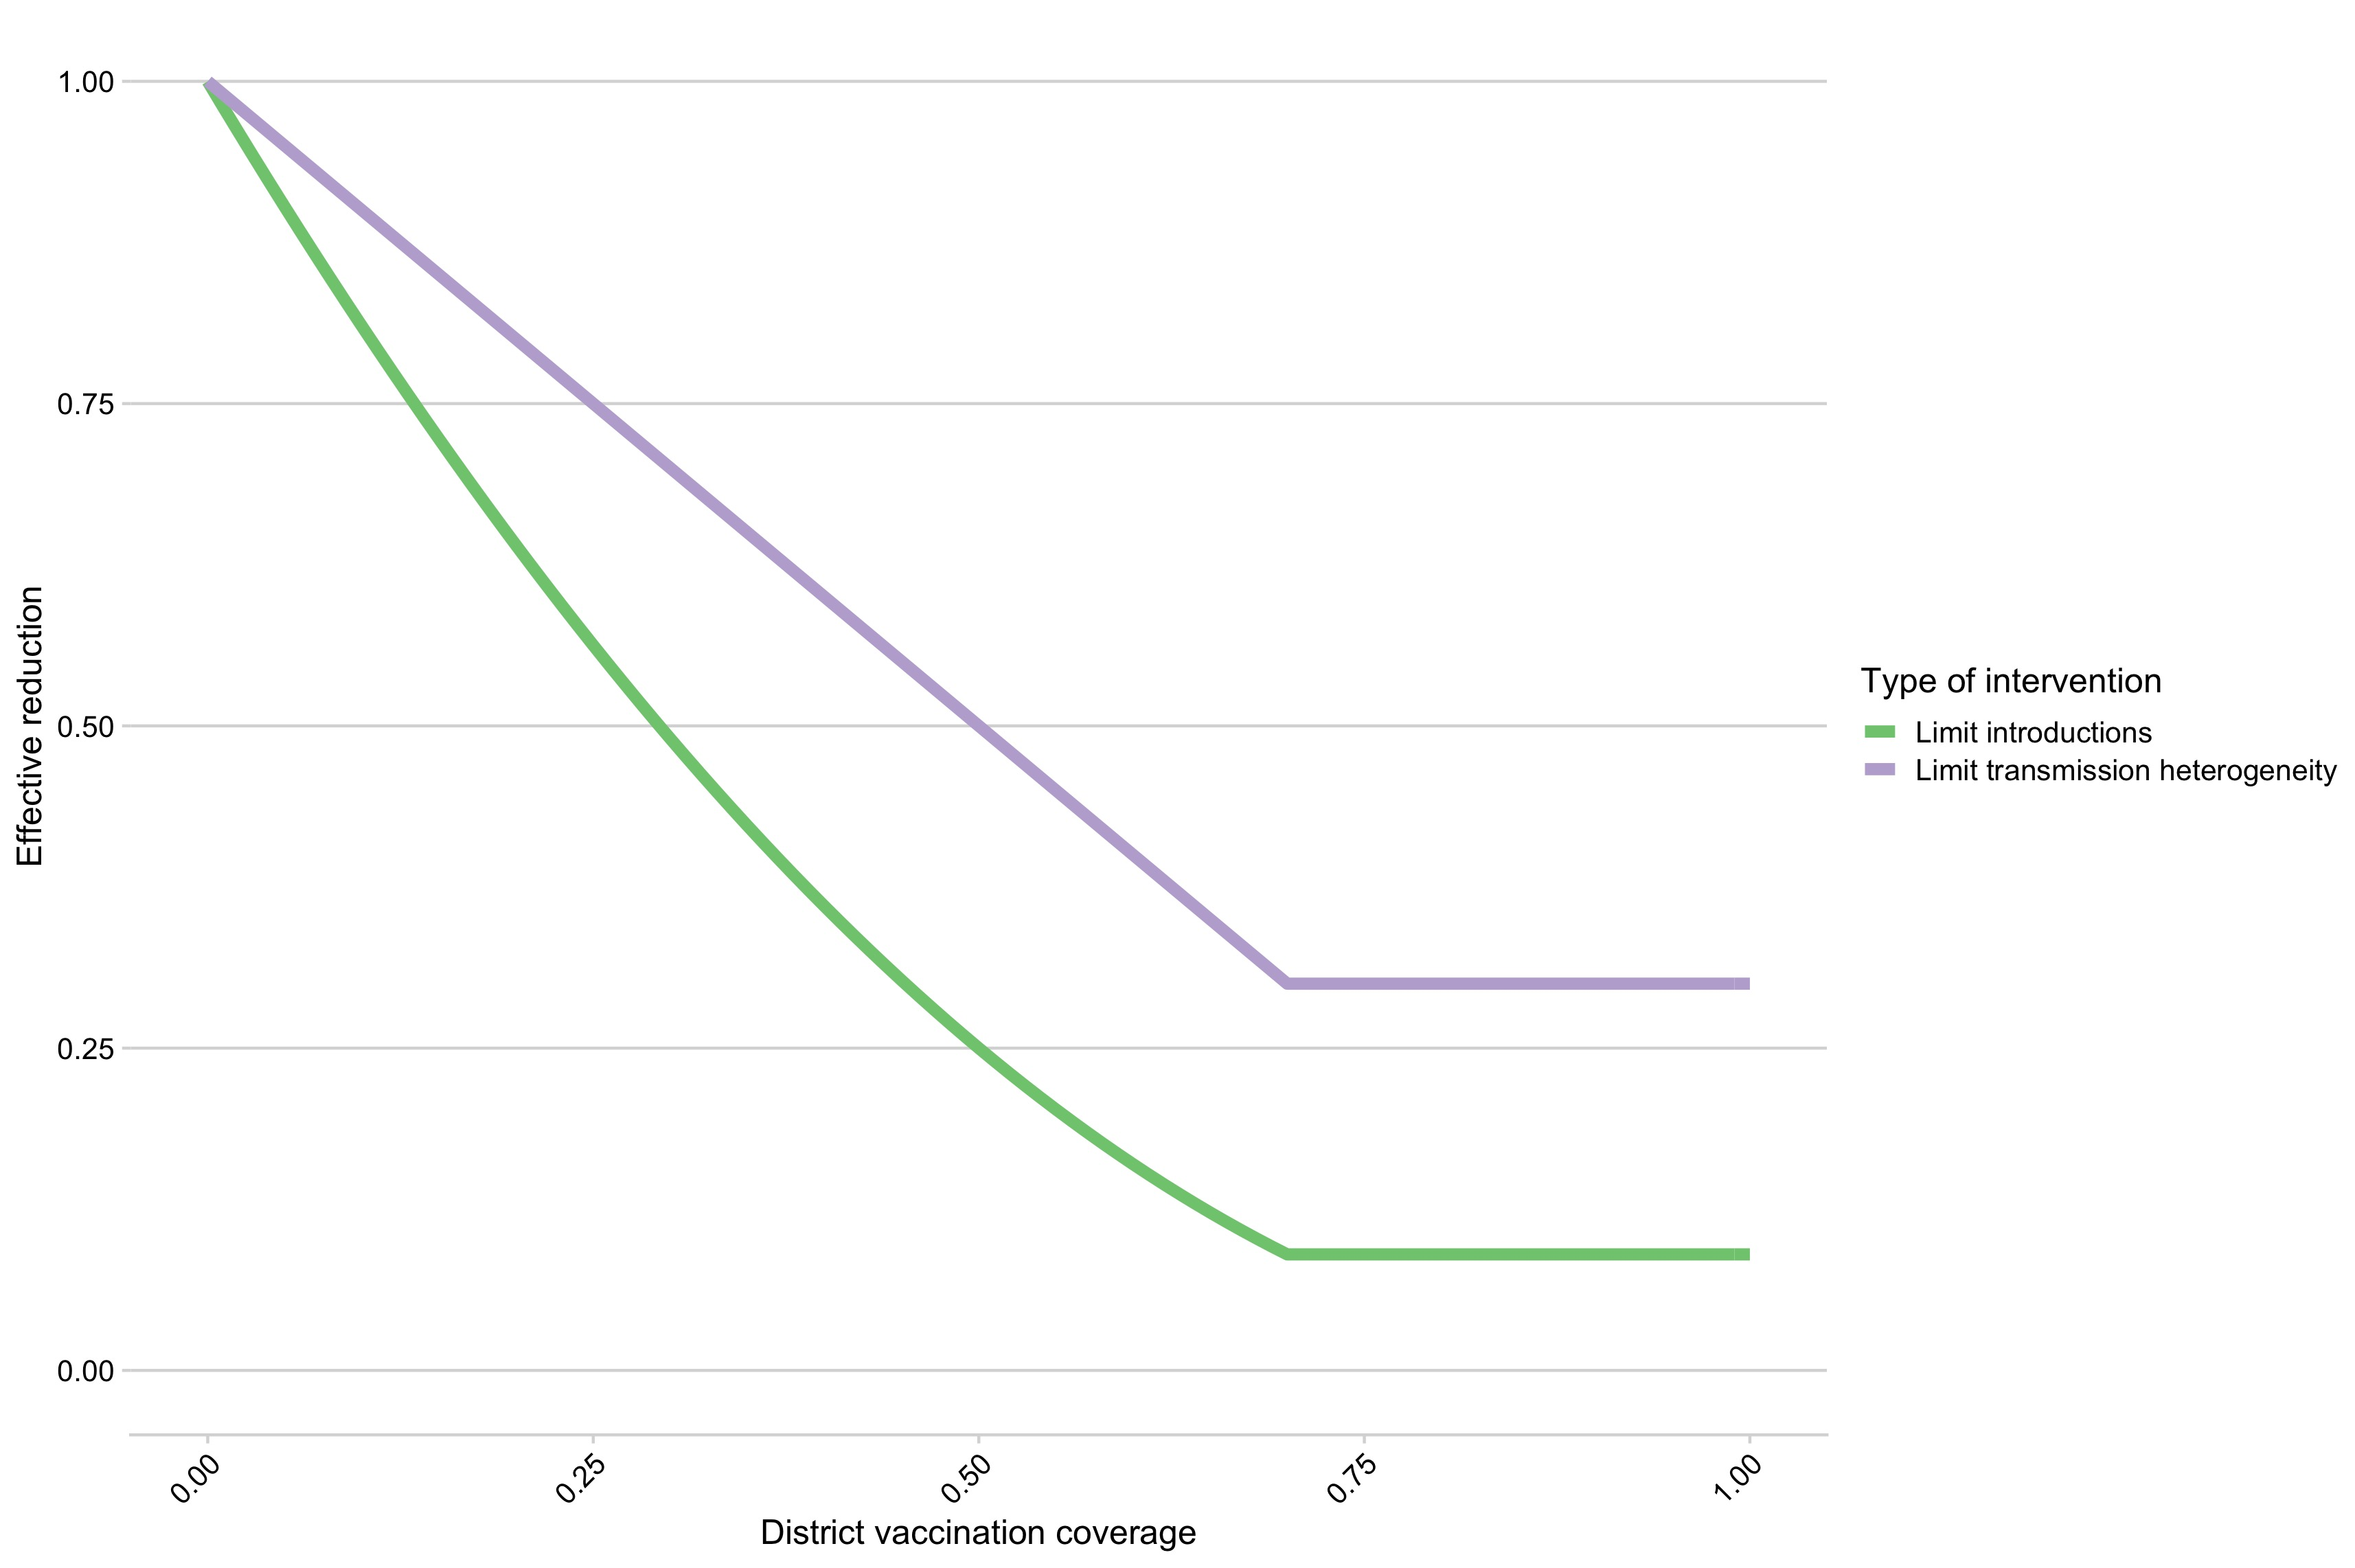
\includegraphics[width=0.9\linewidth]{/Users/mrajeev/Documents/Projects/dynamicSD/analysis/figs/sfig_conn_constraint} \caption{The relationship between district level proportion susceptible and reduction in introduction rate and limits on secondary cases.}\label{fig:sfig-conn-constraint}
\end{figure}



\begin{figure}
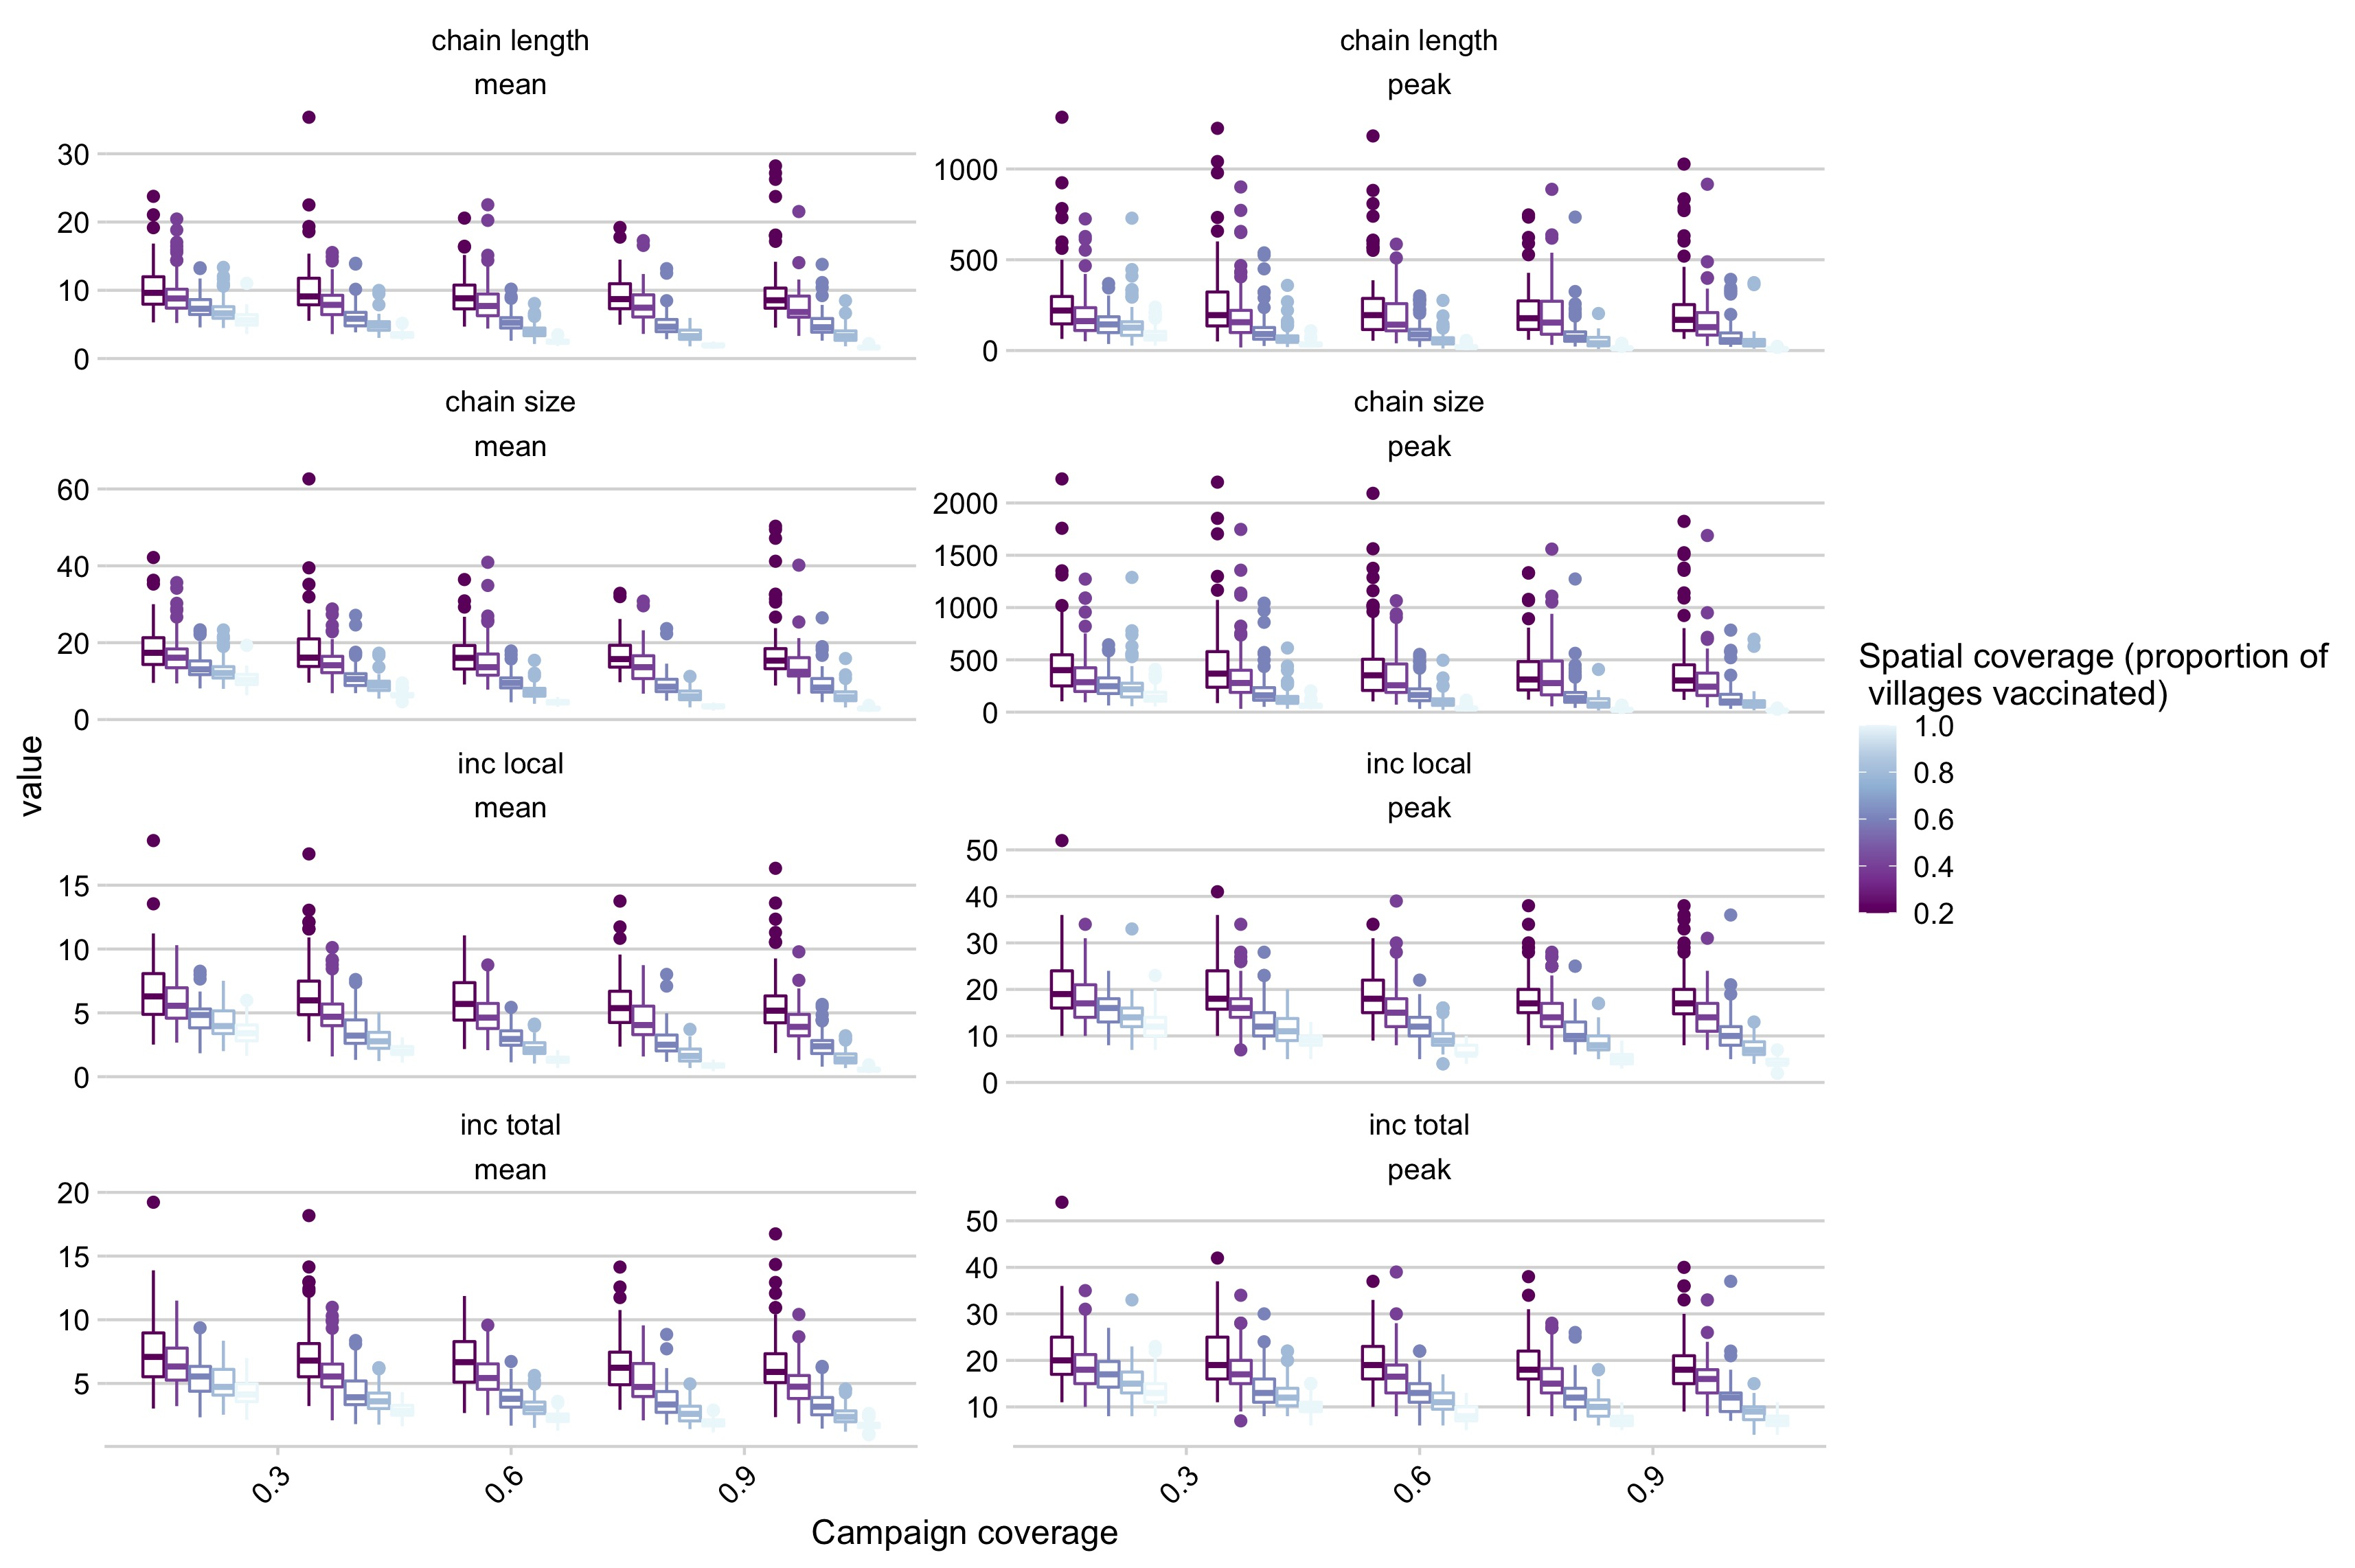
\includegraphics[width=0.9\linewidth]{/Users/mrajeev/Documents/Projects/dynamicSD/analysis/figs/sfig_base_mets} \caption{Simulation outcomes across a range of campaign coverage and spatial coverage for the baseline case where panels are different summary statistics of the simulations (i.e.~chain length mean, chain length peak, etc.).}\label{fig:sfig-base-mets}
\end{figure}



\begin{figure}
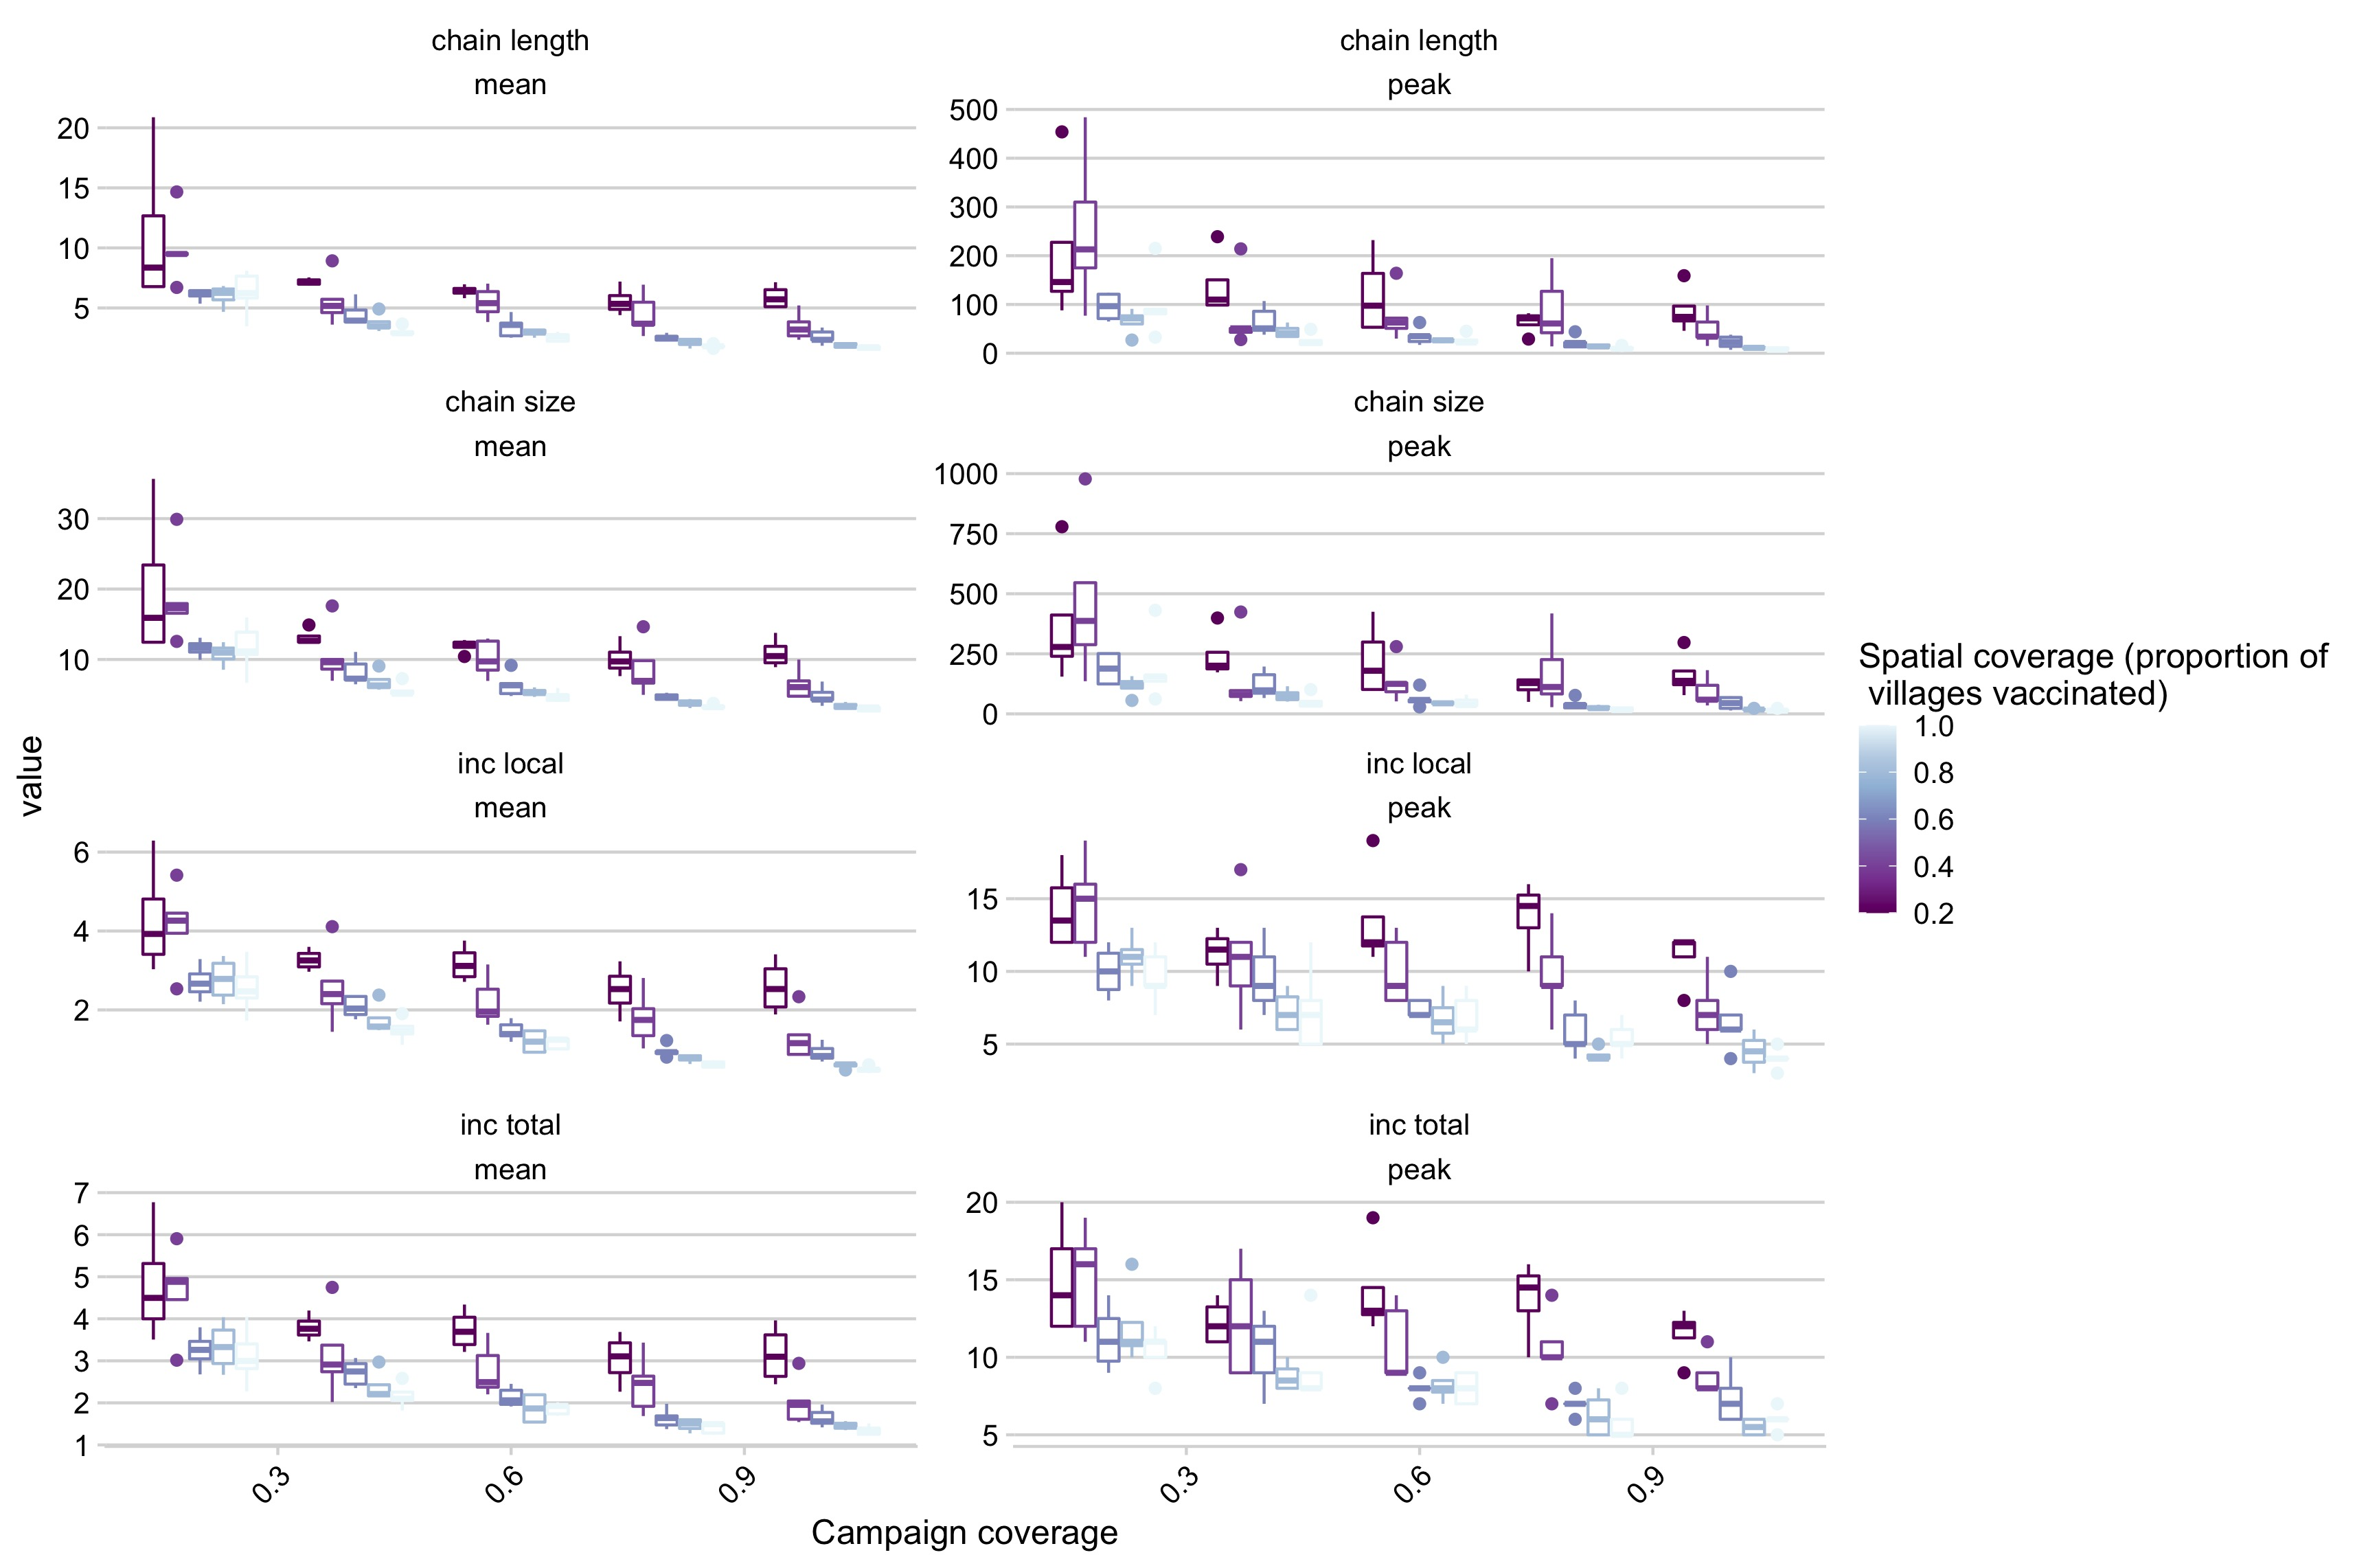
\includegraphics[width=0.9\linewidth]{/Users/mrajeev/Documents/Projects/dynamicSD/analysis/figs/sfig_sspread_mets} \caption[Simulation outcomes across a range of campaign coverage and spatial coverage.]{Simulation outcomes across a range of campaign coverage and spatial coverage incorporating reductions in the maximum number of secondary cases rate as district coverage increases where panels are different summary statistics of the simulations (i.e.~chain length mean, chain length peak, etc.).}\label{fig:sfig-sspread-mets}
\end{figure}



\begin{figure}
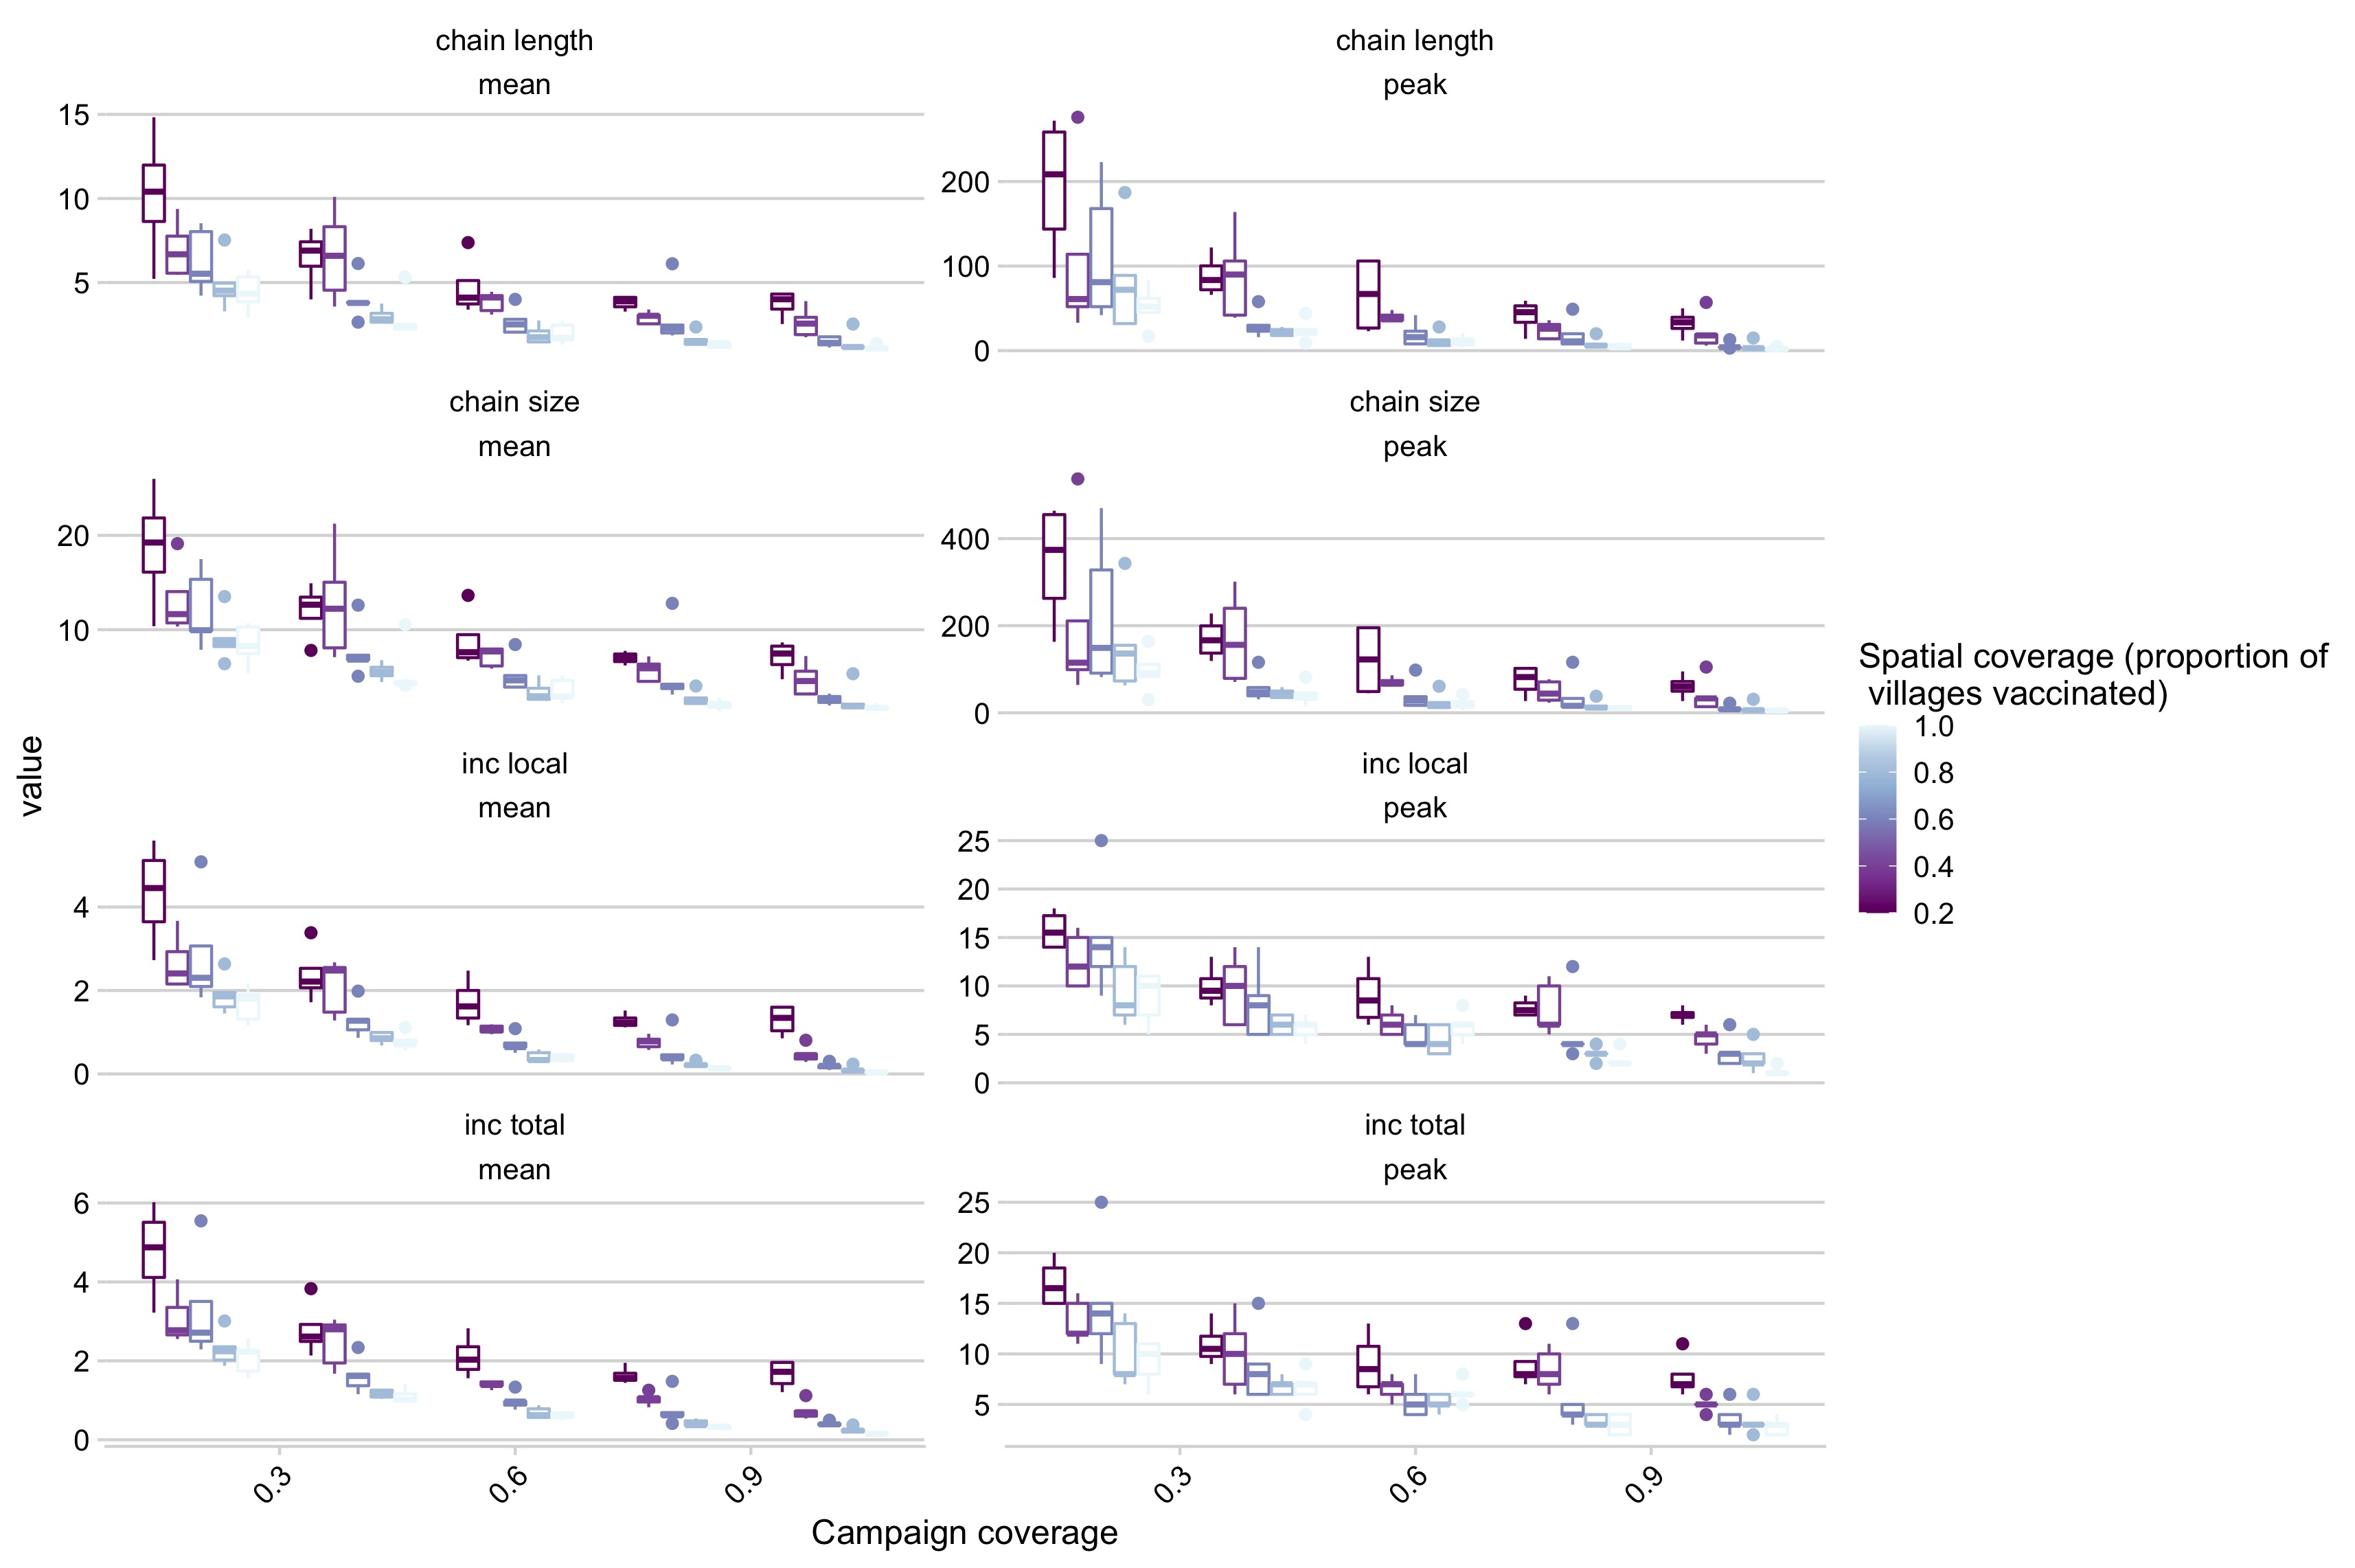
\includegraphics[width=0.9\linewidth]{/Users/mrajeev/Documents/Projects/dynamicSD/analysis/figs/sfig_incs_mets} \caption{Simulation outcomes across a range of campaign coverage and spatial coverage incorporating reductions in the introduction rate as district coverage increases where panels are different summary statistics of the simulations (i.e.~chain length mean, chain length peak, etc.).}\label{fig:sfig-incs-mets}
\end{figure}



\begin{figure}
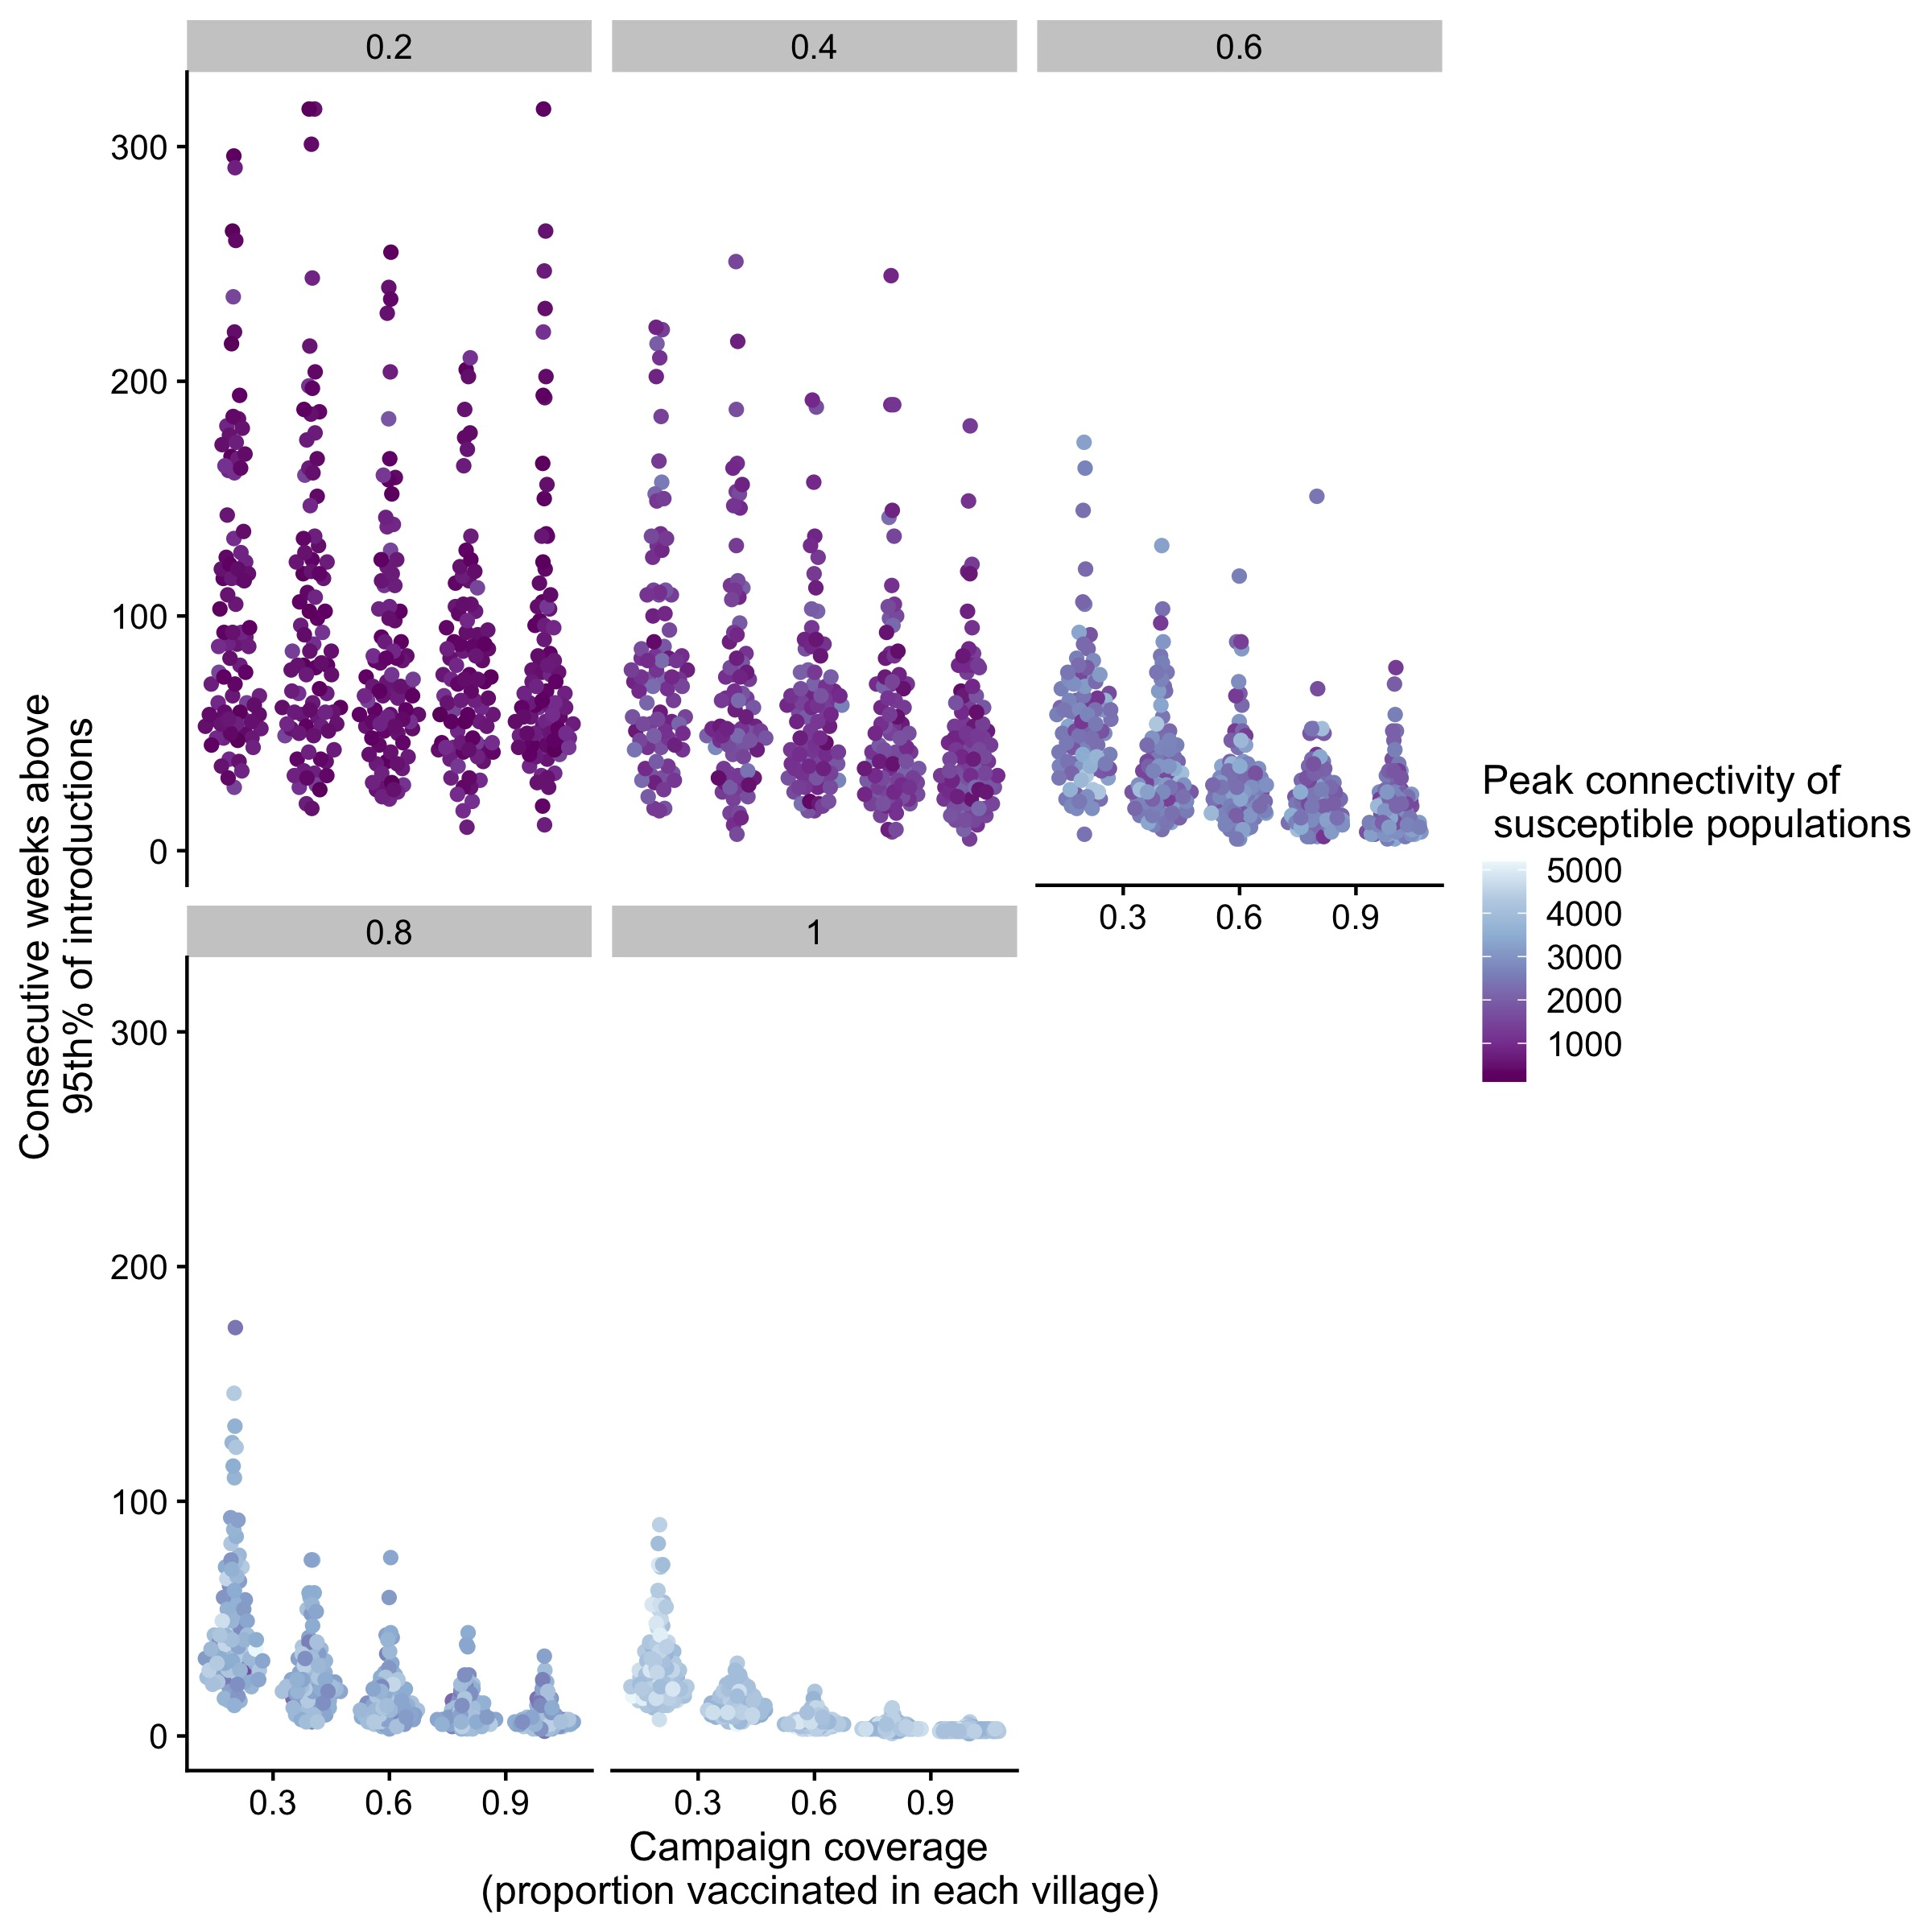
\includegraphics[width=0.9\linewidth]{/Users/mrajeev/Documents/Projects/dynamicSD/analysis/figs/sfig_conn_mets} \caption{Outbreak durations (weeks with cases \textgreater{} 95th \% of introductions) and their relationship to connectivity of villages across a range of campaign coverages (i.e.~proportion vaccinated in each village, x-axis) and spatial coverage (proportion of villages vaccinated, panels).}\label{fig:sfig-conn-mets}
\end{figure}



\hypertarget{conclusion-1}{%
\chapter{Conclusion}\label{conclusion-1}}

\setlength{\parskip}{2em}

My dissertation focuses on integrating data and models with an informed understanding of pathogen biology and ecology to inform the control and elimination of canine rabies. In Chapter 2, I established a surveillance study of canine rabies in the Moramanga District, Madagascar to evaluate surveillance and burden of rabies. I find that poor surveillance masks high burden of human deaths and exposures and the continuous endemic circulation of canine rabies. The clinic-based investigation tools developed in this study could be usefully applied at a larger scale and in more settings to improve surveillance. In Chapter 3, I integrate this finer scale, comprehensive data, with broader scale, messy routine public health data, and develop statistical models that can integrate these data across scales to estimate the impact of geographic access to PEP on shaping rabies burden in Madagascar, and how expanding access to PEP can reduce this burden. I find that even given ideal expansion of PEP to all major health centers in Madagascar, that a substantial number of deaths will still occur due to the landscape of care. This work also highlights how using data naively without considering its biases in representation can skew estimates of burden and outcomes. I use two case studies to highlight that while access to this life-saving vaccine should be a matter of equity, that predicting human behavior and care seeking is challenging and that even in best case scenarios PEP alone will like not be able to eliminate deaths due to canine rabies.

In Chapter 4, I review the existing body of mathematical modeling studies for canine rabies, and point out key gaps both methodologically and in terms of data. I find that existing models of canine rabies generally fail to capture endemic and epidemic disease dynamics, and that few modeling studies use data to fit their models, largely due to the lack of high quality routine surveillance data available. Finally in Chapter 5, I work to address these gaps by using simulation-based inference to fit individual-based model to a rich dataset on canine rabies cases and domestic dog populations in the Serengeti District, Tanzania. I find that integrating both the spatial scale of control and of population mixing is key to predicting observed dynamics and expectations of endemic diseases. Incorporating this understanding into strategies for control, i.e.~focusing on spatial as well as temporal coverage targets or coordinating vaccination or surveillance efforts across larger geographic scales, could improve control prospects.

\hypertarget{future-directions}{%
\section{Future directions}\label{future-directions}}

Overall, my work highlights how integrating models and data can allow us to bound our expectations for transmission and disease outcomes. Moving forward methodologically in terms of dynamic modeling of canine rabies, integrating other data streams such as phylogenetic data into epidemiological models could shed light on the scale of maintenance for canine rabies \protect\hyperlink{ref-bourhy2016}{{[}52{]}}, \protect\hyperlink{ref-brunker2018}{{[}56{]}}, \protect\hyperlink{ref-dellicour2017}{{[}57{]}}. Further work is needed to explore the impact that larger scale spatial and landscape structure may have on canine rabies dynamics. While the individual based model I developed was simplified to implicitly capture many aspects of rabies transmission, this modeling and inference framework relies on high resolution population and case data. Ultimately, developing approximations for key aspects of transmission that can be captured implicitly (such as the scale of mixing) without needing explicit data to parameterize them, could be key to adoption of improved modeling frameworks that align with observed dynamics. More broadly, this work mirrors many of the pressing issues facing infectious disease modelers: 1) How do we balance complexity and tractability of models; 2) How do we integrate noisy and incomplete data into quantitative modeling approaches and quantify the uncertainty appropriately; 3) How do we use statistical methods to make inferences from these imperfect models and data \protect\hyperlink{ref-funk2020}{{[}16{]}}, \protect\hyperlink{ref-park2020}{{[}17{]}}. This work also highlights emergent issues in control and elimination, such as the importance of social and spatial heterogeneities in vaccination coverage \protect\hyperlink{ref-takahashi2017}{{[}58{]}}, the development of improved coverage targets based on the disease specific context \protect\hyperlink{ref-funk2019}{{[}59{]}}, and the role of connectivity in promoting persistence of infectious diseases across large scales {[}\protect\hyperlink{ref-kraemer2018}{{[}60{]}}.

\hypertarget{policy-reccommendations}{%
\section{Policy Reccommendations}\label{policy-reccommendations}}

Overall, my work contributes many practical recommendations to how to improve rabies surveillance and control programs. In addition to the work presented here, the field work in Madagascar resulted in two other policy relevant outputs: 1) a comparison of filter paper as a diagnostic tool to increase sampling in remote areas and 2) a comparison of pilot vaccination campaigns and modeling of alternative community based vaccination strategies in the Moramanga District (see Appendix for full abstracts). These studies point to the importance of accounting for the context specific challenges, which in Madagascar are largely inequalities spatially in access to care and services. The work in Chapter 3 builds on this knowledge and develops new methods for analyzing bite patient data that attempt to account for who is not represented in this data. This approach could be applied to other settings to prioritize areas or groups where PEP expansion could be targeted. Chapter 3 also highlights that even though ZeroBy30 is technically a goal to eliminate burden of deaths rather than transmission, without dog vaccination it is unlikely that we will achieve even the former. In that vein, improving surveillance generally and increasing the availability of representative and routine datasets is likely the most important aspect of canine rabies research programs that should be implemented alongside vaccination programs. Without improvements in surveillance, we will not be able to evaluate whether much of the insights generated by this research, such as using expanding PEP access or implementing community based vaccination, are effective at controlling rabies transmission and reducing human deaths. Chapter 2 and much recent work develops toolsets to do so, focusing on strategies that build on top of existing health care systems and understandings of rabies epidemiology (broadly classified as Integrated Bite Case Management, \protect\hyperlink{ref-undurraga2017}{{[}61{]}}, \protect\hyperlink{ref-Lushasi2020}{{[}62{]}}).

Ultimately, we have the tools to end deaths due to canine rabies globally. Rabies control in dogs and PEP access for humans should be viewed as a public good, and the largest barriers to it's control are global and within country inequities in the availability of care for humans and animals. While, data and models are useful tools to inform control and elimination strategies, they are not a silver bullet. Interdisciplinary approaches that engage with the political and social realities of disease control, and that move beyond technocratic solutions will be needed to push the world to ZeroBy30.

\hypertarget{references-5}{%
\section{References}\label{references-5}}

\setlength{\parskip}{1em}

\hypertarget{refs_conc}{}
\begin{CSLReferences}{0}{0}
\leavevmode\hypertarget{ref-funk2020}{}%
\CSLLeftMargin{{[}1{]} }
\CSLRightInline{S. Funk and A. A. King, {``Choices and trade-offs in inference with infectious disease models,''} \emph{Epidemics}, vol. 30, p. 100383, Mar. 2020, doi: \href{https://doi.org/10.1016/j.epidem.2019.100383}{10.1016/j.epidem.2019.100383}.}

\leavevmode\hypertarget{ref-park2020}{}%
\CSLLeftMargin{{[}2{]} }
\CSLRightInline{A. W. Park, {``Trip duration modifies spatial spread of infectious diseases,''} \emph{Proceedings of the National Academy of Sciences}, vol. 117, no. 37, pp. 22637--22638, Aug. 2020, doi: \href{https://doi.org/10.1073/pnas.2015730117}{10.1073/pnas.2015730117}.}

\leavevmode\hypertarget{ref-bourhy2016}{}%
\CSLLeftMargin{{[}3{]} }
\CSLRightInline{H. Bourhy \emph{et al.}, {``Revealing the micro-scale signature of endemic zoonotic disease transmission in an african urban setting,''} \emph{PLoS Pathogens}, 2016.}

\leavevmode\hypertarget{ref-brunker2018}{}%
\CSLLeftMargin{{[}4{]} }
\CSLRightInline{K. Brunker \emph{et al.}, {``Landscape attributes governing local transmission of an endemic zoonosis: Rabies virus in domestic dogs,''} \emph{Molecular Ecology}, 2018.}

\leavevmode\hypertarget{ref-dellicour2017}{}%
\CSLLeftMargin{{[}5{]} }
\CSLRightInline{S. Dellicour \emph{et al.}, {``Using viral gene sequences to compare and explain the heterogeneous spatial dynamics of virus epidemics,''} \emph{Molecular Biology and Evolution}, 2017.}

\leavevmode\hypertarget{ref-takahashi2017}{}%
\CSLLeftMargin{{[}6{]} }
\CSLRightInline{S. Takahashi, C. J. E. Metcalf, M. J. Ferrari, A. J. Tatem, and J. Lessler, {``The geography of measles vaccination in the african great lakes region,''} \emph{Nature Communications}, 2017.}

\leavevmode\hypertarget{ref-funk2019}{}%
\CSLLeftMargin{{[}7{]} }
\CSLRightInline{S. Funk \emph{et al.}, {``Combining serological and contact data to derive target immunity levels for achieving and maintaining measles elimination,''} \emph{BMC Medicine}, vol. 17, no. 1, Sep. 2019, doi: \href{https://doi.org/10.1186/s12916-019-1413-7}{10.1186/s12916-019-1413-7}.}

\leavevmode\hypertarget{ref-kraemer2018}{}%
\CSLLeftMargin{{[}8{]} }
\CSLRightInline{M. U. G. Kraemer \emph{et al.}, {``Reconstruction and prediction of viral disease epidemics,''} \emph{Epidemiology and Infection}, vol. 147, Nov. 2018, doi: \href{https://doi.org/10.1017/s0950268818002881}{10.1017/s0950268818002881}.}

\leavevmode\hypertarget{ref-undurraga2017}{}%
\CSLLeftMargin{{[}9{]} }
\CSLRightInline{E. A. Undurraga \emph{et al.}, {``Cost-effectiveness evaluation of a novel integrated bite case management program for the control of human rabies, haiti 2014{{}}2015,''} \emph{American Journal of Tropical Medicine and Hygiene}, 2017.}

\leavevmode\hypertarget{ref-Lushasi2020}{}%
\CSLLeftMargin{{[}10{]} }
\CSLRightInline{K. Lushasi \emph{et al.}, {``One health in practice: Using integrated bite case management to increase detection of rabid animals in tanzania,''} \emph{Frontiers in Public Health}, vol. 8, Feb. 2020, doi: \href{https://doi.org/10.3389/fpubh.2020.00013}{10.3389/fpubh.2020.00013}.}

\end{CSLReferences}

\hypertarget{appendix-additional-publications-and-software-resulting-from-dissertation-work}{%
\chapter*{Appendix: Additional publications and software resulting from dissertation work}\label{appendix-additional-publications-and-software-resulting-from-dissertation-work}}
\addcontentsline{toc}{chapter}{Appendix: Additional publications and software resulting from dissertation work}

\hypertarget{additional-publications}{%
\section*{Additional publications}\label{additional-publications}}
\addcontentsline{toc}{section}{Additional publications}

\setlength{\parskip}{2em}

\begin{enumerate}
\def\labelenumi{\arabic{enumi}.}
\item
  Filla C, \textbf{Rajeev M\footnote{Shared co-first authorship.}}, Randriana Z, et al.~Lessons learned and paths forward for rabies dog vaccination in Madagascar: a case study of pilot vaccination campaigns in Moramanga District. Accepted in Tropical Medicine and Infectious Diseases.\\
  \emph{\textbf{Abstract:} Canine rabies causes an estimated 60,000 human deaths per year, but these deaths are preventable through post-exposure prophylaxis of people and vaccination of domestic dogs. Dog vaccination campaigns targeting 70\% of the population are effective at interrupting transmission. Here, we report on lessons learned during pilot dog vaccination campaigns in the Moramanga District of Madagascar. We compare two different vaccination strategies: a volunteer driven effort to vaccinate dogs in two communes using static point vaccination, and continuous vaccination as part of routine veterinary services. We used dog age data from the campaigns to estimate key demographic parameters and to simulate different vaccination strategies. Overall, we found that dog vaccination was feasible and that most dogs were accessible to vaccination. The static-point campaign achieved higher coverage, but required more resources and had a limited geographic scope compared to the continuous delivery campaign. Our modeling results suggest that targeting puppies through community-based vaccination efforts could improve coverage. We found that mass dog vaccination is feasible and can achieve high coverage in Madagascar, however context-specific strategies and an investment in dog vaccination as a public good will be required to move the country towards elimination.}
\item
  Rasolonjatovo FS, Guis H, \textbf{Rajeev M}, Dacheux L, Nomenjanahary LA, Razafitrimo G, \ldots{} \& Andriamandimby SF. (2020). Enabling animal rabies diagnostic in low-access areas: Sensitivity and specificity of a molecular diagnostic test from cerebral tissue dried on filter paper. PLoS Neglected Tropical Diseases, 14(3), e0008116.\\
  \emph{\textbf{Abstract:} Rabies is a lethal zoonotic encephalomyelitis that causes an estimated 59,000 human deaths yearly worldwide. Although developing countries of Asia and Africa bear the heaviest burden, surveillance and disease detection in these countries is often hampered by the absence of local laboratories able to diagnose rabies and/or the difficulties of sample shipment from low-access areas to national reference laboratories. Filter papers offer a convenient cost-effective alternative for the sampling, shipment, and storage of biological materials for the diagnosis of many pathogens including rabies virus, yet the properties of diagnostic tests using this support have not been evaluated thoroughly. Sensitivity and specificity of molecular diagnosis of rabies infection using a reverse transcription followed by a hemi-nested polymerase chain reaction (RT-hn-PCR) either directly on brain tissue or using brain tissue dried on filter paper were assessed on 113 suspected field animal samples in comparison to the direct fluorescent antibody test (FAT) recommended by the World Health Organization as one of the reference tests for rabies diagnosis. Impact of the duration of the storage was also evaluated. The sensitivity and the specificity of RT-hn-PCR i) on brain tissue were 96.6\% (95\% CI: {[}88.1--99.6{]}) and 92.7\% (95\% CI: {[}82.4--98.0{]}) respectively and ii) on brain tissue dried on filter paper 100\% (95\% CI: {[}93.8--100.0{]}) and 90.9\% (95\% CI: {[}80.0--97.0{]}) respectively. No loss of sensitivity of RT-hn-PCR on samples of brain tissue dried on filter paper left 7 days at ambient temperature was detected indicating that this method would enable analyzing impregnated filter papers sent to the national reference laboratory at ambient temperature within a 1-week shipment time. It could therefore be an effective alternative to facilitate storage and shipment of samples from low-access areas to enhance and expand rabies surveillance.}
\item
  \textbf{WHO Rabies Modeling Consortium\footnote{Member of consortium.}} (2019). The potential effect of improved provision of rabies post-exposure prophylaxis in Gavi-eligible countries: a modelling study. The Lancet Infectious Diseases, 19(1), 102-111.\\
  \emph{\textbf{Abstract:} Tens of thousands of people die from dog-mediated rabies annually. Deaths can be prevented through post-exposure prophylaxis for people who have been bitten, and the disease eliminated through dog vaccination. Current post-exposure prophylaxis use saves many lives, but availability remains poor in many rabies-endemic countries due to high costs, poor access, and supply. We developed epidemiological and economic models to investigate the effect of an investment in post-exposure prophylaxis by Gavi, the Vaccine Alliance. We modelled post-exposure prophylaxis use according to the status quo, with improved access using WHO-recommended intradermal vaccination, with and without rabies immunoglobulin, and with and without dog vaccination. We took the health provider perspective, including only direct costs. We predict more than 1 million deaths will occur in the 67 rabies-endemic countries considered from 2020 to 2035, under the status quo. Current post-exposure prophylaxis use prevents approximately 56,000 deaths annually. Expanded access to, and free provision of, post-exposure prophylaxis would prevent an additional 489,000 deaths between 2020 and 2035. Under this switch to efficient intradermal post-exposure prophylaxis regimens, total projected vaccine needs remain similar (about 73 million vials) yet 17·4 million more people are vaccinated, making this an extremely cost-effective method, with costs of US 635 per death averted and 33 per disability-adjusted life-years averted. Scaling up dog vaccination programmes could eliminate dog-mediated rabies over this time period; improved post-exposure prophylaxis access remains cost-effective under this scenario, especially in combination with patient risk assessments to reduce unnecessary post-exposure prophylaxis use. Investing in post-exposure vaccines would be an extremely cost-effective intervention that could substantially reduce disease burden and catalyse dog vaccination efforts to eliminate dog-mediated rabies.}
\item
  Sreenivasan N, \textbf{Working group on Rabies PEP logistics\footnote{Member of working group.}} (2019). Overview of rabies post-exposure prophylaxis access, procurement and distribution in selected countries in Asia and Africa, 2017--2018. Vaccine, 37, A6-A13.\\
  \emph{\textbf{Abstract:} Rabies is a neglected zoonotic disease with a global burden of approximately 59,000 human deaths a year. Once clinical symptoms appear, rabies is almost invariably fatal; however, with timely and appropriate post-exposure prophylaxis (PEP) consisting of wound washing, vaccine, and in some cases rabies immunoglobulin (RIG), the disease is almost entirely preventable. Access to PEP is limited in many countries, and when available, is often very expensive. We distributed a standardized assessment tool electronically to a convenience sample of 25 low- and middle-income countries in Asia and Africa to collect information on rabies PEP procurement, forecasting, distribution, monitoring and reporting. Information was collected from national rabies focal points, focal points at the World Health Organization (WHO) country offices, and others involved in procurement, logistics and distribution of PEP. Because RIG was limited in availability or unavailable in many countries, the assessment focused on vaccine. Data were collected between January 2017 and May 2018. We received responses from key informants in 23 countries: 11 countries in Asia and 12 countries in Africa. In 9 of 23 (39\%) countries, rabies vaccine was provided for free in the public sector and was consistently available. In 10 (43\%) countries, all or some patients were required to pay for the vaccine in the public sector, with the cost of a single dose ranging from US\$ 6.60 to US\$ 20/dose. The primary reason for the high cost of the vaccine for patients was a lack of funding at the central level to subsidize vaccine costs. In the remaining 4 (17\%) countries, vaccine was provided for free but was often unavailable so patients were required to purchase it instead. The majority of countries used the intramuscular route for vaccine administration and only 5 countries exclusively used the dose-sparing intradermal (ID) route. Half (11/22; 50\%) of all countries assessed had a standardized distribution system for PEP, separate from the systems used for routine childhood vaccines, and almost half used separate storage facilities at both central and health facility levels. Approximately half (9/22; 41\%) of all countries assessed reported having regular weekly, monthly or quarterly reporting on rabies vaccination. While all countries in our assessment had rabies vaccines available in the public sector to some extent, barriers to access include the high cost of the vaccine to the government as well as to patients. Countries should be encouraged to use ID administration as this would provide access to rabies vaccine for many more people with the same number of vaccine vials. In addition, standardized monitoring and reporting of vaccine utilization should be encouraged, in order to improve data on PEP needs.}
\end{enumerate}

\hypertarget{additional-software}{%
\section*{Additional software}\label{additional-software}}
\addcontentsline{toc}{section}{Additional software}

\begin{enumerate}
\def\labelenumi{\arabic{enumi}.}
\item
  \textbf{\texttt{popcompr}:} An R package to aid in comparing high resolution population datasets for humanitarian and research purposes. Available at \url{https://github.com/mrajeev08/popcompr}.
\item
  \textbf{\texttt{simrabid}:} An R package to simulate an individual based model of rabies transmission. Available at \url{https://github.com/mrajeev08/simrabid}.
\item
  \textbf{\texttt{subutil}:} A command line utility tool to send and schedule R scripts to run on the Princeton Research Computing clusters and pull down results when finished. Available at \url{https://github.com/mrajeev08/subutil}.
\end{enumerate}

\backmatter

\pagestyle{empty}

\hfill

\vfill


\pdfbookmark[0]{Colophon}{colophon}
\section*{}
This document was typeset using R Markdown (https://rmarkdown.rstudio.com), bookdown (https://bookdown.org), and
\LaTeX. All files used to generate the pdf are available at https:://github.com/mrajeev08/dissertation. 

\end{document}
